\documentclass[12pt,a4paper]{article}
\usepackage[T1]{fontenc}
\usepackage[utf8]{inputenc}
\usepackage[table]{xcolor}
\usepackage[colorlinks=true, linkcolor=blue, urlcolor=blue, citecolor=red, filecolor=magenta, pdfborder={0 0 0}]{hyperref}
\usepackage[lf]{mathpazo}
\usepackage{mathtools}
\usepackage{babel}
\usepackage{graphicx} 
\usepackage{titlesec}
\usepackage{longtable}
\usepackage{float}
\usepackage{tabularx,booktabs,caption,ragged2e}
\usepackage{eurosym}
\usepackage{amsmath , amsfonts, amssymb}
\usepackage{amsthm}
\usepackage{pdfpages}
\usepackage{adjustbox}
\usepackage{tcolorbox}
\usepackage{tikz}
\usetikzlibrary{positioning, shapes, arrows.meta}
\usepackage{cite}
\usepackage{bm}
\usepackage{booktabs}
\usepackage{pdflscape}
\usepackage{bbm}
\usepackage{colortbl} 
\usepackage{shorttoc}
\usepackage{etoc}
\usepackage{tocloft} 
\usepackage{eso-pic}
\usepackage{rotating}
\setlength{\parindent}{0pt}
\setlength{\headheight}{14.61858pt}
\captionsetup{skip=0.333\baselineskip}
\usepackage{geometry}

\def\frenchcontentsname{Sommaire}
\geometry{a4paper,textwidth=480pt}

\renewcommand{\contentsname}{Table des matières}
\renewcommand{\refname}{Bibliographie}
\renewcommand{\tablename}{Tableau}
\renewcommand{\tableautorefname}{Tableau}
\renewcommand{\listtablename}{Liste des tableaux}
\renewcommand{\listfigurename}{Liste des figures}

\definecolor{darkgreen}{RGB}{0,100,0} % Définit une couleur vert foncé

\titleformat{\section}[display]
{\flushright\normalsize\huge\color{black}}%
{\flushright\normalsize%
{\fontsize{100}{100}\selectfont% Taille agrandie
\hspace*{-1em}%
\colorbox{red}{\textcolor{white}{\textbf{\thesection}}}}}%
{10pt}%
{\addfontfeature{}\huge\scshape}

\titleformat{\subsection}[block] % Utilisation du style "block" pour tout aligner sur la même ligne
{\bfseries\normalsize\color{black}}% Style général (gras et couleur noire)
{
\fontsize{20}{20}\selectfont%
\colorbox{blue}{\textcolor{white}{\textbf{\thesubsection}}}% Numéro avec fond bleu et texte blanc
}%
{1em}% Espacement entre le numéro et le texte
{\bfseries\large} % Style du texte de la sous-section (en gras et plus grand)

\titleformat{\subsubsection}[block] % Utilisation du style "block" pour tout aligner sur la même ligne
{\bfseries\normalsize\color{black}}% Style général (gras et couleur noire)
{
\fontsize{10}{10}\selectfont%
\colorbox{darkgreen}{\textcolor{white}{\textbf{\thesubsubsection}}}% Numéro avec fond bleu et texte blanc
}%
{1em}% Espacement entre le numéro et le texte
{\bfseries\large} % Style du texte de la sous-section (en gras et plus grand)

% Commande pour définir l'image d'arrière-plan
\newcommand\BackgroundPicBackPage{%
    \put(0,0){%
        \parbox[b][\paperheight]{\paperwidth}{%
            
\includegraphics[width=\paperwidth,height=\paperheight]{Back-Page-BG.pdf}%
        }
    }
}

\begin{document}

% Couleurs
\definecolor{darkshade}{HTML}{2E517A} 
\definecolor{ogshade}{HTML}{446180}  
\definecolor{font}{HTML}{E0E3C2} 

% Page de titre
\begin{titlepage}
    % Ajouter l'image de fond
    \AddToShipoutPictureBG*{%
        
\includegraphics[width=\paperwidth,height=\paperheight]{Cover-BG.pdf}%
    }

    % Logos en haut
    \noindent 
    \makebox[\textwidth][c]{ 
    
\includegraphics[scale=1]{figures/um3.png}
    \hspace{8em} 
    
\includegraphics[scale=0.23]{figures/eco.png}
    }
    \vfill
    \centering
    % Nom de l'université et de la faculté
    \textcolor{font}{\Large \textsf{Université de Montpellier}}\par\vspace{0.2cm}
    \textcolor{font}{\Large \textsf{Faculté d'économie}}
    \vfill
    % Titre principal
    \textcolor{font}{\fontsize{70}{48} \selectfont \bfseries Projet d'économétrie financière}\par\vspace{0.4cm}
    % Sous-titre / Description
    \textcolor{font}{\Large \textsf{Modélisation non-linéaire multivariée et univariée des sous-indicateurs de stress systémique du marché interbancaire, du marché des changes et du marché actions sur données mensuelles de 2005 à 2023. Entre effets de régimes et effets asymétriques.}}
    \vfill 
    % Superviseur
    \begin{center}
    \textcolor{font}{\Large \textsf{Sous la direction de Françoise Seyte}}  
    \end{center}
    \vfill
    % Auteurs
    \textcolor{font}{\Large \textsf{Théo Guigue et Élodie Gayraud}}
    \vfill
    % Mention du Master et finalisation
    \textcolor{font}{\textsf{Master 2 Analyse des Risques Bancaires}}\par\vspace{0.2cm}
    \textcolor{font}{\textsf{Année universitaire 2024-2025}}\par % Ajout de l'année académique pour compléter
    \vspace{1cm} % Ajustement pour harmoniser l'espace
\end{titlepage}


\newpage

  % Ajouter l'image de fond
    \AddToShipoutPictureBG*{%
        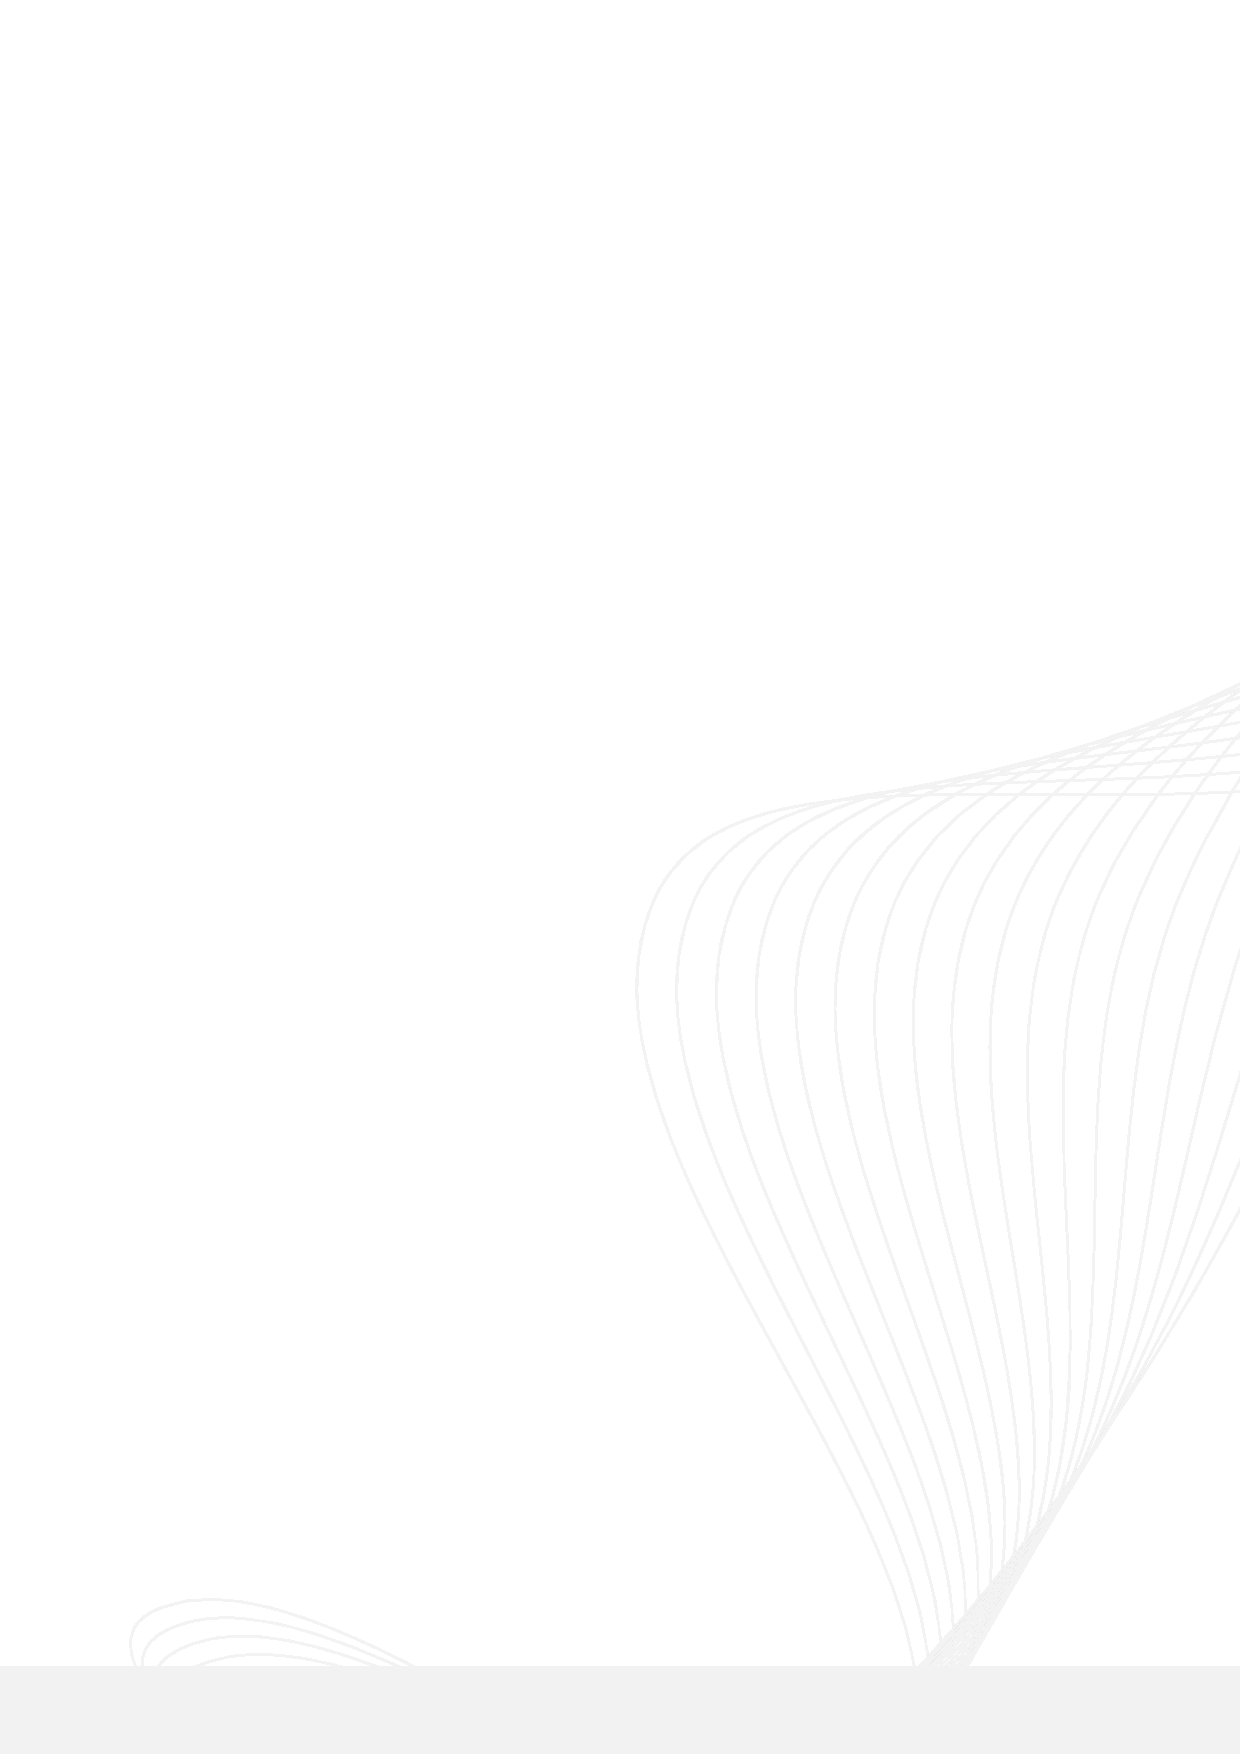
\includegraphics[width=\paperwidth,height=\paperheight]{Front-Page-BG.pdf}%
    }

\newpage

\pagestyle{plain}

\vspace*{0.2\textheight}

\noindent \enquote{\itshape "Le problème central de la prévention des dépressions économiques a été résolu, en pratique, pour de nombreuses décennies."}\bigbreak

\hfill Robert Lucas (prix Nobel d'économie 1995), \textit{Discours présidentiel à l'American Economic Association}, 2003.

\newpage

% Inclusion des sections
{\centering
\vspace*{\fill}
\section*{Remerciements}}
\addcontentsline{toc}{section}{Remerciements}
\begin{sloppypar}
  Nous tenons tout particulièrement à exprimer notre profonde gratitude à madame Françoise SEYTE pour sa bienveillance, son soutien indéfectible et le temps précieux qu'elle a généreusement consacré à l'encadrement de ce Projet d'Économétrie Financière. Son expertise, son dévouement et ses conseils éclairés ont été d'une importance capitale tout au long de cette étude, contribuant de manière significative à son aboutissement. Nous tenons également à exprimer ma reconnaissance à monsieur Roman MESTRE pour ses conseils avisés en macroéconomie monétaire. Ses connaissances approfondies et sa disponibilité ont été des atouts dans la compréhension des concepts complexes liés à cette étude. Ses précieuses remarques et ses éclairages ont enrichi ma réflexion et ont grandement contribué à la qualité de ce travail.  
\end{sloppypar}
\vspace*{\fill}

\newpage
{\centering
\vspace*{\fill}
\section*{Résumé}}
\addcontentsline{toc}{section}{Résumé}
\begin{sloppypar}
  Ce projet vise à modéliser les dynamiques des sous-indicateurs de stress systémique des marchés interbancaire, des changes et des actions à l’aide de données mensuelles de 2005 à 2023. Ces marchés, interdépendants et soumis à des tensions systémiques, sont étudiés à travers des approches économétriques non linéaires, notamment les modèles Markov Switching VAR et NARDL. Ces outils permettent de capturer les transitions entre régimes et les asymétries dans les réponses aux chocs financiers. En s’appuyant sur le Composite Indicator of Systemic Stress, le projet analyse les interconnexions entre ces marchés pour identifier les mécanismes de contagion et les périodes de forte instabilité. L’objectif est d’approfondir la compréhension des tensions systémiques et de fournir des outils pour anticiper les crises financières, renforcer la stabilité des marchés et guider les politiques économiques et macroprudentielles. 
\end{sloppypar}
\vspace*{\fill}

\newpage

% Sommaire réduit (limité aux sections seulement)
\shorttoc{Sommaire}{1}\addcontentsline{toc}{section}{Sommaire}

\newpage

% Sections principales
\section*{Introduction}\addcontentsline{toc}{section}{Introduction}

\begin{sloppypar}

La stabilité du système financier européen repose sur l’équilibre entre les différents segments de marché. Cependant, cet équilibre est régulièrement menacé par des tensions systémiques, amplifiées par l’interconnexion croissante des marchés et les mécanismes de contagion. Ces tensions, lorsqu’elles ne sont pas correctement identifiées, peuvent rapidement se propager et engendrer des crises financières globales, comme les crises des subprimes de 2008, la crise de la dette souveraine en Europe entre 2010 et 2012, et plus récemment la pandémie de COVID-19. Ces événements mettent en lumière la nécessité de disposer d’outils avancés pour comprendre et anticiper les dynamiques complexes qui sous-tendent les stress systémiques.\\

Dans ce contexte, le Composite Indicator of Systemic Stress (CISS) émerge comme un outil essentiel pour capter les signaux de stress financier. Ce dernier repose sur l’agrégation de cinq sous-indicateurs de stress spécifiques à trois segments financiers majeurs : le marché interbancaire, le marché des changes, le marché des actions, le marché actions et les intermédiaires financiers. Ces sous-indicateurs permettent de mesurer non seulement les tensions au sein de chaque marché, mais aussi les interactions dynamiques entre ces segments, particulièrement critiques en période de crise. Pourtant, la complexité des dynamiques de marché, exacerbée par de fortes volatilités avec des changements de régime et des effets asymétriques, rend leur modélisation particulièrement ardue.\\

En ce qui concerne la modélisation du stress systémique, des outils comme le CISS ont été développés pour fournir des mesures agrégées du stress financier. \cite[2012]{Hollo} ont conceptualisé le CISS, démontrant son utilité pour capturer les interconnexions et les corrélations dynamiques entre plusieurs segments financiers. D’autres travaux, tels que ceux de \cite[2013]{Duca et Peltonen}, ont souligné l’importance de cet indicateur pour la surveillance macroprudentielle, notamment en période de crise. Les recherches sur les mécanismes de contagion, comme les effets de liquidité et les ajustements de portefeuilles  \cite[2009]{Brunnermeier et Pedersen}, ont enrichi la compréhension des dynamiques de propagation des tensions. Ces contributions montrent que l’intégration des approches économétriques avancées dans l’analyse des stress systémiques est essentielle pour saisir les interactions complexes entre les marchés et orienter les politiques de stabilisation financière.\\

\textbf{Ainsi, les méthodes économétriques non linéaires peuvent-elles être utilisées pour modéliser et interpréter les interactions dynamiques entre les sous-indicateurs de stress systémique entre le marché actions, des changes et interbancaire, tout en intégrant les effets de régimes et les asymétries qui caractérisent les relations de stress entre ces sous-indicateurs ? Sur données mensuelles de 2005 à 2023.}\\

Cette problématique s’inscrit dans un cadre méthodologique avancé, visant à dépasser les limites des approches économétriques linéaires traditionnelles. En effet, les dynamiques systémiques des marchés financiers présentent des comportements complexes, notamment des transitions abruptes entre régimes (par exemple, entre périodes de faible et de forte volatilité) et des asymétries dans les réponses aux chocs financiers. Ces caractéristiques rendent les modèles non linéaires particulièrement adaptés pour capturer les structures sous-jacentes des interactions de stress sur les segments financiers. Ce projet vise donc à explorer ces dynamiques à travers la modélisation non-linéaire multivariée et univariée des sous-indicateurs de stress systémique pour la période 2005-2023 (données mensuelles). Deux approches économétriques complémentaires sont mises en œuvre pour répondre à la question posée.\\

Face à ces défis, la littérature en économétrie et en modélisation du stress systémique a apporté des premières solutions méthodologiques. D'une part, les modèles Markov Switching VAR (MS-VAR) proposés initialement par \cite[1989]{Hamilton}, ces modèles permettent de capturer les transitions entre régimes, en identifiant des états latents caractérisant les périodes de faible et de forte volatilité. Ils se révèlent particulièrement efficaces pour analyser les séries temporelles présentant des ruptures structurelles ou des comportements non stationnaires. Par exemple, \cite[2012]{Ang et Timmermann} ont montré leur pertinence dans l’étude des dynamiques financières cycliques. Dans le cadre de ce projet, ces modèles sont utilisés pour analyser les interactions dynamiques entre les sous-indicateurs, tout en tenant compte des changements structurels au fil du temps. D'autre part, les modèles NARDL (Non-linear Autoregressive Distributed Lag) : Introduits par \cite[2014]{Shin}, ces modèles se concentrent sur les dynamiques univariées, en intégrant des asymétries dans les réponses aux chocs. Ils permettent de distinguer les effets des variations positives et négatives sur une variable cible, une approche particulièrement pertinente pour les sous-indicateurs de stress financier, où les réponses aux tensions ne sont pas toujours symétriques. Leur application à la macroéconomie monétaire a été mise en avant par \cite[2013]{Balcilar et Ozdemir}, qui ont montré leur utilité pour modéliser les comportements asymétriques des marchés.\\

L’intégration de ces deux cadres méthodologiques permet de mieux capter la manière dont les tensions systémiques émergent, évoluent et se propagent au sein du système financier. Une attention particulière est portée à l’identification des mécanismes de contagion. Ces mécanismes sont modélisés en tenant compte des effets de régime et des asymétries observées dans les données.\\

Le projet ambitionne également d’éclairer la manière dont les autorités monétaires et macroprudentielles peuvent utiliser ces outils pour surveiller et stabiliser le système financier. En offrant des indicateurs précis et dynamiques, il devient possible de détecter les signaux précoces de crises systémiques et d’adopter des mesures préventives adaptées. Par exemple, une augmentation simultanée des tensions sur les marchés interbancaire, des changes et des actions pourrait indiquer un risque accru de propagation des tensions à l’ensemble du système financier.\\

L’analyse se concentre sur les données mensuelles couvrant la période 2005-2023, une période marquée par des crises financières majeures. Après une présentation des sous-indicateurs et des segments financiers étudiés, la méthodologie adoptée est détaillée, en insistant sur les spécificités des modèles MS-VAR et NARDL. Les résultats obtenus permettront d’identifier les périodes de stress systémique, d’évaluer l’intensité des interconnexions entre marchés, et de proposer des recommandations pour renforcer la résilience du système financier  pour le régulateur.\\

Ce projet s’inscrit dans une démarche visant à enrichir la compréhension des dynamiques non linéaires des marchés financiers. En combinant des approches économétriques avancées et des données empiriques riches, il est attendu que ces travaux contribuent significativement à l’étude des stress systémiques, tout en offrant des outils robustes pour guider les politiques monétaires et macroprudentielles.

\end{sloppypar}
\newpage
\section{L'indicateur composite de stress systémique}

\begin{sloppypar}

La stabilité du système financier repose sur l'équilibre des interactions entre les différents segments de marché. Cependant, cet équilibre est régulièrement menacé par des tensions systémiques, amplifiées par l'interconnexion croissante des marchés. Dans ce contexte, des outils d'analyse et de surveillance, tels que le \textit{Composite Indicator of Systemic Stress} (\textit{CISS}), se révèlent essentiels pour comprendre et anticiper les risques systémiques. Conçu pour capturer les signaux de stress financier à travers différents segments, cet indicateur composite intègre les spécificités des marchés actions, des changes, obligataire, des intermédiaires financiers et monétaires, tout en tenant compte de leurs interactions dynamiques.\\

Le premier sous-paragraphe introduit les fondements du \textit{CISS}, en expliquant son objectif principal : fournir une mesure agrégée du stress systémique tout en capturant les interdépendances entre les segments de marché. Elle explore également son évolution depuis des outils plus sectoriels, tels que le \textit{SovCISS}, jusqu'à sa formulation actuelle, qui intègre des notions de corrélation dynamique entre marchés. Une attention particulière est portée à la formulation mathématique du \textit{CISS}, mettant en évidence les méthodologies de pondération et de calcul des sous-indicateurs.\\

Le second sous-paragraphe se concentre sur les variables sélectionnées du \textit{CISS} pour ce projet. Ces variables reflètent les dynamiques de trois segments financiers majeurs : le marché des changes (FOREX), le marché des actions (Equity) et le marché monétaire (IMM). Pour chaque segment, les spécificités du fonctionnement, les déterminants des tensions et les implications systémiques des variations sont discutés. Cette analyse permet de mieux comprendre comment chaque sous-indicateur reflète le stress sur son segment respectif et contribue à la mesure globale du risque systémique pour la BCE.\\

Enfin, le troisième sous-paragraphe analyse l'interconnexion et la contagion entre les sous-indicateurs, en insistant sur les mécanismes qui amplifient les tensions au sein du système financier. Les interactions entre les marchés des actions, des changes et monétaires sont examinées pour montrer comment les tensions dans un segment peuvent se propager à d'autres segments, créant un effet domino. Les mécanismes de contagion, tels que la propagation via la liquidité ou la fuite vers la qualité, ainsi que le rôle des politiques monétaires et macroprudentielles, sont discutés en détail.

\subsection{Construction de l'indicateur composite de stress systémique}

Le \textit{CISS} est un outil central pour surveiller les tensions systémiques, en offrant une mesure agrégée du stress financier à travers différents segments de marché. Cette sous-section explore d’abord sa présentation générale, en détaillant son rôle dans l’identification des risques systémiques. Ensuite, l’évolution de cet indicateur depuis le \textit{SovCISS} est discutée, mettant en lumière son passage d’un indicateur centré sur les obligations souveraines à une approche globale intégrant plusieurs segments financiers. Enfin, sa formulation mathématique est présentée, expliquant comment les sous-indicateurs sont normalisés, pondérés et agrégés pour refléter les interconnexions et les corrélations dynamiques entre les marchés. Cette structure vise à clarifier la construction et l’utilité de cet outil dans la gestion des risques financiers.

\subsubsection{Généralités}

Le \textit{CISS} est un outil clé pour la surveillance de la stabilité financière dans les économies modernes, notamment au sein de l'Union européenne. Conçu pour offrir une vue d'ensemble des tensions sur les marchés financiers, cet indicateur composite permet aux régulateurs, en particulier la Banque Centrale Européenne (BCE), d’évaluer le risque systémique en temps réel et d’adapter leurs politiques en conséquence. Le \textit{CISS} a pour objectif principal de détecter les périodes où les tensions financières se manifestent simultanément sur plusieurs segments des marchés, ce qui reflète un risque accru de perturbation de l’ensemble du système financier.\\

Le stress systémique désigne la situation où une instabilité financière locale ou sectorielle s'étend et affecte la stabilité de l'ensemble du système financier. Cette extension peut être provoquée par des interconnexions entre différents segments des marchés financiers, des comportements synchronisés des acteurs économiques, ou encore par des canaux de contagion tels que la liquidité ou la confiance des investisseurs. Lorsqu'une crise se généralise, elle peut perturber le fonctionnement normal des marchés, compromettant ainsi la fourniture de crédit, la stabilité des taux d'intérêt et des taux de change, ainsi que le bon déroulement des institutions financières. Cela peut, à terme, affecter gravement l'économie réelle en réduisant la croissance, en augmentant le chômage et en déstabilisant les secteurs productifs.\\

Dans ce contexte, le \textit{CISS} permet de capter les signaux de tensions financières à travers différents marchés, qu'il s'agisse du marché des actions, des obligations, du marché monétaire ou des changes. En captant ces signaux simultanément, le \textit{CISS} évalue si les tensions dans un segment particulier sont susceptibles de se propager aux autres segments, créant un effet de contagion susceptible de perturber l’ensemble du système financier.\\

Le \textit{CISS} se base sur l'idée que les marchés financiers ne fonctionnent pas en autarcie. Au contraire, ils sont fortement interconnectés, et une crise dans l'un d'eux peut rapidement se propager aux autres via divers canaux. Par exemple, une crise de liquidité sur le marché monétaire peut forcer les banques à vendre massivement leurs actifs financiers, y compris des actions ou des obligations, pour couvrir leurs besoins en liquidité, ce qui augmente la volatilité sur les marchés des actions et obligataires. De même, des fluctuations importantes sur le marché des changes, par exemple une dépréciation rapide d'une monnaie majeure comme l'euro ou le dollar, peuvent provoquer des ajustements significatifs dans les portefeuilles des investisseurs et des entreprises, avec des répercussions sur les marchés actions et obligations. \\

Ce dernier tient compte de ces interconnexions en agrégeant plusieurs sous-indicateurs de stress issus de différents segments du marché. Ces sous-indicateurs mesurent des aspects spécifiques du stress financier, comme la volatilité des prix des actions, les écarts de taux entre les obligations souveraines et les obligations d'entreprises, ou encore les tensions sur les taux interbancaires. En combinant ces informations dans un seul indicateur composite, le CISS offre une mesure globale du risque systémique, tout en accordant une attention particulière aux périodes où les tensions apparaissent simultanément sur plusieurs segments des marchés.\\

Aussi, des caractéristiques majeures de l'indicateur sont qu'il accorde une importance particulière aux corrélations dynamiques entre les différents segments du marché. En période normale, les tensions sur un marché peuvent rester localisées et ne pas se propager aux autres segments. Cependant, en période de crise, ces corrélations tendent à augmenter, ce qui signifie que les chocs dans un segment particulier, comme le marché des actions, ont plus de chances de se transmettre aux autres segments, comme le marché des changes ou le marché monétaire. Le CISS capture cette augmentation des corrélations en attribuant un poids plus important aux périodes où plusieurs marchés sont simultanément sous pression. Ainsi, plus les tensions sont corrélées entre les marchés, plus le CISS augmentera, signalant un risque systémique accru. Cette approche permet de différencier les périodes de stress localisé, qui peuvent ne pas représenter un risque pour l'ensemble du système financier, des périodes de stress systémique, où la contagion entre les segments du marché est plus probable. Cela aide les régulateurs à concentrer leurs efforts sur les périodes où les risques systémiques sont les plus élevés et à ajuster leur politique monétaire ou macroprudentielle en conséquence.\\

L'une des raisons pour lesquelles le CISS est particulièrement précieux pour les régulateurs comme la BCE est qu'il permet de détecter les risques avant qu'ils ne deviennent visibles à travers d'autres indicateurs économiques. En surveillant en permanence l'état des différents segments des marchés financiers, le CISS permet aux régulateurs de réagir de manière proactive aux signes de stress systémique. Cela est particulièrement important dans les économies modernes, où les marchés financiers jouent un rôle essentiel dans l'allocation des ressources et le financement de l'activité économique. De plus, le CISS est un outil précieux pour la politique macroprudentielle, qui vise à prévenir les crises financières avant qu'elles ne se matérialisent. En identifiant les périodes de risque systémique élevé, les régulateurs peuvent prendre des mesures pour renforcer la résilience du système financier, pour illustrer en augmentant les exigences de fonds propres des banques, en imposant des limites sur l'exposition aux risques ou en renforçant les liquidités des institutions financières. L'objectif est de prévenir la contagion des crises financières, de sorte que même en cas de choc sur un segment particulier du marché, le reste du système financier reste suffisamment solide pour absorber ce choc sans s'effondrer.\\

Ainsi, l'utilité de l'indicateur ne se limite pas à la surveillance des marchés financiers. Il joue également un rôle crucial dans la protection de l'économie réelle contre les perturbations financières. Lorsqu'une crise financière devient systémique, elle affecte non seulement les marchés financiers, mais aussi l'économie dans son ensemble. Les entreprises trouvent plus difficile de se financer, les ménages réduisent leurs dépenses en raison des incertitudes économiques, et les banques deviennent plus réticentes à prêter, ce qui aggrave encore la contraction de l'activité économique. En aidant à prévenir les crises systémiques, le CISS contribue indirectement à la stabilité de l'économie réelle, en assurant que les marchés financiers continuent de fonctionner de manière fluide, même en période de tension.\\ 

Après ces généralités il convient de comprendre l'histoire de l'indicateur avant d'aborder son développement.

\subsubsection{Du SovCISS au CISS}

Avant l'introduction du \textit{CISS}, la Banque Centrale Européenne (BCE) et d'autres institutions financières utilisaient un autre indicateur appelé \textit{SovCISS} (Sovereign Composite Indicator of Systemic Stress), conçu spécifiquement pour mesurer le stress systémique lié aux marchés des obligations souveraines. Le \textit{SovCISS} a été développé à une époque où les crises de dette souveraine, en particulier celles qui ont frappé la zone euro entre 2010 et 2012, étaient au centre des préoccupations des régulateurs. Cet indice visait à capter les tensions sur les marchés des obligations d'État, en tenant compte des spreads entre les obligations souveraines des pays membres de la zone euro et les obligations dites « sans risque », comme celles de l'Allemagne. En période de crise, les écarts entre les taux d’intérêt des obligations d’États comme ceux de la Grèce ou de l’Italie par rapport à l’Allemagne augmentaient de manière significative, signalant une perte de confiance des investisseurs dans la capacité des gouvernements à honorer leurs dettes.\\

Cependant, bien que le \textit{SovCISS} ait été un outil utile pour comprendre les dynamiques de la crise de la dette souveraine, il est devenu évident qu'un indice uniquement centré sur les obligations souveraines était insuffisant pour mesurer les risques systémiques globaux. Les crises financières récentes, comme celle des subprimes de 2007-2008, ont montré que les crises systémiques ne se limitaient pas à un seul segment, mais résultaient d'une propagation rapide des tensions entre les différents marchés financiers. Ainsi, la BCE a reconnu la nécessité de développer un indicateur plus global, capable de capter les interactions et les tensions simultanées à travers plusieurs segments financiers, tels que les marchés des changes, des actions, des obligations privées, et des banques. C’est dans ce contexte que le \textit{CISS} a été introduit.\\

Le \textit{CISS} surpasse le \textit{SovCISS} en ce qu’il intègre une mesure de la corrélation dynamique entre les segments du marché. Alors que le \textit{SovCISS} se concentrait principalement sur les tensions dans le secteur des obligations souveraines, le \textit{CISS} capte les tensions qui se propagent à travers tous les segments, offrant ainsi une vision plus complète du stress systémique. Il permet non seulement de surveiller les tensions dans chaque segment, mais aussi d’évaluer comment ces tensions interagissent et s’amplifient entre eux. Le passage du \textit{SovCISS} au \textit{CISS} est une évolution dans la manière dont les régulateurs financiers, et en particulier la BCE, appréhendent les crises systémiques : d’une approche sectorielle centrée sur les obligations souveraines à une approche globale qui prend en compte l'ensemble des segments du système financier et leurs interconnexions.

\subsubsection{Le développement du \textit{CISS}}

Les crises financières récentes, notamment la crise des subprimes de 2007-2008, ont montré à quel point les chocs financiers pouvaient rapidement se propager à travers différents segments du système financier, déclenchant ainsi des crises systémiques d’une ampleur sans précédent. Avant la création du \textit{CISS}, les outils de surveillance disponibles, bien qu'utiles pour comprendre certains aspects des marchés financiers, étaient trop fragmentés et ne permettaient pas de saisir pleinement l'ampleur ni la portée des risques systémiques. Ces outils étaient principalement axés sur des indicateurs spécifiques à chaque segment, tels que les taux interbancaires, les spreads obligataires ou la volatilité des marchés actions, sans intégrer de manière adéquate les interconnexions entre les différents segments. Cela créait une lacune dans la surveillance globale des risques financiers, notamment en ce qui concerne l’anticipation de crises systémiques.\\

L'indicateur répond à ce besoin en fournissant une mesure agrégée du stress systémique, capable de capturer les tensions qui surviennent simultanément dans plusieurs secteurs du système financier. Ce cadre analytique plus intégré s’est révélé essentiel après la crise des subprimes, une période où les indicateurs traditionnels avaient échoué à identifier les signes avant-coureurs d’une crise mondiale. La crise de 2007-2008 a particulièrement mis en lumière les insuffisances des indicateurs sectoriels pour surveiller et anticiper les risques financiers. Les outils utilisés à cette époque étaient trop compartimentés, focalisés sur des segments isolés des marchés, ce qui empêchait de saisir l'ampleur des interconnexions et de l’effet de contagion qui allait finalement provoquer un effondrement général du système financier. Le CISS a été conçu pour combler cette lacune en offrant une vue d’ensemble des risques systémiques en agrégeant les tensions dans les principaux segments financiers : le secteur bancaire, les marchés obligataires, les marchés des actions, les marchés des changes, et d’autres segments financiers clés.\\

Son développement repose sur des concepts tirés de la théorie des portefeuilles, développée par Harry Markowitz dans les années 1950. Cette théorie met en évidence le rôle crucial de la diversification pour optimiser un portefeuille d’actifs en termes de rentabilité maximale et de risque minimal. De la même manière, cet indicateur applique ce principe à la gestion du risque systémique en combinant plusieurs segments du système financier tout en tenant compte des corrélations temporelles entre eux. Chaque segment est susceptible de subir des chocs qui peuvent se propager aux autres segments par le biais de multiples canaux de transmission. L’indicateur reflète donc non seulement les tensions dans chaque segment, mais aussi la manière dont ces tensions interagissent et s’amplifient à travers les interconnexions systémiques. Cela en fait un outil global particulièrement pertinent pour mesurer le risque systémique à un instant donné.\\

En outre, cet indicateur permet de surveiller en temps réel les tensions qui se manifestent dans les différents segments du système financier. Cela en fait un outil particulièrement précieux pour les banques centrales et les autorités financières, car il leur offre la possibilité de détecter les signes précoces de crises potentielles et de mettre en place des mesures préventives pour stabiliser le système. En identifiant les périodes de stress simultané sur plusieurs segments, il permet d’anticiper les crises avant qu’elles ne deviennent trop graves et d’intervenir de manière proactive. Il constitue également un outil d’analyse rétrospective, permettant d’examiner les crises passées et d’évaluer les niveaux de stress atteints durant ces périodes critiques. Cela permet d’établir des comparaisons entre différentes crises financières et d’en analyser les dynamiques propres, facilitant ainsi l’évaluation des politiques et des mesures mises en place pour répondre à ces crises.\\

Par exemple, en comparant les niveaux atteints durant la crise des subprimes à ceux observés pendant la crise de la dette souveraine en Europe, il est possible d’évaluer l’efficacité des réponses monétaires et fiscales appliquées dans chacun de ces cas. Ce type d’analyse comparative permet également de tirer des enseignements utiles pour la gestion des futures crises. Une analyse approfondie des dynamiques de chaque crise aide les régulateurs à mieux comprendre les mécanismes de propagation des tensions financières et à ajuster leurs outils en conséquence.\\

Cet indicateur agit également comme un outil de rétroaction particulièrement utile pour les décideurs politiques et monétaires. Après une intervention de la banque centrale, une baisse significative de l’indicateur signalerait que les mesures prises ont effectivement contribué à réduire les tensions dans le système financier. Cette capacité d’évaluer les réponses politiques et monétaires en temps réel confère à cet outil un rôle unique dans la gestion des crises financières. Contrairement aux indicateurs traditionnels qui ne captent que des aspects isolés du marché, il permet une vision plus holistique des risques, facilitant ainsi des réponses politiques plus efficaces et mieux ciblées.\\

Il est décomposé en cinq indices principaux, chacun représentant un segment majeur du marché financier, tels que le secteur bancaire, les marchés obligataires, les marchés des actions, les marchés des changes et les autres segments financiers pertinents. Chacun de ces indices est ensuite subdivisé en sous-indices qui capturent des aspects spécifiques de leurs segments respectifs, comme la volatilité des actions, les spreads des obligations souveraines ou les tensions sur les taux interbancaires. Cette structure hiérarchisée permet à l’outil d’offrir une vision à la fois large et détaillée des tensions financières, tout en tenant compte des interdépendances entre les segments. L’agrégation de ces indices, en tenant compte des corrélations entre eux, permet de générer un indicateur composite qui mesure le niveau global de risque systémique auquel est confronté le système financier.\\

L’innovation apportée par cet indicateur réside donc dans sa capacité à offrir une mesure intégrée et dynamique des risques financiers. Contrairement aux approches traditionnelles, qui se concentrent sur l’intensité des tensions dans des segments spécifiques, il prend en compte la propagation et la diffusion de ces tensions à travers l’ensemble du système financier. Cela permet aux régulateurs de mieux comprendre la manière dont les chocs financiers se propagent entre les différents segments et d’anticiper l’apparition de crises systémiques. En intégrant à la fois l’intensité des tensions et leur diffusion à travers le système, cet outil devient central pour la gestion et l’anticipation des crises financières.


%Graphique 


\subsubsection{Formulation mathématique du \textit{CISS}}


Comme présenté dans le schéma, le \textit{CISS} repose sur cinq indices, chacun étant lui-même subdivisé en plusieurs sous-indices. Ces indices principaux sont pondérés en fonction de leur importance relative, avec des coefficients spécifiques attribués à chaque sous-indice, ce qui permet d'obtenir une mesure globale du risque systémique. Les poids attribués aux indices déterminent leur influence sur le calcul final du \textit{CISS}.

\begin{enumerate}
    \item  30\% pour le marché intermédiaire
    \item 25\% pour le marché des actions 
    \item 15\% pour le marché obligataire 
    \item 15\% pour le marché monétaire
    \item 15\% pour le marché des changes
\end{enumerate}

Premièrement, pour chaque segment de marché, trois indicateurs de stress financier sont sélectionnés, notés \( x_{t,i,j} \). Soit un ensemble de valeurs observées \( x_1, x_2, \dots, x_n \) pour un indicateur spécifique. On ordonne ces valeurs de telle sorte que \( x_{[1]} \leq x_{[2]} \leq \dots \leq x_{[n]} \), où \( x_{[r]} \) représente le \( r \)-ième ordre de valeur. De plus,


\begin{itemize}
    \item \( t \) représente le temps,
    \item \( i \) indique le segment de marché (\( i = 1, 2, 3, 4, 5 \) pour les marchés monétaires, obligations, actions, intermédiaires financiers, et changes),
    \item \( j \) correspond à chaque indicateur spécifique dans le segment (\( j = 1, 2, 3 \)).
\end{itemize}

Ces indicateurs sont normalisés en utilisant leur fonction de distribution cumulative empirique \( F(x_{t,i,j}) \), ce qui donne le score normalisé :
\[
z_{t,i,j} = F(x_{t,i,j}) = \frac{r}{n}
\]
où \( r \) est le rang de \( x_{t,i,j} \) dans un ensemble de \( n \) observations, ordonnées de manière croissante. La transformation est mise à jour de manière récursive pour chaque nouvelle observation \( T \) :
\[
z_{T,i,j} = F_{T}(x_{T,i,j}) = \frac{r}{T}
\]

Deuxièmement, pour chaque segment de marché \( i \), un sous-indice \( s_{t,i} \) est construit en prenant la moyenne arithmétique des trois indicateurs normalisés :
\[
s_{t,i} = \frac{1}{3} \sum_{j=1}^{3} z_{t,i,j}
\]

Enfin, les cinq sous-indices sont agrégés dans un indicateur composite \( CISS_t \) en utilisant des poids \( w_i \) représentant leur importance pour l'activité économique réelle. Le vecteur de poids est \( w = [0.15, 0.15, 0.25, 0.30, 0.15] \). Le CISS est calculé en tenant compte des corrélations dynamiques entre les segments :
\[
CISS_t = \left( w \circ s_t \right)^T C_t \left( w \circ s_t \right) = \sum_{i=1}^{5} \sum_{j=1}^{5} w_i w_j s_{t,i} s_{t,j} \rho_{t,ij}
\]
où \( w \circ s_t \) représente le produit de Hadamard (élément par élément) entre le vecteur de poids \( w \) et le vecteur des sous-indices \( s_t = [s_{t,1}, s_{t,2}, s_{t,3}, s_{t,4}, s_{t,5}] \), et \( C_t \) est la matrice de corrélation des sous-indices.\\

Aussi, la matrice de corrélation \( C_t \) est une matrice symétrique \( 5 \times 5 \), où chaque élément \( \rho_{t,ij} \) représente la corrélation entre les sous-indices \( s_{t,i} \) et \( s_{t,j} \) :

\begin{equation}
C_t = \begin{bmatrix}
1 & \rho_{t,12} & \rho_{t,13} & \rho_{t,14} & \rho_{t,15} \\
\rho_{t,12} & 1 & \rho_{t,23} & \rho_{t,24} & \rho_{t,25} \\
\rho_{t,13} & \rho_{t,23} & 1 & \rho_{t,34} & \rho_{t,35} \\
\rho_{t,14} & \rho_{t,24} & \rho_{t,34} & 1 & \rho_{t,45} \\
\rho_{t,15} & \rho_{t,25} & \rho_{t,35} & \rho_{t,45} & 1 \\
\end{bmatrix}
\end{equation}


Les éléments de la matrice \( C_t \) sont calculés en fonction des covariances \( \sigma_{t,ij} \) et des écarts-types des sous-indices respectifs \( \sigma_{t,i} \) et \( \sigma_{t,j} \) :
\[
\rho_{t,ij} = \frac{\sigma_{t,ij}}{\sqrt{\sigma_{t,i}^2 \cdot \sigma_{t,j}^2}}
\]
Les covariances et variances sont calculées de manière récursive avec des moyennes mobiles exponentielles :
\[
\sigma_{t,i}^2 = \lambda \sigma_{t-1,i}^2 + (1 - \lambda) \tilde{s}_{t,i}^2
\]
\[
\sigma_{t,ij} = \lambda \sigma_{t-1,ij} + (1 - \lambda) \tilde{s}_{t,i} \tilde{s}_{t,j}
\]
où \( \lambda \) est un paramètre de lissage, typiquement autour de 0.93, et \( \tilde{s}_{t,i} \) est le sous-indice centré autour de sa moyenne historique.\\










Dans le cadre de cette étude, trois segments clés du système financier seront examinés en détail : le marché des changes, le marché des actions, et le marché interbancaire. L'analyse de ces segments permettra d'obtenir une vue d'ensemble des dynamiques spécifiques à chacun de ces marchés.\\

Après que les sous-indicateurs propres à chaque segment du marché financier ont été analysés, il est essentiel que l’interconnexion entre ces segments soit examinée. En effet, il est observé que les tensions sur un marché ne restent pas isolées, mais peuvent être propagées et affecter d'autres segments. L'importance des mécanismes de contagion sera ainsi mise en lumière, en montrant leur rôle central dans l'amplification du stress systémique. Ces interactions et leurs implications pour la stabilité financière globale seront désormais étudiées.

\subsection{Cadre conceptuel des sous-indicateurs étudiés}

Dans le cadre de ce projet des sous-indicateurs de stress systémique, trois segments sont sélectionnés : le marché des changes, le marché des actions et le marché monétaire. Ces marchés, tous interconnectés, jouent un rôle crucial dans la stabilité financière globale. Chacun de ces segments réagit aux chocs économiques, monétaires et politiques, influençant ainsi l'ensemble du système financier. Leur analyse permet de mieux comprendre la propagation des risques et d'anticiper des périodes de stress systémique.

\subsubsection{Marché des changes (FOREX)}

Le marché des changes, communément appelé FOREX (Foreign Exchange Market), est le plus vaste et le plus liquide au monde. Il est au cœur des transactions financières internationales, car il permet l'échange de devises entre différents acteurs économiques. Fonctionnant 24 heures sur 24, cinq jours par semaine, ce marché est non seulement crucial pour le commerce international, mais aussi pour les investissements transfrontaliers et la gestion des risques de change.\\

Sur le FOREX, les devises sont échangées par paires, ce qui signifie qu'une devise est toujours cotée par rapport à une autre. Les variations des taux de change reflètent donc la valeur relative d'une devise par rapport à une autre. Ces variations peuvent être influencées par une multitude de facteurs économiques, notamment les taux d'intérêt, l'inflation, la balance commerciale et les décisions des banques centrales, mais aussi par des événements politiques ou des crises géopolitiques. La liquidité exceptionnelle de ce marché est due à sa structure décentralisée : les transactions sont réalisées à travers des réseaux interbancaires et ne passent pas par une plateforme centralisée, ce qui offre une flexibilité accrue mais pose également des défis en termes de surveillance et de régulation.\\

L’un des rôles essentiels du marché des changes est de permettre aux entreprises de couvrir leurs risques de change, en particulier lorsque leurs opérations s’étendent au-delà des frontières nationales. Une fluctuation des taux de change peut avoir un impact significatif sur les résultats financiers d’une entreprise, car elle modifie la valeur des flux de trésorerie en devises étrangères. Le FOREX permet également aux investisseurs de diversifier leurs portefeuilles en achetant et vendant des devises pour tirer parti des variations de taux.\\

Les banques centrales, comme la Banque Centrale Européenne (BCE), surveillent étroitement les mouvements sur le FOREX, car les variations trop importantes des taux de change peuvent déstabiliser les économies nationales. En cas de volatilité excessive, elles peuvent intervenir sur le marché pour stabiliser leur monnaie, en ajustant les taux d’intérêt ou en utilisant leurs réserves de devises. Le FOREX est divisé en deux types principaux de transactions : les opérations au comptant et les opérations à terme. Les opérations au comptant, ou "spot", consistent à acheter une devise contre une autre au taux de change actuel, avec une livraison généralement effectuée dans les deux jours suivant la transaction. Les opérations à terme, quant à elles, consistent à fixer à l'avance un prix, une quantité et une date pour un échange futur, offrant ainsi une couverture contre les fluctuations des taux de change. Ce marché à terme (ou "forward") est particulièrement important pour les entreprises multinationales qui cherchent à se protéger contre la volatilité future des devises.\\

Le sous-indicateur de stress du marché des changes mesure la volatilité des principales paires de devises, notamment l'euro contre le dollar américain, la livre sterling, ou le yen japonais. Une forte volatilité sur ce marché est souvent un signal précurseur de tensions économiques, politiques ou financières. En effet, lorsque les taux de change varient fortement, cela reflète souvent des ajustements majeurs dans les portefeuilles des investisseurs, des déséquilibres dans les flux de capitaux ou des événements politiques soudains qui affectent la stabilité des devises.\\

Pour la BCE et les régulateurs européens, cet indicateur permet de surveiller les risques systémiques pouvant découler d'une volatilité accrue du FOREX. Une volatilité excessive peut, par exemple, entraîner des mouvements importants de capitaux transfrontaliers, affectant ainsi la stabilité des marchés financiers européens. Par ailleurs, des variations brusques des taux de change peuvent également avoir un impact sur la compétitivité des entreprises européennes, notamment les exportateurs, en modifiant la valeur de leurs revenus en devises étrangères.

\subsubsection{Marché des actions (Equity)}

Le marché des actions est l'endroit où les actions des entreprises sont achetées et vendues. Ces actions représentent des parts de propriété dans les entreprises, et confèrent à leurs détenteurs des droits, tels que le droit de vote lors des assemblées générales ou encore le droit de recevoir des dividendes lorsque l'entreprise réalise des bénéfices. Le marché des actions est crucial à la fois pour les entreprises et pour les investisseurs, car il permet aux entreprises de lever des capitaux pour financer leur expansion, tandis qu’il offre aux investisseurs la possibilité d'obtenir un rendement sur leur capital.\\

L’introduction en bourse, ou IPO (Initial Public Offering), est l’un des mécanismes par lequel une entreprise lève des fonds sur le marché primaire en émettant des actions pour la première fois. Les investisseurs achètent ces actions directement auprès de l'entreprise émettrice. Une fois que les actions sont émises, elles peuvent être librement échangées sur le marché secondaire, où les prix fluctuent en fonction de l'offre et de la demande. C'est ce marché secondaire, souvent représenté par des places boursières comme Euronext ou la Bourse de Francfort, qui détermine la valorisation des entreprises et la performance des indices boursiers.\\

Le marché des actions est influencé par une variété de facteurs, notamment les résultats financiers des entreprises, les perspectives économiques, les taux d'intérêt, et les événements géopolitiques. Par nature, ce marché est volatil, car il réagit rapidement aux nouvelles économiques et politiques. La volatilité des marchés actions peut avoir des répercussions importantes sur la richesse des ménages et la capacité des entreprises à financer leurs projets. Une chute brutale des prix des actions peut entraîner une réduction de la consommation et des investissements, augmentant ainsi les risques pour l'économie réelle.\\

Le sous-indicateur de stress du marché des actions permet d’évaluer la volatilité des indices boursiers, les pertes cumulées au fil du temps, et les corrélations entre les actions et les obligations. Une hausse de cet indicateur signale souvent une perte de confiance des investisseurs dans les perspectives économiques et financières. Les investisseurs réagissent en vendant des actifs risqués, comme les actions, pour se réfugier dans des actifs plus sûrs, comme les obligations d'État, phénomène connu sous le nom de "fuite vers la qualité" (flight-to-quality).\\ 

Le sous-indicateur de stress du marché des actions revêt une importance particulière dans l'évaluation des risques systémiques. Une volatilité excessive sur ce marché peut non seulement entraîner des pertes significatives pour les investisseurs, mais aussi affecter l'économie réelle en rendant plus difficile l'accès au financement pour les entreprises. De plus, les fluctuations du marché des actions peuvent avoir un effet de contagion sur les autres marchés, en particulier le marché des changes, où une fuite massive de capitaux peut affecter la stabilité des devises.

\subsubsection{Marché monétaire (IMM)}

Le marché monétaire, ou marché interbancaire, est un marché réservé aux banques et institutions financières qui échangent entre elles des liquidités à très court terme. Ce marché joue un rôle central dans le bon fonctionnement du système bancaire, car il permet aux banques de gérer leur liquidité quotidienne, en empruntant ou en prêtant des fonds pour des durées allant de quelques jours à un an. Le marché monétaire est également essentiel pour la mise en œuvre de la politique monétaire des banques centrales, car il détermine les taux d'intérêt à court terme qui influencent l'ensemble du système financier.\\

Les transactions sur le marché monétaire se font généralement sur la base du taux d’intérêt interbancaire, tel que l’EONIA (Euro Overnight Index Average) ou l’Euribor (Euro Interbank Offered Rate). Ces taux d'intérêt servent de référence pour de nombreux autres taux dans l'économie, y compris les taux des prêts aux entreprises et aux ménages. Par conséquent, toute tension sur le marché monétaire peut rapidement se propager à l'ensemble de l'économie, en augmentant le coût du crédit et en réduisant la disponibilité des financements.\\

Le marché interbancaire fonctionne de manière décentralisée, les banques négociant directement entre elles sans passer par une plateforme centralisée. Cela permet une plus grande flexibilité, mais peut également accroître les risques en période de stress, lorsque la confiance entre les banques se détériore. Les crises de liquidité, comme celle de 2008, sont des exemples frappants de la manière dont les tensions sur le marché interbancaire peuvent provoquer un gel des liquidités et une crise financière généralisée.\\

Le sous-indicateur de stress du marché monétaire mesure les variations des taux interbancaires, ainsi que les écarts entre ces taux et ceux des obligations d'État. Une hausse rapide de ces écarts est souvent le signe de tensions sous-jacentes dans le système bancaire. Par exemple, lorsque les banques deviennent réticentes à se prêter mutuellement des fonds, cela reflète une méfiance accrue quant à la solvabilité des contreparties. En période de stress, les taux interbancaires peuvent augmenter de manière significative, rendant plus difficile et coûteux pour les banques de financer leurs activités.\\

Ce sous-indicateur est particulièrement important pour surveiller la santé du système bancaire et la stabilité financière globale. Une hausse des taux sur le marché monétaire peut rapidement entraîner une crise de liquidité, où les banques sont forcées de vendre des actifs ou de restreindre leurs prêts, amplifiant ainsi les tensions sur les autres segments financiers.\\

Après avoir analysé le cadre conceptuel théorique des trois marchés sectionnés. Il convient ensuite d'analyser les sous-indicateurs de ces marchés sur la période étudiée.

\subsubsection{Analyse des indicateurs entre janvier 2005 et décembre 2004}

L'évolution des sous-indicateurs de stress des trois principaux segments financiers : le marché monétaire, le marché des actions et le marché des changes est analysé sous un angle graphique dans la \autoref{fig:graphindicateurs} puis par rapport aux statistiques descriptives dans le \autoref{fig:statsdescriptives}.

\begin{figure}[H]
    \centering
    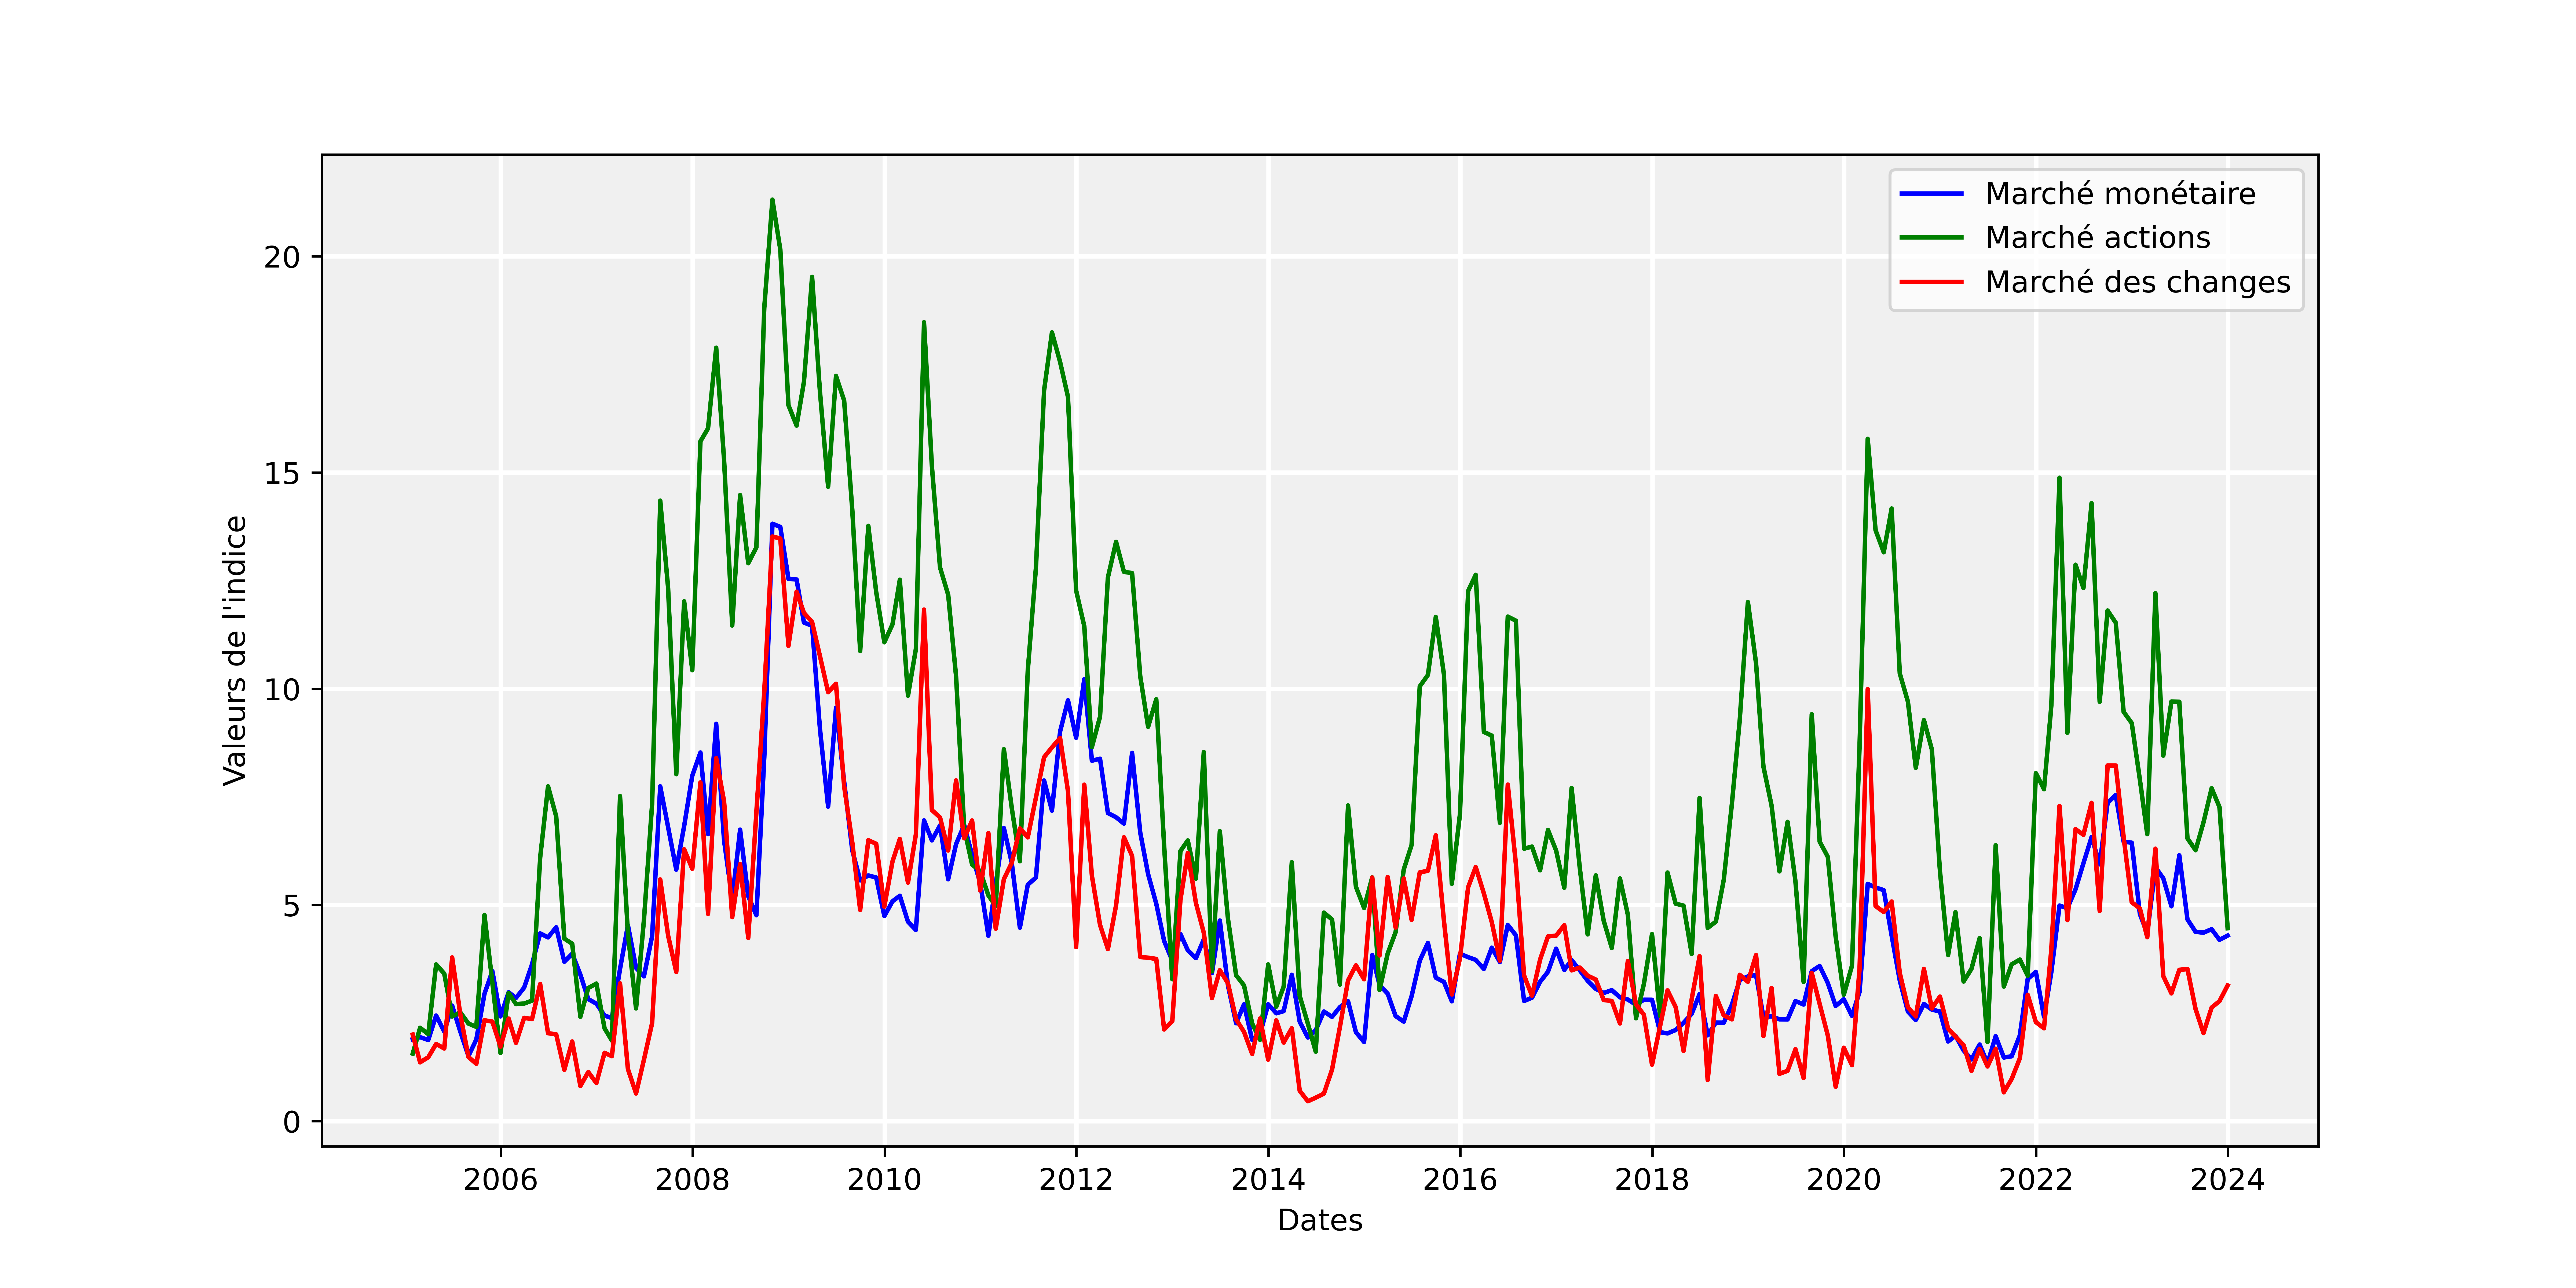
\includegraphics[width=1\linewidth]{figures/sous_indicateurs_stress.png}
    \caption{Sous-indicateurs de stress entre janvier 2005 et décembre 2024.}
    \label{fig:graphindicateurs}
\end{figure}

Le graphique montre l'évolution des sous-indicateurs de stress des trois principaux segments financiers (marché monétaire, marché des actions, et marché des changes) entre janvier 2005 et décembre 2024. Chaque indicateur est représenté par une courbe distincte : le marché monétaire est en bleu, le marché des actions en vert, et le marché des changes en rouge.\\

Le marché des actions montre la plus grande volatilité parmi les trois indicateurs. À plusieurs reprises, notamment entre 2008 et 2012 ainsi que vers 2020, on observe des pics marqués, correspondant à des périodes de forte tension sur ce marché. Le stress sur le marché des actions est particulièrement élevé lors des crises financières, comme celle de 2008, où le graphique montre une nette augmentation du stress. Après cette période de crise, le stress sur le marché des actions diminue progressivement, bien que des pics sporadiques apparaissent, notamment en 2020, ce qui pourrait être attribué à la crise liée à la pandémie de COVID-19. En général, la courbe verte représente des variations assez brusques, ce qui reflète la nature plus volatile du marché des actions, particulièrement sensible aux événements macroéconomiques et aux changements dans les conditions du marché mondial.

\begin{figure}[H]
    \centering
    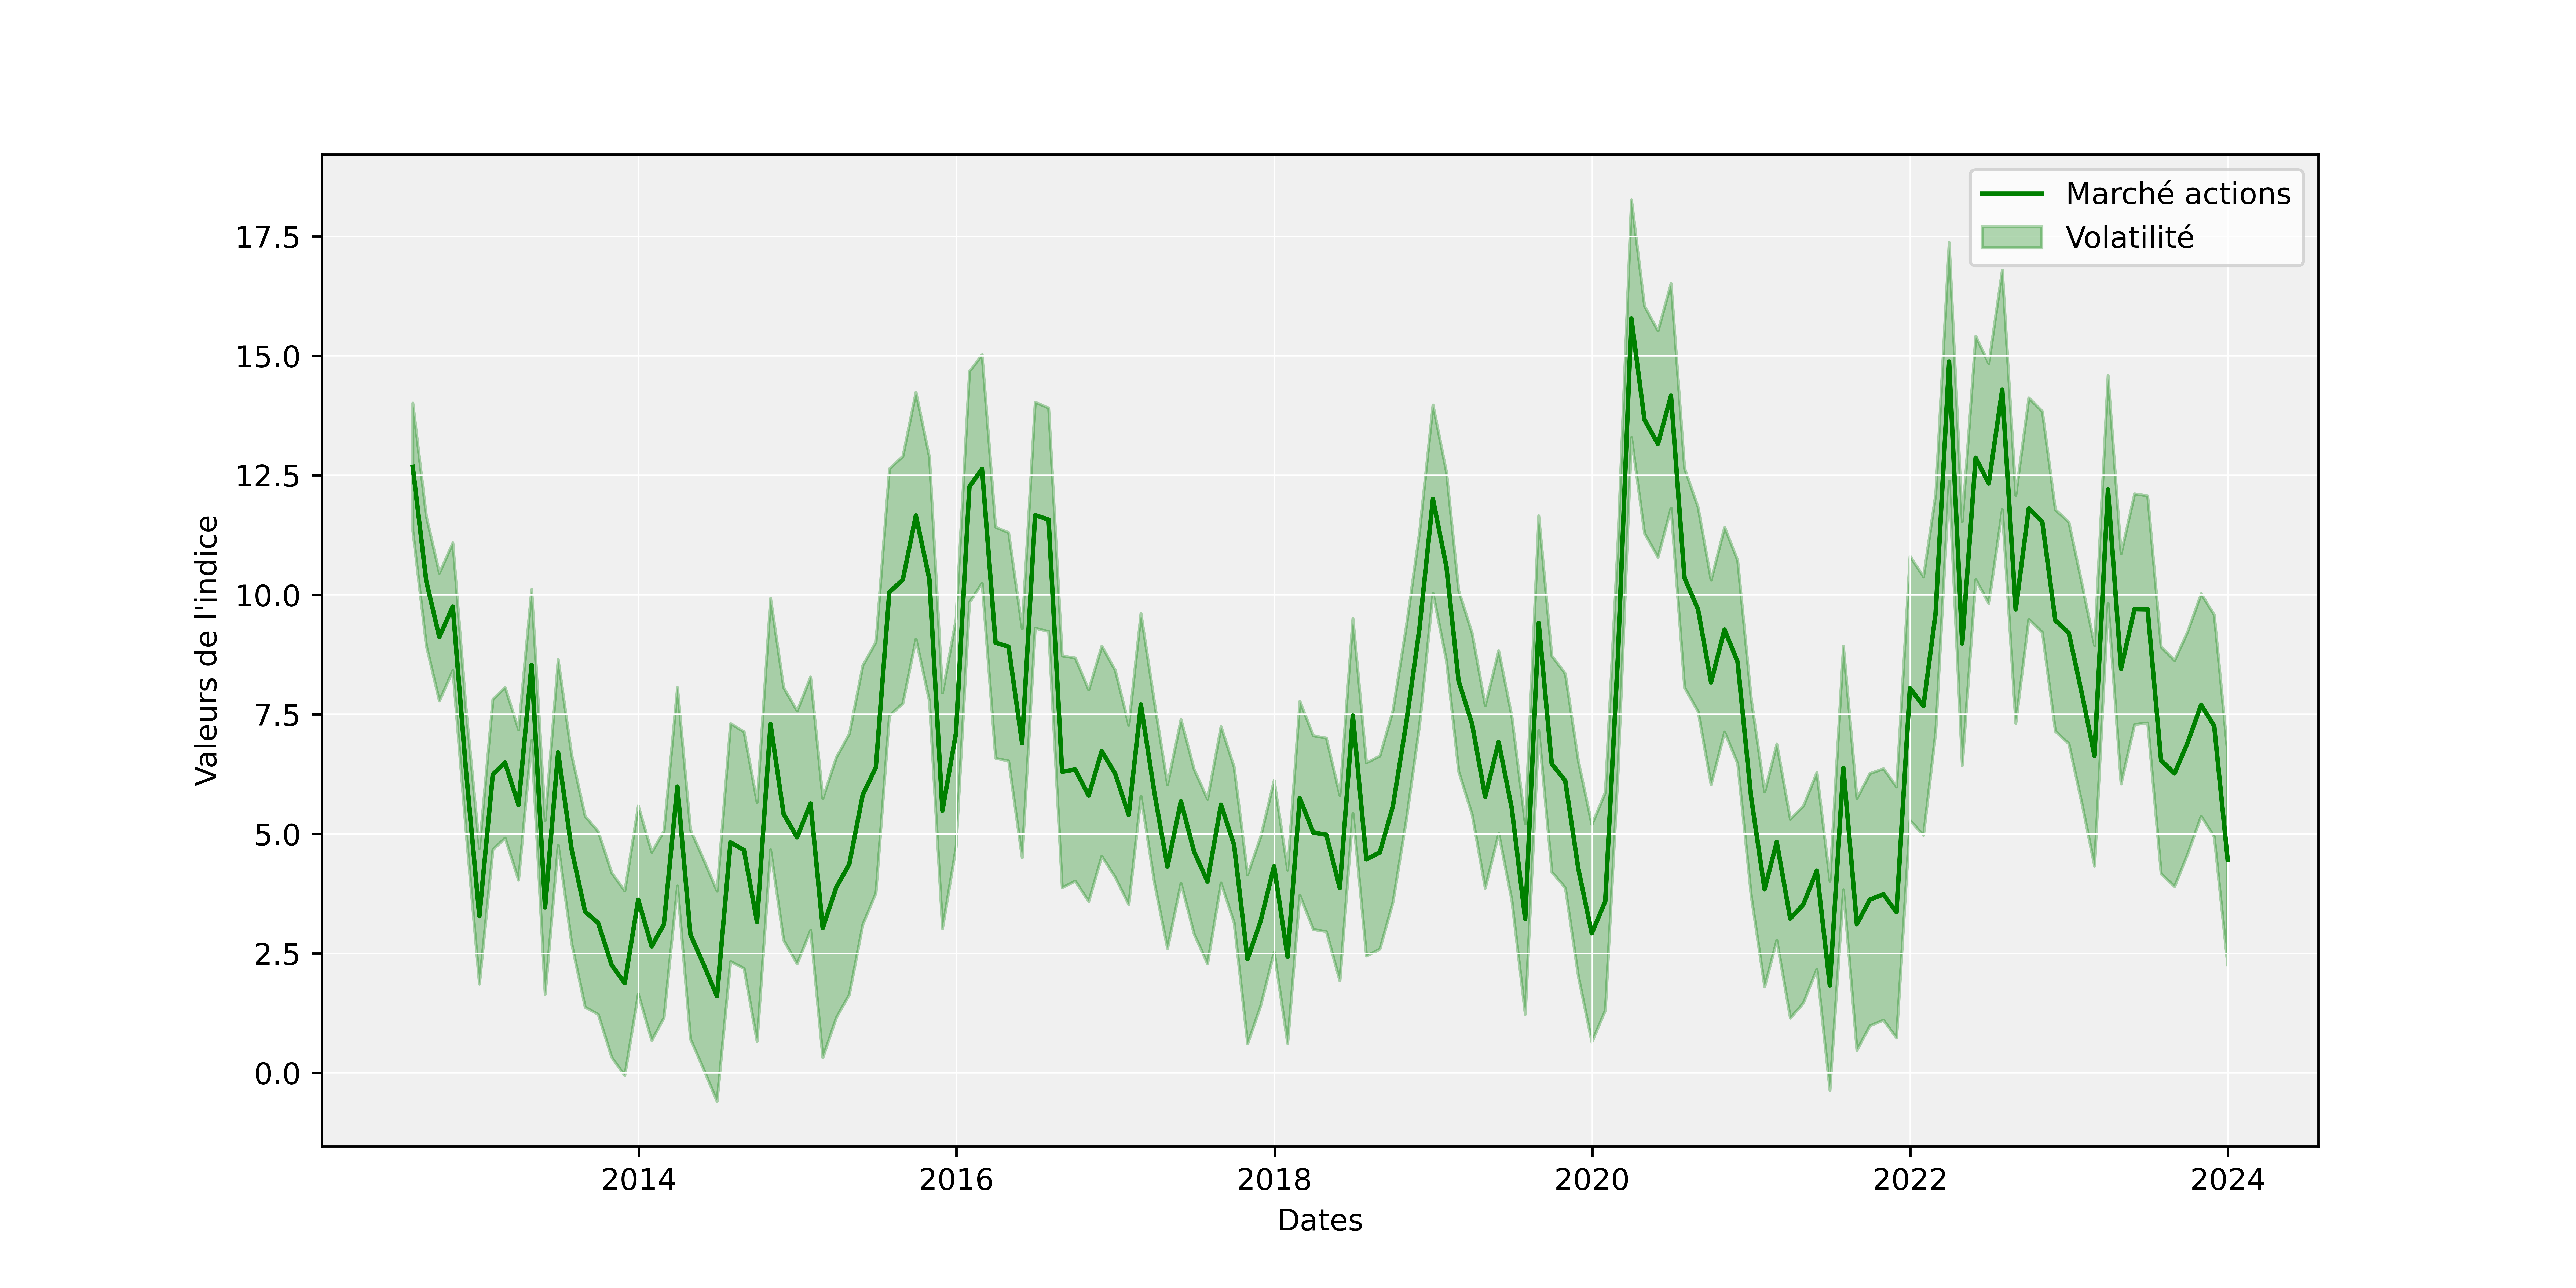
\includegraphics[width=1\linewidth]{figures/sous_indicateurs_equity_stress_equity.png}
    \caption{Stress sur le marché actions et volatilité associée entre janvier 2005 et décembre 2024.}
    \label{fig:enter-label}
\end{figure}

La volatilité observée sur le marché des actions suggère que les investisseurs réagissent fortement aux événements qui affectent la confiance dans les entreprises et l’économie en général. Les pics de volatilité élevés, particulièrement en 2008 et 2020, indiquent que les actions subissent des ajustements massifs des portefeuilles des investisseurs, souvent en raison de ventes paniquées ou de changements rapides dans les perspectives économiques.\\

En ce qui concerne le marché monétaire, cela montre des variations plus modérées par rapport aux autres marchés. Bien qu’il y ait des pics de stress, notamment autour des crises financières majeures, les valeurs de l'indicateur restent globalement plus stables. Cela reflète la nature plus régulée et contrôlée du marché monétaire, où les banques centrales interviennent régulièrement pour stabiliser les conditions de liquidité. Il est possible d'observer des pics importants autour de 2008 et un autre vers 2012, correspondant à la crise de la dette souveraine en Europe, ainsi que de légères hausses durant d'autres périodes de tension comme la crise de 2020. Cependant, contrairement au marché des actions, le marché monétaire retourne rapidement à des niveaux de stress plus bas après ces périodes de tension. Cela montre une capacité de stabilisation plus rapide dans ce segment du marché.

\begin{figure}[H]
    \centering
    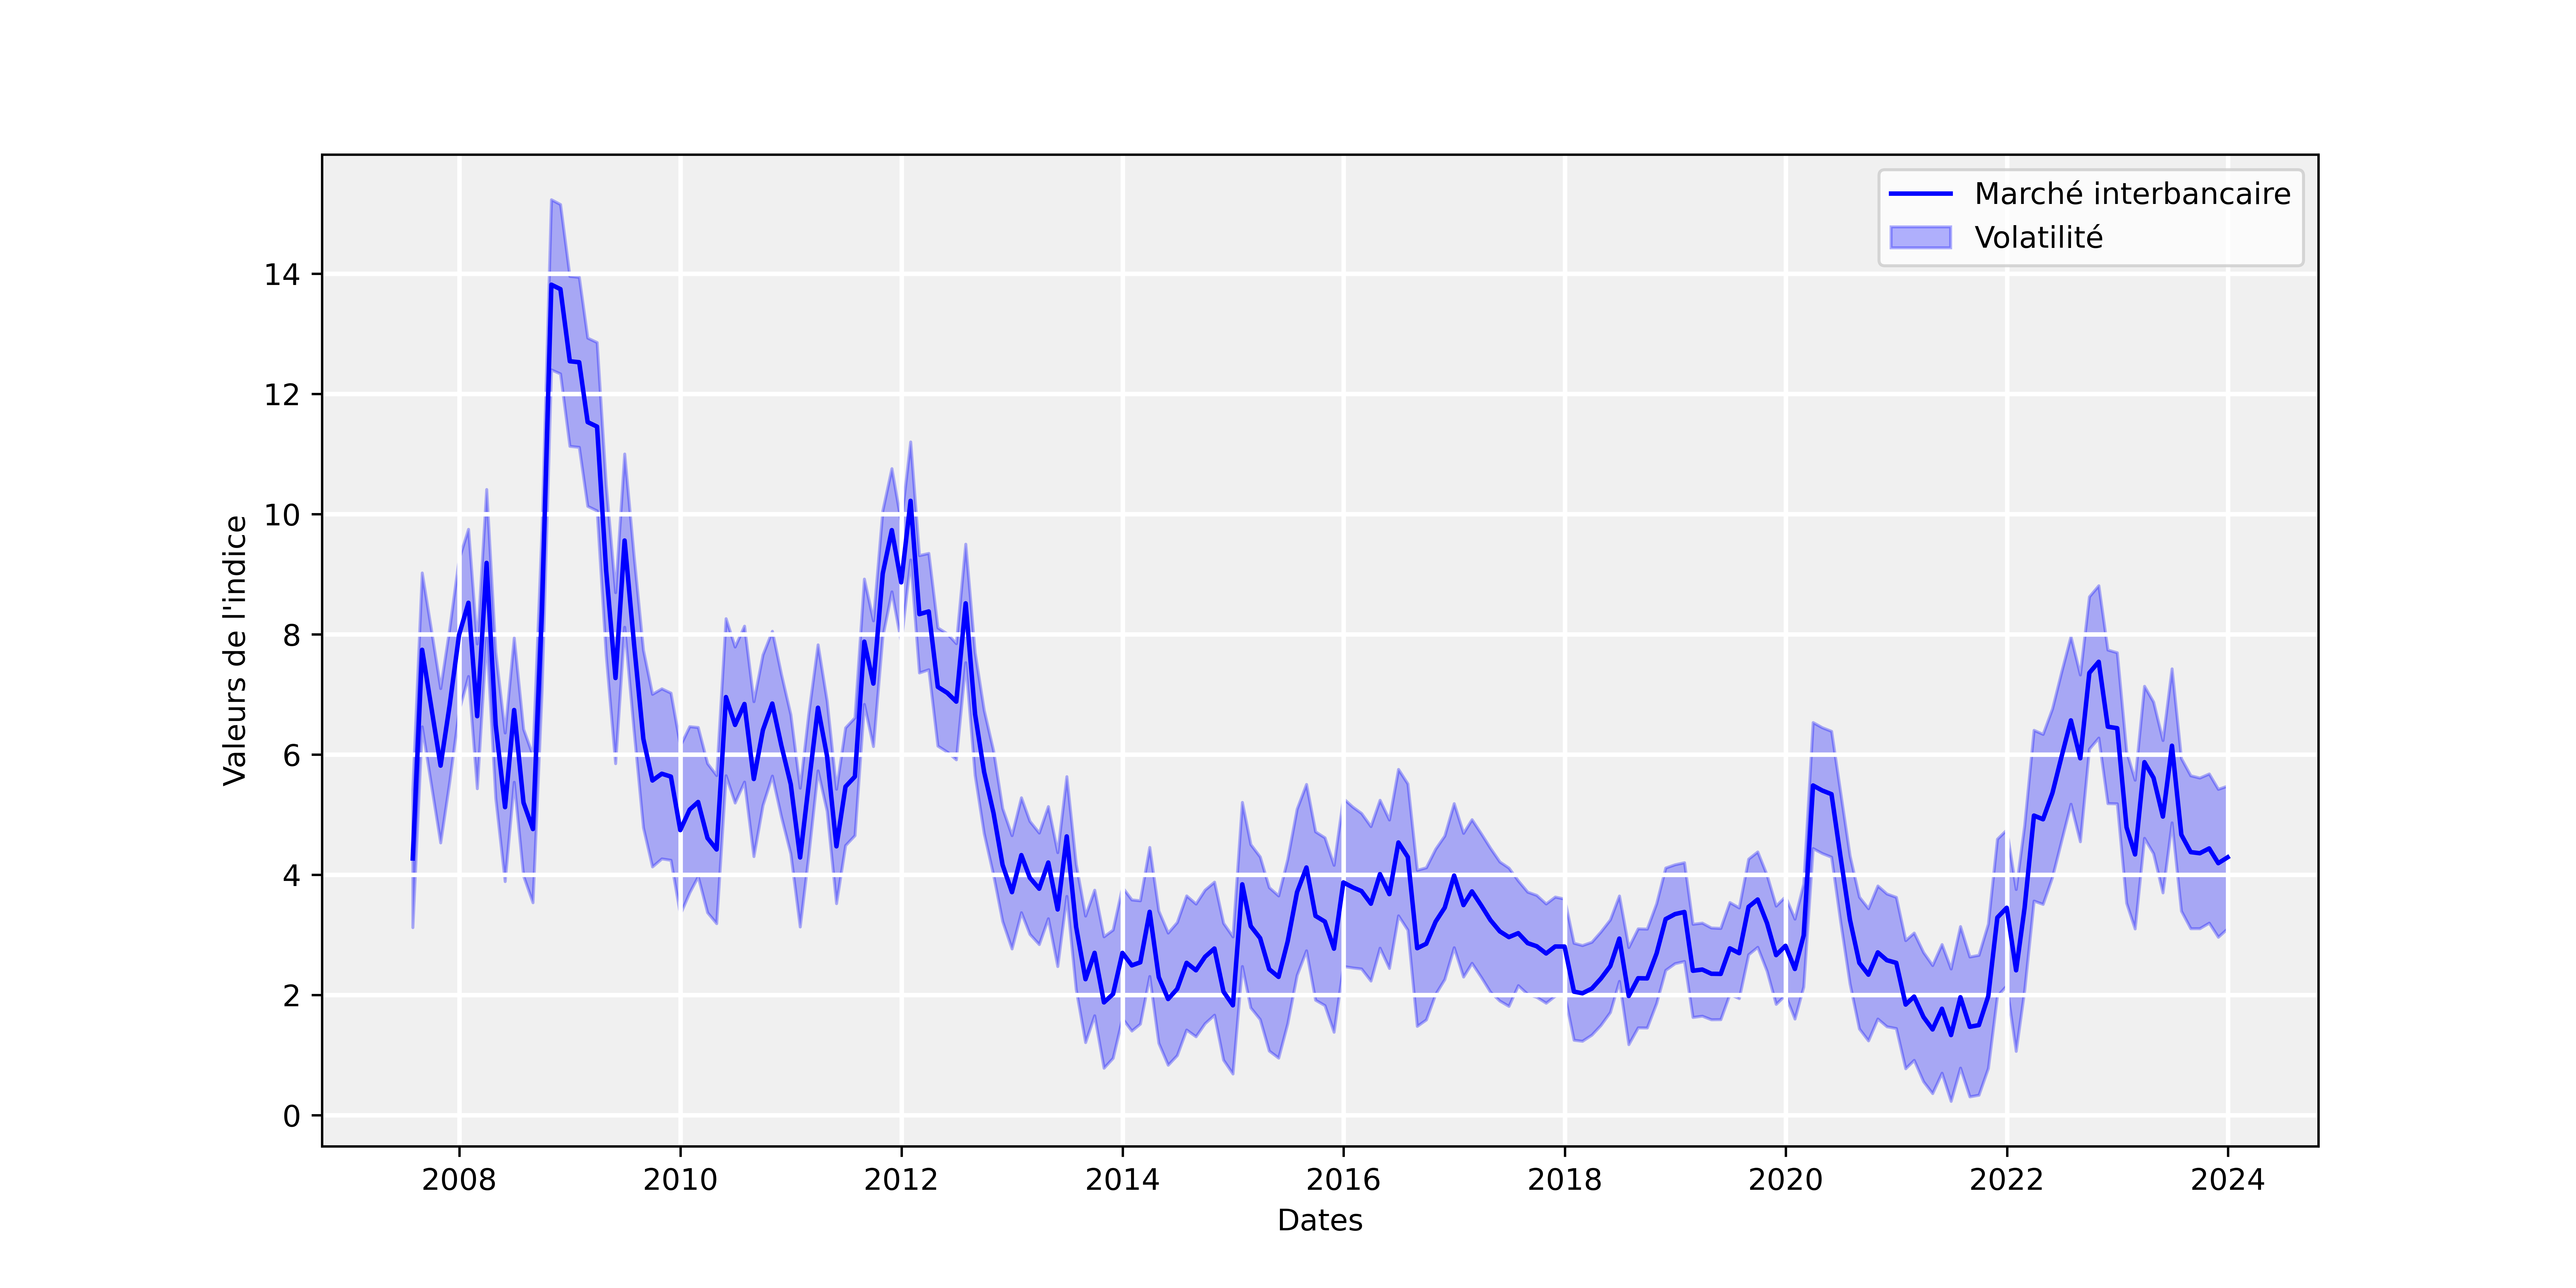
\includegraphics[width=1\linewidth]{figures/sous_indicateurs_stress_imm.png}
    \caption{Stress sur le marché monétaire et volatilité associée entre janvier 2005 et décembre 2024.}
    \label{fig:enter-label}
\end{figure}

La volatilité modérée associée au stress sur le marché monétaire, par rapport au marché des actions, est en partie due à la capacité des banques centrales à stabiliser ce marché via leurs outils de politique monétaire. Les pics de volatilité, en particulier en 2008 et 2011, sont le reflet des périodes où les banques hésitent à se prêter mutuellement, indiquant un risque accru de crise de liquidité. Cependant, après les interventions des régulateurs, la volatilité diminue rapidement, témoignant de la résilience de ce marché.\\

Enfin, le marché des changes est globalement le moins stressé parmi les trois segments, comme en témoignent les niveaux relativement bas de la courbe rouge. Cependant, ce marché montre également des épisodes de stress ponctuels, en particulier autour de 2008 et 2010-2012, ainsi que quelques augmentations notables dans les années plus récentes (vers 2020). La nature décentralisée et liquide du marché des changes lui permet de mieux absorber les chocs, bien que des périodes de forte volatilité, notamment causées par les fluctuations des taux de change et les crises monétaires, entraînent des pics soudains. Le stress sur ce marché semble être plus transitoire et moins soutenu que sur le marché des actions, où les tensions persistent souvent sur une plus longue période.

\begin{figure}[H]
    \centering
    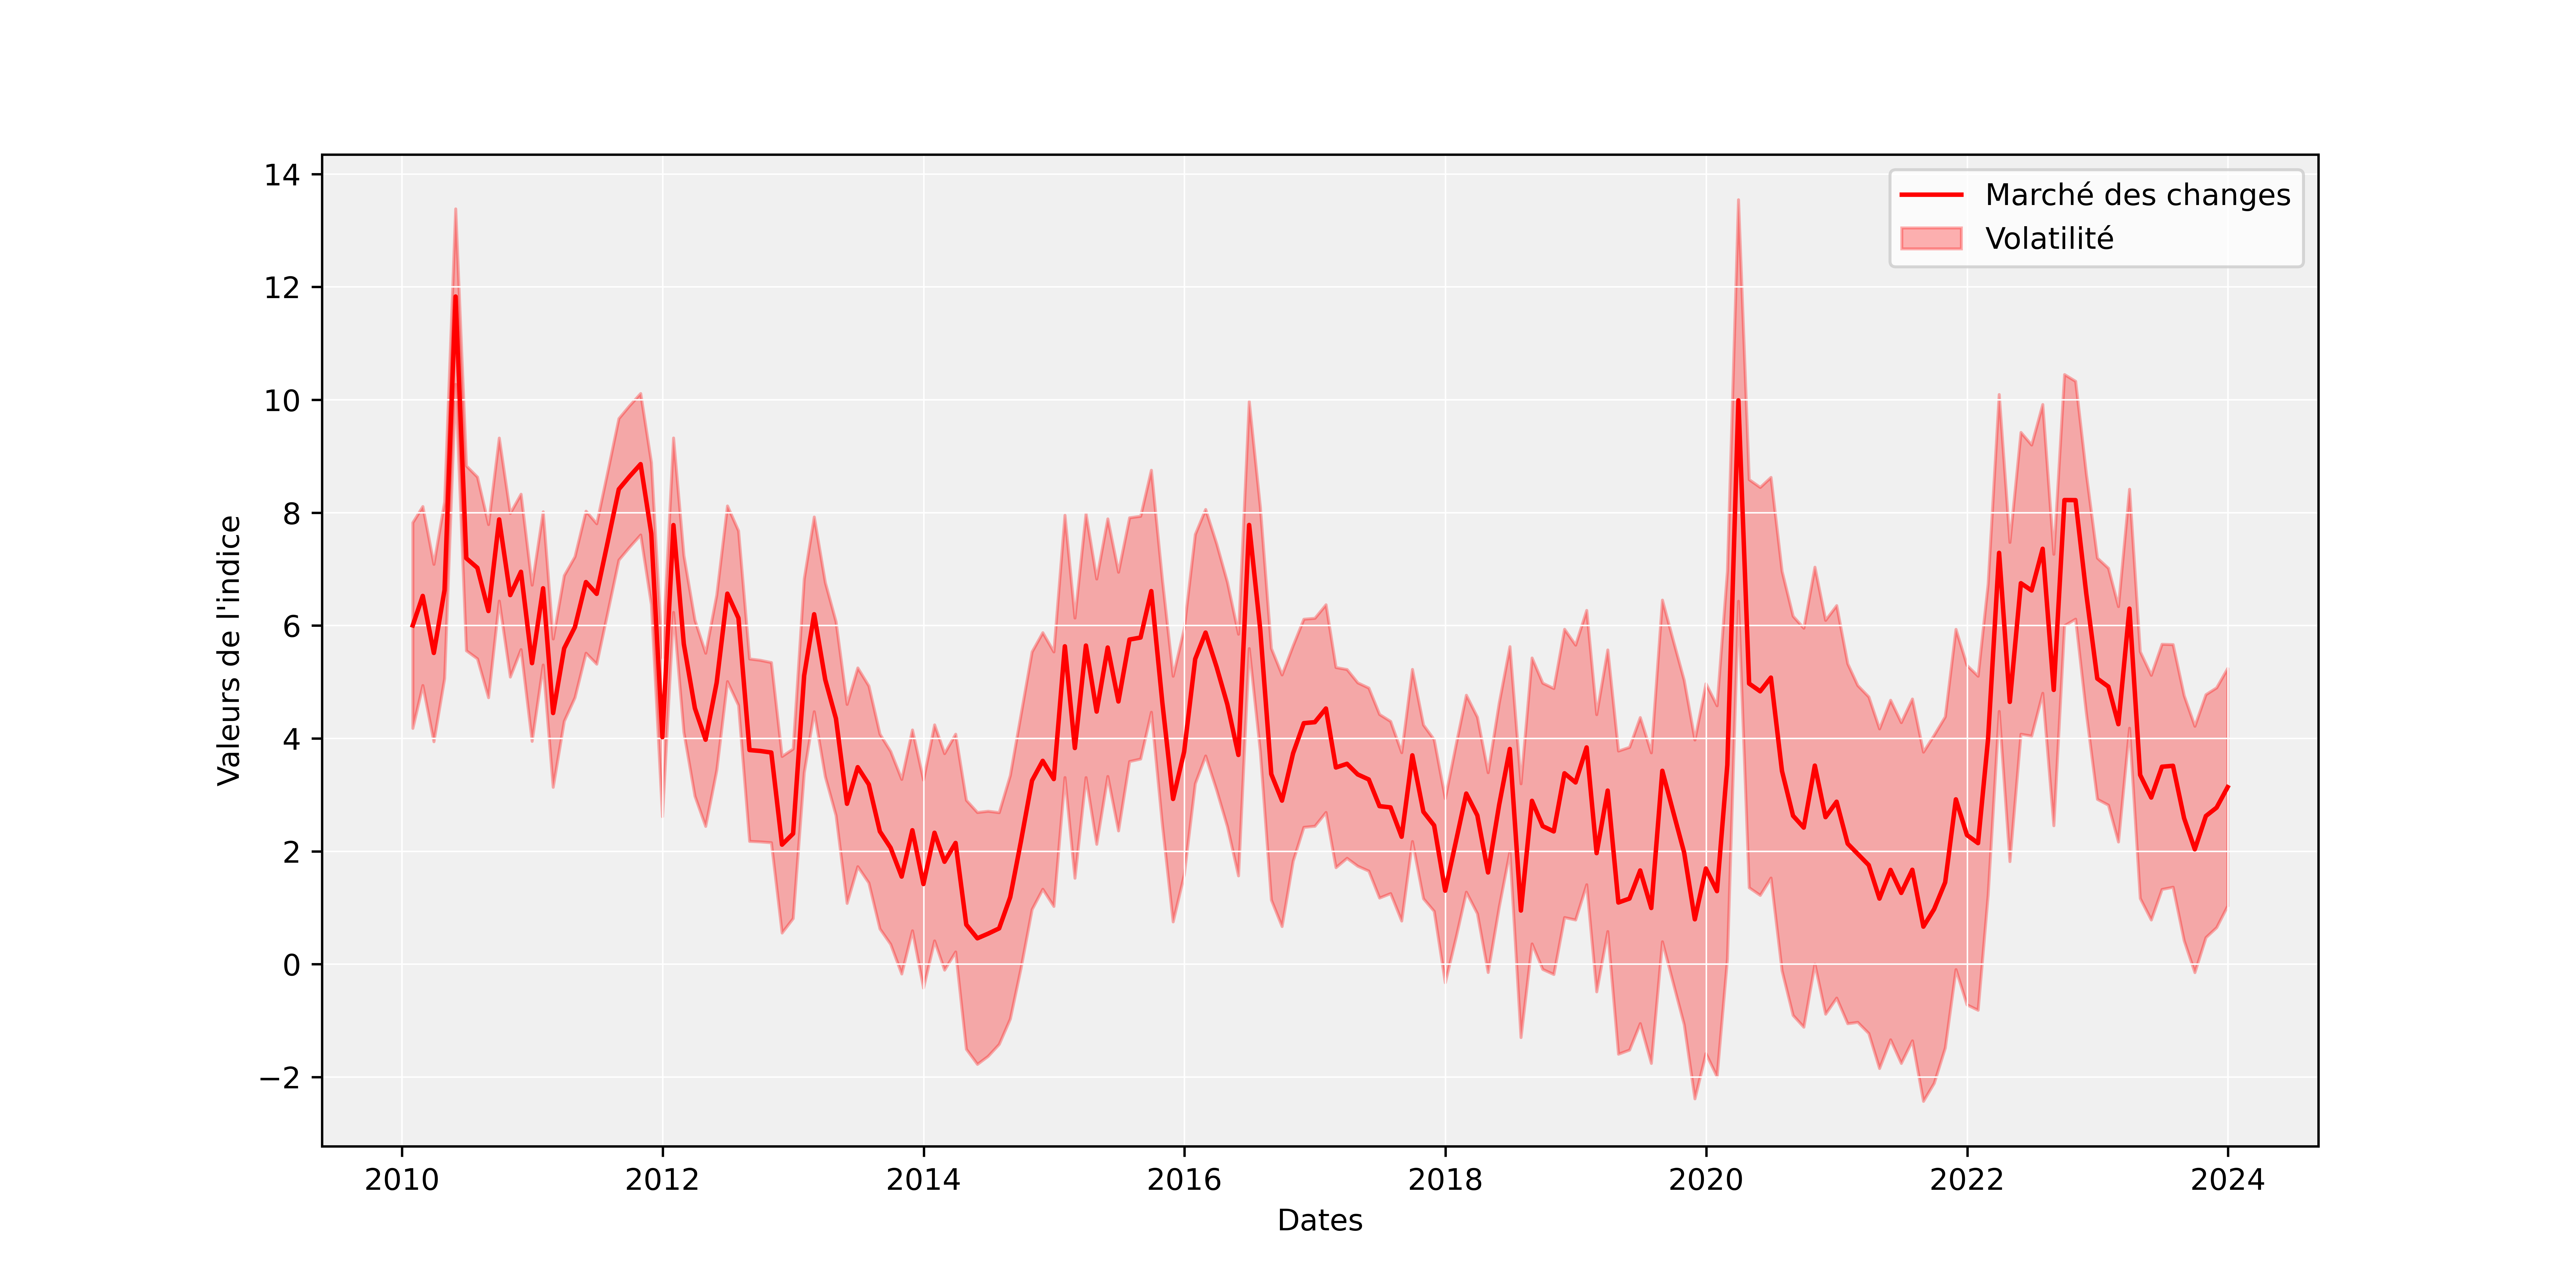
\includegraphics[width=1\linewidth]{figures/sous_indicateurs_forex_stress_forex.png}
    \caption{Stress sur le marché des changes et volatilité associée entre janvier 2005 et décembre 2024.}
    \label{fig:enter-label}
\end{figure}

La volatilité, qui accompagne les hausses de stress, est particulièrement importante autour de ces périodes. Les fluctuations observées en 2020 peuvent être attribuées aux mouvements des taux de change lors de la pandémie, ainsi qu'à la réponse des banques centrales à travers des ajustements des taux d'intérêt et des mesures non conventionnelles. Cependant, même si des périodes de stress apparaissent, le marché des changes tend à revenir à des niveaux de stress modérés sur le long terme, reflétant sa capacité à absorber les chocs grâce à sa liquidité élevée et à son caractère global.\\

En somme, l'interconnexion entre ces trois indicateurs de stress est bien visible. Lors des grandes crises financières, comme celle de 2008, on observe des pics simultanés dans les trois indicateurs, ce qui reflète un stress systémique à travers plusieurs segments financiers. Cependant, chaque marché semble réagir différemment en fonction de sa structure et de sa régulation. Le marché des actions tend à subir des chocs plus fréquents et plus sévères, tandis que le marché des changes montre une capacité à absorber les chocs avec des variations moins marquées. Le marché monétaire, quant à lui, présente une stabilité relative, malgré des tensions durant les périodes de crise.\\

Cette analyse démontre l'importance de surveiller l'évolution simultanée des sous-indicateurs de stress pour comprendre comment les tensions dans un segment peuvent se propager aux autres, exacerbant ainsi les crises financières. Après avoir effectué une analyse graphique des sous-indicateurs de stress pour les trois principaux segments financiers, l'analyse des statistiques descriptives va être mené. Cette approche permettra de mieux comprendre la distribution et les caractéristiques des différents indicateurs de stress en quantifiant leur tendance centrale, leur dispersion.

\begin{table}[H]
    \centering
    \sffamily
    \scalebox{0.9}{\begin{tabular}{lccccccc}
        \toprule
        \textbf{Indicateurs} & \textbf{Moyenne} & \textbf{Médiane} & \textbf{Maximum} & \textbf{Minimum} & \textbf{Écart-type} & \textbf{Skewness} & \textbf{Kurtosis} \\
        \midrule
        IMM      & 4.39  & 3.68  & 13.82  & 1.33  & 2.38  & 1.45  & 5.35  \\
        FOREX    & 4.19  & 3.52  & 13.52  & 0.46  & 2.65  & 1.09  & 4.07  \\
        EQUITY   & 8.02  & 6.91  & 21.31  & 1.56  & 4.56  & 0.68  & 2.64  \\
        \bottomrule
\end{tabular}


}
    \caption{Statistiques descriptives.}
    \label{fig:statsdescriptives}
\end{table}

L'analyse des moyennes montre que l'indicateur de stress sur le marché des actions  présente la valeur moyenne la plus élevée avec 8.02, suivie par les marchés interbancaire et des changes avec des moyennes respectives de 4.39 et 4.19. Cela suggère que, dans l'ensemble, le marché des actions tend à subir un stress plus important que les marchés des changes et interbancaire. En observant les valeurs médianes, il est possible de voir que le marché des actions affiche également la valeur médiane la plus élevée (6.91), ce qui renforce l'idée que ce marché est plus fréquemment sujet à des périodes de stress élevé. Les marchés interbancaire et des changes ont des valeurs médianes plus proches de leur moyenne, respectivement à 3.68 et 3.52, ce qui indique une distribution des données plus symétrique, bien que des périodes de stress aigu existent.\\

Les valeurs maximales et minimales montrent que marché des actions a connu des pics de stress beaucoup plus élevés, avec une valeur maximale de 21.31, contre 13.82 pour l'IMM et 13.52 pour le FOREX. De plus, les valeurs minimales montrent que le marché des changes a subi des périodes de stress très faibles avec une valeur minimale de 0.46, beaucoup plus basse que celles observées sur les marchés interbancaire (1.33) et des actions (1.56). Cela suggère que le marché des changes est potentiellement plus volatil avec des périodes de très faible stress ainsi que des pics de stress relativement élevés.\\

L'écart-type permet de mesurer la dispersion des données autour de la moyenne, il est aussi une mesure de la volatilité. L'indicateur de stress du marché des actions présente une dispersion plus large (4.56), indiquant une plus grande volatilité des niveaux de stress par rapport aux autres marchés. Le FOREX montre également une volatilité non négligeable avec un écart-type de 2.65, tandis que l'IMM affiche la plus faible volatilité avec 2.38.\\

En examinant les coefficients d'asymétrie, tous les indicateurs présentent une asymétrie positive, ce qui signifie que les périodes de stress extrême sont plus fréquentes du côté des valeurs élevées. Le marché interbancaire présente la plus forte asymétrie (1.45), ce qui indique que ce marché connaît des épisodes de stress élevé relativement rares mais intenses. Le FOREX est également assez asymétrique avec une valeur de 1.09, tandis que le marché des actions présente une asymétrie plus modérée avec un coefficient de 0.68. Enfin, les coefficients de kurtosis montrent des informations sur la forme de la distribution des stress. Le marché interbancaire présente une kurtosis de 5.35, ce qui indique une distribution leptokurtique, caractérisée par des extrêmes plus fréquents et des périodes de stress aigu prononcées. Le FOREX affiche également une kurtosis élevée à 4.07, tandis que le marché des actions présente une distribution plus aplatie (2.64), indiquant une distribution plus proche de la normale.\\

Cela montre donc que le marché des actions tend à subir un stress plus élevé et plus volatil que les marchés des changes et interbancaire. Cependant, les périodes de stress intense sur le marché interbancaire se caractérisent par des épisodes plus rares mais plus extrêmes, comme le montrent ses valeurs de skewness et de kurtosis.

\subsection{L'interconnexion et la contagion des sous-indicateurs étudiés}

Pour comprendre pleinement les interconnexions et les mécanismes de contagion entre le sous-indicateur de stress sur le marché des actions, des changes et le marché monétaire, il faut  reconnaître comment ces segments, qui forment des piliers du système financier, interagissent dans une dynamique systémique. La nature interdépendante de ces marchés signifie que des tensions dans l’un peuvent rapidement se propager aux autres, amplifiant ainsi le risque systémique. C’est précisément cette complexité et cette interdépendance qui justifient l’importance de construire des indicateurs de stress systémique comme le \textit{CISS}, afin de surveiller, anticiper et réagir aux crises qui pourraient perturber l’économie.\\

Premièrement, les interconnexions seront étudiées avant d'étudier les mécanismes de contagion afin de discuter dans un troisième temps les implications macroprudentielles et monétaires.\\

\subsubsection{Les interconnexions entre les trois sous-indicateurs}

Les sous-indicateurs de stress des marchés actions, des changes et monétaires sont fortement interconnectés. Cette interdépendance résulte de flux financiers partagés, de comportements synchronisés des investisseurs, et des politiques monétaires et fiscales qui affectent simultanément ces segments. En période de crise, ces interconnexions deviennent plus visibles, car les acteurs du marché ajustent rapidement leurs positions en fonction des tensions apparentes dans d'autres segments.\\

Tout d'abord, le sous-indicateur de stress sur le marché des actions reflète la volatilité et les pertes cumulées sur les principaux indices boursiers, notamment ceux des entreprises non financières. En période de stress, une volatilité accrue sur le marché des actions signale une incertitude grandissante quant à la rentabilité des entreprises, à la stabilité économique globale et au comportement des investisseurs. Ces derniers, lorsqu'ils perçoivent des risques élevés sur le marché des actions, peuvent chercher à réallouer leurs portefeuilles vers des actifs jugés plus sûrs, comme les obligations d'État ou les monnaies refuges. Ce phénomène de réallocation peut alors affecter d’autres segments financiers, créant un effet de contagion. Par exemple, une baisse généralisée des indices boursiers peut pousser les investisseurs à vendre des actions en masse, ce qui augmente la pression vendeuse sur le marché des changes lorsque ces ventes concernent des entreprises exposées aux fluctuations des devises.\\

Ensuite, le FOREX est un canal fondamental par lequel les politiques monétaires, les flux de capitaux et les événements macroéconomiques influencent directement les autres segments financiers. Le sous-indicateur de stress du FOREX capture la volatilité des taux de change et les tensions qui en découlent. En période de forte incertitude, une dépréciation rapide d'une devise, souvent provoquée par des déséquilibres économiques ou des ajustements des taux d’intérêt, peut entraîner une volatilité accrue sur ce marché. Cela affecte directement les entreprises multinationales, dont la rentabilité est liée aux variations des taux de change. Par conséquent, une volatilité sur le stress du marché des changes affecte la compétitivité internationale des entreprises cotées, provoquant une instabilité sur le stress du marché des actions. Cette interaction souligne l'importance des indicateurs composites, comme le CISS, qui permettent de surveiller simultanément plusieurs segments et d'évaluer l'impact global d'une crise dans l'un d'eux.\\

Enfin, le marché monétaire est essentiel pour garantir la liquidité à court terme et le financement des banques et autres intermédiaires financiers. Le sous-indicateur de stress sur ce marché suit la volatilité des taux interbancaires, les spreads entre les obligations d'État et les taux interbancaires, ainsi que le recours aux facilités de liquidité d'urgence fournies par les banques centrales. Une crise de liquidité dans ce segment provoque des effets immédiats sur les autres marchés, car les banques et autres institutions financières sont contraintes de liquider des actifs, y compris des actions et des devises, pour générer des liquidités. Cela aggrave les tensions sur les marchés des actions et des changes, en augmentant la pression vendeuse et, par conséquent, la volatilité sur l'ensemble du système financier. La surveillance du marché monétaire est donc primordiale pour détecter et prévenir les crises de liquidité pouvant rapidement se propager à d'autres segments.

\subsubsection{Mécanismes de contagion entre les trois sous-indicateurs}

Les interconnexions observées entre ces trois sous-indicateurs de stress sont renforcées par des mécanismes de contagion, qui rendent les marchés particulièrement vulnérables aux chocs extérieurs. Ces mécanismes s'intensifient surtout en période de crise, lorsque le stress dans un segment localisé s'étend rapidement aux autres, créant un effet domino.\\

Un première peut être que le marché monétaire est un canal principal de transmission des chocs financiers, car il assure la liquidité nécessaire au bon fonctionnement des institutions financières. En période de crise, lorsque les taux interbancaires augmentent de manière significative, les institutions financières se retrouvent en situation de tension de liquidité. Pour compenser, elles vendent des actifs, notamment des actions et des devises, amplifiant ainsi la volatilité sur ces marchés. Ce cercle vicieux où la vente massive d’actions exacerbe la baisse des cours, alimente les incertitudes et accroît les tensions sur les autres marchés, démontre l’importance d’un suivi étroit des tensions de liquidité. Le stress monétaire peut également affecter le marché des changes, car les banques rapatrient des capitaux ou ajustent leurs positions en devises pour faire face à leurs besoins de liquidité, amplifiant la volatilité sur le FOREX.\\

Il est possible d'évoquer les stratégies d'arbitrage, qui consistent à exploiter les différences de prix entre les actifs, constituent un autre mécanisme de contagion important. Lorsqu'une volatilité significative apparaît sur le marché des actions, les investisseurs ajustent souvent leurs positions sur le marché des changes pour couvrir les risques de change, ou pour spéculer sur les variations futures des devises. Cela entraîne une volatilité accrue sur le FOREX, aggravant les tensions dans ce segment. Par ailleurs, lorsque les investisseurs cherchent à limiter leurs pertes sur un marché, ils réallouent leurs portefeuilles vers d'autres marchés plus stables, ce qui exerce une pression supplémentaire sur l'ensemble du système financier.\\

Aussi, lors des périodes de crises financières, les investisseurs tentent généralement de protéger leur capital en transférant leurs fonds vers des actifs jugés plus sûrs, tels que les obligations d'État ou les devises stables, comme le dollar américain. Ce mouvement, appelé "fuite vers la qualité", affecte directement le marché des changes, car les devises refuges connaissent une hausse de la demande, entraînant des fluctuations importantes des taux de change. Ce phénomène a des répercussions sur les marchés actions, en particulier pour les entreprises exportatrices, dont les revenus dépendent des variations de change. En effet, une forte appréciation des devises refuges peut rendre les exportations plus coûteuses, réduisant ainsi la compétitivité des entreprises sur les marchés internationaux et aggravant les tensions sur les marchés actions.

\subsubsection{Rôle des politiques monétaires et macroprudentielles}

L’un des principaux objectifs de la BCE et des régulateurs financiers est de maintenir la stabilité financière tout en garantissant une inflation maîtrisée. Dans ce contexte, les sous-indicateurs de stress des marchés des actions, des changes et monétaires, ainsi que le CISS, jouent un rôle clé dans la surveillance du système financier et dans l'orientation des politiques monétaires et macroprudentielles. Ces indicateurs fournissent des signaux précoces qui permettent d’ajuster les politiques en fonction des tensions observées sur les différents marchés.\\

L'intérêt de construire des indicateurs comme le CISS réside dans leur capacité à capturer les interconnexions entre les différents segments financiers et à identifier les périodes où le stress est suffisamment élevé pour entraîner une contagion systémique. Le CISS offre une vision d’ensemble des risques systémiques en agrégant les sous-indicateurs des marchés actions, des changes et monétaires, tout en tenant compte de leurs corrélations dynamiques. Cela permet aux décideurs politiques de mieux anticiper les crises et d'intervenir de manière préventive pour éviter une amplification des tensions.\\

Par exemple, en surveillant l'évolution du CISS, la BCE peut évaluer à quel moment les tensions sur un segment donné, comme le marché monétaire, deviennent suffisamment importantes pour justifier une intervention. Cela pourrait inclure des injections de liquidités sur le marché monétaire ou un assouplissement des taux d'intérêt pour soutenir les banques en période de tension. De plus, en ajustant les exigences de fonds propres des banques ou en mettant en place des coussins de capital anticrises, la BCE peut renforcer la résilience du système bancaire et réduire la contagion potentielle des crises. Ainsi, l’analyse des indicateurs de stress systémique permet non seulement d'identifier les moments critiques où une intervention est nécessaire, mais aussi d'adapter les outils macroprudentiels pour prévenir des crises futures.\\

L’étude des interactions entre les différents segments du système financier, ainsi que l’élaboration d’indicateurs comme le CISS, mettent en évidence la complexité et l’interdépendance des marchés financiers modernes. À travers une analyse approfondie des marchés des actions, des changes et monétaires, cette partie a montré comment les tensions systémiques se développent et se propagent, illustrant ainsi la nécessité d’une surveillance holistique et proactive. L’approche intégrée du CISS, qui combine des indicateurs spécifiques avec des corrélations dynamiques, représente un outil clé pour évaluer les risques systémiques et guider les politiques monétaires et macroprudentielles.\\

Les mécanismes de contagion, tels que la propagation via la liquidité ou les ajustements de portefeuilles, soulignent l’importance de comprendre les interactions entre segments pour anticiper les crises systémiques. En outre, l’analyse des sous-indicateurs a révélé que chaque marché, bien que distinct dans sa structure et ses dynamiques, contribue de manière significative à l’évaluation globale du stress financier. Les marchés des actions se caractérisent par leur volatilité accrue, les marchés des changes par leur résilience, et les marchés monétaires par leur rôle critique dans la fourniture de liquidités, illustrant ainsi la complémentarité des segments.\\

Cette partie a également mis en lumière l’utilité pratique du CISS pour les régulateurs et les décideurs politiques, en leur fournissant des outils pour surveiller et stabiliser le système financier. En anticipant les périodes de stress systémique et en ajustant les politiques en conséquence, les autorités peuvent limiter l’impact des crises financières sur l’économie réelle, protégeant ainsi la croissance économique et la stabilité sociale.\\

Après avoir établi les fondements théoriques et méthodologiques du CISS, l’analyse se tourne désormais vers la méthodologie économétrique utlisée dans ce projet. Cette transition est nécessaire pour quantifier les relations dynamiques entre les sous-indicateurs de stress, mesurer les interactions entre les marchés et évaluer empiriquement les mécanismes de contagion identifiés. La partie économétrique s’appuiera sur des modèles non-linéaires adaptés, notamment des modèles MS-VAR et NARDL.

\end{sloppypar}


\newpage
\section{Modèles non-linéaires à changement de régimes markoviens et asymétriques}

\begin{sloppypar}
Ce paragraphe présente les fondements théoriques des modèles économétriques avancés appliqués à l’analyse des interactions entre trois sous-indicateurs du CISS étudiés.\\

Le premier sous-paragraphe commence par une introduction aux chaînes de Markov. Les chaînes de Markov, initialement introduites par Andrey Markov en 1906, ont été développées pour étudier les dépendances entre événements dans des processus aléatoires. Markov a appliqué cette théorie à des séquences de lettres dans des textes littéraires, démontrant ainsi qu'il est possible de modéliser des systèmes où l'état futur dépend uniquement de l'état présent, et non de l'ensemble des états passés. Depuis lors, ces chaînes sont devenues un outil très utilisé en mathématiques appliquées, économie et physique, pour modéliser des phénomènes de changements de régimes.\\

Le second sous-paragraphe approfondit la spécification du modèle Markov Switching-VAR en expliquant ses typologies et les méthodologies associées, telles que la décomposition de Cholesky, les moments conditionnels et les réponses aux chocs. Les typologies incluent des modèles à variances constantes ou variables selon les régimes, tandis que les moments conditionnels permettent d’étudier la dynamique des réponses des variables aux chocs exogènes dans chaque régime. La décomposition de Cholesky est utilisée pour identifier les chocs structurels dans les séries temporelles.
Enfin, dans ce sous-paragraphe, il est présenté les méthodes d'estimation et de filtrage avec l'algorithme de Hamilton pour illustrer l’ajustement des modèles dans un cadre multirégime. Cet algorithme est crucial pour estimer les probabilités ex-post des régimes et les paramètres du modèle, en maximisant la vraisemblance jointe des observations dans un cadre non-linéaire.\\

Le dernier sous-paragraphe introduit le modèle univarié NARDL pour analyser les dynamiques non-linéaires asymétriques. Ce modèle permet de capturer les effets asymétriques des variations positives et négatives d’une variable explicative sur une variable dépendante. Il est particulièrement adapté pour analyser des phénomènes économiques où les ajustements aux chocs diffèrent selon leur direction, offrant ainsi une perspective complémentaire au MS-VAR dans le cadre des sous-indicateurs du CISS.

\subsection{Chaîne de Markov}

Les chaînes de Markov offrent un cadre mathématique pour modéliser les processus stochastiques où l’évolution d’un système est latent. En économétrie, ce concept se révèle particulièrement utile pour décrire des phénomènes économiques présentant des changements d’état abrupts ou des transitions entre différents régimes. Ce sous-paragraphe introduit les chaînes de Markov en explorant leurs caractéristiques fondamentales, telles que la relation de Chapman-Kolmogorov, qui exprime la probabilité de transition entre états sur plusieurs étapes, ainsi que la classification des états, qui permet de distinguer entre les états récurrents et transients. La périodicité et les lois de probabilité stationnaires viennent compléter cette étude, fournissant ainsi les bases nécessaires pour appliquer les chaînes de Markov dans des modèles utilisés lors de ce projet qui est le modèle Markov Switching-VAR.

\subsubsection{Généralités sur les chaînes de Markov}
Afin d'illustrer cette partie, la présentation de la notion de Chaînes de Markov est amplement tirée du cours de préparation à l'agrégation de mathématiques de l'Université de Bordeaux 1 de \cite[2013]{Ruch et Chabanol}.\\

Les chaînes de Markov constituent un des exemples les plus simples de suites de variables aléatoires $(X_n)$. 
Les variables $(X_n)$ sont à valeurs dans un ensemble $E$ appelé espace d’état. 
Certaines chaînes de Markov sont à espace d’états continu, mais il ne sera pas abordé leur étude ici. 
Seules les chaînes à espace d’états fini ou dénombrable. 
Dans toute la suite, $E$ sera donc un ensemble fini ou dénombrable ($\mathbb{N}$ ou un sous-ensemble), que l’on munira de la tribu de toutes ses parties. 

\begin{tcolorbox}[colback=blue!5!white,colframe=blue!75!black,title=Définition]
Une suite $(X_n)_{n \geq 0}$ de variables aléatoires à valeurs dans un ensemble au plus dénombrable $E$ est une chaîne de Markov d’espace d’états $E$ si et seulement si pour tout $k \in \mathbb{N}$,
pour tout $(x_0,...,x_{k+1})$ dans $E$ tels que $\mathbb{P}(X_k = x_k,...,X_0 = x_0) > 0$,

\begin{equation}
\mathbb{P}(X_{k+1} = x_{k+1} \mid X_k = x_k,...,X_0 = x_0) = \mathbb{P}(X_{k+1} = x_{k+1} \mid X_k = x_k).    
\end{equation}

Cela s’écrit également

\begin{equation}
\mathcal{L}(X_{k+1} \mid X_k = x_k,...,X_0 = x_0) = \mathcal{L}(X_{k+1} \mid X_k = x_k)    
\end{equation}

pour tout $k \in \mathbb{N}$.\\

Cela signifie que seule la valeur de l'état actuel \(X_t\) influe sur la probabilité de l'état futur \(X_{t+1}\).\\
\end{tcolorbox}


La chaîne est dite homogène si il y a de plus pour tout $k \in \mathbb{N}$ et tout $x$ et $y$ dans $E$,
\begin{equation}
    \mathbb{P}(X_{k+1} = y \mid X_k = x) = \mathbb{P}(X_1 = y \mid X_0 = x)  
\end{equation}

\begin{tcolorbox}[colback=blue!5!white,colframe=blue!75!black,title=Définition]
    On appelle probabilité de transition pour aller de l’état $x$ à l’état $y$ la probabilité
    \begin{equation}
    p_{x,y} = \mathbb{P}(X_{k+1} = y \mid X_k = x) (= \mathbb{P}(X_1 = y \mid X_0 = x)).
    \end{equation}
    \end{tcolorbox}


Il est noté $\nu_0$ la loi de $X_0$ ($\nu_0(x_0) = \mathbb{P}(X_0 = x_0)$). Il est donc obtenu que pour tout $(x_0, \dots, x_n) \in E$

\begin{equation}
\mathbb{P}(X_n = x_n, \dots, X_0 = x_0) = \nu_0(x_0) \prod_{k=0}^{n-1} p_{x_k, x_{k+1}}.   
\end{equation}

En effet, 
\begin{equation}
\begin{split}
 &\mathbb{P}(X_n = x_n, \dots, X_0 = x_0) = \mathbb{P}(X_0 = x_0) \mathbb{P}(X_1 = x_1 \mid X_0 = x_0) \\
&\mathbb{P}(X_2 = x_2 \mid X_1 = x_1, X_0 = x_0) \dots \mathbb{P}(X_n = x_n \mid X_{n-1} = x_{n-1}, \dots, X_0 = x_0)\\
&= \nu(x_0) \prod_{k=0}^{n-1} p_{x_k, x_{k+1}}.
\end{split}   
\end{equation}

\begin{tcolorbox}[colback=blue!5!white,colframe=blue!75!black,title=Définition]
Il est appellé matrice de transition la matrice $\mathcal{P} = (p_{x,y})_{x,y \in E}$ :
\begin{equation}
\mathcal{P} =
\begin{pmatrix}
p_{x_0,x_0} & p_{x_0,x_1} & p_{x_0,x_2} & \cdots \\
p_{x_1,x_0} & p_{x_1,x_1} & p_{x_1,x_2} & \cdots \\
p_{x_2,x_0} & p_{x_2,x_1} & p_{x_2,x_2} & \cdots \\
\vdots & \vdots & \vdots & \ddots
\end{pmatrix}.   
\end{equation}

D'après le lemme précédent, la loi d'une chaîne de Markov est caractérisée par la loi $\nu_0$ de $X_0$ et par
sa matrice de transition.
\end{tcolorbox}

Toute matrice de transition vérifie les propriétés suivantes dérivées des définitions probabilistes :
\begin{enumerate}
    \item Pour tout couple $(x,y) \in E$, $0 \leq p_{x,y} \leq 1$ ;
    \item Pour tout $x \in E$, on a $\sum_{y \in E} p_{x,y} = 1$.
\end{enumerate}

\begin{tcolorbox}[colback=green!5!white,colframe=green!75!black,title=Proposition]
Il est identifié une probabilité $\mu$ sur $E$ et le vecteur ligne dont la $i$-ème coordonnée est
$\mu(x_i)$. Soit $(X_n)$ une chaîne de Markov de matrice de transition $P$, et soit $\nu_0$ la loi de $X_0$. Alors la loi de
$X_1$ est $\nu_1 = \nu_0 \mathcal{P}$, et pour tout entier $n$, la loi de $X_n$ est $\nu_n = \nu_0 \mathcal{P}^n$.
\end{tcolorbox}

Pour le premier point, il est établi pour tout $x_i \in E$,

\begin{equation}
\mathbb{P}(X_1 = x_i) = \sum_{x_j \in E} \mathbb{P}(X_1 = x_i \mid X_0 = x_j) \mathbb{P}(X_0 = x_j) = \sum_{x_j \in E} \nu_0(x_j) \mathcal{P}_{j,i} = (\nu_0 \mathcal{P})_i.   
\end{equation}

(en posant par convention $P(A \mid B) P(B) = 0$ si $P(B) = 0$). 
Ensuite,  il peut être procédé par récurrence. Il est à noter $(Q_n)$ la proposition $\nu_n = \nu_0 \mathcal{P}^n$. Il vient d'être prouver $Q_1$. Il reste à vérifier l’hérédité. Soit $n > 0$. Il est supposé $\nu_n = \nu_0 \mathcal{P}^n$. Alors pour tout $x_i \in E$,

\begin{equation}
   \mathbb{P}(X_{n+1} = x_i) = \sum_{x_j \in E} \mathbb{P}(X_{n+1} = x_i \mid X_n = x_j) \mathbb{P}(X_n = x_j) = \sum_{x_j \in E} \nu_n(j) \mathcal{P}_{j,i} = (\nu_0 \mathcal{P}^{n+1})_i 
\end{equation}

Ainsi, l'évolution de la loi de $X_n$ se ramène en fait à de l'algèbre linéaire. À toute matrice de transition, un graphe dirigé peut être associé, éventuellement infini. Les sommets du
graphe sont les différents états de la chaîne. Il y a une flèche, étiquetée $p_{x,y}$, entre le sommet $x$ et le
sommet $y$ si et seulement si la probabilité de transition est strictement positive : $p_{x,y} > 0$. La chaîne peut
alors s’interpréter comme une marche aléatoire sur le graphe. Cela donne par exemple pour trois régimes : 

\begin{center}
\begin{tikzpicture}[->, >=stealth', auto, semithick, node distance=4cm]

    \tikzstyle{state}=[circle,thick,draw=black,fill=gray!10,minimum size=2cm]
  
    % Nodes
    \node[state] (R1) {Régime 1};
    \node[state] (R2) [right of=R1] {Régime 2};
    \node[state] (R3) [below of=R1, xshift=2cm, yshift=-1cm] {Régime 3};
  
    % Edges
    \path (R1) edge [loop left] node{\(p_{11}\)} (R1)
              edge [bend left=20] node{\(p_{12}\)} (R2)
              edge [bend right=20] node[below left]{\(p_{13}\)} (R3)
          (R2) edge [loop right] node{\(p_{22}\)} (R2)
              edge [bend left=20] node{\(p_{21}\)} (R1)
              edge [bend left=20] node[below right]{\(p_{23}\)} (R3)
          (R3) edge [loop below] node{\(p_{33}\)} (R3)
              edge [bend right=25] node[above left]{\(p_{31}\)} (R1)
              edge [bend left=27] node[above right]{\(p_{32}\)} (R2);
  
  \end{tikzpicture}
\end{center}

\subsubsection{Relation de Chapman-Kolmogorov}

Ainsi, est appelée la propriété reliant, pour une chaîne de Markov homogène, les probabilités de transition
en $n$ étapes aux probabilités en une seule étape.\\

Il est à noter $(X_n)_{n \geq 0}$ une chaîne de Markov homogène, dont l’ensemble des états est $E$ et la matrice de transition $\mathcal{P} = (p_{i,j})_{(i,j) \in E^2}$. Pour $n \geq 0$ et $i, j \in E$, il est désigné par $p^{(n)}_{i,j}$ la probabilité, partant de l’état $i$
à l’instant $0$, d’être dans l’état $j$ à l’instant $n$; en d’autres termes on a :

\begin{equation}
 p^{(n)}_{i,j} = \mathbb{P}(X_n = j \mid X_0 = i)   
\end{equation}

La relation de Chapman-Kolmogorov qui suit peut s’interpréter en disant que “pour passer de $i$ à $j$ en
$m + n$ étapes, il a bien fallu en $m$ étapes aller de $i$ à un certain $k$, puis en $n$ étapes aller de $k$ à $j$.

\begin{tcolorbox}[colback=green!5!white,colframe=green!75!black,title=Proposition]
Pour tout $(i, j) \in E^2$ et tout couple $(m, n)$ d’entiers positifs, on a l’identité :
    
\begin{equation}
 \mathbb{P}(X_{m+n} = j \mid X_0 = i) = \sum_{k \in E} \mathbb{P}(X_m = k \mid X_0 = i) \, \mathbb{P}(X_n = j \mid X_0 = k)   
\end{equation}
    
ou encore
    
\begin{equation}
  p^{(m+n)}_{i,j} = \sum_{k \in E} p^{(m)}_{i,k} \, p^{(n)}_{k,j}
\end{equation}
\end{tcolorbox}

Cette identité résulte immédiatement de l’associativité du produit matriciel :

\begin{equation}
 \mathcal{P}^{(m+n)} = \mathcal{P}^{m+n} = \mathcal{P}^m \mathcal{P}^n = \mathcal{P}^{(m)} \mathcal{P}^{(n)}   
\end{equation}

\subsubsection{Classification des états d'une chaîne markovienne}

Une classification des états va être définie, et des propriétés des chaînes de Markov en seront déduites. Les 
états d’une chaîne de Markov sont répartis en classes, définies à partir de la matrice de transition.

\begin{tcolorbox}[colback=blue!5!white,colframe=blue!75!black,title=Définition]
L’état $j$ est dit \emph{accessible} à partir de l’état $i$, s’il existe un entier $n \geq 0$ tel que $p^{(n)}_{i,j} > 0$. On note $i \rightarrow j$. Sur le graphe, si $i \neq j$, $i \rightarrow j$ s’il existe un chemin (orienté) du sommet $i$ vers le sommet $j$. La relation d’accessibilité entre états est réflexive\footnote{Dans le contexte d'une chaîne de Markov, une relation réflexive signifie qu'un état est accessible à partir de lui-même.} et transitive.
\end{tcolorbox}

Comme $p^{(0)}_{i,i} = \mathbb{P}(X_0 = i \mid X_0 = i) = 1$ pour tout état $i$, la relation est réflexive. Ensuite, si $i \rightarrow j$ et $j \rightarrow l$, alors $p^{(m)}_{i,j} > 0$ et $p^{(n)}_{j,l} > 0$ pour certains entiers $m, n \geq 0$.\\

D'après la relation de Chapman-Kolmogorov, on a :

\begin{equation}
 \mathbb{P}(X_{m+n} = l \mid X_0 = i) = \sum_{k \in E} \mathbb{P}(X_m = k \mid X_0 = i) \mathbb{P}(X_n = l \mid X_0 = k) \geq p^{(m)}_{i,j} p^{(n)}_{j,l} > 0   
\end{equation}

d'où $i \rightarrow l$.\\

Soient $i, j$ deux états; les deux propriétés suivantes sont équivalentes :

\begin{enumerate}
    \item[(a)] l’état $j$ est accessible à partir de l’état $i$, soit $i \rightarrow j$.
    \item[(b)] le processus, partant de $i$, passe par $j$ avec probabilité strictement positive.
\end{enumerate}

D'abord, $(a) \Rightarrow (b)$ est évident. Pour l’autre implication, montrons $(\neg a) \Rightarrow (\neg b)$. Il en résulte donc que, pour tout $n \geq 0$, $p^{(n)}_{i,j} = 0$. Soit $A$ l’événement “le processus passe par $j$”. On a

\begin{equation}
  \mathbb{P}(A \mid X_0 = i) = \mathbb{P}\left(\bigcup_{n \geq 0} \{X_n = j\} \mid X_0 = i\right) \leq \sum_{n \geq 0} \mathbb{P}(X_n = j \mid X_0 = i) = \sum_{n \geq 0} p^{(n)}_{i,j} = 0.  
\end{equation}

d'où la propriété $(b)$.

\begin{tcolorbox}[colback=blue!5!white,colframe=blue!75!black,title=Définition]
Il est dit que les états $i$ et $j$ \emph{communiquent} et on écrit $i \leftrightarrow j$ si on a à la fois $i \rightarrow j$ et $j \rightarrow i$. La relation de "communication" est une relation d’équivalence.
\end{tcolorbox}

Comme il est toujours vrai que $p^{(0)}_{i,i} = 1$, tout état communique avec lui-même.\\

Les classes\footnote{Dans le contexte des chaînes de Markov, une classe est un groupe d’états qui partagent une relation d’accessibilité. Plus précisément, une classe est un ensemble d'états tels que chacun de ces états peut être atteint à partir de n'importe quel autre état dans ce même ensemble, et vice-versa.} d'équivalence de cette relation sont les composantes fortement connexes du graphe. 
Appelé souvent \emph{composantes irréductibles} ou \emph{classes irréductibles}.\\

\begin{center}
\begin{tikzpicture}
    % Définition des nœuds de la classe irréductible C1
    \node[circle, draw, minimum size=1cm] (A) at (0, 1.5) {$A$};
    \node[circle, draw, minimum size=1cm] (B) at (2, 1.5) {$B$};
    \node[circle, draw, minimum size=1cm] (C) at (1, 0) {$C$};

    % Arêtes internes à la classe irréductible C1
    \draw[->, thick] (A) -- (B) node[midway, above] {};
    \draw[->, thick] (B) -- (C) node[midway, right] {};
    \draw[->, thick] (C) -- (A) node[midway, left] {};
    
    % Boucles pour la communication bidirectionnelle
    \draw[->, thick] (B) -- (A) node[midway, below] {};
    \draw[->, thick] (C) -- (B) node[midway, left] {};
    \draw[->, thick] (A) -- (C) node[midway, right] {};

    % Légende des classes
    \node at (1, -1) {$\mathcal{C}_1$: Classe irréductible (A, B, C)};

\end{tikzpicture}
\end{center}


Si $\mathcal{C}_1$ et $\mathcal{C}_2$ étant deux classes distinctes, il est éventuellement possible d’aller, disons de $\mathcal{C}_1$ à $\mathcal{C}_2$, mais il est impossible de
retourner de $\mathcal{C}_2$ à $\mathcal{C}_1$. En revanche, tous les états d’une même classe communiquent.\\

\begin{center}
    \begin{tikzpicture}
        % Définition des nœuds de la classe C1 en triangle et rehaussée
        \node[circle, draw, minimum size=1cm] (A1) at (0, 3) {$A$};
        \node[circle, draw, minimum size=1cm] (B1) at (-2, 1) {$B$};
        \node[circle, draw, minimum size=1cm] (C1) at (2, 1) {$C$};
        
        % Définition des nœuds de la classe C2 avec plus d'espace
        \node[circle, draw, minimum size=1cm] (D2) at (6, 1.5) {$D$};
        \node[circle, draw, minimum size=1cm] (E2) at (6, -0.5) {$E$};
    
        % Arêtes internes à la classe C1
        \draw[->, thick] (A1) -- (B1) node[midway, above left] {$p_{A,B}$};
        \draw[->, thick] (B1) -- (C1) node[midway, below] {$p_{B,C}$};
        \draw[->, thick] (C1) -- (A1) node[midway, above right] {$p_{C,A}$};
    
        % Boucles sur les nœuds de C1
        \draw[->, thick] (A1) .. controls (-1.5, 4.5) and (1.5, 4.5) .. (A1) node[midway, above] {$p_{A,A}$};
        \draw[->, thick] (B1) .. controls (-3.5, 0.5) and (-3.5, 1.5) .. (B1) node[midway, left] {$p_{B,B}$};
        \draw[->, thick] (C1) .. controls (3.5, 0.5) and (3.5, 1.5) .. (C1) node[midway, right] {$p_{C,C}$};
        
        % Arêtes internes à la classe C2
        \draw[->, thick] (D2) -- (E2) node[midway, right] {$p_{D,E}$};
        \draw[->, thick] (E2) .. controls (7.5, -1.5) and (7.5, 2.5) .. (D2) node[midway, right] {$p_{E,D}$};
    
        % Transition de C1 à C2 (réhaussée pour éviter de couper le graphe)
        \draw[->, thick] (B1) .. controls (1, 3.5) and (4, 2.5) .. (D2) node[midway, above] {$p_{B,D} > 0$};
    
        % Légendes des classes
        \node at (0, 0) {$\mathcal{C}_1$};
        \node at (6, -2) {$\mathcal{C}_2$};
    
    \end{tikzpicture}
    \end{center}

Certaines classes peuvent ne comporter qu’un seul élément : c’est par exemple le cas si un état est absorbant,
c’est-à-dire si $p_{i,i} = 1$, ce qui entraîne que $\forall n \geq 0, \; p^{(n)}_{i,i} = 1$.\\

\begin{center}
\begin{tikzpicture}
    % Définition du nœud absorbant
    \node[circle, draw, minimum size=1cm] (i) at (0,0) {$i$};
    
    % Boucle sur le nœud absorbant
    \draw[->, thick] (i) .. controls (-1,1) and (-1,-1) .. (i) node[midway, left] {$p_{i,i} = 1$};
    
\end{tikzpicture}
\end{center}

Une classe $\mathcal{C}_1$ telle que $\forall i \in \mathcal{C}_1, \forall j \notin \mathcal{C}_1, \; p_{i,j} = 0$ est une \emph{classe close} : sur le graphe, cela signifie qu’aucune arête ne sort de la classe.

\begin{center}
\begin{tikzpicture}
    % Définition des nœuds
    \node[circle, draw, minimum size=1cm] (i) at (0,0) {$i$};
    \node[circle, draw, minimum size=1cm] (k) at (2,1.5) {$k$};
    \node[circle, draw, minimum size=1cm] (l) at (2,-1.5) {$l$};
    \node[circle, draw, minimum size=1cm] (j) at (5.5,0) {$j$};

    % Arêtes internes à la classe C1
    \draw[->, thick] (i) -- (k) node[midway, above] {$p_{i,k}$};
    \draw[->, thick] (k) -- (l) node[midway, right] {$p_{k,l}$};
    \draw[->, thick] (l) -- (i) node[midway, below] {$p_{l,i}$};

    % Boucles sur les nœuds de la classe C1
    \draw[->, thick] (i) .. controls (-0.8,0.8) and (-0.8,-0.8) .. (i) node[midway, left] {$p_{i,i}$};
    \draw[->, thick] (k) .. controls (2.8,2.3) and (1.2,2.3) .. (k) node[midway, above] {$p_{k,k}$};
    \draw[->, thick] (l) .. controls (1.2,-2.3) and (2.8,-2.3) .. (l) node[midway, below] {$p_{l,l}$};

    % Absence d'arêtes sortantes vers j
    % État extérieur sans connexion depuis la classe close
    % Optionnel : ajout d'un message
    \node at (5.7,0.8) {Aucune arrête sortante vers $j$};

\end{tikzpicture}
\end{center}

\begin{tcolorbox}[colback=blue!5!white,colframe=blue!75!black,title=Définition]
S’il n’y a qu’une seule classe pour la relation de communication, autrement dit, si
tous les états communiquent entre eux, la chaîne est dite \emph{irréductible}.
\end{tcolorbox}

\subsubsection{Périodicité d'une chaîne markovienne}

Il s’agit d’étudier dans quelles conditions le temps qui sépare deux retours au même état $j$ est ou n’est pas multiple d’un temps minimum. C'est à cette fin que la notion de période est introduite.

\begin{tcolorbox}[colback=blue!5!white,colframe=blue!75!black,title=Définition]
Soit $j \in E$. Il est appelé \emph{période de $j$}, et on note $d(j)$, le P.G.C.D. de tous les entiers $n \geq 1$ pour lesquels $p^{(n)}_{j,j} > 0$ (par convention, $\operatorname{pgcd}(\emptyset) = +\infty$) :

\begin{equation}
 d(j) = \operatorname{pgcd}(n \geq 1, p^{(n)}_{j,j} > 0)   
\end{equation}

Si $d(j) = d \geq 2$, il est dit que $j$ est \emph{périodique de période $d$}. Si $d(j) = 1$, il est affirmé que $j$ est \emph{apériodique}. Une \emph{chaîne apériodique} est une chaîne dont tous les états sont apériodiques.
\end{tcolorbox}

Si $i \gets j$, alors il existe deux entiers $n$ et $m$ tels que $p^{(n)}_{i,j} > 0$ et $p^{(m)}_{j,i} > 0$. 
Étant donné que $i$ est de période $d(i) = d$, un entier $s \geq 1$ (multiple de $d \geq 1$) satisfait $p^{(s)}_{i,i} > 0$. 
Ainsi, 
\[
p^{(m+s+n)}_{j,j} \geq p^{(m)}_{j,i} p^{(s)}_{i,i} p^{(n)}_{i,j} > 0.
\]
La condition $p^{(s)}_{i,i} > 0$ implique $p^{(2s)}_{i,i} > 0$, ce qui entraîne également $p^{(m+2s+n)}_{j,j} > 0$. La période de $j$ divise donc $m+s+n$ et $m+2s+n$, et également leur différence $s$. En particulier, la période de $j$ divise la période $d(i)$ de $i$. De manière similaire, il est démontré que $d(i)$ divise $d(j)$, ce qui montre que $d(i) = d(j)$.


\subsubsection{Transcience et récurrence d'une chaîne markovienne}

Pour tout état $j$, qu'il soit déginé par $T_j$ le temps d’atteinte de l’état $j$ à partir de l’instant 1 ; autrement dit

\begin{equation}
T_j = \inf \{ n \geq 1 \mid X_n = j \}  
\end{equation}

Ce temps d'atteinte est un temps d'arrêt de la chaîne. Il est noté également 

\begin{equation}
N_j = \sum_{n \geq 0} \mathbbm{1}_{X_n = j} 
\end{equation}

le nombre de passages en $j$ (en comptant le point de départ). En particulier, il est constaté que 

\begin{equation}
\mathbb{P}_j(T_j < \infty) = \mathbb{P}_j(N_j \geq 1).   
\end{equation}

\begin{tcolorbox}[colback=blue!5!white,colframe=blue!75!black,title=Définition]
Il est dit que l'état $j$ est \emph{récurrent} si, partant de l’état $j$, la probabilité que la chaîne de Markov retourne à l’état $j$ en un temps fini est égale à 1, c’est-à-dire si 

\begin{equation}
\mathbb{P}_j(T_j < +\infty) = \mathbb{P}(T_j < +\infty \mid X_0 = j) = 1    
\end{equation}

Sinon, lorsque $\mathbb{P}(T_j < +\infty \mid X_0 = j) < 1$, l'état $j$ est \emph{transient} ou \emph{transitoire}.
\end{tcolorbox}


Si $j$ est récurrent, le nombre de passages en $j$ en partant de $j$ est presque sûrement
infini : $\mathbb{P}_j(N_j = +\infty) = 1$, et a fortiori $\mathbb{E}_j[N_j] = \infty$. Si $j$ est transient, le nombre de passages en $j$ en partant de $j$ (c’est-à-dire $N_j$ conditionné par $X_0 = j$)
suit une loi géométrique et est donc presque sûrement fini, et d’espérance finie. De plus, si $j$ est transient, le nombre de passages en $j$ en partant de $i$ est également presque sûrement fini et
d’espérance finie.\\

Intuitivement, si un retour presque sûr se produit au moins une fois, l'argument peut être répété après chaque retour, impliquant ainsi un retour au moins deux fois, et ainsi de suite. Cela inspire une démonstration basée sur la propriété forte de Markov, en intégrant la notion de temps
$T_j$ de premier retour en $j$.\\

Soit $k > 1$. Alors, puisque $(N_j = k) \subset (T_j < \infty)$, il est établi que, si $\mathbb{P}(T_j < \infty) \neq 0$,

\begin{equation}
    \mathbb{P}_j(N_j = k) = \mathbb{P}_j(N_j = k \mid T_j < \infty) \mathbb{P}_j(T_j < \infty).  
\end{equation}

Or,

\begin{equation}
    \begin{split}
&\mathbb{P}_j(N_j = k \mid T_j < \infty) \\
= &\mathbb{P}_j \left( \sum_{n=0}^{T_j - 1} \mathbbm{1}_{X_n = j} + \sum_{n=T_j}^{\infty} \mathbbm{1}_{X_n = j} = k \mid T_j < \infty \right) \\
= & \mathbb{P}_j \left( 1 + \sum_{n=0}^{\infty} \mathbbm{1}_{X_{T_j + n} = j} = k \mid T_j < \infty \right)
    \end{split}
\end{equation}

Il est possible alors d'appliquer la propriété de Markov forte : conditionnellement à $T_j < \infty$, la chaîne $(X_{T_j + n})$ a même loi que la chaîne partant de $j$. Ainsi,

\begin{equation}
\mathbb{P}_j(N_j = k \mid T_j < \infty) = \mathbb{P}_j \left( \sum_{n=0}^{\infty} \mathbbm{1}_{X_n = j} = k - 1 \right) = \mathbb{P}_j(N_j = k - 1)  
\end{equation}

Finalement, pour tout $k > 1$, 

\begin{equation}
\mathbb{P}_j(N_j = k) = \mathbb{P}_j(N_j = k - 1) \mathbb{P}_j(T_j < \infty)   
\end{equation}

La suite $(P_j(N_j = k))_{k \geq 1}$ est donc géométrique.

Si $j$ est récurrent : alors $\mathbb{P}_j(T_j < \infty) = 1$, donc cette suite est constante. Or $\sum_{k \geq 1} \mathbb{P}_j(N_j = k) = \mathbb{P}_j(N_j < \infty)$. Il en résulte une série de termes constants convergente : chaque terme est donc nul, et 
finalement, il est établi que $\mathbb{P}_j(N_j = +\infty) = 1$.\\

Si $j$ est transitoire : alors $q := \mathbb{P}_j(T_j < \infty) < 1$. Il est déduit pour tout $k$

\begin{equation}
\mathbb{P}_j(N_j = k) = \mathbb{P}_j(N_j = 1) q^{k - 1}
\end{equation}

Il est possible de vérifier facilement $\mathbb{P}_j(N_j = 1) = \mathbb{P}_j(T_j = \infty) = 1 - q$. Par conséquent, conditionnellement à $X_0 = j$, $N_j$ suit bien une loi géométrique de paramètre $\mathbb{P}_j(T_j = \infty)$, et est bien d’espérance finie.

Enfin, toujours si $j$ est transitoire : si $j$ n’est pas accessible à partir de $i \in E$, alors le nombre de passages
en $j$ en partant de $i$ est presque sûrement nul. Si $i \rightarrow j$ et $i \neq j$, en notant toujours $T_j$ le temps d’atteinte de $j$, on a grâce à la propriété de Markov forte pour tout $k \geq 1$ :

\begin{equation}
\mathbb{P}_i(N_j \geq k) = \mathbb{P}_i(N_j \geq k \mid T_j < \infty) \mathbb{P}_i(T_j < \infty) = \mathbb{P}_i \left( \sum_{n \geq T_j} \mathbbm{1}_{X_n = j} \geq k \mid T_j < \infty \right) \mathbb{P}_i(T_j < \infty)
\end{equation}

Ainsi,

\begin{equation}
\mathbb{P}_j(N_j \geq k) \mathbb{P}_i(T_{ij} < \infty) \leq \mathbb{P}_j(N_j \geq k).    
\end{equation}

\begin{tcolorbox}[colback=yellow!5!white,colframe=yellow!75!black, title=Corollaire]
$j$ est récurrent si et seulement si $\displaystyle{\sum_{n \geq 0}} p^{(n)}_{j,j}$ diverge.

$j$ est transitoire si et seulement si $\displaystyle{\sum_{n \geq 0}} p^{(n)}_{j,j}$ converge.

De plus, si $j$ est transitoire, alors $p^{(n)}_{i,j} \to 0$ quel que soit $i$.
\end{tcolorbox}

Il suffit, en vertu de la proposition précédente, de vérifier que :
\[
\mathbb{E}_j[N_j] = \sum_{n \geq 0} p^{(n)}_{j,j}.
\]
Or, 
\[
\mathbb{E}_j[N_j] = \mathbb{E}\left[\sum_{n \geq 0} \mathbf{1}_{X_n = j} \mid X_0 = j\right].
\]
L'espérance et la série peuvent être permutées (car il s'agit d'une série à termes positifs), ce qui donne
\[
\mathbb{E}_j[N_j] = \sum_{n \geq 0} \mathbb{E}\left[\mathbf{1}_{X_n = j} \mid X_0 = j\right] = \sum_{n \geq 0} \mathbb{P}(X_n = j \mid X_0 = j).
\]
Par définition, $\mathbb{P}(X_n = j \mid X_0 = j) = p^{(n)}_{j,j}$. Ainsi, 
\[
\mathbb{E}_j[N_j] = \sum_{n \geq 0} p^{(n)}_{j,j}.
\]

Enfin, si $j$ est transitoire, le nombre de passages en $j$ en partant de $i$ est d'espérance finie. Par conséquent, il est obtenu de manière similaire que 
\[
\mathbb{E}_i[N_j] = \sum_{n \geq 0} \mathbb{E}\left[\mathbf{1}_{X_n = j} \mid X_0 = i\right] = \sum_{n \geq 0} p^{(n)}_{i,j}.
\]
Cette série converge, ce qui implique que son terme général tend vers $0$.


\begin{tcolorbox}[colback=green!5!white,colframe=green!75!black,title=Proposition]
    \textbf{Décomposition de l’espace d’états.}\\

    L’espace d’états se partitionne en classe d’équivalence pour la relation de communication.
    
    \begin{itemize}
        \item Une classe non close est transiente.
        \item Une classe close finie est récurrente.
    \end{itemize}
    
    En particulier, pour les chaînes de Markov à espace d’états finis :
    \begin{itemize}
        \item Les classes récurrentes sont les classes closes.
        \item Les classes transientes sont les classes non closes.
    \end{itemize}
    
    Il est déduit également qu’une chaîne de Markov à espace d’états fini admet au moins un état récurrent.
\end{tcolorbox}    

Soit $C$ une classe non close : il existe donc $i \in C$ et $j \notin C$ tels que $p_{ij} \neq 0$. 
Cependant, $i$ et $j$ ne communiquent pas : puisque $i \nleftrightarrow j$, $i$ n’est pas accessible à partir de $j$. 
Par conséquent, pour tout $n$, 
\[
\mathbb{P}(X_n = i \mid X_1 = j) = 0.
\]
Il en résulte que 
\[
\mathbb{P}(T_i < \infty \mid X_1 = j) = 0.
\]
Finalement, 
\[
\mathbb{P}(T_i = +\infty \mid X_0 = i) \geq \mathbb{P}(T_i = +\infty \mid X_0 = i, X_1 = j) \mathbb{P}(X_1 = j \mid X_0 = i) = p_{ij} > 0.
\]
Il s'ensuit que $i$ est transitoire et que $C$ est transitoire.\\

Considérons maintenant une classe $C$ close et finie. Une démonstration par l'absurde est utilisée pour montrer que tous les états de $C$ ne peuvent pas être transitoires. Supposons que tous les états de $C$ soient transitoires. Soit $i \in C$. Étant donné que la chaîne reste dans $C$ en partant de $i$, il est vérifié que :
\[
\mathbb{P}_i\left(\sum_{j \in C} N_j = \infty\right) = 1.
\]
Cette somme étant finie, il en découle que 
\[
\mathbb{P}_i\left(\exists j \in C, N_j = \infty\right) = 1.
\]
Cependant, pour tout $j \in C$, il a été supposé que $j$ est transitoire, ce qui implique que 
\[
\mathbb{P}_i(N_j = \infty) = 0.
\]
Une contradiction est obtenue.\\

Ainsi, toute classe close d'une chaîne à espace d’états fini est récurrente. Une chaîne à espace d’états fini possède au moins une classe close et donc au moins un état récurrent. En particulier, une chaîne de Markov à espace d’états fini n’ayant qu’une seule classe est automatiquement récurrente.

\subsubsection{Lois de probabilités stationnaires}

Dans ce paragraphe, les lois de probabilité $\mu$ sur l’ensemble des états $E$ sont notées comme des vecteurs lignes 
\[
\mu = (\mu_0, \mu_1, \mu_2, \dots),
\]
où $0 \leq \mu_i \leq 1$ et $\sum_i \mu_i = 1$.

\begin{tcolorbox}[colback=blue!5!white,colframe=blue!75!black,title=Définition]
    Soit $\nu$ une loi de probabilité sur l’ensemble des états. Elle est dite \textit{stationnaire}, ou \textit{invariante}, si $\nu = \nu P$ ou, de façon équivalente, si pour tout $j \in E$ on a
    \begin{equation}
        \nu_j = \sum_{i \in E} \nu_i p_{i,j}
    \end{equation}
    Si $\nu$ est une loi de probabilité stationnaire et si $i$ est un état transitoire, alors $\nu(i) = 0$. En particulier, si un processus n’a que des états transitoires, alors il n’admet pas de loi de probabilité stationnaire.
    \end{tcolorbox}

$\mu$ peut également être caractérisé comme un vecteur propre de $P^\top$ associé à la valeur propre $1$. Supposons qu'une loi de probabilité stationnaire $\nu$ existe ; pour tout $n \geq 0$, il est vérifié que 
\[
\nu = \nu P^{(n)}.
\]
Il en résulte que, si $\nu$ est utilisée comme loi de probabilité initiale, c’est-à-dire si $\mu^{(0)}_i = \mathbb{P}(X_0 = i) = \nu_i$, alors la loi de probabilité de $X_n$, donnée par 
\[
\mu^{(n)} = \mu^{(0)} P^{(n)},
\]
est indépendante de $n$ et est égale à $\mu^{(0)}$. Ainsi, il est vérifié que 
\[
\mathbb{P}(X_n = i) = \mathbb{P}(X_0 = i) = \nu_i.
\]

De manière générale, lorsque $\nu$ est utilisée comme loi de probabilité initiale, la chaîne de Markov est transformée en un processus stationnaire. Cela signifie que, pour tout $n \geq 0$ et tout $k \geq 0$, il est satisfait que 
\[
\mathcal{L}(X_n, \dots, X_{n+k}) = \mathcal{L}(X_0, \dots, X_k).
\]

D'autre part, si $X_n$ converge en loi vers une loi $\nu$, il en découle que 
\[
\nu_0 P^n \to \nu.
\]
En considérant la suite $(\nu_0 P^n)P$, il est montré que $\nu = \nu P$, et $\nu$ est ainsi une loi invariante. Par conséquent, une forte liaison existe entre les lois stationnaires et le comportement asymptotique de la chaîne.\\

Dans le cas dénombrable, il n’est pas garanti qu'une probabilité stationnaire existe. Dans certains cas, une infinité de probabilités stationnaires peuvent exister.

\begin{tcolorbox}[colback=green!5!white,colframe=green!75!black,title=Proposition]
Si $\nu$ est une loi de probabilité stationnaire et si $i$ est un état transitoire, il est vérifié que $\nu(i) = 0$. 

En particulier, si un processus ne contient que des états transitoires, aucune loi de probabilité stationnaire ne peut être admise.
\end{tcolorbox}    

Soit $\nu$ une loi de probabilité stationnaire et $i$ un état transitoire. Il est vérifié que, pour tout $n$, $\nu P^n = \nu$, ce qui donne 
\[
\nu_i = \sum_j \nu_j p^{(n)}_{ji}.
\]

Étant donné que $i$ est transitoire, $p^{(n)}_{ji}$ tend vers $0$. La série et la limite peuvent être inversées par le théorème de convergence dominée, car $|p^{(n)}_{ji}| \leq 1$ et $\sum_j \nu_j = 1$. Par conséquent, il est obtenu que $\nu_i = 0$.\\

Ainsi, si un processus ne contient que des états transitoires, une loi de probabilité stationnaire satisferait $\nu_i = 0$ pour tout $i \in E$, ce qui est impossible.

\paragraph{Lois invariantes.}

Soit $(X_n)$ une chaîne de Markov à ensemble d’états fini. Alors elle possède au moins une loi de probabilité stationnaire :

\begin{itemize}
\item De plus, si $(X_n)$ est irréductible, alors la loi de probabilité stationnaire est unique. Elle est 
noté  $\nu$; elle vérifie, pour tout $i$ dans $E$, que
    
\begin{equation}
    \nu(i) = \frac{1}{\mathbb{E}_i [T_i]} > 0 
\end{equation}
    
où $T_i$ est le temps de premier retour en $i$.

\item Si de plus $(X_n)$ est irréductible et apériodique, alors $P^n$ converge vers la matrice dont
toutes les lignes sont constantes égales à $\nu$. En particulier, quelle que soit la loi de $X_0$, $X_n$
converge en loi vers $\nu$.
\end{itemize}

\begin{tcolorbox}[colback=blue!5!white,colframe=blue!75!black,title=Définition]
Soit une chaîne de Markov irréductible d’espace d’états fini. Il est noté $\mu$ son unique loi de probabilité invariante. Il est vérifié que, pour toute fonction $f$ sur $E$,
\[
\lim_{n \to \infty} \frac{1}{n} \sum_{k=0}^{n-1} f(X_k) = \frac{\displaystyle{\sum_{i \in E}} f(i) \mu(i)}{\mathbb{E}_i[T_i]} = \int f \, d\mu \quad \text{p.s.}
\]

De plus,
\[
\sqrt{n} \left( \frac{f(X_0) + \cdots + f(X_{n-1})}{n} - \int f \, d\mu \right)
\]
converge en loi vers une loi normale centrée.
\end{tcolorbox}

\paragraph{États récurrents nuls et positifs.} Le cas dénombrable nécessite une classification des états encore plus fine, ce qui conduit à la définition de la notion de positivité. Il a été rappelé qu’un état $j$ est dit récurrent si :
\[
\mathbb{P}(T_j < +\infty \mid X_0 = j) = 1.
\]
L’étude se porte maintenant sur l’espérance de ce temps de retour.

\begin{tcolorbox}[colback=blue!5!white,colframe=blue!75!black,title=Définition]
Pour $j$, un état d’une chaîne de Markov, le temps d’atteinte moyen dans $j$ à partir de $i$ est défini par :
\[
M_{i,j} = \mathbb{E}(T_j \mid X_0 = i) = \sum_{n \geq 1} n \mathbb{P}(T_j = n \mid X_0 = i) = \sum_{n \geq 1} n f^{(n)}_{i,j}.
\]

Pour $j$, un état d’une chaîne de Markov, la quantité $M_{j,j}$ est appelée \textit{temps de retour moyen} dans $j$, et $\frac{1}{M_{j,j}}$ représente la \textit{fréquence moyenne de retour} en $j$.\\

Un état $j$ est dit \textit{positif} si $M_{j,j} < +\infty$ ; sinon, $j$ est dit \textit{nul}.
\end{tcolorbox}

Si $j$ est transitoire, il est établi que $\mathbb{P}(T_j = +\infty \mid X_0 = j) > 0$, ce qui implique $M_{j,j} = +\infty$. Ainsi, un état transitoire est nécessairement \textit{nul}.\\

Les états récurrents nuls se situent entre les états transitoires et les états récurrents positifs. Ces états sont récurrents, mais leur temps moyen de récurrence est infini, comme pour les états transitoires.\\

Un critère permettant de caractériser la positivité d’un état récurrent sera présenté avec une démonstration partielle ultérieurement.\\

Un état récurrent $j$ d’une chaîne de Markov est \textit{nul} si et seulement si :
\[
\lim_{n \to \infty} p^{(n)}_{j,j} = 0.
\]

La positivité, comme la nullité, est une propriété de classe.\\

En effet, soit $i$ un état récurrent nul et $j$ un autre état appartenant à la même classe que $i$. Puisque $i$ et $j$ communiquent, il existe des entiers $n_0$ et $n_1$ tels que :
\[
p^{(n_0)}_{i,j} > 0 \quad \text{et} \quad p^{(n_1)}_{j,i} > 0.
\]
Il en résulte que :
\[
p^{(n_0 + m + n_1)}_{i,i} \geq p^{(n_0)}_{i,j} \cdot p^{(m)}_{j,j} \cdot p^{(n_1)}_{j,i}.
\]
En faisant tendre $m$ vers l’infini, la nullité de $i$ entraîne celle de $j$.\\

Ainsi, une classe d’équivalence d’une chaîne de Markov est soit \textit{transiente}, soit \textit{récurrente nulle}, soit \textit{récurrente positive}.


\begin{tcolorbox}[colback=green!5!white,colframe=green!75!black,title=Proposition]
Si l’espace des états est fini, les états récurrents sont tous positifs.
\end{tcolorbox}  

Soit $i$ un état récurrent. Si $i$ est absorbant (seul dans une classe), alors pour tout $n \geq 0$, $p^{(n)}_{i,i} = 1$, et, par le théorème 35, $i$ est récurrent positif. Si $i$ n’est pas seul dans sa classe, une communication existe au moins avec un autre état $j$. Supposons que cette classe récurrente, notée $C$, soit nulle.\\

Soit $n_0$ tel que $p^{(n_0)}_{j,i} > 0$. Il est vérifié que :
\[
p^{(n_0 + m)}_{i,i} \geq p^{(m)}_{i,j} \cdot p^{(n_0)}_{j,i}.
\]
Par le théorème 35, il en résulte que $\lim_{m \to +\infty} p^{(m)}_{i,j} = 0$. Par conséquent, puisque l’espace des états est fini, la classe $C$ l’est également, et il est montré que :
\[
\lim_{m \to +\infty} \sum_{j \in C} p^{(m)}_{i,j} = 0.
\]
Cependant, comme il est impossible de quitter une classe récurrente, une contradiction apparaît avec le fait que :
\[
1 = \sum_{j \in E} p^{(m)}_{i,j} = \sum_{j \in C} p^{(m)}_{i,j}.
\]

\begin{tcolorbox}[colback=yellow!5!white,colframe=yellow!75!black, title=Corollaire]
Une chaîne de Markov irréductible sur un espace d’états fini est forcément récurrente
positive.
\end{tcolorbox}

\paragraph{Mesures stationnaires.} Soit $(X_n)$ une chaîne irréductible récurrente. Une mesure invariante sera explicitée, bien qu’elle ne constitue pas nécessairement une probabilité. Dans le cas où la chaîne est positive, il sera démontré que cette mesure est finie, ce qui implique l’existence d’une loi de probabilité stationnaire. Il sera par ailleurs établi, dans un second temps, que cette loi de probabilité stationnaire est unique.


\begin{tcolorbox}[colback=blue!5!white,colframe=blue!75!black,title=Définition]
Soit $(X_n)$ une chaîne irréductible récurrente avec un nombre au plus dénombrable d’états, et soit $i \in E$. Pour tout $j \in E$, il est défini
\[
u^i_j = \mathbb{E} \left[\sum_{n \geq 0} \mathbb{1}_{\{X_n = j, n \leq T_i - 1\}} \mid X_0 = i \right].
\]

La mesure $\nu^i$ définie par $\nu^i(j) = u^i_j$ est stationnaire. Elle vérifie les propriétés suivantes :
\[
\nu^i(i) = 1, \quad \nu^i(j) < \infty \; \text{pour tout } j, \quad \text{et} \quad \nu^i(E) = \mathbb{E}[T_i \mid X_0 = i].
\]

Il est établi que toutes les mesures stationnaires sont proportionnelles. Ainsi :
\begin{itemize}
    \item Si la chaîne est irréductible récurrente positive, $\nu^i(E) < \infty$ et il existe une unique loi de probabilité stationnaire donnée par :
    \[
    \mu(i) = \frac{1}{\mathbb{E}[T_i \mid X_0 = i]} = \frac{1}{M_{i,i}}.
    \]
    \item Si la chaîne est irréductible récurrente nulle, $\nu^i(E) = +\infty$ et aucune loi de probabilité stationnaire n’existe.
\end{itemize}
\end{tcolorbox}

$u^i_j$ est défini comme l’espérance du temps passé en $j$ entre deux passages successifs en $i$.\\

Il est d’abord établi que, la chaîne étant récurrente, $T_i < \infty$ presque sûrement. De plus, l'irréductibilité de la chaîne implique que $u^i_j > 0$ pour tout $j$. Il est également vérifié que $u^i_i = 1$.\\

La stationnarité de $\nu^i$ est maintenant démontrée. L'expression suivante est utilisée :
\[
u^i_j = \mathbb{E} \left[\sum_{n \geq 0} \mathbf{1}_{\{X_n = j, n \leq T_i - 1\}} \mid X_0 = i \right] 
= \sum_{n \geq 0} \mathbb{P}(X_n = j, n \leq T_i - 1 \mid X_0 = i).
\]

Dans le cas où $j \neq i$, il est obtenu que :
\[
u^i_j = \sum_{n \geq 1} \mathbb{P}(X_n = j, n \leq T_i - 1 \mid X_0 = i) = \sum_{n \geq 1} \mathbb{P}(X_n = j, n \leq T_i \mid X_0 = i).
\]

Pour $i = j$, il est également établi que :
\[
u^i_i = 1 + \sum_{n \geq 1} \mathbb{P}(X_n = i, n \leq T_i \mid X_0 = i).
\]

Finalement, pour tout $j$, il est obtenu que :
\[
u^i_j = \mathbb{P}(X_1 = j, 1 \leq T_i \mid X_0 = i) + \sum_{n \geq 2} \mathbb{P}(X_n = j, n \leq T_i \mid X_0 = i).
\]

Pour $n \geq 2$, il est démontré que :
\[
\mathbb{P}(X_n = j, n \leq T_i \mid X_0 = i) = \sum_{k \neq i} \mathbb{P}(X_n = j \mid X_{n-1} = k, n \leq T_i, X_0 = i) \cdot \mathbb{P}(X_{n-1} = k, n \leq T_i \mid X_0 = i).
\]

Chaque terme est décomposé en fonction des probabilités de transition conditionnelles. Cela montre que $\nu^i$ satisfait les propriétés de stationnarité.\\

L’événement $\{n \leq T_i\} = \{X_1 \neq i, \dots, X_{n-1} \neq i\}$ appartient à la tribu $\mathcal{F}_{n-1}$. Par conséquent, 
\[
\mathbb{P}(X_n = j \mid X_{n-1} = k, n \leq T_i, X_0 = i) = p_{k,j}.
\]
Il en résulte que :
\[
u^i_j = p_{i,j} + \sum_{n \geq 2} \sum_{k \neq i} p_{k,j} \mathbb{P}(X_{n-1} = k, n \leq T_i \mid X_0 = i).
\]
En réorganisant, il est obtenu :
\[
u^i_j = p_{i,j} + \sum_{k \neq i} p_{k,j} \sum_{n \geq 2} \mathbb{P}(X_{n-1} = k, n \leq T_i \mid X_0 = i).
\]
Finalement, cela devient :
\[
u^i_j = p_{i,j} + \sum_{k \neq i} p_{k,j} u^i_k = \sum_k u^i_k p_{k,j}.
\]
Ainsi, $\nu^i$ est bien une mesure invariante. 

Par conséquent, $\nu^i$ est également invariante par $P^n$ pour tout entier $n$. Puisque $j \neq i$ et que la chaîne est irréductible, il existe $m$ tel que $p^{(m)}_{j,i} > 0$. Il est donc établi que :
\[
1 = u^i_i = \sum_k u^i_k p^{(m)}_{k,i} \geq u^i_j p^{(m)}_{j,i}.
\]
Il en découle que $\nu^i(j)$ est bien fini pour tout $j$.

Par ailleurs, comme tous les termes sont positifs, il est possible d’échanger les séries et les espérances. Ainsi :
\[
\sum_j u^i_j = \mathbb{E} \left[\sum_{j} \sum_{n \geq 0} \mathbf{1}_{\{X_n = j, n \leq T_i - 1\}} \mid X_0 = i \right] = \mathbb{E}[T_i \mid X_0 = i] = M_{i,i}.
\]
Si $i$ est récurrent positif, alors $M_{i,i} < \infty$ et $\mu = \frac{\nu^i}{M_{i,i}}$ est bien une loi de probabilité stationnaire.\\

Il reste à démontrer que les mesures invariantes sont uniques à coefficient multiplicatif près. Soit $\mu$ une mesure invariante non nulle. Il est d'abord montré que $\mu$ charge tous les états. En effet, il existe un état $i$ tel que $\mu(i) > 0$. Pour tout état $k$, il existe $m$ tel que $p^{(m)}_{i,k} > 0$. Par conséquent :
\[
\mu(k) = \sum_l \mu(l) p^{(m)}_{l,k} \geq \mu(i) p^{(m)}_{i,k} > 0.
\]
Il suffit alors de vérifier que $\frac{\mu}{\mu(i)}$, qui satisfait $\mu(i) = 1$, est égale à $\nu^i$, et est donc bien déterminée. On écrit :
\[
\mu(j) = p_{j,i} + \sum_{k \neq i} \mu(k) p_{j,k}.
\]
Il est obtenu que, pour tout $j$, $\mu(j) \geq p_{j,i}$. En reportant dans la somme précédente, il est démontré que :
\[
\mu(j) \geq p_{j,i} + \sum_{k \neq i} p_{k,i} p_{j,k} \geq p_{j,i} + \mathbb{P}(X_2 = j, T_i \geq 2 \mid X_0 = i).
\]
Par récurrence, il est finalement montré que, pour tout $n$ :
\[
\mu(j) \geq \mathbb{P}(X_1 = j, T_i \geq 1) + \mathbb{P}(X_2 = j, T_i \geq 2) + \dots + \mathbb{P}(X_n = j, T_i \geq n).
\]
En faisant tendre $n$ vers l’infini, il est conclu que $\mu \geq \nu^i$.\\

Supposons que $\mu \neq \nu^i$, c’est-à-dire qu’il existe $j$ tel que $\mu(j) < \nu^i_j$. Alors, $\mu - \nu^i$ est une mesure invariante non nulle, et il est vérifié que $\mu(i) - \nu^i(i) = 0$. Cela est impossible, car une mesure invariante pour une chaîne irréductible charge tous les points.\\

Ainsi, si la chaîne est irréductible récurrente positive, la loi de probabilité invariante est unique et peut être obtenue en normalisant $\nu^i$ par $\nu^i(E)$. Cette loi ne dépend pas du choix de $i$ et vérifie, pour tout $i$ :
\[
\mu(i) = \frac{\nu^i(i)}{\nu^i(E)} = \frac{1}{\nu^i(E)} = \frac{1}{M_{i,i}}.
\]

\paragraph{Définition des variables aléatoires :}
\begin{itemize}
    \item $N_n(j) = \displaystyle{\sum_{k=0}^{n-1} \mathbf{1}\{X_k = j\}}$ : \
    C'est le nombre de fois que le processus séjourne dans l'état $j$ dans l'intervalle de temps $[0, n-1]$.
    \item $F_n(j) = \displaystyle{\frac{1}{n} \sum_{k=0}^{n-1} \mathbf{1}\{X_k = j\} = \frac{N_n(j)}{n}}$ : \
    C'est la fréquence de séjour dans l'état $j$ dans l'intervalle de temps $[0, n-1]$.
\end{itemize}

Si les $X_n$ étaient indépendantes et de même loi, il pourrait être appliqué la loi forte des grands nombres à la suite $F_n$. Cependant, pour les chaînes de Markov, la loi commune des $(X_n)$ dans la LFGN est remplacée par la loi invariante des $X_n$.\\

\begin{tcolorbox}[colback=blue!5!white,colframe=blue!75!black,title=Définition]
Si une chaîne de Markov est irréductible et de loi initiale quelconque, alors pour tout état $j$, on a :
\[
F_n(j) = \frac{N_n(j)}{n} \longrightarrow \frac{1}{\mathbb{E}[T_j|X_0 = j]} \quad \text{p.s.}
\]
\end{tcolorbox}

Pour simplifier les notations, les dépendances en $j$ sont oubliées.\\

Si $j$ est un état transitoire, la suite $(N_n)$ est presque sûrement bornée, donc $\frac{N_n}{n}$ tend vers $0$. De plus, il est vérifié que $\mathbb{E}[T_j | X_0 = j] = \infty$, ce qui valide la première égalité.\\

Si $j$ est récurrent, la suite $(N_n)$ est croissante et tend vers l’infini. Le temps d’atteinte de $j$ est presque sûrement fini quel que soit le point de départ, et il peut donc être supposé que le processus démarre en $j$. La suite $T^{(n)}$ des passages successifs en $j$ est alors considérée (avec $T^{(1)} = T_j$, le temps du premier retour en $j$). Par définition, il est obtenu :
\[
T^{(N_n-1)} \leq n \leq T^{(N_n)}.
\]
Par conséquent :
\[
\frac{T^{(N_n-1)}}{n} \leq \frac{N_n}{n} \leq \frac{T^{(N_n)}}{N_n}.
\]

La propriété de Markov forte implique que les incréments $T^{(k)} - T^{(k-1)}$ (pour $k$ allant de $1$ à $n$, avec $T^{(0)} = 0$) sont indépendants et identiquement distribués selon la loi de $T^{(1)} = T_j$. Si $j$ est un état positif, la loi forte des grands nombres peut être appliquée : 
\[
\frac{T^{(n)}}{n} \xrightarrow{p.s.} \mathbb{E}[T_j | X_0 = j] = M_{j,j}.
\]
Si $j$ est un état nul, l’espérance précédente est infinie, mais la propriété reste valide par convergence monotone.\\

Étant donné que $N_n$ converge presque sûrement vers l’infini, il est finalement obtenu que :
\[
\frac{T^{(N_n)}}{N_n} \xrightarrow{p.s.} M_{j,j}.
\]

Puisque $\frac{N_n - 1}{N_n} \xrightarrow{p.s.} 1$, il est également obtenu que :
\[
\frac{T^{(N_n-1)}}{N_n} \xrightarrow{p.s.} M_{j,j}.
\]

En conclusion, 
\[
F_n(j) = \frac{N_n}{n} \xrightarrow{p.s.} \frac{1}{\mathbb{E}_j[T_j]}.
\]

Après avoir posé les bases théoriques des chaînes de Markov, notamment leur structure, leurs propriétés de convergence et leur théorème ergodique, il est maintenant nécessaire d’explorer leurs applications dans le cadre des modèles économétriques à changement de régime markovien. Plus particulièrement, dans le cas multivarié du modèle Vector AutoRegressive (MS-VAR) qui capture les changements de régimes dans les séries temporelles multivariées. Ces modèles exploitent les propriétés des chaînes de Markov pour modéliser les changement de régimes, tout en prenant en compte l’existence de leur latence.

\subsection{Modèle Markov Switching-VAR}

Les modèles de Markov-Switching Vector Autoregressive (MS-VAR) ont été développés pour modéliser les dynamiques économiques et financières, notamment dans des contextes où les régimes changent de manière imprévisible. Ces modèles permettent aux paramètres de varier selon un processus de chaîne de Markov, capturant ainsi de manière flexible les changements structurels dans les séries temporelles. Le modèle MS-VAR a été initialement popularisé par \cite[1989]{Hamilton}, qui a démontré comment les changements de régime peuvent être intégrés pour refléter des dynamiques non linéaires et des structures économiques changeantes. \cite[1994]{Hamilton} a ensuite étendu cette approche dans un cadre VAR avec des innovations structurelles, où les régimes influencent les paramètres autorégressifs et la variance des chocs. Ces régimes représentent souvent des phases économiques distinctes, comme des périodes de récession ou de croissance, rendant le modèle particulièrement adapté à l'analyse macroéconomique.\\

La suite de cette section détaille les fondements théoriques et les extensions des modèles MS-VAR. Elle commence par la spécification du modèle et l'introduction des régimes latents, qui capturent les changements structurels sous-jacents dans les séries temporelles. Ensuite, une typologie complète des variantes du modèle MS-VAR est présentée, incluant des versions spécifiques comme MSIAH(m)-VAR(l) ou MSIAH(m)-VARX(p, q), qui ajoutent des fonctionnalités comme des variables exogènes ou des interactions complexes entre les paramètres et les régimes.\\

L'analyse se poursuit avec une exploration des vecteurs d'innovations et des matrices de variance-covariance, en mettant l'accent sur des outils comme la décomposition de Cholesky pour comprendre la structure des chocs et leurs interactions. Enfin, l'étude des moments conditionnels et des réponses aux chocs complète cette section. Des outils analytiques comme les Generalized Impulse Response Functions (GIRF) de premier et de second ordre, ainsi que la décomposition de la variance conditionnelle et le spillover, sont introduits pour illustrer la manière dont les modèles MS-VAR capturent les dynamiques complexes des chocs structurels.
\\

Il est à noter que d'autres travaux, tels que ceux de \cite[1997]{Krolzig}, ont perfectionné les modèles MS-VAR en introduisant la notation MSIAH(m)-VAR(l), où chaque composante du modèle peut varier selon le régime, qu'il s'agisse des intercepts, des coefficients autorégressifs, ou des variances conditionnelles. \cite[2015]{Bianchi} et \cite[2013]{Bianchi et Civelli} ont également contribué à cette littérature en explorant les moments et les réponses impulsionnelles conditionnelles, fournissant ainsi une base analytique pour des analyses plus approfondies des chocs structurels et de la dynamique de volatilité dans les modèles MS-VAR .
\\

Enfn, les applications de ces modèles vont au-delà de la macroéconomie traditionnelle. Par exemple, \cite[2014]{Hubrich et Tetlow} ont utilisé des modèles MS-VAR pour étudier l'impact des crises financières sur les variables macroéconomiques, en intégrant des régimes de stress financiers et leurs effets sur la transmission des chocs . \cite[2012]{Ang et Timmermann} ont quant à eux exploré une forme spécifique de modèles à changement de régime appliquée aux séries temporelles univariées, démontrant que la moyenne du régime spécifique peut être intégrée pour mieux capturer les caractéristiques non linéaires des données économiques.\\

Ce paragraphe s'appuie sur les travaux récents de \cite[2023]{Kole et Van Dijk} mais aussi sur le papier de \cite[2013]{Binder et Gross}. 

\subsubsection{Spécification du modèle}

Le modèle Markov-Switching Vector Autorégressif (MS-VAR) avec $m$ régimes d'ordre 1 peut être spécifié comme :

\begin{equation}
    \bm{y_t} = \bm{c}_{S_t} + \bm{\Phi}_{S_t} \bm{y}_{t-1} + \bm{\Lambda}_{S_t} \bm{\epsilon_t},
\end{equation}

où :
\begin{itemize}
    \item $\bm{y_t}$ est le vecteur de variables dépendantes de dimension $n \times 1$,
    \item $S_t$ est un processus de chaîne de Markov de premier ordre avec $m$ états distincts,
    \item $\bm{c}_{S_t}$ est le vecteur intercept spécifique au régime de dimension $n \times 1$, $ \bm{c}_{S_t} = \begin{pmatrix} 
c_{1, S_t} \\
c_{2, S_t} \\
\vdots \\
c_{n, S_t} 
\end{pmatrix}$
    \item $\bm{\Phi}_{S_t}$ est la matrice des coefficients autorégressifs spécifiques au régime de dimension $n \times n$, $\bm{\Phi}_{S_t} = 
    \begin{pmatrix}
        \phi_{S_t,11} & \cdots & \phi_{S_t,1n} \\
        \vdots & \ddots & \vdots \\
        \phi_{S_t,n1} & \cdots & \phi_{S_t,nn}
    \end{pmatrix}$
    \item $\bm{\Lambda}_{S_t}$ est la matrice de volatilité spécifique au régime de dimension $n \times n$,\\ $\bm{\Lambda}_{S_t} = 
    \begin{pmatrix}
        \lambda_{S_t,11} & \cdots & \lambda_{S_t,1n} \\
        \vdots & \ddots & \vdots \\
        \lambda_{S_t,n1} & \cdots & \lambda_{S_t,nn}
    \end{pmatrix}$
    \item $\bm{\epsilon_t} \sim N(0, \bm{I_n})$ est un vecteur de termes d'erreur \textit{(chocs idiosyncratiques)} de dimension $n \times 1$.
\end{itemize}

\subsubsection{Régimes latents}

Le processus de Markov latent \( S_t \) détermine le régime en cours et prend des valeurs parmi \(\{1, 2, \dots, m\}\), où \( m \) est le nombre de régimes possibles. Ce processus de premier ordre est gouverné par une matrice de transition \( \mathcal{P} \), définie par :

\begin{equation}
    \mathcal{P} = 
    \begin{pmatrix}
        p_{11} & p_{12} & \cdots & p_{1m} \\
        p_{21} & p_{22} & \cdots & p_{2m} \\
        \vdots & \vdots & \ddots & \vdots \\
        p_{m1} & p_{m2} & \cdots & p_{mm}
    \end{pmatrix},
\end{equation}

où chaque élément \( p_{ij} \) représente la probabilité de transition du régime \( j \) au régime \( i \), soit :

\[
p_{ij} = \mathbb{P}(S_t = i \mid S_{t-1} = j), \quad \text{avec } \sum_{i=1}^m p_{ij} = 1.
\]

Le processus de Markov est irréductible et ergodique, ce qui signifie que le modèle peut potentiellement atteindre n'importe quel régime à partir de n'importe quel autre régime sur une période infinie. Ce processus est régi par une première chaîne de Markov d'ordre 1, ce qui implique que :

\[
\mathbb{P}(S_t = i \mid S_{t-1}, S_{t-2}, \dots, S_0) = \mathbb{P}(S_t = i \mid S_{t-1}).
\]

La matrice de transition \( P \) est centrale pour décrire la dynamique des régimes. Chaque ligne de la matrice correspond à un régime précédent \( S_{t-1} \), tandis que chaque colonne représente un régime actuel \( S_t \). Par exemple, si \( P \) est une matrice \( 2 \times 2 \), les éléments sont :

\[
\mathcal{P} = \begin{pmatrix} 
p_{11} & p_{12} \\
p_{21} & p_{22} 
\end{pmatrix}
\]

Dans ce cas :
\begin{itemize}
    \item \( p_{11} \) est la probabilité que le modèle reste dans le régime 1 si le régime précédent était également le régime 1.
    \item \( p_{12} \) est la probabilité que le modèle passe du régime 1 au régime 2.
    \item \( p_{21} \) et \( p_{22} \) ont des interprétations similaires pour le passage et le maintien dans le régime 2.
\end{itemize}

L'état de long terme ou la distribution stationnaire des régimes \( \pi \) peut être déterminé en résolvant \( \pi \mathcal{P} = \pi \) avec la condition de normalisation \( \sum_{i=1}^m \pi_i = 1 \). Cela donne une idée des fréquences d'apparition des régimes à long terme, indépendamment des conditions initiales.

\subsubsection{Typologie des modèles MS-VAR}

Le modèle précédement spécifié peut être assimilé à un MSIAH(m)-VAR(1) car les erreurs, intercepts et coefficients autorégressifs varient entre les régimes. Également, il est possible de généraliser la spécification pour $p$ retards : 

\begin{equation}
    \bm{y_t} = \bm{c}_{S_t} + \sum_{i=1}^{p} \bm{\Phi}_{S_t, i} \bm{y_{t-i}} + \bm{\varepsilon_t},
\end{equation}

\paragraph{MS(m)-VAR(p)}

\begin{equation}
    \bm{y_t} = \bm{c} + \sum_{i=1}^{p} \bm{\Phi}_{S_t, i} \bm{y_{t-i}} + \bm{\varepsilon_t},
\end{equation}

\begin{itemize}
    \item \textbf{Signification} : Modèle de Markov-Switching VAR.
    \item \textbf{Caractéristiques} : Ce modèle permet aux coefficients autorégressifs d’évoluer en fonction des régimes, définis par une chaîne de Markov de $m$ états. Il s’agit du modèle de base où seuls les coefficients VAR changent de régime.
    \item \textbf{Utilité} : Modéliser des processus économiques ou financiers où les relations entre les variables changent selon les phases du cycle économique.
\end{itemize}

\paragraph{MSI(m)-VAR(p)}

\begin{equation}
    \bm{y_t} = \bm{c}_{S_t} + \sum_{i=1}^{p} \bm{\Phi}_i \bm{y_{t-i}} + \bm{\varepsilon_t}
\end{equation}

\begin{itemize}
    \item \textbf{Signification} : Modèle de Markov-Switching Intercept VAR.
    \item \textbf{Caractéristiques} : Ce modèle permet à l’intercept de varier selon les régimes, avec des intercepts spécifiques à chaque régime pour capturer les effets fixes propres à chaque état.
    \item \textbf{Utilité} : Permet de modéliser des séries ayant des niveaux moyens différents selon chaque régime, comme les périodes de récession versus d'expansion.
\end{itemize}

\paragraph{MSH(m)-VAR(p)}

\begin{equation}
    \bm{y_t} = \bm{c} + \sum_{i=1}^{p} \bm{\Phi}_i \bm{y_{t-i}} + \bm{\Lambda}_{S_t} \bm{\varepsilon_t} 
\end{equation}

\begin{itemize}
    \item \textbf{Signification} : Modèle de Markov-Switching Heteroskedasticity VAR.
    \item \textbf{Caractéristiques} :  L’intercept \(\bm{c}\) et les matrices de coefficients ne varient pas. Il capture l’hétéroscédasticité structurelle entre régimes grâce à des matrices \(\bm{\Lambda}_{S_t}\) spécifiques à chaque régime.
    \item \textbf{Utilité} : Utile pour des séries où les chocs (variance des erreurs) diffèrent selon les régimes, par exemple entre des périodes de stabilité financière et des périodes de crise. Modélise simultanément les dynamiques temporelles et les changements de régimes dans les chocs structurels.
\end{itemize}

\paragraph{MSAH(m)-VAR(p)}

\begin{equation}
    \bm{y_t} = \bm{c} + \sum_{i=1}^{p} \bm{\Phi}_{S_t,i} \bm{y_{t-i}} + \bm{\Lambda}_{S_t} \bm{\varepsilon_t}
\end{equation}

\begin{itemize}
    \item \textbf{Signification} : Modèle de Markov-Switching Autoregressive Heteroskedasticity VAR. Ce modèle combine des changements de régime dans  les coefficients autorégressifs et la matrice de variance-covariance des erreurs, dépendants du régime \(S_t\).
    \item \textbf{Caractéristiques} : Cela permet de capturer des changements dans le niveau moyen de la série, dans les interactions dynamiques entre les variables, ainsi que dans la volatilité structurelle selon le régime.
    \item \textbf{Utilité} : Ce modèle est particulièrement adapté pour analyser des séries temporelles présentant des dynamiques et des volatilités qui diffèrent significativement selon les régimes. Par exemple, il est utile pour modéliser des cycles économiques où les caractéristiques des séries changent entre des phases d’expansion, de récession ou de crise.
\end{itemize}

\paragraph{MSIA(m)-VAR(p)}

\begin{equation}
    \bm{y_t} = \bm{c}_{S_t} + \sum_{i=1}^{p} \bm{\Phi}_{S_t,i} \bm{y_{t-i}} + \bm{\varepsilon_t},
\end{equation}

\begin{itemize}
    \item \textbf{Signification} : Modèle de Markov-Switching Intercept Autoregressive VAR.
    \item \textbf{Caractéristiques} : Dans ce modèle, à la fois les intercepts et les coefficients autorégressifs varient selon les régimes.
    \item \textbf{Utilité} : Plus flexible pour des séries temporelles subissant des changements tant au niveau des effets fixes que des effets dynamiques selon les régimes.
\end{itemize}

\paragraph{MSIH(m)-VAR(p)}

\begin{equation}
    \bm{y_t} = \bm{c}_{S_t} + \sum_{i=1}^{p} \bm{\Phi}_i \bm{y_{t-i}} + \bm{\Lambda}_{S_t} \bm{\epsilon_t} 
\end{equation}

\begin{itemize}
    \item \textbf{Signification} : Modèle de Markov-Switching Heteroskedasticity VAR.
    \item \textbf{Caractéristiques} : Ce modèle permet à la matrice de variance-covariance des erreurs de varier selon les régimes, modélisant ainsi des changements de volatilité.
    \item \textbf{Utilité} : Particulièrement utile pour modéliser des séries temporelles financières où la variance des chocs change de régime.
\end{itemize}

\paragraph{MSIAH(m)-VAR(p)}

\begin{equation}
    \bm{y_t} = \bm{c}_{S_t} + \sum_{i=1}^{p} \bm{\Phi}_{S_t,i} \bm{y_{t-i}} + \bm{\Lambda}_{S_t} \bm{\epsilon_t} 
\end{equation}

\begin{itemize}
    \item \textbf{Signification} : Modèle de Markov-Switching Intercept Autoregressive Heteroskedasticity VAR.
    \item \textbf{Caractéristiques}: Ce modèle général permet aux intercepts, aux coefficients autorégressifs, et à la matrice de variance-covariance de varier selon les régimes.
    \item \textbf{Utilité} : Extrêmement flexible, adapté pour des applications complexes où le niveau moyen, la dynamique, et la volatilité d’une série temporelle varient entre les régimes.
\end{itemize}

\paragraph{MSIAH(m)-VARX(p, q)}

\begin{equation}
    \bm{y_t} = \bm{c}_{S_t} + \sum_{i=1}^{p} \bm{\Phi}_{S_t,i} \bm{y_{t-i}} + \sum_{i=1}^{p} \bm{\Xi} \bm{x_{t}} + \bm{\Lambda}_{S_t} \bm{\epsilon_t} 
\end{equation}

\begin{itemize}
    \item \textbf{Signification} : Modèle de Markov-Switching Intercept Autoregressive Heteroskedasticity VAR avec exogènes.
    \item \textbf{Caractéristiques} : Semblable au MSIAH(m)-VAR(p) mais incluant des variables exogènes influençant la dynamique du système, avec des exogènes suivant un ordre $q$.
    \item \textbf{Utilité} : Utile lorsque des variables externes influencent le système, telles que des variables de politique économique ou des prix mondiaux.
\end{itemize}

Il est possible de synthétiser les modèles dans le tableau suivant : 

\begin{table}[H]
\centering
\sffamily
\begin{tabular}{@{}lccc@{}}
\toprule
\textbf{Modèle} & \textbf{Intercept ($I$)} & \textbf{Autorégression ($A$)} & \textbf{Hétéroscédasticité ($H$)} \\ \midrule
\textbf{MS(m)-VAR(p)}          & Non                & Oui                 & Non                      \\
\textbf{MSI(m)-VAR(p)}         & Oui                & Non                 & Non                      \\
\textbf{MSIA(m)-VAR(p)}        & Oui                & Oui                 & Non                      \\
\textbf{MSH(m)-VAR(p)}        & Non                & Non                 & Oui                      \\
\textbf{MSIH(m)-VAR(p)}        & Oui                & Non                 & Oui                      \\
\textbf{MSAH(m)-VAR(p)}        & Non                & Oui                 & Oui                      \\
\textbf{MSIAH(m)-VAR(p)}       & Oui                & Oui                 & Oui                      \\
\textbf{MSIAH(m)-VARX(p,q)}    & Oui                & Oui                 & Oui                      \\ \bottomrule
\end{tabular}
\end{table}

\subsubsection{Vecteurs d'innovations et matrice de variance-covariance}

Tout d'abord, plusieurs hypothèses sont posées sur $\bm{\epsilon_t}$
\begin{enumerate}
    \item \textbf{Indépendance Temporelle} : Les chocs idiosyncratiques sont indépendants dans le temps. Cela signifie que pour tout $l \neq 0$ :
    \begin{equation}
        E[\epsilon_t \epsilon_{t+l}] = 0.
    \end{equation}
    Cette hypothèse indique qu'il n'existe pas d'autocorrélation entre les chocs à différents moments.

    \item \textbf{Distribution Normale} : Les chocs $\bm{\epsilon_t}$ suivent une distribution normale multivariée avec une moyenne nulle et une matrice de covariance unité :
    \begin{equation}
        \bm{\epsilon_t} \sim N(0, \bm{I}),
    \end{equation}
    ce qui signifie que chaque choc est standardisé et suit une distribution normale.

    \item \textbf{Indépendance vis-à-vis des Régimes} : Les chocs idiosyncratiques sont supposés être conditionnellement indépendants des régimes $S_t$, bien que leur effet sur le système puisse varier en fonction des régimes. Cette hypothèse permet de traiter les chocs comme externes aux mécanismes de changement de régime, tout en laissant les régimes influencer la variance de leur impact.
\end{enumerate}

Pour chaque régime $S_t$ dans un modèle MS-VAR, il est défini, la matrice de variance-covariance, $\bm{\Sigma}_{S_t}$, comme suit :
\begin{equation}
    \bm{\Sigma}_{S_t} = \begin{pmatrix}
        \sigma_{11} & \sigma_{12} & \dots & \sigma_{1n} \\
        \sigma_{21} & \sigma_{22} & \dots & \sigma_{2n} \\
        \vdots & \vdots & \ddots & \vdots \\
        \sigma_{n1} & \sigma_{n2} & \dots & \sigma_{nn}
    \end{pmatrix},
\end{equation}

où $\sigma_{ii}$ représente la variance de l'erreur de la variable $i$ et $\sigma_{ij}$ représente la covariance entre les erreurs des variables $i$ et $j$. Toutefois la matrice peut se décomposer afin d'identifier les chocs intra-régime, pour cela, la décomposition de Cholesky est utilisé.

\paragraph{Décomposition de Cholesky.} La matrice $\bm{\Sigma}_{S_t}$ peut être factorisée en utilisant une décomposition de Cholesky, de sorte que :
\begin{equation}
    \bm{\Sigma}_{S_t} = \bm{\Lambda}_{S_t} \bm{\Lambda}_{S_t}^\top,
\end{equation}
où $\bm{\Lambda}_{S_t}$ est une matrice triangulaire inférieure de dimension $n \times n$. Cette matrice $\bm{\Lambda}_{S_t}$ permet de calculer les variances et les covariances des chocs pour le régime $S_t$.\\

Les éléments de la matrice triangulaire inférieure $\bm{\Lambda}_{S_t}$, notés $\lambda_{ij}$, sont calculés comme suit :
\\

Pour les éléments diagonaux $\lambda_{ii}$, il est utilisé :
\begin{equation}
    \lambda_{ii} = \sqrt{\sigma_{ii} - \sum_{k=1}^{i-1} \lambda_{ik}^2}.
\end{equation}
\\

Pour les éléments en dessous de la diagonale ($i > j$), la formule suivante est utilisée :
\begin{equation}
    \lambda_{ij} = \frac{1}{\lambda_{jj}} \left( \sigma_{ij} - \sum_{k=1}^{j-1} \lambda_{ik} \lambda_{jk} \right).
\end{equation}

\paragraph{Structure des Chocs.} Une fois que la matrice $\bm{\Lambda}_{S_t}$ est calculée, elle peut être utilisée pour obtenir les chocs dans le modèle MS-VAR. Ces chocs, notés $\bm{u_t}$, sont obtenus par :
\begin{equation}
    \bm{u_t} = \bm{\Lambda}_{S_t} \bm{\epsilon_t},
\end{equation}
où $\bm{\epsilon_t}$ est un vecteur de chocs idiosyncratiques de variance unitaire. Ainsi, $\bm{u_t}$ possède une variance-covariance $\bm{\Sigma}_{S_t}$, capturant la dynamique de volatilité pour le régime $S_t$. En effet, la matrice \( \mathbbm{\Lambda}_{S_t} \), spécifique au régime, introduit une dépendance supplémentaire dans les innovations. La matrice de covariance conditionnelle des innovations dans chaque régime \( S_t \). Chaque changement de régime modifie ainsi les paramètres des équations du VAR, permettant de capter la volatilité et les interactions variables en fonction du régime.

\subsubsection{Moments conditionels et réponse aux chocs}

\paragraph{Les moments conditionnels.} Toutes les propriétés du modèle MS-VAR(1) démontrées s’étendent naturellement au cas d'un MS-VAR(p) par le fait que le modèle reste linéaire et autorégressif, tout en prenant en compte les régimes. Les résultats sont donc généralisables en remplaçant $\bm\Phi_{S_{t}}\bm{y}_{t-1}$ par $\displaystyle{\sum_{i=1}^{p} \bm\Phi_{S_{t},i}}\bm{y}_{t-i}$.\\

Pour un état donné $S_t$, l'espérance conditionnelle de $\bm{y_t}$, sachant $S_t$ et $\bm{y}_{t-1}$, est donnée par :

\begin{equation}
    \begin{split}
          \mathbb{E}(\bm{y_t} | S_t, c) &=  \mathbb{E}\left( \bm{c}_{S_t} + \bm{\Phi}_{S_t} \bm{y}_{t-1} + \bm{\Lambda}_{S_t} \bm{\epsilon_t} \middle| S_t, \bm{y}_{t-1} \right) \\
    &= \bm{c}_{S_t} + \bm{\Phi}_{S_t} \bm{y}_{t-1} +  \mathbb{E}(\bm{\Lambda}_{S_t} \bm{\epsilon_t} | S_t, \bm{y}_{t-1})  
    \end{split}
\end{equation}

Étant donné que $\bm{\epsilon_t}$ est un vecteur de bruit blanc avec $E(\bm{\epsilon_t}) = 0$, le terme d'erreur s'annule donc :

\begin{equation}
    \mathbb{E}(\bm{\Lambda}_{S_t} \bm{\epsilon_t} | S_t, \bm{y}_{t-1}) = \bm{\Lambda}_{S_t}  \mathbb{E}(\bm{\epsilon_t}) = \bm{0}.
\end{equation}

Ainsi, l'espérance conditionnelle devient :

\begin{equation}
    \mathbb{E}(\bm{y_t} | S_t, \bm{y}_{t-1}) = \bm{c}_{S_t} + \bm{\Phi}_{S_t} \bm{y}_{t-1}.
\end{equation}

Pour la variance conditionnelle, sachant $S_t$ et $\bm{y}_{t-1}$, il est établi que :

\begin{equation}
\begin{split}
  \mathbb{V}(\bm{y_t} | S_t, \bm{y}_{t-1}) &= \mathbb{V}\left( \bm{c}_{S_t} + \bm{\Phi}_{S_t} \bm{y}_{t-1} + \bm{\Lambda}_{S_t} \bm{\epsilon_t} \middle| S_t, \bm{y}_{t-1} \right) \\
    &= \mathbb{V}(\bm{\Lambda}_{S_t} \bm{\epsilon_t} | S_t, \bm{y}_{t-1})  
\end{split}
\end{equation}


Comme $\bm{\epsilon_t}$ est un vecteur de bruit blanc avec une matrice de covariance $\bm{I_n}$, il est obtenu :
\begin{equation}
    \begin{split}
         \mathbb{V}(\bm{\Lambda}_{S_t} \bm{\epsilon_t} | S_t, \bm{y}_{t-1}) &= \bm{\Lambda}_{S_t} \operatorname{Var}(\bm{\epsilon_t}) \bm{\Lambda}_{S_t}' \\
    &= \bm{\Lambda}_{S_t} \bm{I_n} \bm{\Lambda}_{S_t}' \\
    &= \bm{\Lambda}_{S_t} \bm{\Lambda}_{S_t}'.   
    \end{split}
\end{equation}

Par conséquent, la variance conditionnelle de $\bm{y_t}$ est :
\begin{equation}
    \mathbb{V}(\bm{y_t} | S_t, \bm{y}_{t-1}) = \bm{\Sigma}_{S_t} = \bm{\Lambda}_{S_t} \bm{\Lambda}_{S_t}'.
\end{equation}

Puisque \( y_{t+k} \) dépend linéairement de \( y_t \) via \( \Phi_{S_{t+k},k} \), et que \( \varepsilon_t \sim N(0, \Sigma_{S_t}) \), il est possible d'écrire la covariance entre \( y_t \) et \( y_{t+k} \) comme suit :

\begin{equation}
  \mathbb{COV}(y_t, y_{t+k} \mid \mathcal{I}_{t-1}) = \mathbb{E} \left[ \bm{\Phi}_{S_{t+k}} \mathbb{COV}(y_t \mid S_t) \bm{\Phi}_{S_t}^\top \mid \mathcal{I}_{t-1} \right].  
\end{equation}

En utilisant la variance conditionnelle de \( y_t \) pour le régime \( S_t \), il est connu que:

\begin{equation}
  \mathbb{V}(\bm{y}_t \mid S_t) =  \bm{\Sigma}_{S_t}.  
\end{equation}

Substituons cette expression dans notre équation :

\begin{equation}
    \mathbb{COV}(\bm{y}_t, \bm{y}_{t+k} \mid \mathcal{I}_{t-1}) = \mathbb{E} \left[ \bm{\Phi}_{S_{t+k}} \bm{\Sigma}_{S_t} \bm{\Phi}_{S_t}^\top \mid \mathcal{I}_{t-1} \right].
\end{equation}

\paragraph{Réponse aux chocs.} Ces moments conditionnels sont fondamentaux pour caractériser la dynamique des séries temporelles à travers les régimes, permettant ainsi de comprendre comment les comportements moyens et la volatilité changent lorsque le régime varie. Les réponses impulsionnelles conditionnelles permettent d'analyser la manière dont les chocs impactent non seulement les moyennes, mais également les variances en fonction des régimes, offrant ainsi une vue d'ensemble sur la propagation des chocs à travers les différents états de l'économie. Dans leur article, les auteurs définissent une fonction de réponse impulsionelle généralisée pour le premier ordre et le second ordre. La GIRF est particulièrement utile dans un contexte où les chocs et leurs effets peuvent dépendre du régime actuel. En effet, elle permet de calculer les réponses aux chocs en tenant compte de la distribution des régimes et de la spécificité des variances conditionnelles des innovations.

\paragraph{Generalized Impulse Response Function (GIRF) de premier ordre.} Pour un modèle MS-VAR, la fonction de réponse impulsionnelle généralisée (GIRF) est définie comme la différence entre l'espérance de $\bm{y_{t+h}}$ avec et sans choc à l'instant $t$, conditionnée par l'information disponible $\mathcal{I}_{t-1}$ au temps $t-1$ :

\begin{equation}
    GI_{\bm{y}}(h, \epsilon_t, \mathcal{I}_{t-1}) = E[\bm{y}_{t+h} | \epsilon_t, \mathcal{I}_{t-1}] - E[\bm{y}_{t+h} | \mathcal{I}_{t-1}],
\end{equation}

où $h$ représente l'horizon de prévision, et $\epsilon_t$ est le choc structurel appliqué à l'instant $t$.\\

\begin{itemize}
    \item {Calcul de $\mathbb{E}[\bm{y}_{t+h} | \epsilon_t, \mathcal{I}_{t-1}]$}
\\

Sachant $\epsilon_t$ et $\mathcal{I}_{t-1}$, il est possible d’écrire la dynamique de $\bm{y}_{t+h}$ en fonction des paramètres du modèle MS-VAR. Supposons que le modèle suit la forme suivante pour le vecteur $\bm{y_t}$ :
\begin{equation}
    \bm{y_t} = \bm{c}_{S_t} + \bm{\Phi}_{S_t} \bm{y}_{t-1} + \bm{\Lambda}_{S_t} \bm{\epsilon_t},
\end{equation}
où :
\begin{itemize}
    \item $\bm{c}_{S_t}$ est le vecteur intercept dans le régime $S_t$.
    \item $\bm{\Phi}_{S_t}$ est la matrice de coefficients autorégressifs spécifique au régime.
    \item $\bm{\Lambda}_{S_t}$ est la matrice de volatilité, dépendant également du régime $S_t$.
    \item $\bm{\epsilon_t} \sim N(0, \bm{I})$ représente un choc blanc de variance unitaire.
\end{itemize}

Pour obtenir l'espérance conditionnelle de $\bm{y_{t+h}}$, il est procédé à une itération sur les valeurs. de $\bm{y}$ en utilisant les paramètres $\bm{\Phi}_{S_t}$ et $\bm{c}_{S_t}$, et en supposant que $S_t$ suit un processus de chaîne de Markov.

\medskip
Si un choc $\epsilon_t$ est appliqué, alors l'espérance conditionnelle de $\bm{y_{t+h}}$ devient :
\begin{equation}
    \begin{split}
    \mathbb{E}[\bm{y}_{t+h} | \epsilon_t, \mathcal{I}_{t-1}] &= \mathbb{E}\left[\bm{\Phi}_{S_t} \bm{y_{t+h-1}} + \bm{c}_{S_{t+h-1}} + \bm{\Lambda}_{S_t} \epsilon_t \middle| \epsilon_t, \mathcal{I}_{t-1} \right] \\
    &= \bm{\Phi}_{S_t} \mathbb{E}[\bm{y_{t+h-1}} | \epsilon_t, \mathcal{I}_{t-1}] + \bm{c}_{S_{t+h-1}} + \bm{\Lambda}_{S_t} \epsilon_t \\
    &= \bm{\Phi}_{S_t} \left( \bm{\Phi}_{S_t} \mathbb{E}[\bm{y_{t+h-2}} | \epsilon_t, \mathcal{I}_{t-1}] + \bm{c}_{S_{t+h-2}} \right) + \bm{c}_{S_{t+h-1}} + \bm{\Lambda}_{S_t} \epsilon_t \\
    &= \bm{\Phi}^2_{S_t} \mathbb{E}[\bm{y_{t+h-2}} | \epsilon_t, \mathcal{I}_{t-1}] + \bm{\Phi}_{S_t} \bm{c}_{S_{t+h-2}} + \bm{c}_{S_{t+h-1}} + \bm{\Lambda}_{S_t} \epsilon_t \\
    &= \cdots \\
    &= \bm{\Phi}^h_{S_t} \bm{y_t} + \sum_{j=0}^{h-1} \bm{\Phi}^j_{S_t} \bm{c}_{S_{t+j}} + \bm{\Lambda}_{S_t} \epsilon_t.
    \end{split}
\end{equation}

Cette formule montre que l'espérance de $\bm{y}_{t+h}$ après un choc $\epsilon_t$ inclut la contribution des effets autorégressifs accumulés $\bm{\Phi}_{S_t}^h \bm{y_t}$, des termes constants $\sum_{j=0}^{h-1} \bm{\Phi}^j_{S_{t+j}} \bm{c}_{S_{t+j}}$, et de l'impact direct du choc représenté par $\bm{\Lambda}_{S_t} \epsilon_t$.\\

\item {Calcul de $\mathbb{E}[\bm{y}_{t+h} | \mathcal{I}_{t-1}]$}
\\

En absence de choc, l'espérance de $\bm{y_{t+h}}$ conditionnelle à $\mathcal{I}_{t-1}$ est donnée par itération succesives d'abord par     $E[\bm{y}_{t+1} | \mathcal{I}_{t-1}]$ :

\begin{equation}
\begin{split}
    \mathbb{E}[\bm{y}_{t+1} | \mathcal{I}_{t-1}] &= \mathbb{E}\left[\bm{c}_{S_{t+1}} + \bm{\Phi}_{S_{t+1}} \bm{y}_{t} \middle| \mathcal{I}_{t-1} \right] \\
    &= \bm{\Phi}_{S_t} \mathbb{E}[\bm{y}_{t} | \mathcal{I}_{t-1}] + E[\bm{c}_{S_{t+1}} | \mathcal{I}_{t-1}] \\
    &= \bm{\Phi}_{S_t} \bm{y_t} + \bm{c}_{S_t}.    
\end{split}
\end{equation}

Puis sur le nouveau modèle $E[\bm{y}_{t+2} | \mathcal{I}_{t-1}]$ :\\

\begin{equation}
\begin{split}
    \mathbb{E}[\bm{y}_{t+2} | \mathcal{I}_{t-1}] &= \mathbb{E}\left[\bm{c}_{S_{t+2}} + \bm{\Phi}_{S_{t+2}} \bm{y}_{t+1} \middle| \mathcal{I}_{t-1} \right] \\
    &= \bm{\Phi}_{S_t} \mathbb{E}[\bm{y}_{t+1} | \mathcal{I}_{t-1}] + E[\bm{c}_{S_{t+2}} | \mathcal{I}_{t-1}] \\
    &= \bm{\Phi}_{S_t} \left(\bm{\Phi}_{S_t} \bm{y_t} + \bm{c}_{S_t}\right) + \bm{c}_{S_t} \\
    &= \bm{\Phi}_{S_t}^2 \bm{y_t} + \bm{\Phi}_{S_t} \bm{c}_{S_t} + \bm{c}_{S_t}
\end{split}
\end{equation}

En continuant cette itération, un schéma récurrent est observé dans le calcul. En général, pour un horizon $h$, l'espérance conditionnelle de $\bm{y}_{t+h}$ peut être exprimée comme :

\begin{equation}
\begin{split}
    \mathbb{E}[\bm{y}_{t+h} | \mathcal{I}_{t-1}] &= \bm{\Phi}_{S_t}^h \bm{y_t} + \sum_{j=0}^{h-1} \bm{\Phi}_{S_t}^j \bm{c}_{S_t}.
\end{split}
\end{equation}

Cette formule montre que l'espérance de $\bm{y}_{t+h}$ dépend de la contribution des effets autorégressifs accumulés $\bm{\Phi}_{S_t}^h \bm{y_t}$ et des termes constants du modèle $\sum_{j=0}^{h-1} \bm{\Phi}_{S_t}^j \bm{c}_{S_t}$.\\

\item {Déduction de la GIRF}
\\

La fonction de réponse impulsionnelle généralisée (GIRF) pour un horizon de $h$ périodes, conditionnée par le choc $\epsilon_t$, est alors :

\begin{equation}
\begin{split}
    GI_{\bm{y}}(h, \epsilon_t, \mathcal{I}_{t-1}) &= \mathbb{E}[\bm{y}_{t+h} | \epsilon_t, \mathcal{I}_{t-1}] - \mathbb{E}[\bm{y}_{t+h} | \mathcal{I}_{t-1}] \\
    &= \left( \bm{\Phi}^h_{S_t} \bm{y_{t}} + \sum_{j=0}^{h-1} \bm{\Phi}^j_{S_t} \bm{c}_{S_{t+j}} + \bm{\Lambda}_{S_t} \epsilon_t \right) - \left( \bm{\Phi}^h_{S_t} \bm{y_{t}} + \sum_{j=0}^{h-1} \bm{\Phi}^j_{S_t} \bm{c}_{S_{t+j}} \right) \\
    &= \bm{\Lambda}_{S_t} \epsilon_t.
\end{split}  
\end{equation}
\end{itemize}
Le terme $\bm{\Lambda}_{S_t} \epsilon_t$ montre que la GIRF dépend du choc initial $\epsilon_t$ et de la matrice de volatilité $\bm{\Lambda}_{S_t}$ dans le régime $S_t$. Ceci indique que la réponse impulsionnelle dans un modèle MS-VAR est non linéaire et varie en fonction du régime en cours au moment du choc. Cette propriété est cruciale pour capturer la dynamique hétéroscédastique des séries temporelles dans des contextes de changement de régime.

\paragraph{Generalized Impulse Response Function (GIRF) de second ordre.} Les chocs dans un modèle MS-VAR ont un effet non seulement sur les moyennes futures mais aussi sur les variances futures, ce qui rend le modèle non linéaire. La fonction de réponse impulsionnelle de variance (VI) est utilisée pour analyser comment un choc dans le régime \( S_t \) influence la variance future des variables. La réponse de seconde ordre, qui mesure l'impact d'un choc sur la variance conditionnelle future, est donnée par :

\begin{equation}
\text{VI}_{\bm{y}}(h, \bm{\varepsilon}_t \mid S_t) = \mathbb{V}(\bm{y}_{t+h} \mid \bm{\varepsilon}_t, S_t) - \mathbb{V}(\bm{y}_{t+h} \mid S_t). 
\end{equation}

En notant \( \bm{\Sigma}_{S_t} \) la matrice de variance-covariance des innovations pour le régime \( S_t \), la fonction de réponse impulsionnelle de variance peut être exprimée par :

\begin{equation}
\begin{split}
\text{VI}_{\bm{y}}(h, \bm{\varepsilon}_t \mid S_t) &=  \mathbb{V}(\bm{y}_{t+h} \mid \bm{\varepsilon}_t, S_t) -  \mathbb{V}(\bm{y}_{t+h} \mid S_t) \\
&= \mathbb{E}\left[(\bm{y}_{t+h} - \mathbb{E}[\bm{y}_{t+h} \mid \bm{\varepsilon}_t, S_t])(\bm{y}_{t+h} -  \mathbb{E}[\bm{y}_{t+h} \mid \bm{\varepsilon}_t, S_t])' \mid \bm{\varepsilon}_t, S_t \right] \\
&\quad -  \mathbb{E}\left[(\bm{y}_{t+h} - E[\bm{y}_{t+h} \mid S_t])(\bm{y}_{t+h} -  \mathbb{E}[\bm{y}_{t+h} \mid S_t])' \mid S_t \right] \\
&=  \mathbb{E}\left[(\bm{\Phi}_{S_t}^h \bm{\varepsilon}_t)(\bm{\Phi}_{S_t}^h \bm{\varepsilon}_t)' \mid S_t \right] -  \mathbb{E}\left[(\bm{\Phi}_{S_t}^h \bm{\eta}_t)(\bm{\Phi}_{S_t}^h \bm{\eta}_t)' \mid S_t \right] \\
&= \bm{\Phi}_{S_t}^h  \mathbb{E}\left[\bm{\varepsilon}_t \bm{\varepsilon}_t' \mid S_t\right] (\bm{\Phi}_{S_t}^h)' - \bm{\Phi}_{S_t}^h \mathbb{E}\left[\bm{\eta}_t \bm{\eta}_t' \mid S_t\right] (\bm{\Phi}_{S_t}^h)' \\
&= \bm{\Phi}_{S_t}^h \bm{\Sigma}_{S_t} (\bm{\Phi}_{S_t}^h)' - \bm{\Sigma}_{S_t}.
\end{split}
\end{equation}

La réponse impulsionnelle de variance ou de second ordre, quantifie comment un choc dans un régime spécifique affecte la dispersion des valeurs futures autour de leur moyenne. En d’autres termes, elle montre comment un choc influe sur l’incertitude des prévisions à travers le temps. 

\paragraph{Décomposition de la variance conditionnelle et spillover.} La décomposition de la variance conditionnelle permet d’analyser les erreurs de prévision et les dynamiques de spillover entre les variables dans différents régimes. Cette décomposition est particulièrement utile pour évaluer l'interaction entre les variables et la contribution des chocs aux erreurs de prévision dans un cadre de changement de régime.

La décomposition de la variance des erreurs de prévision pour une variable \( \bm{y}_t \) à un horizon \( h \) est définie par :
\[
\text{FEVD}_{\bm{y}}(h \mid S_t) = \frac{\mathbb{E}(\bm{y}_{t+h} \mid S_t) -  \mathbb{E}[ \mathbb{V}(\bm{y}_{t+h} \mid \bm{\varepsilon}_t, S_t)]}{ \mathbb{V}(\bm{y}_{t+h} \mid S_t)}.
\]
Cette mesure indique la proportion de la variance des erreurs de prévision expliquée par les chocs dans chaque régime \( S_t \). 

En combinant ces décompositions pour tous les régimes, on peut construire un indice de spillover qui mesure la dépendance entre les variables dans les différents régimes. Par exemple, l'indice de spillover global \( \text{SI}(h) \) est donné par :

\[
\text{SI}(h) = \frac{1}{N} \sum_{i \neq j} \text{FEVD}_{\bm{y}_i \to \bm{y}_j}(h),
\]
où \( \text{FEVD}_{\bm{y}_i \to \bm{y}_j}(h) \) représente la contribution des chocs dans \( \bm{y}_i \) aux erreurs de prévision de \( \bm{y}_j \) à l'horizon \( h \).

\paragraph{Fonction d'Autocovariance.} L'autocovariance d'un processus MS-VAR capture la dépendance temporelle conditionnelle à un régime particulier et est influencée par la matrice de transition entre les états. Pour un modèle MS-VAR, l’autocovariance conditionnelle entre \(\bm{y}_t\) et \(\bm{y}_{t+k}\), donnée la distribution actuelle des états, peut être définie comme suit :

\[
\mathbb{COV}(\bm{y}_t, \bm{y}_{t+k} \mid \boldsymbol{\xi}_t) = \mathbb{E}[\bm{y}_{t+k} \bm{y}_t' \mid \boldsymbol{\xi}_t] - \mathbb{E}[\bm{y}_{t+k} \mid \boldsymbol{\xi}_t] \mathbb{E}[\bm{y}_t' \mid \boldsymbol{\xi}_t]
\]

où \(\boldsymbol{\xi}_t\) est la distribution conditionnelle des états à l'instant \(t\). Les termes doivent donc être calculés \(\mathbb{E}[\mathbf{y}_{t+k} \mathbf{y}_t' \mid \boldsymbol{\xi}_t]\) et \(\mathbb{E}[\mathbf{y}_{t+k} \mid \boldsymbol{\xi}_t]\).
\\

Calcul de \(\mathbb{E}[\mathbf{y}_{t+k} \mid \boldsymbol{\xi}_t]\)

En suivant la structure du modèle MS-VAR, l'espérance conditionnelle de \(\mathbf{y}_{t+k}\) donnée \(\boldsymbol{\xi}_t\) peut être calculée par récurrence en utilisant la formulation vectorielle du modèle. Il faut définir d'abord le vecteur \(\tilde{\mathbf{y}}_t = \mathbf{s}_t \otimes \mathbf{y}_t\), où \(\mathbf{s}_t\) est le vecteur indicateur des régimes, tel que \((s_{it} = 1\) si \(S_t = i\), \(s_{it} = 0\) sinon. Ainsi, il est obtenu l'espérance suivante :

\[
\mathbb{E}[\tilde{\mathbf{y}}_{t+k} \mid \boldsymbol{\xi}_t] = \tilde{\Phi}^k \left( \text{diag}(\boldsymbol{\xi}_t) \otimes \mathbf{I} \right) \tilde{\mathbf{y}}_t
\]

où \(\tilde{\Phi} = \text{bdiag}(\Phi_1, \dots, \Phi_m)\) est la matrice de transition pour le vecteur étendu, et \(\text{diag}(\boldsymbol{\xi}_t)\) est la matrice diagonale formée à partir de \(\boldsymbol{\xi}_t\), la distribution des probabilités de régimes. Il en est donc déduit que:

\[
\mathbb{E}[\mathbf{y}_{t+k} \mid \boldsymbol{\xi}_t] = \mathbf{G}_\mathbf{y} \mathbb{E}[\tilde{\mathbf{y}}_{t+k} \mid \boldsymbol{\xi}_t]
\]

où \(\mathbf{G}_\mathbf{y}\) est une matrice de sélection qui extrait les variables pertinentes du vecteur étendu \(\tilde{\mathbf{y}}_{t+k}\).\\

Calcul de \(\mathbb{E}[\mathbf{y}_{t+k} \mathbf{y}_t' \mid \boldsymbol{\xi}_t]\)
\\

Pour obtenir \(\mathbb{E}[\mathbf{y}_{t+k} \mathbf{y}_t' \mid \boldsymbol{\xi}_t]\), il est utilisé également une formulation étendue. Il est supposé que \(\tilde{\mathbf{z}}_{t+k,t} = \mathbf{y}_{t+k} \otimes \mathbf{y}_t\) représente le processus produit des variables décalées. Ainsi, l'espérance de ce produit conditionné par \(\boldsymbol{\xi}_t\) est donnée par :

\[
\mathbb{E}[\tilde{\mathbf{z}}_{t+k,t} \mid \boldsymbol{\xi}_t] = (\tilde{\Phi}^k \otimes \mathbf{I}) \mathbb{E}[\tilde{\mathbf{z}}_{t,t} \mid \boldsymbol{\xi}_t] + (\mathbf{C} \mathbf{P}^k \otimes \mathbf{I}) \mathbb{E}[\tilde{\mathbf{y}}_t \mid \boldsymbol{\xi}_t]
\]

où \(\mathbf{P}\) est la matrice de transition des régimes, \(\mathbf{C}\) est la matrice diagonale des constantes spécifiques aux régimes, et \(\mathbb{E}[\tilde{\mathbf{y}}_t \mid \boldsymbol{\xi}_t]\) est l'espérance conditionnelle du vecteur étendu au temps \(t\).

La matrice \(\mathbf{H}_{\mathbf{z}}\) sélectionne les éléments pertinents du vecteur produit \(\tilde{\mathbf{z}}_{t+k,t}\) pour former \(\mathbf{y}_{t+k} \mathbf{y}_t'\), et on obtient :

\[
\mathbb{E}[\mathbf{y}_{t+k} \mathbf{y}_t' \mid \boldsymbol{\xi}_t] = \mathbf{H}_{\mathbf{z}} \mathbb{E}[\tilde{\mathbf{z}}_{t+k,t} \mid \boldsymbol{\xi}_t]
\] 

Fonction d'Autocovariance Conditionnelle
\\

En combinant les résultats obtenus pour \(\mathbb{E}[\mathbf{y}_{t+k} \mid \boldsymbol{\xi}_t]\) et \(\mathbb{E}[\mathbf{y}_{t+k} \mathbf{y}_t' \mid \boldsymbol{\xi}_t]\), l'autocovariance conditionnelle peut alors être calculée :

\[
\text{Cov}(\mathbf{y}_t, \mathbf{y}_{t+k} \mid \boldsymbol{\xi}_t) = \mathbf{H}_{\mathbf{z}} \mathbb{E}[\tilde{\mathbf{z}}_{t+k,t} \mid \boldsymbol{\xi}_t] - \mathbb{E}[\mathbf{y}_{t+k} \mid \boldsymbol{\xi}_t] \mathbb{E}[\mathbf{y}_t' \mid \boldsymbol{\xi}_t]
\]

Ainsi, l'autocovariance dépend des probabilités de régimes \(\boldsymbol{\xi}_t\), de la matrice de transition des régimes \(\mathbf{P}\), ainsi que des espérances conditionnelles des termes d'ordre inférieur et de leurs interactions via le produit de Kronecker.\\

Cette exploration des modèles MS-VAR a mis en lumière leur pertinence pour capturer les dynamiques complexes et non linéaires des séries temporelles économiques et financières. En intégrant des changements de régime via un processus de chaîne de Markov, ces modèles permettent de représenter des transitions structurelles majeures, telles que des périodes de croissance, de récession, ou de stress financier. La typologie des variantes du MS-VAR, de MS(m)-VAR(p) aux extensions avancées comme MSIAH(m)-VARX(p, q), offre une palette d’outils adaptés à des contextes variés, renforçant leur utilité pour modéliser des environnements instables.\\

L’analyse des vecteurs d’innovations, des matrices de variance-covariance et des réponses impulsionnelles a également souligné la capacité des MS-VAR à étudier les effets des chocs structurels dans différents régimes. Ces outils permettent d’explorer la propagation des chocs, les interactions entre variables, et les moments conditionnels qui varient selon les états latents.\\

Cependant, pour tirer pleinement parti de la puissance des modèles MS-VAR, il est essentiel d’estimer avec précision les probabilités de transition et de régimes. Ces probabilités jouent un rôle central dans l’identification et la compréhension des régimes latents, et constituent la base de l’interprétation des résultats du modèle. La section suivante se concentrera donc sur les méthodes d’estimation des probabilités et des régimes, en détaillant les outils statistiques et algorithmiques qui permettent de rendre opérationnel ce cadre théorique puissant.

\subsection{Estimation des probabilités et des régimes}

Cette section se concentre sur l'estimation des probabilités et l'identification des régimes dans un modèle à changements de Markov, en particulier pour les modèles MS-VAR. L'objectif est de déterminer comment les dynamiques des séries temporelles évoluent en fonction des transitions entre différents régimes, caractérisés par des comportements distincts. L'estimation repose sur l'utilisation de la fonction de vraisemblance conditionnelle, qui relie les données observées aux paramètres du modèle via des densités conditionnelles.\\

Pour ce faire, plusieurs étapes sont nécessaires : initialiser les probabilités de régime, prédire les régimes probables à partir des informations passées, mettre à jour ces probabilités au fur et à mesure de l'arrivée de nouvelles données (filtrage) et les affiner en utilisant l'ensemble de l'échantillon (lissage). L'algorithme de Hamilton, couramment utilisé dans ce cadre, est présenté comme une méthode clé pour évaluer et mettre à jour ces probabilités.\\

Enfin, des techniques avancées, comme la spécification des probabilités de transition à l'aide d'un logit multinomial et l'optimisation via des méthodes quasi-Newton comme BFGS, permettent une estimation robuste et précise des paramètres du modèle. Ces outils sont essentiels pour capturer les changements structurels dans les séries temporelles et fournir une interprétation claire des régimes et de leurs interactions.

\subsubsection{Fonction de Vraisemblance Conditionnelle}

Pour un instant \( t \) donné et un régime \( S_t = i \), la densité de vraisemblance conditionnelle de \( \bm{y}_t \) donnée \( \bm{y}_{t-1} \) est une densité normale multivariée :

\begin{equation}
f(\bm{y}_t \mid \bm{y}_{t-1}, S_t = i) = \frac{1}{(2\pi)^{n/2} |\bm{\Sigma}_i|^{1/2}} \exp \left( -\frac{1}{2} (\bm{y}_t - \bm{c}_i - \bm{\Phi}_i \bm{y}_{t-1})' \bm{\Sigma}_i^{-1} (\bm{y}_t - \bm{c}_i - \bm{\Phi}_i \bm{y}_{t-1}) \right)
\end{equation}

Puisque \( S_t \) suit un processus de Markov, la probabilité d'être dans le régime \( S_t = i \) dépend du régime précédent \( S_{t-1} \) et de la matrice de transition \( \mathcal{P} \). La probabilité de transition de \( S_{t-1} = j \) vers \( S_t = i \) est notée \( p_{ij} \).\\

Pour un échantillon de taille \( T \), la vraisemblance totale de l'échantillon est la somme sur tous les chemins de régimes possibles qui suit donc un processus de Markov :

\begin{equation}
\mathcal{L}(\bm{\theta} \mid \bm{Y}) = \sum_{S_1, S_2, \dots, S_T} \mathbb{P}(S_1) \prod_{t=2}^T \mathbb{P}(S_t \mid S_{t-1}) \prod_{t=1}^T f(\bm{y}_t \mid \bm{y}_{t-1}, S_t)
\end{equation}

où :
\begin{itemize}
    \item \( \bm{\theta} \) représente le vecteur de tous les paramètres du modèle, incluant \( \bm{c}_i \), \( \bm{\Phi}_i \), \( \bm{\Sigma}_i \), et \( \mathcal{P} \),
    \item \( \mathbb{P}(S_1) \) est la probabilité initiale de \( S_1 \),
    \item \( \mathbb{P}(S_t \mid S_{t-1}) = p_{S_{t-1}, S_t} \) est la probabilité de transition entre les régimes,
    \item \( f(\bm{y}_t \mid \bm{y}_{t-1}, S_t) \) est la densité conditionnelle de \( \bm{y}_t \) donnée \( S_t \).
\end{itemize}

En pratique, pour maximiser la vraisemblance, la log-vraisemblance est exprimée comme suit: 

\begin{equation}
   \log \mathcal{L}(\bm{\theta} \mid \bm{Y}) = \log \sum_{S_1, S_2, \dots, S_T} \mathbb{P}(S_1) \prod_{t=2}^T \mathbb{P}(S_t \mid S_{t-1}) \prod_{t=1}^T f(\bm{y}_t \mid \bm{y}_{t-1}, S_t). 
\end{equation}

\subsubsection{Étapes de l'Évaluation par Filtrage avec l'Algorithme de Hamilton}

Dans le cadre d'un modèle MS-VAR, l'évaluation par filtrage permet d'estimer la vraisemblance des observations en actualisant les probabilités de chaque régime au fur et à mesure que de nouvelles données deviennent disponibles. L'algorithme de Hamilton est souvent utilisé pour réaliser cette estimation.

\paragraph{1. Initialisation des Probabilités de Régime.}

Dans la forme avec changement d"intercept, le filtre markovien nécessite l'initialisation des probabilités de régime filtrées à la période 0. Il existe plusieurs façons de procéder. Le plus souvent, les probabilités de régime initiales sont définies aux valeurs ergodiques (état stationnaire) impliquées par la matrice de transition markovienne (voir, par exemple, Hamilton (1999, p. 192) ou Kim et Nelson (1999, p. 70) pour une discussion et des résultats). Les valeurs sont donc traitées comme des fonctions des paramètres qui déterminent la matrice de transition. Il est supposé \( m \) régimes. La probabilité initiale pour chaque régime \( S_1 = i \) est notée \( \Pr(S_1 = i) \), déterminée par la distribution stationnaire de la matrice de transition \( P \). La distribution stationnaire \( \bm{\pi} \) est la solution de :

\begin{equation}
 \bm{\pi} \mathcal{P} = \bm{\pi} \quad \text{avec} \quad \sum_{i=1}^m \pi_i = 1. 
\end{equation}

Alternativement, il est possible d'utiliser des connaissances préalables pour spécifier les valeurs des probabilités de régime, ou il est possible d'attribuer des probabilités égales aux régimes. Enfin, il est possible de traiter les probabilités initiales comme des paramètres à estimer. Il est à noter que l'initialisation aux valeurs ergodiques en utilisant les informations de la période 0 est quelque peu arbitraire dans le cas des probabilités de transition qui varient dans le temps.

\paragraph{2. Étape de Prédiction.} À chaque instant \( t \), il est prévu la probabilité de chaque régime \( S_t = j \) donnée les observations jusqu'à \( t-1 \) :
\[
\mathbb{P}(S_t = j \mid \bm{y}_{1:t-1}) = \sum_{i=1}^m \mathbb{P}(S_t = j \mid S_{t-1} = i) \mathbb{P}(S_{t-1} = i \mid \bm{y}_{1:t-1}),
\]
où \( \mathbb{P}(S_t = j \mid S_{t-1} = i) = p_{ij} \) est la probabilité de transition.

\paragraph{3. Étape de Mise à Jour (Filtrage).} Avec chaque nouvelle observation \( \bm{y}_t \), il est mise à jour les probabilités de régime en utilisant la vraisemblance conditionnelle de \( \bm{y}_t \) pour chaque régime :
\[
\mathbb{P}(S_t = j \mid \bm{y}_{1:t}) = \frac{f(\bm{y}_t \mid S_t = j, \bm{y}_{t-1}) \mathbb{P}(S_t = j \mid \bm{y}_{1:t-1})}{\sum_{k=1}^m f(\bm{y}_t \mid S_t = k, \bm{y}_{t-1}) \Pr(S_t = k \mid \bm{y}_{1:t-1})},
\]
où \( f(\bm{y}_t \mid S_t = j, \bm{y}_{t-1}) \) est la densité conditionnelle de \( \bm{y}_t \) donnée \( S_t = j \).

\paragraph{4. Étape de Lissage.} Dans les spécifications à changements de Markov, les probabilités de régime peuvent être améliorées en utilisant l'information de tout l'échantillon. Les probabilités lissées pour la période $t$ utilisent l'ensemble des informations à la période finale $T$. Cela contraste avec les probabilités filtrées, qui ne se basent que sur l'information contemporaine de la période $t$. L'étape de lissage utilise donc les informations de tout l’échantillon pour améliorer les estimations des probabilités de régime. En d'autres termes, les probabilités lissées à la période \( t \) sont calculées en tenant compte des informations jusqu'à la période \( T \), plutôt que de se limiter aux observations jusqu'à la période \( t \). La probabilité lissée pour chaque régime \( S_t = j \) s'exprime comme suit :
\[
\mathbb{P}(S_t = j \mid \bm{y}_{1:T}) = \mathbb{P}(S_t = j \mid \bm{y}_{1:t}) \sum_{k=1}^m \frac{\mathbb{P}(S_{t+1} = k \mid \bm{y}_{1:T}) \Pr(S_{t+1} = k \mid S_t = j)}{\mathbb{P}(S_{t+1} = k \mid \bm{y}_{1:t})}.
\]

Dans cette étape, chaque probabilité lissée est obtenue en multipliant la probabilité filtrée \( \mathbb{P}(S_t = j \mid \bm{y}_{1:t}) \) par une somme pondérée qui incorpore l'information des périodes futures \( t+1 \) à \( T \). Ce processus de lissage permet d'estimer avec plus de précision le régime courant en utilisant toute l'information disponible dans l'échantillon.


\paragraph{5. Calcul de la Log-vraisemblance.} La vraisemblance totale pour chaque instant \( t \) est la somme pondérée des vraisemblances conditionnelles dans chaque régime :

\[
f(\bm{y}_t \mid \bm{y}_{1:t-1}) = \sum_{j=1}^m f(\bm{y}_t \mid S_t = j, \bm{y}_{t-1}) \Pr(S_t = j \mid \bm{y}_{1:t-1}).
\]
La log-vraisemblance totale de l’échantillon est ensuite obtenue en sommant les log-vraisemblances :
\[
\log \mathcal{L}(\bm{\theta} \mid \bm{y}_{1:T}) = \sum_{t=1}^T \log f(\bm{y}_t \mid \bm{y}_{1:t-1}).
\]

\subsubsection{Spécification des Probabilités de Transition par un Logit Multinomial}

Les probabilités de transition \( p_{ij} = \Pr(S_t = j \mid S_{t-1} = i) \) peuvent être spécifiées à l'aide d'un logit multinomial, ce qui permet de modéliser la dépendance des transitions de régime aux caractéristiques spécifiques :
\[
p_{ij} = \frac{\exp(\bm{\delta}_{ij}' \bm{X}_{t-1})}{\displaystyle{\sum_{k=1}^m \exp(\bm{\delta}_{ik}' \bm{X}_{t-1})}},
\]
où :
\begin{itemize}
    \item \( \bm{X}_{t-1} \) est un vecteur de variables explicatives (qui pourrait inclure des variables économiques ou d'autres indicateurs),
    \item \( \bm{\delta}_{ij} \) est un vecteur de paramètres spécifiques aux transitions de régime \( i \rightarrow j \).
\end{itemize}

Cette spécification permet de rendre les probabilités de transition dépendantes de l'information disponible à l’instant \( t-1 \), ce qui enrichit le modèle MS-VAR en introduisant une flexibilité supplémentaire dans les dynamiques de changement de régime.\\ 

Il est possibe de résumer les étapes par ce graphe de processus :\\

\begin{tikzpicture}[
    node distance=1.5cm and 1cm,
    every node/.style={draw, align=center, minimum height=1.5cm, minimum width=2.5cm},
    arrow/.style={draw, -Stealth, thick}
]

% Nodes with different colors
\node (step1) [fill=red!30] {1. Définition de la matrice \\ $\mathcal{P}$ avec $p_{ij}$};
\node (step2) [right=of step1, fill=green!30] {2. Prédiction \\ des probabilités \\ $\mathbb{P}(S_{t+1} = j | \mathcal{F}_t)$};
\node (step3) [right=of step2, fill=blue!30] {3. Mise à jour \\ des probabilités \\ $\mathbb{P}(S_t = j | \mathcal{F}_t)$};
\node (step4) [right=of step3, fill=orange!30] {4. Lissage \\ des probabilités \\ $\mathbb{P}(S_t = j | \mathcal{F}_T)$};

% Arrows
\draw[arrow] (step1) -- (step2);
\draw[arrow] (step2) -- (step3);
\draw[arrow] (step3) -- (step4);

\end{tikzpicture}

\subsubsection{Algorithme BFGS}

Il convient, enfin, de spécifier la manière dont ces problèmes sont optimisés. L'algorithme BFGS\footnote{Cet algorithme est utilisé par le logiciel Eviews pour l'estimation du MS-VAR, logiciel utilisé dans le cadre de cette étude.} \textit{(Broyden-Fletcher-Goldfarb-Shanno)} est une méthode d'optimisation 
couramment utilisée pour résoudre des problèmes de maximisation ou minimisation dans des espaces à plusieurs dimensions. 
Cet algorithme appartient à la famille des méthodes quasi-Newton, qui sont des techniques numériques visant à approcher 
l'inverse de la matrice Hessienne, représentant les dérivées secondes de la fonction à optimiser.  Dans le cadre de l'estimation des modèles MS-MARKOV (Markov Switching), le BFGS permet d'optimiser la fonction de vraisemblance en ajustant les paramètres du modèle pour maximiser leur correspondance avec les données observées. EViews utilise cet algorithme pour calculer les valeurs optimales des paramètres en ajustant les probabilités de transition entre différents états du modèle et en affinant les paramètres associés à chaque état, permettant ainsi une estimation robuste dans un contexte de volatilité changeante.

\subsubsection{Méthode de Quasi-Newton}

La méthode de quasi-Newton est une technique d'optimisation utilisée pour minimiser ou maximiser une fonction, souvent appliquée dans des contextes où les méthodes traditionnelles comme la descente de gradient standard sont inefficaces. Contrairement à la méthode de Newton classique, qui nécessite de calculer explicitement la matrice Hessienne (les dérivées secondes), la méthode de quasi-Newton construit une approximation de cette matrice à chaque itération.\\

Cette approche réduit considérablement le coût computationnel tout en conservant une bonne précision dans la recherche du point optimal. Les algorithmes comme BFGS (Broyden-Fletcher-Goldfarb-Shanno) et ses variantes sont des exemples populaires de cette méthode. Ces techniques sont particulièrement appréciées dans les cas où la fonction à optimiser est complexe ou coûteuse à évaluer, comme dans les modèles économétriques ou d'apprentissage automatique.

\begin{tcolorbox}
    \begin{equation}
        \min_{u \in \mathcal{U}} \mathcal{J}(u) \quad \leadsto \quad u^{(k+1)} = u^{(k)} + \alpha^{(k)} d^{(k)},
    \end{equation}
    où l'objectif est de minimiser la fonction $\mathcal{J}$ en mettant à jour $u$ itérativement, en fonction de la direction $d^{(k)}$ et d'un pas $\alpha^{(k)}$.

    \begin{equation}
        d^{(k)} = -\mathcal{W}^{(k)} \nabla \mathcal{J}(u^{(k)}),
    \end{equation}
    avec \quad $\mathcal{W}^{(k)}$ : approximation de l'inverse du hessien \quad $\left[\nabla^2 \mathcal{J}(u^{(k)})\right]^{-1}$.
\end{tcolorbox}

Dans ce contexte, la matrice $\mathcal{W}^{(k)}$ joue un rôle clé en fournissant une approximation de l'inverse du Hessien, permettant de calculer la direction optimale $d^{(k)}$ pour chaque itération.

\begin{enumerate}
    \item On impose à $\mathcal{W}^{(k+1)}$ de vérifier l'équation de la sécante :
    \begin{equation*}
        \mathcal{W}^{(k+1)} \left(\nabla \mathcal{J}(u^{(k+1)}) - \nabla \mathcal{J}(u^{(k)})\right) = u^{(k+1)} - u^{(k)},
    \end{equation*}
    car, au 1\textsuperscript{er} ordre, il est établi que \quad $\nabla \mathcal{J}(u^{(k+1)}) = \nabla \mathcal{J}(u^{(k)}) + \left[\nabla^2 \mathcal{J}(u^{(k)})\right](u^{(k+1)} - u^{(k)})$.  
    Cela assure que $\mathcal{W}^{(k+1)}$ reste une approximation cohérente de l'inverse du Hessien.

    \item Il est imposé également à $\mathcal{W}^{(k+1)}$ d’être symétrique.
\end{enumerate}

Ainsi, il reste $n$ contraintes pour $\frac{n(n+1)}{2}$ coefficients, donnant de nombreuses possibilités pour construire $\mathcal{W}^{(k+1)}$.

\vspace{0.3cm}

\textbf{Nouvelles notations :}
\begin{equation}
    \delta_u^{(k)} = u^{(k+1)} - u^{(k)}, \quad \delta_G^{(k)} = \nabla \mathcal{J}(u^{(k+1)}) - \nabla \mathcal{J}(u^{(k)}).
\end{equation}

Ces notations facilitent les calculs ultérieurs et permettent de simplifier les mises à jour de la matrice $\mathcal{W}^{(k+1)}$.

\subsubsection{Quasi-Newton : Méthode BFGS}

\textbf{Autre idée} : minimiser l’écart entre $\mathcal{W}^{(k+1)}$ et $\mathcal{W}^{(k)}$ sous les contraintes suivantes :
   \begin{itemize}
       \item $\mathcal{W}^{(k+1)} \delta_G^{(k)} = \delta_u^{(k)}$ \quad (équation de la sécante),
       \item $\mathcal{W}^{(k+1)}$ symétrique.
   \end{itemize}

Cela permet de garantir que $\mathcal{W}^{(k+1)}$ reste une bonne approximation de l'inverse du Hessien, tout en maintenant les propriétés nécessaires pour une convergence optimale.

En utilisant une distance matricielle appropriée (Frobenius pondérée) et en effectuant plusieurs calculs, on arrive à la formule BFGS :
\begin{equation}
    \mathcal{W}^{(k+1)} = \left( I - \frac{\delta_u^{(k)} \delta_G^{(k) \top}}{\delta_G^{(k) \top} \delta_u^{(k)}} \right) \mathcal{W}^{(k)} \left( I - \frac{\delta_G^{(k)} \delta_u^{(k) \top}}{\delta_G^{(k) \top} \delta_u^{(k)}} \right) + \frac{\delta_u^{(k)} \delta_u^{(k) \top}}{\delta_G^{(k) \top} \delta_u^{(k)}}.
\end{equation}

Ce calcul assure une mise à jour de $\mathcal{W}^{(k)}$ de manière stable tout en respectant l'équation de la sécante. De plus, la condition $\delta_G^{(k) \top} \delta_u^{(k)} > 0$ garantit que $\mathcal{W}^{(k+1)}$ reste définie positive, une propriété essentielle pour la convergence de la méthode.

\textit{Remarque.} En appliquant le même raisonnement pour une approximation $M^{(k)}$ du Hessien, il est obtienu, après inversion, la formule DFP, qui est toutefois moins utilisée :
\begin{equation*}
    \mathcal{W}^{(k+1)} = \mathcal{W}^{(k)} + \frac{\delta_u^{(k)} \delta_u^{(k) \top}}{\delta_G^{(k) \top} \delta_u^{(k)}} - \frac{\mathcal{W}^{(k)} \delta_G^{(k)} \delta_G^{(k) \top} \mathcal{W}^{(k)}}{\delta_G^{(k) \top} \mathcal{W}^{(k)} \delta_G^{(k)}}.
\end{equation*}

\textbf{Utilisation de la règle de Wolfe}  
Pour assurer la condition $\delta_G^{(k) \top} \delta_u^{(k)} > 0$, il est utilisé, la règle de Wolfe :
\begin{equation}
    \left\langle \nabla \mathcal{J}(u^{(k)} + \alpha^{(k)} d^{(k)}), d^{(k)} \right\rangle \geq \omega_2 \left\langle \nabla \mathcal{J}(u^{(k)}), d^{(k)} \right\rangle.
\end{equation}

Cela garantit que l'approximation du gradient respecte des conditions de croissance suffisantes. En posant $\delta_u^{(k)} = \alpha^{(k)} d^{(k)}$, il est possible alors de conclure que $\delta_G^{(k) \top} \delta_u^{(k)} > 0$.  

\textbf{Théorème de convergence}  
\begin{tcolorbox}{\textbf{Théorème.}}
    Il est supposé que $\mathcal{J}$ est convexe et différentiable, avec un gradient lipschitzien. En initialisant l'algorithme BFGS avec une matrice $\mathcal{W}^{(0)}$ symétrique définie positive et en utilisant la règle de Wolfe, alors $\lim \inf_{k \to +\infty} \|\nabla \mathcal{J}(u^{(k)})\| = 0$.
\end{tcolorbox}

Sous des hypothèses supplémentaires, la convergence est même q-superlinéaire, démontrant l'efficacité et la rapidité de la méthode BFGS dans les problèmes d'optimisation non linéaire.


\subsubsection{Choix optimal des régimes et des retards}

Les régimes sont introduits pour capturer des changements structurels majeurs dans les données, tels que des transitions entre des périodes de haute et de basse volatilité. Le nombre de régimes est généralement déterminé à partir de critères d'information comme l'Akaike Information Criterion (AIC) et le Bayesian Information Criterion (BIC), qui permettent de comparer des modèles avec différents nombres de régimes et d'identifier celui qui offre le meilleur équilibre entre la précision et la complexité du modèle. Le raisonnement est le même pour le nombre de retards introduits, sur chaque variable \textit{(même procédure que sur les VAR classiques).} \\

Les chercheurs peuvent également se baser sur des connaissances a priori concernant la dynamique des données. Par exemple, si l'on sait qu'une série temporelle économique subit des cycles économiques définis (comme des phases de récession et de croissance), un modèle à deux régimes peut être approprié pour représenter ces cycles. Dans des contextes plus complexes, tels que l'analyse de volatilité dans les marchés financiers, un modèle avec trois ou quatre régimes pourrait être nécessaire pour distinguer des périodes de volatilité faible, modérée, élevée et extrême. En pratique, le choix du nombre de régimes est un équilibre entre la capacité de représentation des régimes et la parsimonie du modèle, afin de prévenir le surajustement et de maximiser la robustesse des estimations.\\

Cette section a détaillé les étapes essentielles de l'estimation des probabilités et des régimes dans le cadre des modèles à changements de Markov, en mettant en lumière leur capacité à capturer des dynamiques complexes et des transitions structurelles dans les séries temporelles. À travers l'utilisation de la fonction de vraisemblance conditionnelle, de l'algorithme de Hamilton et de techniques avancées d'optimisation comme l'approche quasi-Newton, ces modèles permettent une modélisation précise des relations économiques sous des régimes distincts.\\

En intégrant la flexibilité des probabilités de transition via le logit multinomial, il est possible de rendre ces régimes sensibles à des variables explicatives, enrichissant ainsi leur portée analytique. Les résultats obtenus soulignent l'importance de comprendre non seulement les relations dans un régime donné, mais aussi les mécanismes qui conduisent à des transitions entre les régimes.\\

Cette approche ouvre la voie à des analyses complémentaires, comme l'estimation des effets asymétriques et dynamiques, dans des modèles tels que le NARDL, où les impacts positifs et négatifs des variables explicatives sur une variable cible peuvent être examinés en détail. La transition vers ces modèles non linéaires enrichit encore davantage la compréhension des dynamiques économiques, en capturant les asymétries et les inerties complexes qui influencent les systèmes financiers et économiques.

\subsection{Modèle autorégressif à retards échelonnés non linéaire}

Dans ce sous-paragraphe, il est réalisé une introduction sur le modèle autorégressif à retards échelonnés non linéaire, une approche avancée pour modéliser les relations complexes entre les variables économiques. Tout d'abord, la limitation de la linéarité dans la modélisation ARDL sera examinée, mettant en évidence les défis inhérents à l'application de modèles linéaires dans des contextes où les relations sont non linéaires. Ensuite, il sera étudié la modélisation asymétrique ARDL, explorant les mécanismes par lesquels les réponses des variables peuvent différer en fonction des conditions économiques. Enfin, il sera discuté de la cointégration asymétrique et du modèle à correction d'erreur NARDL, offrant ainsi une perspective approfondie sur les méthodes avancées pour la modélisation des relations économiques dynamiques.

\subsubsection{Limite de la linéarité dans la modélisation ARDL}

La limite d'un modèle ARDL (AutoRegressive Distributed Lag) linéaire réside dans sa capacité à capturer des relations complexes entre les variables lorsque ces relations présentent des comportements non linéaires. Bien que les modèles ARDL linéaires soient utiles pour modéliser des relations de cointégration et des dynamiques à court et à long terme entre les variables, ils peuvent ne pas être adéquats pour représenter des phénomènes non linéaires tels que des seuils, des effets de seuil ou des effets asymétriques selon qu'un impact soit négatif ou positif.\\

Dans de telles situations, l'introduction d'une composante non linéaire dans le modèle ARDL devient nécessaire. Cette introduction permet de mieux modéliser les relations complexes et potentiellement non linéaires entre les variables. Par exemple, les modèles ARDL non linéaires \textit{(Nolinear AutoRegressive Distributed Lags)} peuvent inclure des termes non linéaires dans les variables explicatives ou introduire des retards non linéaires pour capturer des dynamiques complexes.\\

Ainsi, la nécessité d'une introduction d'un modèle NARDL dépend de la nature des données et des relations que l'on cherche à modéliser. Lorsque les relations entre les variables sont susceptibles d'être non linéaires, il peut améliorer la capacité du modèle à capturer la réalité des données et à fournir des résultats plus précis et significatifs. Cette non linéarité est bien souvent acceptée sur des données macroéconomiques et financières.\\

\subsubsection{La modélisation asymétrique ARDL}

Afin de faire face à ce type de problématique, \cite{Shin} ont développé le modèle NARDL en considérant une régression à long terme asymétrique\footnote{Voir annexe pour l'explication de l'estimation par le logiciel E-views~\ref{appendix:eviewsexplains}~p.\pageref{appendix:eviewsexplains}}, ce paragraphe est largement inspiré de l'article de \cite{Allen et McAleer} :

\begin{equation}
   Y_t = \beta^+ X_t^+ + \beta^- X_t^- + u_t  
\end{equation}

mais aussi que ;

\begin{equation}
    \Delta X_t = \nu_t
\end{equation}

où \( Y_t \) et \( X_t \) sont des variables scalaires I(1), et \( X_t \) est décomposé comme \( X_t = X_0 + X_t^+ + X_t^- \), où \( X_t^+ \) et \( X_t^- \) sont des processus de sommes partielles des changements positifs et négatifs dans $x_t$ alors : 

\begin{equation}
    \begin{split}
      X_t^+ &= \sum_{j=1}^t \Delta X_j^+ = \sum_{j=1}^t \max (\Delta X_j, 0) \\
      X_t^- &= \sum_{j=1}^t \Delta X_j^- = \sum_{j=1}^t \min (\Delta X_j, 0)
    \end{split}
\end{equation}

Ce qui précède permet de modéliser une cointégration asymétrique avec des décompositions de sommes partielles.

\cite{Schorderet} définit une combinaison linéaire stationnaire des composantes de somme partielle :

\begin{equation}
     Z_t = \beta^+_0 Y_t^+ + \beta^-_0 Y_t^- + \beta^+_1 X_t^+ + \beta^-_1 X_t^-
     \label{yt3}
\end{equation}

Si \( Z_t \) est stationnaire, alors \( Y_t \) et \( X_t \) sont "cointégrés de manière asymétrique". La cointégration linéaire standard (symétrique) est un cas particulier de (4), obtenu uniquement si \( \beta^+_0 = \beta^-_0 \) et \( \beta^+_1 = \beta^-_1 \). \cite{Shin} considèrent le cas où la restriction suivante s'applique : \( \beta^+_0 = \beta^-_0 = \beta_0 \). Dans l'expression \eqref{yt3}, cela implique que \( \beta^+ = -\frac{\beta^+_1}{\beta_0} \) et \( \beta^- = -\frac{\beta^-_1}{\beta_0} \).

\cite{Shin} utilisent ce fondement pour proposer le modèle $ARDL$ non linéaire $(p,q)$

\begin{equation}
    Y_t = \sum_{j=1}^p \varphi_j Y_{t-j} + \sum_{j=0}^q \left (\theta_j^{+'} X_{t-j}^+ +\theta_j^{-'} X_{t-j}^- \right ) +\varepsilon_t 
\end{equation}

où \( X_t \) est un vecteur de régresseurs multiples de dimension \( k \times 1 \), \( X_t = X_0 + X_t^+ + X_t^- \), \( \theta_j \) est le paramètre autorégressif, \( \theta_{i}^+ \) et \( \theta_{j}^- \) sont les paramètres de décalage asymétrique distribués, et \( \varepsilon_t \) est un processus i.i.d. \cite{Shin} considèrent que \( X_t \) est décomposé en \( X_t^+ \) et \( X_t^- \) autour de zéro, faisant la distinction entre les changements positifs et négatifs dans le taux de croissance de \( X_t \).

\subsubsection{Cointégration asymétrique et modèle à correction d'erreur NARDL}

\subsubsection*{Test de cointégration asymétrique : \textit{NARDL Bound Testing}}

Le test de cointégration asymétrique selon l'approche de Bound développée par \cite{Pesaran et Shin} est une méthode statistique utilisée pour étudier les relations de long terme entre des variables économiques tout en prenant en compte la possibilité d'asymétries dans les ajustements vers l'équilibre.\\

La modélisation NARDL étend le modèle de correction d'erreur (ECM) traditionnel en permettant des ajustements asymétriques dans les deux directions des écarts par rapport à l'équilibre. Cela signifie qu'elle peut capturer des effets asymétriques tant à court terme qu'à long terme, offrant ainsi une plus grande flexibilité pour modéliser des comportements non linéaires dans les séries temporelles.\\

Le test de cointégration asymétrique consiste à effectuer un test de cointégration pour évaluer si les coefficients des termes d'erreur à court et à long terme sont significativement différents de zéro, ce qui indiquerait une cointégration asymétrique. La relation de long terme prend la forme suivante :

\begin{equation}
   Y_t = \beta^+ X_t^+ + \beta^- X_t^- + u_t  
\end{equation}

et l'aléa de long terme est ainsi, 

\begin{equation}
  u_t = Y_t - \beta^+ X_t^+ - \beta^- X_t^-   
\end{equation}

\subsubsection*{Un modèle à correction d'erreur ECM}

Selon l'écriture du modèle asymétrique de \cite{Shin}, il est possible d'introduire selon le principe de \cite{Pesaran} un modèle à correction d'erreur en se basant sur le paragraphe précèdent :

\begin{equation}
\begin{split}
    \Delta Y_t &= \rho Y_{t-1} + \theta^{+'} X^+_{t-1} + \theta^{-'} X_{t-1}^- + \sum_{j=1}^{p-1} \gamma_j \Delta Y_{t-j} + \sum_{j=1}^{q-1} \left ( \phi_j^{+'} \Delta X^+_{t-j} + \phi_j^{-'} \Delta X^-_{t-j} \right ) \\  
    & = \rho \xi_{t-1} + \sum_{j=1}^{p-1} \gamma_j \Delta Y_{t-j} + \sum_{j=1}^{q-1} \left ( \phi_j^{+'} \Delta X^+_{t-j} + \phi_j^{-'} \Delta X^-_{t-j} \right )
\end{split}
\end{equation}

où $\rho = \displaystyle{\sum_{i=1}^p} \phi_{j-1}$, $\gamma_j = -  \displaystyle{\sum_{i=j+1}^p} \phi_i$ pour tout $j = 1, ...., p-1$, $\theta^+ = \displaystyle{\sum_{j=0}^q} \theta_j^+$,  $\theta^- =  \displaystyle{\sum_{j=0}^q} \theta_j^-$, $\phi_0^{+} = \theta_0^+, \phi_j^+ = - \displaystyle{\sum_{i=j+1}^q \theta_j^+}$ pour tout $j = 1, ...., q-1$, $\phi_0^- = \theta_0^-$, $\phi^-_j = -\displaystyle{\sum_{i=j+1}^q} \theta_j^-$ pour tout $j = 1, ...., p-1$, $\xi_t = Y_t - \beta^{+'} X_t^+ - \beta^{-'} X_t^-$ est un modèle ECM non linéaire. Aussi, $\beta^+ = - \theta^+/\rho$ et $\beta^- = - \theta^-/\rho$ sont associés aux paramètres asymétriques de long terme.\\

Il existe une approche asymétrique de court terme :

\begin{equation}
    \Delta Y_t = \rho Y_{t-1} + \theta X_{t-1} + \sum_{j=1}^{p-1} \gamma_j \Delta Y_{t-j} + \sum_{j=1}^{q-1} \left ( \phi_j^{+'} \Delta X^+_{t-j} + \phi_j^{-'} \Delta X^-_{t-j} \right )   
\end{equation}

L'approche asymétrique de long terme peut être elle, spécifiée de la façon suivante : 

\begin{equation}
    \Delta Y_t = \rho Y_{t-1} + \theta^{+'} X^+_{t-1} + \theta^{-'} X_{t-1}^- + \sum_{j=1}^{p-1} \gamma_j \Delta Y_{t-j} + \sum_{j=1}^{q-1} \phi_j \Delta X_{t-j}
\end{equation}

Il est également possible de définir l'asymétrie de long terme de la forme : 

\[
m_h^+ = \sum_{h} \frac{\partial Y_{t+i}}{\partial X_t^+}, \quad m_h^- = \sum_{h} \frac{\partial Y_{t+i}}{\partial X_t^-}, \quad \lim_{h\to +\infty} m_h^+ = \beta^+, \quad \lim_{h\to +\infty} m_h^- = \beta^- \]

Toutefois, en cas de corrélation contemporaine non nulle entre les régresseurs et les résidus dans l'équation précédente du modèle à correction d'erreur, \cite{Shin} proposent le processus de génération de données en forme réduite suivant pour $\Delta X_t$ :

\begin{equation}
  \Delta X_t = \sum_{j=1}^{q-1} \Lambda_j \Delta X_{t-j} + \nu_t  
\end{equation}

avec \( \Delta X_t \) représente le changement dans la variable \( X_t \) au temps \( t \), \( \Lambda_j \) sont les coefficients de régression, \( \Delta X_{t-j} \) sont les changements retardés dans \( X_t \), et \( \nu_t \) est le terme d'erreur. Mais aussi où \( \nu \) suit une loi de probabilité \( \text{i.i.d.}(0, \Sigma) \), avec \( \Sigma \) une matrice de covariance positive définie de dimension \( k \times k \). En ce qui concerne leur focalisation sur la modélisation conditionnelle, ils expriment \( \varepsilon_t \) en fonction de \( \nu_t \) comme suit : 

\begin{equation}
\varepsilon_t = \omega' \nu_t + e_t = \omega' \left( \Delta X_t - \sum_{j=1}^{q-1} \Lambda_j \Delta X_{t-j} \right) + e_t
\end{equation}

où \(e_t\) est le terme d'erreur non corrélé avec \( \nu_t \), par construction. En substituant les deux dernières équations, il est obtenu un modèle de correction d'erreur conditionnel non linéaire :

\begin{equation}
   \Delta Y_t = \rho \xi_{t-1} + \sum_{j=1}^{p-1} \gamma_j \Delta Y_{t-j} + \sum_{j=0}^{q-1} \left ( \pi_j^{+'} \Delta_{t-j}^+ + \pi_j^{-'} \Delta_{t-j}^- \right ) + e_t 
\end{equation}

où \( \pi_0^{+} = \theta_{0}^+ + \omega \), \( \pi^{-}_0 = \theta_0^{-} + \omega \), \( \pi_{j}^+ = \phi_{j}^+ + \omega '  \Lambda_j \), et \( \pi_{j}^- = \phi_{j}^- + \omega ' \Lambda_j \) pour \( j = 1, \ldots, q-1 \).\\

La partie "Théorie économétrique" a permis de poser les bases analytiques et méthodologiques nécessaires pour comprendre et modéliser des dynamiques complexes dans des contextes économiques et financiers. La structure hiérarchisée de cette section a couvert des concepts fondamentaux, des chaînes de Markov aux modèles Markov Switching-VAR (MS-VAR), en passant par des approches avancées comme le modèle asymétrique à correction d'erreur (NARDL). Ces outils offrent une riche panoplie de techniques permettant d'analyser les relations dynamiques entre variables dans des environnements marqués par des non-linéarités, des asymétries, et des changements de régime.\\

L'étude des chaînes de Markov a introduit des notions essentielles comme la périodicité, la récurrence, et les lois stationnaires. Ces concepts constituent le socle des modèles MS-VAR, qui étendent l'analyse temporelle en incorporant des régimes latents et des probabilités de transition. Les MS-VAR permettent de capturer des changements structurels dans les séries temporelles, offrant ainsi une représentation robuste des dynamiques économiques en période de crise ou de stabilité.\\

La typologie détaillée des modèles MS-VAR, allant des spécifications simples (MS(m)-VAR(p)) aux variantes les plus complexes (MSIAH(m)-VARX(p, q)), a illustré leur adaptabilité aux contextes économiques variés. En parallèle, l'intégration des vecteurs d'innovations et des réponses aux chocs, comme les Generalized Impulse Response Functions (GIRF), a mis en lumière les mécanismes de transmission des chocs et les interactions systémiques.\\

Enfin, l'exploration des modèles NARDL a démontré leur pertinence pour capturer des asymétries et des dynamiques non linéaires, tout en intégrant des relations de cointégration entre variables. Ces modèles, combinés aux MS-VAR, forment une base puissante pour analyser des environnements économiques complexes.\\

La théorie développée dans cette partie économétrique fournit les outils nécessaires pour l'analyse empirique qui suit. Dans la partie suivante, les modèles théoriques précédemment exposés seront appliqués à l'étude du stress sur les marchés interbancaires, des changes et actions pour en explorer les dynamiques. Cette section mettra en lumière les régimes identifiés, les probabilités estimées, ainsi que les impacts asymétriques des chocs économiques sur les variables étudiées. L’objectif est de traduire les fondements théoriques en résultats concrets, ouvrant la voie à des interprétations pertinentes pour la gestion des risques et la stabilité pour le régulateur.
\newpage
\input{parties/résultats}
\newpage
\section*{Conclusion}
\addcontentsline{toc}{section}{Conclusion}

Ce projet d’économétrie financière visait à analyser et modéliser les dynamiques non linéaires des sous-indicateurs de stress systémique des marchés interbancaire, des changes et des actions sur la période 2005-2023 (sur données mensuelles). En intégrant des approches économétriques avancées, notamment les modèles MS-VAR et NARDL, il a été possible d'identifier les interconnexions et mécanismes de contagion entre ces marchés, tout en prenant en compte les effets de régime et les asymétries qui caractérisent leurs interactions.\\

En ce qui concerne le marché actions, il a présenté le niveau de stress systémique moyen le plus élevé (8.02) et la volatilité la plus marquée parmi les trois segments étudiés. Les crises de 2008 et 2020 ont été des périodes particulièrement stressantes, marquées par des pics significatifs de volatilité. Ces résultats montrent que le marché des actions est le plus sensible aux événements macroéconomiques et politiques, avec une grande réactivité aux changements des conditions du marché mondial.\\

Pour le marché interbancaire, bien que plus stable globalement, ce marché a montré des épisodes de stress extrême, comme en 2008, avec une forte asymétrie positive (skewness de 1.45) et une kurtosis élevée (5.35). Ces caractéristiques reflètent des tensions aiguës mais transitoires, souvent maîtrisées par les interventions des banques centrales.\\

Enfin, pour le marché de changes, il est constaté la plus faible volatilité relative, avec un stress moyen de 4.19. Cependant, des épisodes de stress ponctuels, notamment durant les crises financières et géopolitiques, ont révélé son rôle clé dans la transmission des chocs internationaux.\\

Le résultat le plus intéressant de cette étude concerne l'identification des régimes. Les résultats des modèles MS-VAR ont permis d’identifier deux régimes principaux : un régime de faible stress, caractérisé par une volatilité élevée et une faible corrélation entre les sous-indicateurs, et un régime de fort stress, marqué par une volatilité basse et une corrélation élevée. À première vue, cette découverte peut paraître contre-intuitive : il serait en effet plus logique qu’un régime de fort stress s’accompagne d’une volatilité accrue et que, dans un contexte de faible stress, les corrélations entre les marchés soient moindres. Toutefois, plusieurs explications furent apportées.\\

La volatilité élevée en régime de faible stress comme un reflet de l’activité de marché. En effet, en période de faible stress, les marchés fonctionnent normalement avec une activité dynamique et des ajustements constants des prix. Cette activité accrue génère une volatilité élevée sur le stress, reflétant des fluctuations fréquentes mais modérées, en lien avec des facteurs économiques habituels. Cependant, ces fluctuations ne sont pas fortement synchronisées entre les segments de stress (faible corrélation), car chaque marché réagit principalement à ses propres déterminants fondamentaux.\\

La corrélation élevée en régime de fort stress est un effet de synchronisation en période de crise. En période de fort stress, les marchés tendent à se synchroniser en raison de mécanismes de contagion et de comportements coordonnés des investisseurs. Par exemple, lors d’une crise, les acteurs du marché se tournent massivement vers des actifs refuges (obligations souveraines, devises stables), amplifiant les interdépendances entre les segments financiers. Cela entraîne une corrélation élevée entre les sous-indicateurs, même si la volatilité des prix peut être réduite par une baisse générale de l’activité de marché (moins de transactions, liquidité en baisse). Les acteurs adoptent des comportements défensifs, ce qui stabilise temporairement les prix tout en maintenant des tensions systémiques élevées.\\

Baisse de la volatilité en régime de fort stress : un phénomène lié à la paralysie des marchés. Lorsque les tensions systémiques atteignent un niveau critique, les marchés peuvent entrer dans une phase de paralysie. La baisse de la liquidité, la réticence des investisseurs à prendre des risques et l’intervention des régulateurs contribuent à réduire les fluctuations des prix, d’où une volatilité plus faible en apparence. Cependant, cette stabilité apparente masque des tensions, comme le risque de faillites ou de ruptures de confiance.\\

En somme, il ne faut pas associer automatiquement la volatilité aux périodes de stress élevé. La dynamique des régimes identifiés montre l’importance d’examiner conjointement les niveaux de corrélation, de volatilité et de stress systémique pour comprendre la propagation du stress systémique.\\

Aussi, les transitions entre ces régimes sont souvent associées à des chocs exogènes majeurs, tels que les crises financières de 2008 et 2020. Ces transitions illustrent les non-linéarités dans les interactions entre les marchés : un choc initial sur un segment peut entraîner un passage soudain d’un régime à un autre, amplifiant les tensions systémiques. Les résultats montrent que les périodes de faible stress sont significativement plus longues que celles de fort stress, indiquant une certaine résilience des marchés en l’absence de perturbations majeures. En moyenne, les marchés restent dans le régime de faible stress pendant environ 12 mois, contre 3 à 4 mois dans le régime de fort stress.\\

L’analyse des interconnexions a révélé une corrélation significative entre les trois sous-indicateurs. Cette interdépendance montre la propagation des tensions entre les segments en période de crise, amplifiée par des comportements synchronisés des investisseurs et les ajustements des portefeuilles. Une hausse de la volatilité sur le marché des actions a souvent entraîné une pression accrue sur le marché des changes, via des ajustements dans les flux de capitaux internationaux. De même, les crises de liquidité sur le marché interbancaire ont exacerbé les tensions sur les autres segments, les banques étant contraintes de liquider leurs actifs.\\

Les mécanismes de contagion identifiés incluent la fuite vers la qualité (« flight-to-quality »), les arbitrages spéculatifs et la propagation via les liquidités. Ces mécanismes sont renforcés par des asymétries dans les réponses aux chocs. Par exemple, les chocs négatifs ont des effets plus marqués que les chocs positifs, notamment sur le marché des actions, ce qui souligne l'importance de différencier les dynamiques selon le signe des variations.\\

Pour le régulateur. Les résultats mettent en évidence le rôle crucial des politiques monétaires et macroprudentielles pour atténuer les tensions systémiques. Le CISS, utilisé comme outil de surveillance, permet de détecter les signaux précoces de crises potentielles et d’intervenir de manière préventive. Par exemple, des injections de liquidités ou des ajustements des exigences de fonds propres peuvent limiter la propagation des tensions.\\

Ce travail a démontré l’utilité des modèles non linéaires pour comprendre les dynamiques complexes des marchés financiers. L’intégration des effets de régimes et des asymétries a permis de mieux saisir les interactions entre les segments, fournissant ainsi des outils robustes pour guider les décisions des régulateurs.\\

En surveillant simultanément les segments clés du système financier, le CISS permet d’identifier les périodes critiques et d’intervenir rapidement pour éviter une contagion systémique.
Renforcement de la résilience : Les résultats appuient la nécessité de renforcer les exigences macroprudentielles, comme l’imposition de coussins de capital anticrise. Les asymétries observées suggèrent que les réponses aux chocs doivent être différenciées selon leur nature. \\

Les dynamiques complexes et non linéaires identifiées dans cette étude soulignent la nécessité d’aller au-delà des modèles économétriques traditionnels pour mieux comprendre les crises systémiques. Une piste réside dans l’utilisation des méthodes éconophysiques, inspirées de la physique statistique, pour modéliser les comportements des marchés financiers. Ces approches, basées sur des systèmes dynamiques non linéaires, permettent de capturer des phénomènes tels que les transitions de phase, les états critiques et les comportements émergents dans les réseaux financiers.\\

En particulier, le modèle $\phi^4$, issu de la physique des champs, offre des perspectives intéressantes pour analyser les interactions entre agents économiques dans des systèmes fortement couplés. Ce modèle, utilisé initialement pour étudier les transitions de phase dans les matériaux, peut être adapté pour représenter les changements soudains entre régimes de faible et de fort stress dans les marchés financiers. Par sa capacité à modéliser des états métastables et des bifurcations, le modèle $\phi^4$ pourrait compléter les approches économétriques en fournissant une vision plus structurelle des crises systémiques.\\

De plus, les méthodes éconophysiques permettent d'exploiter pleinement les réseaux financiers et les interconnexions cachées au sein des systèmes complexes. Couplées aux avancées en Big Data et en machine learning, ces approches pourraient améliorer la précision des prévisions.
\newpage
\newgeometry{left=2.5cm, right=2.5cm,top=2cm, bottom=2cm}
\appendix \section*{Annexes}
\addcontentsline{toc}{section}{Annexes}
\addtocontents{toc}{\protect\setcounter{tocdepth}{0}}
\renewcommand{\thetable}{\thesection.\arabic{table}}
\renewcommand{\thefigure}{\thesection.\arabic{figure}}

\section{L'indicateur composite de stress systémique}
\setcounter{table}{0}
\setcounter{figure}{0}

\begin{sidewaysfigure}[p]
    \centering
    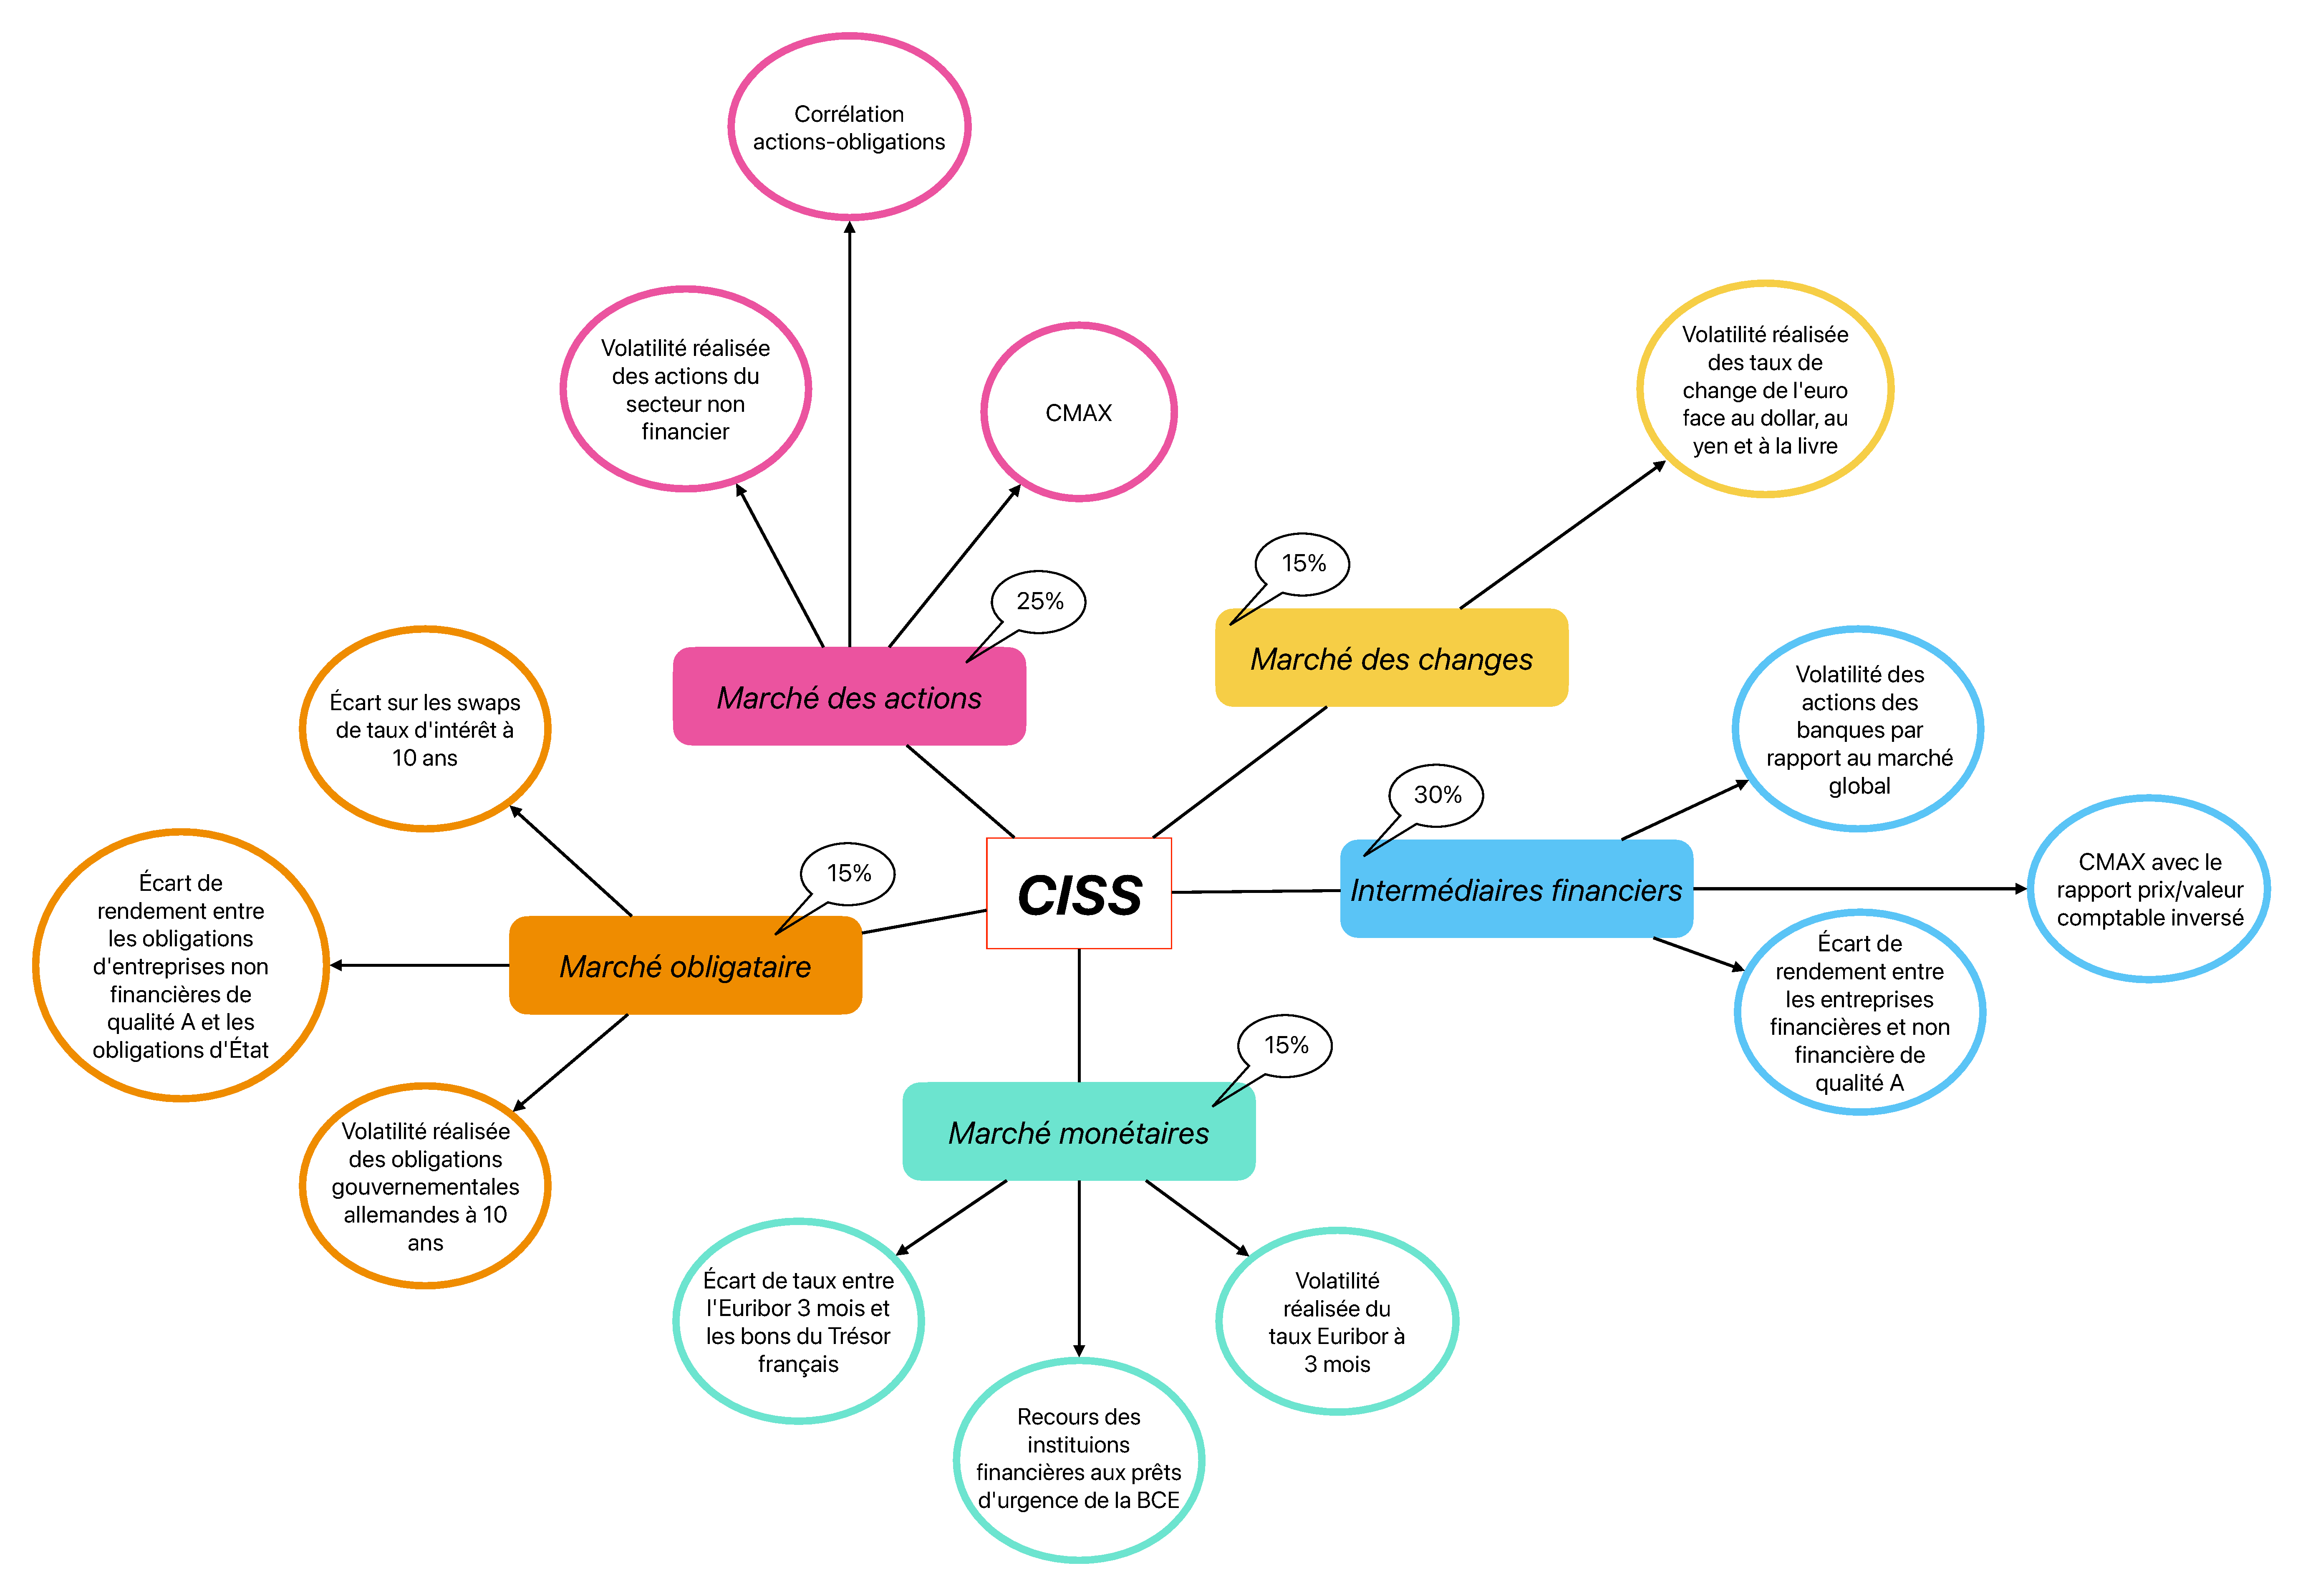
\includegraphics[width=1\linewidth]{figures/décomposition du CISS.pdf}
    \caption{Décomposition du CISS.}
    \label{fig:decomposition_ciss}
\end{sidewaysfigure}

\newpage

\section{Modélisation non-linéaire des sous indicateurs de stress systémique}\label{appendix:resultats}
\setcounter{table}{0}
\setcounter{figure}{0}

\begin{table}[H]
    \centering
    \caption{Test ARCH Forex.}
    \sffamily
    \begin{tabular}{lrrrr}
\toprule
\multicolumn{2}{l}{Heteroskedasticity Test: ARCH}&\multicolumn{1}{c}{}&\multicolumn{1}{c}{}&\multicolumn{1}{c}{}\\
[4.5pt] \hline \\ [-4.5pt]
\multicolumn{1}{l}{F-statistic}&\multicolumn{1}{r}{$267.4001$}&\multicolumn{2}{l}{Prob. F(1,225)}&\multicolumn{1}{r}{$0.0000$}\\
\multicolumn{1}{l}{Obs*R-squared}&\multicolumn{1}{r}{$123.2734$}&\multicolumn{2}{l}{Prob. Chi-Square(1)}&\multicolumn{1}{r}{$0.0000$}\\
[4.5pt] \bottomrule \\ [-4.5pt]
\end{tabular}

    \label{tab:arch_test_forex}
\end{table}

\begin{table}[H]
    \centering
    \caption{Test ARCH Equity.}
    \sffamily
    \begin{tabular}{lrrrr}
\toprule
\multicolumn{2}{l}{Heteroskedasticity Test: ARCH}&\multicolumn{1}{c}{}&\multicolumn{1}{c}{}&\multicolumn{1}{c}{}\\
[4.5pt] \hline \\ [-4.5pt]
\multicolumn{1}{l}{F-statistic}&\multicolumn{1}{r}{$209.9164$}&\multicolumn{2}{l}{Prob. F(1,225)}&\multicolumn{1}{r}{$0.0000$}\\
\multicolumn{1}{l}{Obs*R-squared}&\multicolumn{1}{r}{$109.5636$}&\multicolumn{2}{l}{Prob. Chi-Square(1)}&\multicolumn{1}{r}{$0.0000$}\\
[4.5pt] \bottomrule \\ [-4.5pt]
\end{tabular}

    \label{tab:arch_test_equity}
\end{table}

\begin{table}[H]
    \centering
    \caption{Test ARCH Imm.}
    \sffamily
    \begin{tabular}{lrrrr}
\toprule
\multicolumn{2}{l}{Heteroskedasticity Test: ARCH}&\multicolumn{1}{c}{}&\multicolumn{1}{c}{}&\multicolumn{1}{c}{}\\
[4.5pt] \hline \\ [-4.5pt]
\multicolumn{1}{l}{F-statistic}&\multicolumn{1}{r}{$484.0074$}&\multicolumn{2}{l}{Prob. F(1,225)}&\multicolumn{1}{r}{$0.0000$}\\
\multicolumn{1}{l}{Obs*R-squared}&\multicolumn{1}{r}{$154.9627$}&\multicolumn{2}{l}{Prob. Chi-Square(1)}&\multicolumn{1}{r}{$0.0000$}\\
[4.5pt] \bottomrule \\ 
\end{tabular}

    \label{tab:arch_test_imm}
\end{table}

\begin{figure}[H]
    \centering
    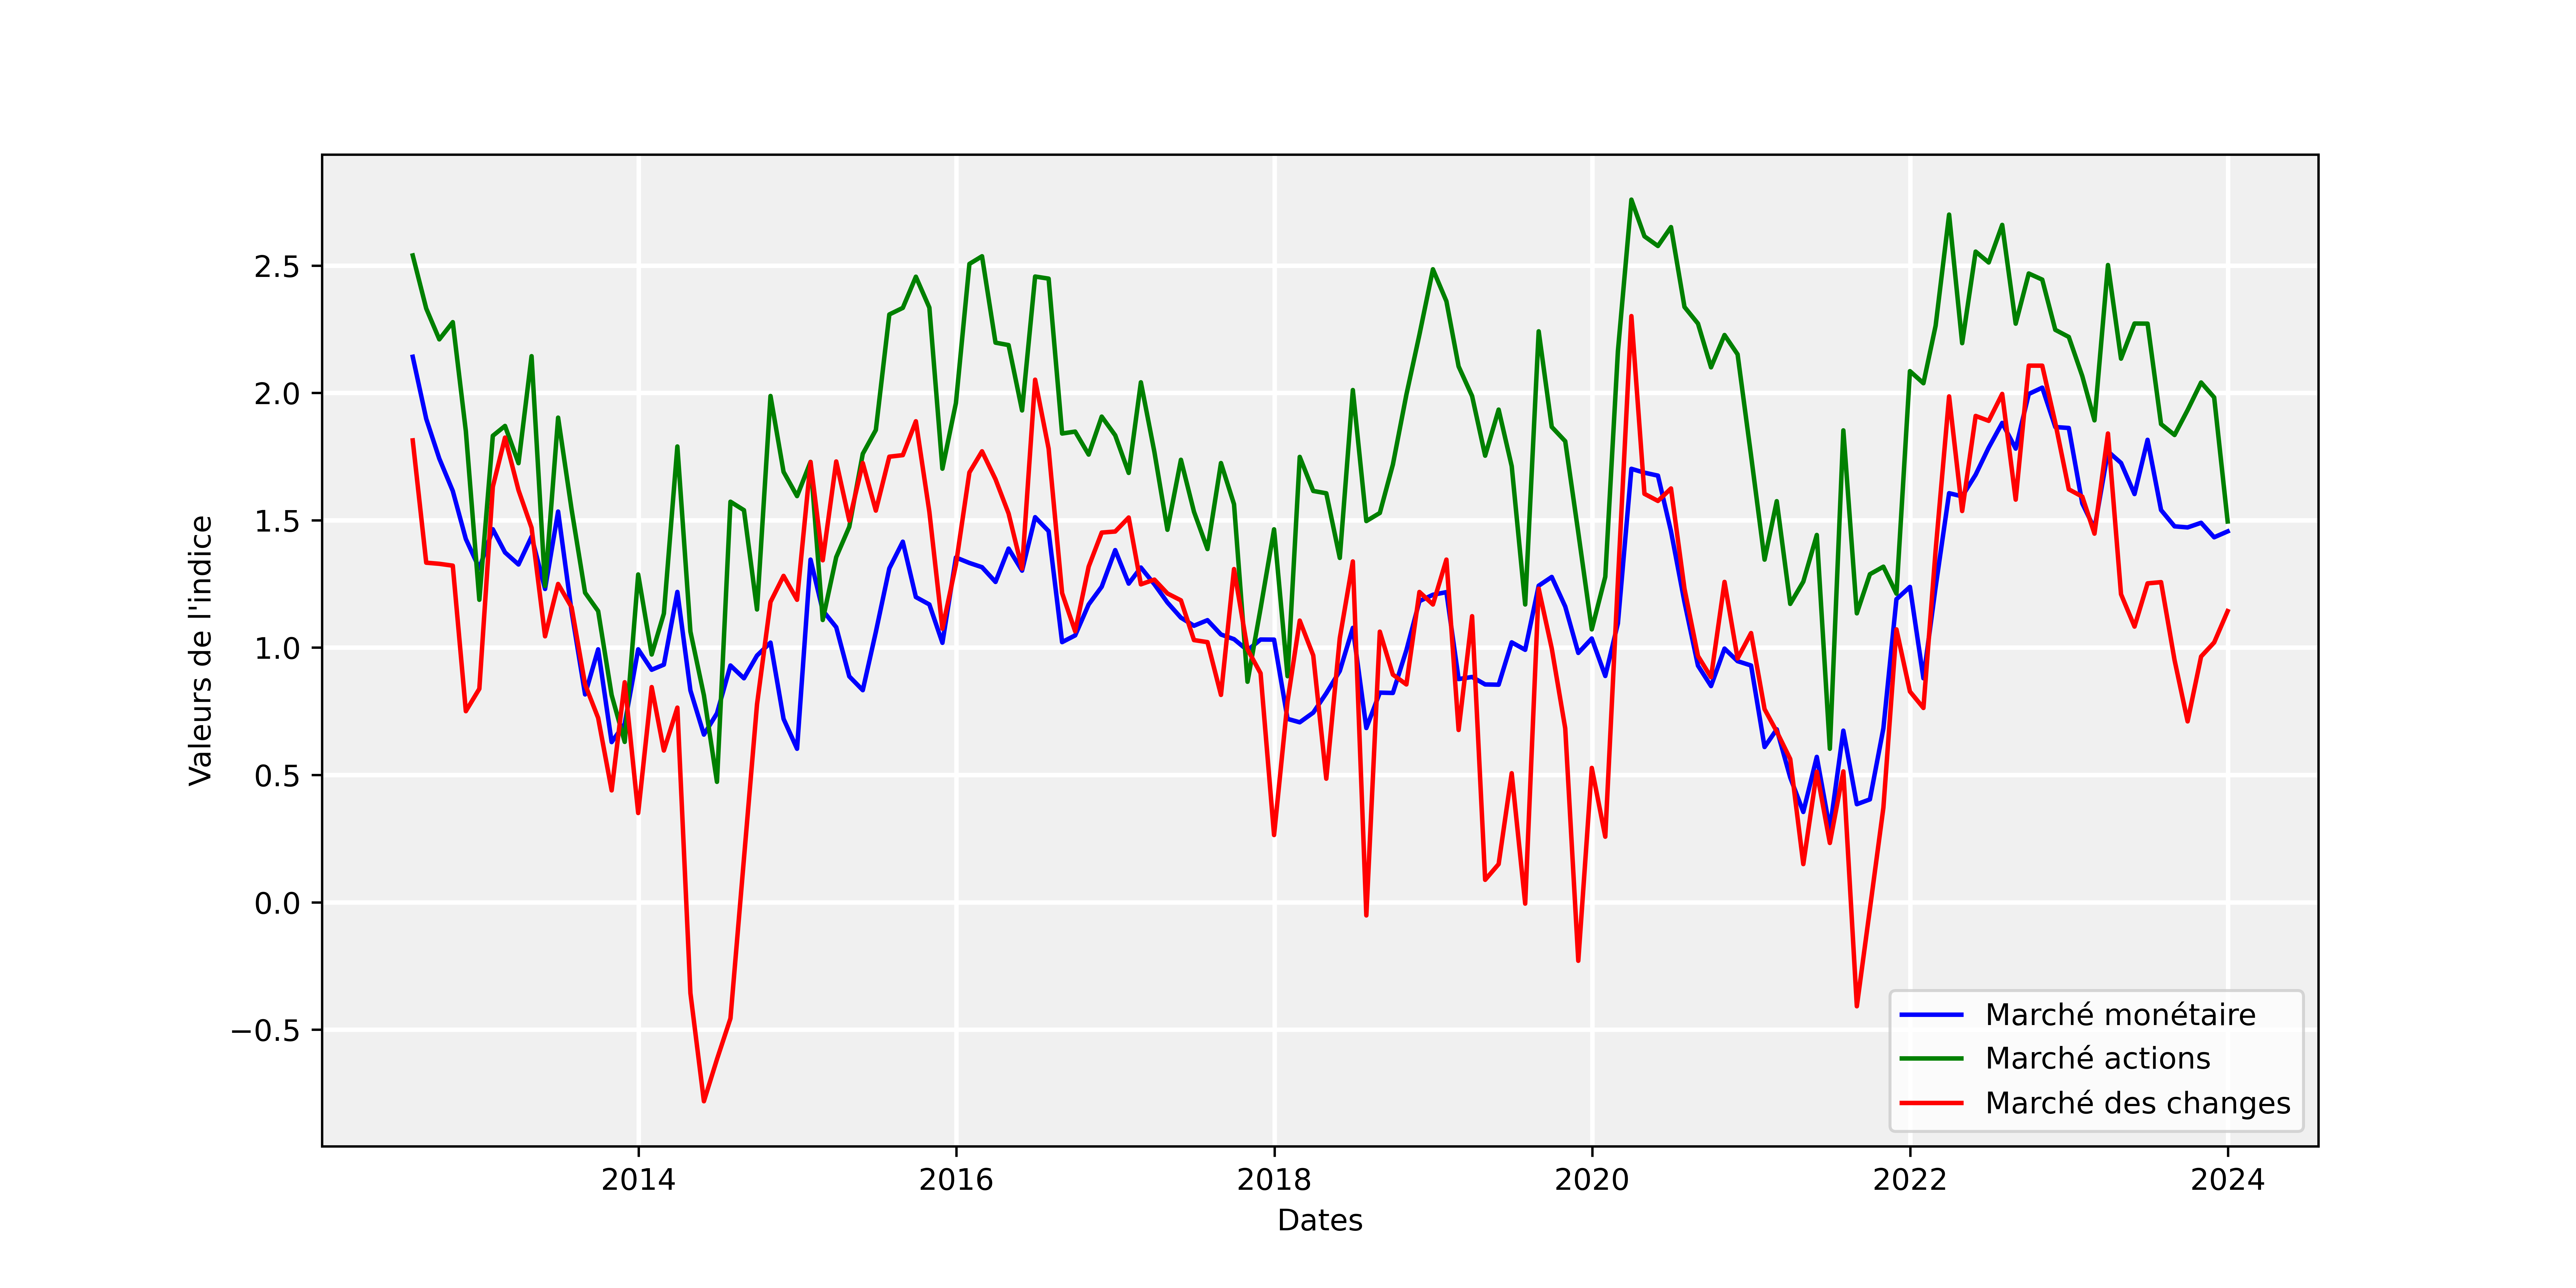
\includegraphics[width=1\linewidth]{annexes/sous_indicateurs_stress_log.png}
    \caption{Sous-indicateurs de stress en logarithme entre janvier 2005 et décembre 2024.}
    \label{fig:graphindicateurslog}
\end{figure}

\begin{figure}[H]
    \centering
    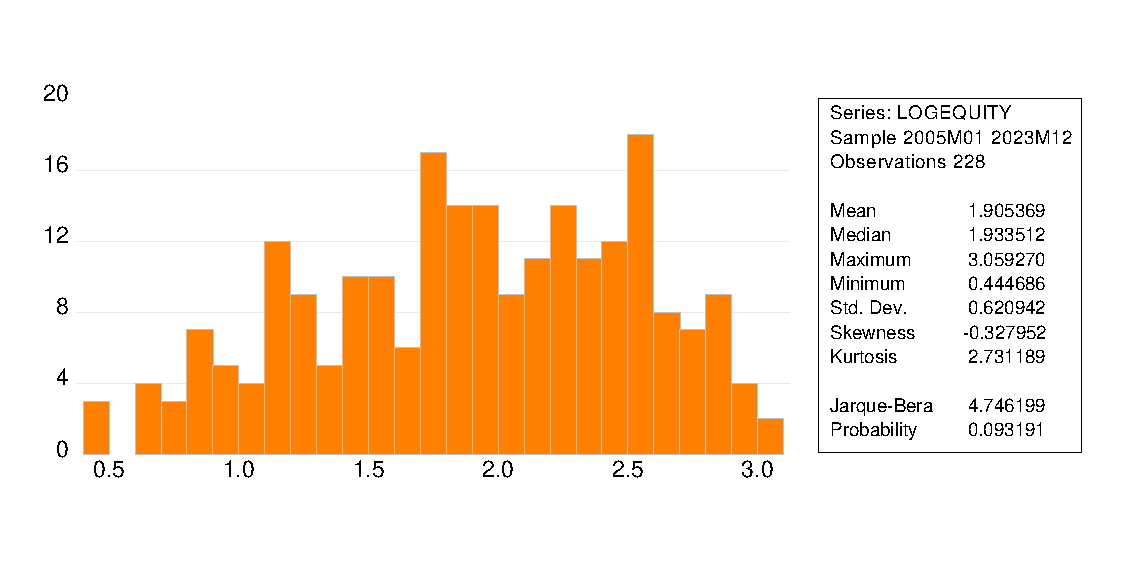
\includegraphics[width=1\linewidth]{annexes/jb_logequity.pdf}
    \caption{Test de normalité sur la série logequity.}
    \label{fig:normalitelogequity}
\end{figure}

\begin{figure}[H]
    \centering
    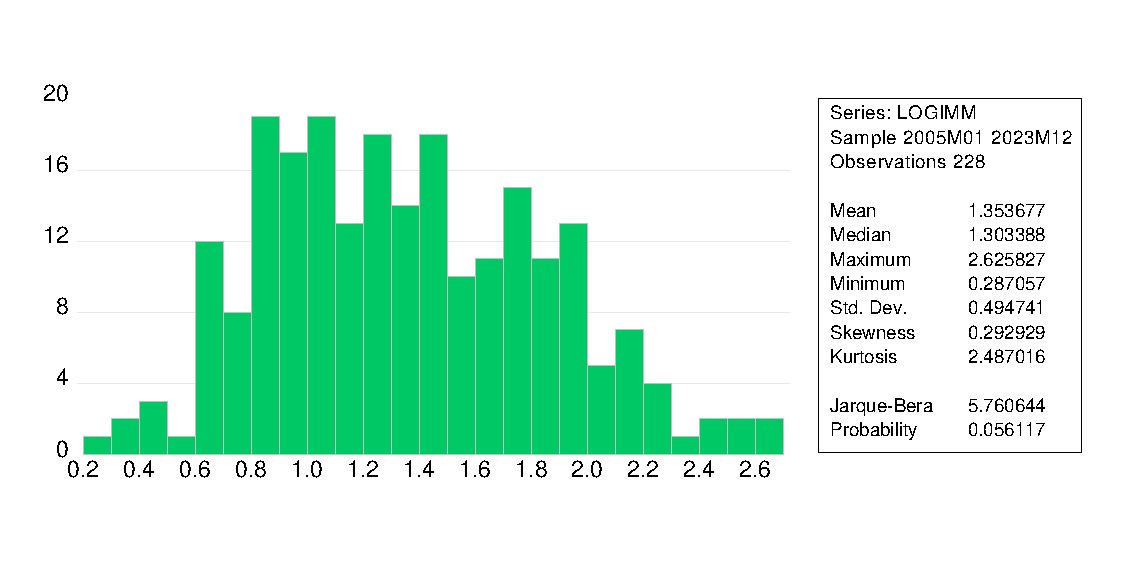
\includegraphics[width=1\linewidth]{annexes/jb_logimm.pdf}
    \caption{Test de normalité sur la série logimm.}
    \label{fig:normalitelogimm}
\end{figure}

\begin{figure}[H]
    \centering
    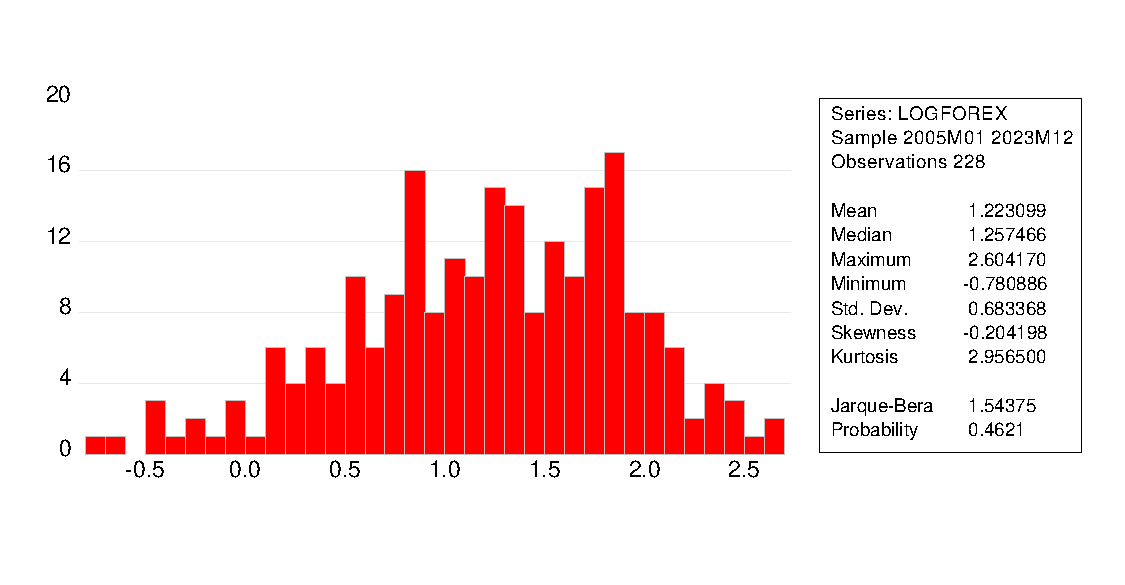
\includegraphics[width=1\linewidth]{annexes/jb_logforex.pdf}
    \caption{Test de normalité sur la série logforex.}
    \label{fig:normalitelogforex}
\end{figure}

\subsection{Détection de la saisonnalité et de la tendance}

\subsubsection*{Tests de Fischer}\label{appendix:fischer_test}

\begin{table}[H]
    \centering
    \caption[test]{Analyse de la variance}
    \sffamily 
    \resizebox{\textwidth}{!}{\begin{tabular}{lccl}
        \toprule
        Somme des carrés & Degré de liberté & Désignation & Variance\\
        \midrule
        $S_{p} = N \sum\limits_{j}(x_{\cdot j}- x_{\cdot \cdot})^2$ & $p-1$ & Variance Période & $V_{p} = \frac{S_{p}}{p-1}$ \\
        $S_{A} = P \sum\limits_{i}(x_{i \cdot}- x_{\cdot \cdot})^2$ & $N-1$ & Variance Année & $V_{A} = \frac{S_{A}}{N-1}$ \\
        $S_{R} = \sum_{i} \sum\limits_{j}(x_{ij}-x_{i\cdot}-x_{\cdot j} + x_{\cdot \cdot})^2$ & $(p-1)(N-1)$ & Variance Résidu & $V_{R} = \frac{S_{R}}{(p-1)(N-1)}$ \\
        $S_{T} $ & $N\times p-1$ & Variance Totale & $V_{T} = \frac{S_{T}}{N\times p-1}$ \\
        \bottomrule
\end{tabular}}
    \label{tab:anova}
\end{table}

\begin{table}[H]
    \centering
    \caption{Analyse de la variance du marché actions (equity)}
    \sffamily
    \begin{tabular}{rrrr}
\toprule
    \textbf{Somme des carrés} & \textbf{Degrés de liberté} & \textbf{Désignation} & \textbf{Variance} \\
\midrule
   109,92 & 11 & Variance période &  9,99 \\ 
   5643,99 & 17  & Variance année & 332,00  \\ 
   1519,97 & 187 & Variance résidus &  8,13 \\ 
\bottomrule 
\end{tabular}
    \label{tab:anova_equity}
\end{table}

\begin{table}[H]
    \centering
    \caption{Analyse de la variance du marché des changes (forex)}
    \sffamily
    \begin{tabular}{rrrr}
\toprule
    \textbf{Somme des carrés} & \textbf{Degrés de liberté} & \textbf{Désignation} & \textbf{Variance} \\
\midrule
    36,16 & 11 & Variance période &  3,29 \\ 
    1747,29 & 17  & Variance année & 102,78  \\ 
   513,47  & 187 & Variance résidus &  2,75 \\ 
\bottomrule 
\end{tabular}
    \label{tab:anova_forex}
\end{table}

\begin{table}[H]
    \centering
    \caption{Analyse de la variance du marché interbancaire (imm)}
    \sffamily
    \begin{tabular}{rrrr}
\toprule
    \textbf{Somme des carrés} & \textbf{Degrés de liberté} & \textbf{Désignation} & \textbf{Variance} \\
\midrule
    18,77 & 11 & Variance période &  1,71 \\ 
    1633,77 & 17  & Variance année & 96,10  \\ 
   395,93  & 187 & Variance résidus &  2,12 \\ 
\bottomrule 
\end{tabular}
    \label{tab:anova_imm}
\end{table}

\subsubsection*{Buys-Ballot}

\begin{table}[H]
    \centering
    \caption{Tableau de Buys-Ballot pour le marché des changes (forex)}
    \sffamily
    \resizebox{1\textwidth}{!}{\renewcommand{\arraystretch}{1.3} % pour augmenter l'espacement vertical
\begin{tabular}{|l|l|l|l|l|l|l|l|l|l|l|l|l|l|l|}
    \hline
    \textbf{années} & \textbf{janvier} & \textbf{février} & \textbf{mars} & \textbf{avril} & \textbf{mai} & \textbf{juin} & \textbf{juillet} & \textbf{août} & \textbf{septembre} & \textbf{octobre} & \textbf{novembre} & \textbf{décembre} & \textbf{$\bm{x}_{i.}$} & \textbf{$\bm{\sigma}_{i.}$} \\ \hline
    \textbf{2005} & 2,00 & 1,36 & 1,48 & 1,78 & 1,68 & 3,78 & 2,47 & 1,48 & 1,32 & 2,33 & 2,30 & 1,72 & 1,98 & 0,66 \\ \hline
    \textbf{2006} & 2,37 & 1,81 & 2,39 & 2,36 & 3,17 & 2,03 & 2,01 & 1,19 & 1,84 & 0,81 & 1,13 & 0,88 & 1,83 & 0,68 \\ \hline
    \textbf{2007} & 1,58 & 1,50 & 3,19 & 1,20 & 0,64 & 1,42 & 2,26 & 5,59 & 4,29 & 3,45 & 6,29 & 5,84 & 3,10 & 1,90 \\ \hline
    \textbf{2008} & 7,83 & 4,79 & 8,40 & 7,40 & 4,72 & 5,95 & 4,24 & 7,14 & 9,94 & 13,52 & 13,48 & 10,99 & 8,20 & 3,07 \\ \hline
    \textbf{2009} & 12,24 & 11,75 & 11,54 & 10,75 & 9,92 & 10,11 & 7,74 & 6,45 & 4,88 & 6,50 & 6,41 & 4,96 & 8,61 & 2,62 \\ \hline
    \textbf{2010} & 6,00 & 6,53 & 5,52 & 6,63 & 11,83 & 7,19 & 7,02 & 6,26 & 7,88 & 6,54 & 6,95 & 5,33 & 6,97 & 1,61 \\ \hline
    \textbf{2011} & 6,66 & 4,45 & 5,60 & 5,97 & 6,77 & 6,56 & 7,48 & 8,42 & 8,64 & 8,86 & 7,63 & 4,02 & 6,76 & 1,50 \\ \hline
    \textbf{2012} & 7,78 & 5,68 & 4,54 & 3,98 & 4,99 & 6,57 & 6,13 & 3,79 & 3,78 & 3,75 & 2,12 & 2,31 & 4,62 & 1,62 \\ \hline
    \textbf{2013} & 5,11 & 6,20 & 5,04 & 4,35 & 2,84 & 3,49 & 3,19 & 2,35 & 2,06 & 1,55 & 2,37 & 1,42 & 3,33 & 1,47 \\ \hline
    \textbf{2014} & 2,33 & 1,82 & 2,15 & 0,70 & 0,46 & 0,54 & 0,63 & 1,19 & 2,18 & 3,25 & 3,60 & 3,28 & 1,84 & 1,10 \\ \hline
    \textbf{2015} & 5,63 & 3,83 & 5,65 & 4,48 & 5,61 & 4,66 & 5,75 & 5,79 & 6,61 & 4,63 & 2,93 & 3,76 & 4,94 & 1,03 \\ \hline
    \textbf{2016} & 5,41 & 5,88 & 5,26 & 4,60 & 3,71 & 7,78 & 5,94 & 3,37 & 2,90 & 3,74 & 4,27 & 4,29 & 4,76 & 1,31 \\ \hline
    \textbf{2017} & 4,53 & 3,49 & 3,55 & 3,36 & 3,27 & 2,80 & 2,78 & 2,26 & 3,70 & 2,70 & 2,46 & 1,30 & 3,02 & 0,79 \\ \hline
    \textbf{2018} & 2,20 & 3,02 & 2,64 & 1,63 & 2,82 & 3,81 & 0,95 & 2,89 & 2,45 & 2,35 & 3,38 & 3,22 & 2,61 & 0,75 \\ \hline
    \textbf{2019} & 3,84 & 1,97 & 3,08 & 1,09 & 1,16 & 1,66 & 1,00 & 3,43 & 2,71 & 1,98 & 0,80 & 1,70 & 2,03 & 0,97 \\ \hline
    \textbf{2020} & 1,29 & 3,53 & 9,99 & 4,97 & 4,84 & 5,08 & 3,42 & 2,63 & 2,42 & 3,52 & 2,61 & 2,88 & 3,93 & 2,13 \\ \hline
    \textbf{2021} & 2,14 & 1,96 & 1,76 & 1,16 & 1,67 & 1,26 & 1,67 & 0,67 & 0,97 & 1,45 & 2,92 & 2,29 & 1,66 & 0,59 \\ \hline
    \textbf{2022} & 2,15 & 3,98 & 7,29 & 4,65 & 6,75 & 6,62 & 7,36 & 4,86 & 8,22 & 8,22 & 6,57 & 5,06 & 5,98 & 1,77 \\ \hline
    \textbf{2023} & 4,92 & 4,25 & 6,30 & 3,35 & 2,95 & 3,50 & 3,52 & 2,59 & 2,04 & 2,63 & 2,77 & 3,14 & 3,50 & 1,12 \\ \hline
    \textbf{$\bm{x}_{.j}$} & 4,53 & 4,09 & 5,02 & 3,92 & 4,20 & 4,46 & 3,98 & 3,81 & 4,15 & 4,30 & 4,26 & 3,60 & $\bm{x}_{..}$ & $\bm{\sigma}_{..}$ \\ \hline
    \textbf{$\bm{\sigma}_{.j}$} & 2,74 & 2,42 & 2,72 & 2,50 & 2,93 & 2,52 & 2,35 & 2,19 & 2,68 & 3,08 & 2,94 & 2,25 & 3,46 & 2,88 \\ \hline
\end{tabular}
}
    \label{tab:bb_forex}
\end{table}

\begin{table}[H]
    \centering
    \caption{Tableau de Buys-Ballot pour le marché interbancaire (imm)}
    \sffamily
    \resizebox{1\textwidth}{!}{\renewcommand{\arraystretch}{1.3} % pour augmenter l'espacement vertical
\begin{tabular}{|l|l|l|l|l|l|l|l|l|l|l|l|l|l|l|}
    \hline
    \textbf{années} & \textbf{janvier} & \textbf{février} & \textbf{mars} & \textbf{avril} & \textbf{mai} & \textbf{juin} & \textbf{juillet} & \textbf{août} & \textbf{septembre} & \textbf{octobre} & \textbf{novembre} & \textbf{décembre} & \textbf{$\bm{x}_{i.}$} & \textbf{$\bm{\sigma}_{i.}$} \\ \hline
    \textbf{2005} & 1,89 & 1,94 & 1,87 & 2,44 & 2,07 & 2,67 & 2,07 & 1,50 & 1,89 & 2,94 & 3,47 & 2,42 & 2,26 & 0,53 \\ \hline
    \textbf{2006} & 2,98 & 2,85 & 3,09 & 3,63 & 4,34 & 4,25 & 4,48 & 3,69 & 3,87 & 3,39 & 2,82 & 2,72 & 3,51 & 0,60 \\ \hline
    \textbf{2007} & 2,44 & 2,38 & 3,52 & 4,53 & 3,54 & 3,35 & 4,27 & 7,74 & 6,80 & 5,82 & 6,82 & 7,99 & 4,93 & 1,93 \\ \hline
    \textbf{2008} & 8,52 & 6,64 & 9,19 & 6,49 & 5,12 & 6,74 & 5,20 & 4,76 & 8,41 & 13,82 & 13,74 & 12,54 & 8,43 & 3,15 \\ \hline
    \textbf{2009} & 12,53 & 11,53 & 11,46 & 9,07 & 7,27 & 9,56 & 7,85 & 6,26 & 5,57 & 5,68 & 5,63 & 4,74 & 8,10 & 2,57 \\ \hline
    \textbf{2010} & 5,08 & 5,21 & 4,61 & 4,42 & 6,96 & 6,49 & 6,84 & 5,59 & 6,41 & 6,85 & 6,15 & 5,51 & 5,84 & 0,86 \\ \hline
    \textbf{2011} & 4,29 & 5,48 & 6,78 & 5,97 & 4,47 & 5,47 & 5,63 & 7,88 & 7,18 & 9,01 & 9,73 & 8,86 & 6,73 & 1,74 \\ \hline
    \textbf{2012} & 10,22 & 8,34 & 8,38 & 7,13 & 7,03 & 6,88 & 8,52 & 6,67 & 5,71 & 5,03 & 4,16 & 3,71 & 6,81 & 1,84 \\ \hline
    \textbf{2013} & 4,33 & 3,95 & 3,77 & 4,20 & 3,42 & 4,64 & 3,13 & 2,26 & 2,70 & 1,88 & 2,02 & 2,70 & 3,25 & 0,90 \\ \hline
    \textbf{2014} & 2,49 & 2,54 & 3,38 & 2,30 & 1,93 & 2,10 & 2,53 & 2,41 & 2,64 & 2,77 & 2,06 & 1,83 & 2,42 & 0,41 \\ \hline
    \textbf{2015} & 3,84 & 3,15 & 2,95 & 2,43 & 2,30 & 2,89 & 3,71 & 4,12 & 3,32 & 3,22 & 2,77 & 3,87 & 3,21 & 0,56 \\ \hline
    \textbf{2016} & 3,79 & 3,73 & 3,52 & 4,01 & 3,68 & 4,54 & 4,30 & 2,78 & 2,85 & 3,22 & 3,45 & 3,99 & 3,65 & 0,51 \\ \hline
    \textbf{2017} & 3,50 & 3,72 & 3,49 & 3,25 & 3,06 & 2,96 & 3,03 & 2,86 & 2,81 & 2,69 & 2,81 & 2,81 & 3,08 & 0,32 \\ \hline
    \textbf{2018} & 2,06 & 2,03 & 2,11 & 2,27 & 2,48 & 2,94 & 1,98 & 2,28 & 2,28 & 2,69 & 3,26 & 3,35 & 2,48 & 0,46 \\ \hline
    \textbf{2019} & 3,38 & 2,40 & 2,42 & 2,35 & 2,35 & 2,78 & 2,70 & 3,47 & 3,59 & 3,19 & 2,66 & 2,82 & 2,84 & 0,43 \\ \hline
    \textbf{2020} & 2,43 & 2,99 & 5,49 & 5,40 & 5,34 & 4,29 & 3,25 & 2,53 & 2,34 & 2,71 & 2,58 & 2,53 & 3,49 & 1,22 \\ \hline
    \textbf{2021} & 1,84 & 1,97 & 1,63 & 1,43 & 1,77 & 1,33 & 1,96 & 1,47 & 1,50 & 1,98 & 3,29 & 3,45 & 1,97 & 0,66 \\ \hline
    \textbf{2022} & 2,41 & 3,45 & 4,98 & 4,92 & 5,36 & 5,96 & 6,57 & 5,94 & 7,36 & 7,54 & 6,46 & 6,44 & 5,62 & 1,45 \\ \hline
    \textbf{2023} & 4,79 & 4,34 & 5,87 & 5,61 & 4,97 & 6,15 & 4,67 & 4,38 & 4,36 & 4,44 & 4,19 & 4,29 & 4,84 & 0,65 \\ \hline
    \textbf{$\bm{x}_{.j}$} & 4,36 & 4,14 & 4,66 & 4,31 & 4,08 & 4,53 & 4,35 & 4,14 & 4,29 & 4,68 & 4,64 & 4,56 & $\bm{x}_{..}$ & $\bm{\sigma}_{..}$ \\ \hline
    \textbf{$\bm{\sigma}_{.j}$} & 2,86 & 2,39 & 2,59 & 1,93 & 1,73 & 2,01 & 1,93 & 1,98 & 2,07 & 2,90 & 2,89 & 2,63 & 3,63 & 2,72 \\ \hline
\end{tabular}
}
    \label{tab:bb_imm}
\end{table}

\begin{table}[H]
    \centering
    \caption{Tableau de Buys-Ballot pour le marché actions (equity)}
    \sffamily
    \resizebox{1\textwidth}{!}{\renewcommand{\arraystretch}{1.3} % pour augmenter l'espacement vertical
\begin{tabular}{|l|l|l|l|l|l|l|l|l|l|l|l|l|l|l|}
    \hline
    \textbf{années} & \textbf{janvier} & \textbf{février} & \textbf{mars} & \textbf{avril} & \textbf{mai} & \textbf{juin} & \textbf{juillet} & \textbf{août} & \textbf{septembre} & \textbf{octobre} & \textbf{novembre} & \textbf{décembre}& \textbf{$\bm{x}_{i.}$} & \textbf{$\bm{\sigma}_{i.}$} \\ \hline
    \textbf{2005} & \hspace{3pt}1,56 & 2,16 & 2,01 & 3,62 & 3,41 & 2,42 & 2,52 & 2,26 & 2,18 & 4,77 & 3,21 & 1,57 & 2,64 & 0,90 \\ \hline
    \textbf{2006} & 2,96 & 2,71 & 2,72 & 2,79 & 6,09 & 7,74 & 7,05 & 4,22 & 4,10 & 2,41 & 3,08 & 3,18 & 4,09 & 1,77 \\ \hline
    \textbf{2007} & 2,15 & 1,86 & 7,52 & 4,34 & 2,61 & 4,65 & 7,32 & 14,35 & 12,33 & 8,02 & 12,02 & 10,43 & 7,30 & 4,10 \\ \hline
    \textbf{2008} & 15,72 & 16,02 & 17,89 & 15,30 & 11,46 & 14,48 & 12,90 & 13,27 & 18,81 & 21,31 & 20,16 & 16,56 & 16,16 & 2,85 \\ \hline
    \textbf{2009} & 16,09 & 17,10 & 19,53 & 16,86 & 14,67 & 17,24 & 16,67 & 14,14 & 10,87 & 13,77 & 12,24 & 11,07 & 15,02 & 2,58 \\ \hline
    \textbf{2010} & 11,49 & 12,52 & 9,84 & 10,92 & 18,48 & 15,15 & 12,80 & 12,17 & 10,29 & 6,77 & 5,93 & 5,78 & 11,01 & 3,57 \\ \hline
    \textbf{2011} & 5,22 & 4,97 & 8,60 & 7,24 & 6,01 & 10,42 & 12,80 & 16,90 & 18,24 & 17,56 & 16,75 & 12,27 & 11,42 & 4,84 \\ \hline
    \textbf{2012} & 11,45 & 8,65 & 9,35 & 12,58 & 13,40 & 12,70 & 12,68 & 10,29 & 9,12 & 9,76 & 6,36 & 3,28 & 9,97 & 2,83 \\ \hline
    \textbf{2013} & 6,24 & 6,49 & 5,61 & 8,54 & 3,46 & 6,71 & 4,68 & 3,37 & 3,14 & 2,26 & 1,88 & 3,62 & 4,67 & 1,96 \\ \hline
    \textbf{2014} & 2,65 & 3,11 & 5,99 & 2,90 & 2,25 & 1,61 & 4,82 & 4,66 & 3,16 & 7,30 & 5,42 & 4,93 & 4,07 & 1,64 \\ \hline
    \textbf{2015} & 5,64 & 3,03 & 3,88 & 4,37 & 5,82 & 6,39 & 10,05 & 10,32 & 11,66 & 10,33 & 5,49 & 7,10 & 7,01 & 2,76 \\ \hline
    \textbf{2016} & 12,26 & 12,64 & 9,00 & 8,92 & 6,90 & 11,67 & 11,57 & 6,30 & 6,35 & 5,80 & 6,73 & 6,26 & 8,70 & 2,55 \\ \hline
    \textbf{2017} & 5,40 & 7,70 & 5,86 & 4,32 & 5,68 & 4,63 & 4,00 & 5,61 & 4,77 & 2,38 & 3,17 & 4,33 & 4,82 & 1,32 \\ \hline
    \textbf{2018} & 2,43 & 5,75 & 5,03 & 4,98 & 3,87 & 7,47 & 4,47 & 4,61 & 5,58 & 7,34 & 9,29 & 12,01 & 6,07 & 2,49 \\ \hline
    \textbf{2019} & 10,59 & 8,20 & 7,30 & 5,78 & 6,92 & 5,54 & 3,22 & 9,41 & 6,47 & 6,11 & 4,27 & 2,92 & 6,39 & 2,22 \\ \hline
    \textbf{2020} & 3,59 & 8,70 & 15,78 & 13,66 & 13,16 & 14,17 & 10,35 & 9,70 & 8,17 & 9,27 & 8,60 & 5,77 & 10,08 & 3,43 \\ \hline
    \textbf{2021} & 3,84 & 4,83 & 3,23 & 3,52 & 4,23 & 1,83 & 6,38 & 3,11 & 3,63 & 3,74 & 3,36 & 8,05 & 4,14 & 1,57 \\ \hline
    \textbf{2022} & 7,68 & 9,62 & 14,88 & 8,98 & 12,87 & 12,33 & 14,29 & 9,70 & 11,81 & 11,53 & 9,47 & 9,20 & 11,03 & 2,17 \\ \hline
    \textbf{2023} & 7,89 & 6,64 & 12,21 & 8,45 & 9,70 & 9,70 & 6,54 & 6,26 & 6,91 & 7,70 & 7,26 & 4,46 & 7,81 & 1,93 \\ \hline
    \textbf{$\bm{x}_{.j}$} & 7,10 & 7,51 & 8,75 & 7,79 & 7,95 & 8,78 & 8,69 & 8,46 & 8,29 & 8,32 & 7,61 & 6,99 & $\bm{x}_{..}$ & $\bm{\sigma}_{..}$ \\ \hline
    \textbf{$\bm{\sigma}_{.j}$} & 4,47 & 4,38 & 5,02 & 4,24 & 4,61 & 4,65 & 4,16 & 4,25 & 4,70 & 4,91 & 4,73 & 3,88 & 6,62 & 5,13 \\ \hline
\end{tabular}
}
    \label{tab:bb_equity}
\end{table}

\subsection{Analyse de la stationnarité}

\subsubsection*{Analyse du corrélogramme}\label{appendix:correlo}

\begin{figure}[H]
    \centering
    \caption{Correlogramme du forex}
     \resizebox{0.6\textwidth}{!}{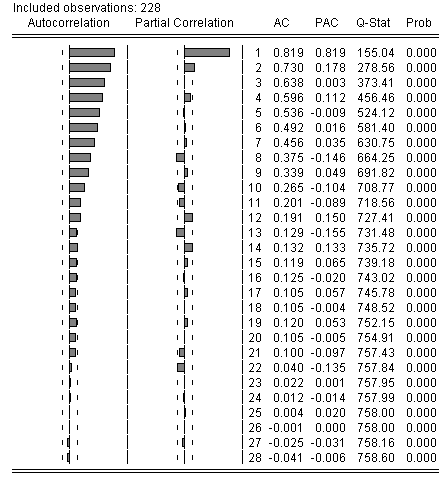
\includegraphics{annexes/correlo_logforex.png}}
    \label{tab:correlo_forex}
\end{figure}

\begin{figure}[H]
    \centering
    \caption{Correlogramme d'equity}
     \resizebox{0.6\textwidth}{!}{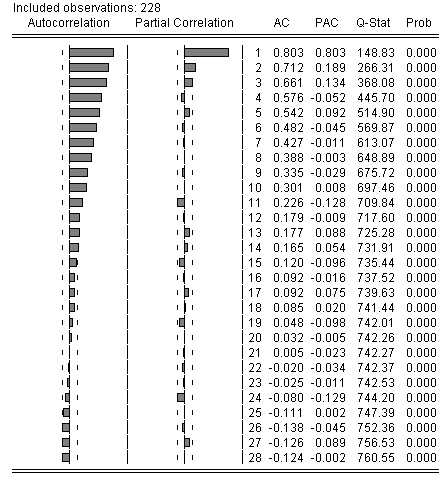
\includegraphics{annexes/correlo_logequity.png}}
    \label{tab:correlo_equity}
\end{figure}

\begin{figure}[H]
    \centering
    \caption{Correlogramme d'imm}
     \resizebox{0.6\textwidth}{!}{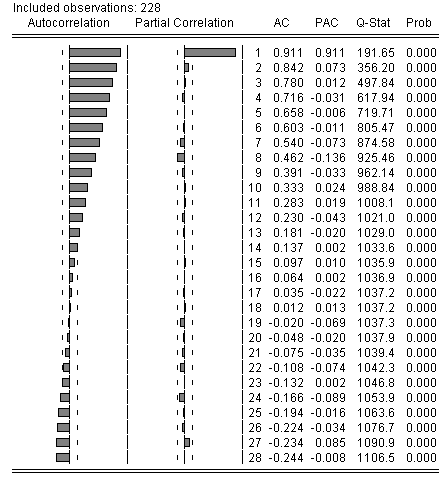
\includegraphics{annexes/correlo_logimm.png}}
    \label{tab:correlo_imm}
\end{figure}

\subsubsection*{Test de racine unitaire}

\begin{figure}[H]
    \centering
    \caption{Stratégie de Dickey-Fuller}
    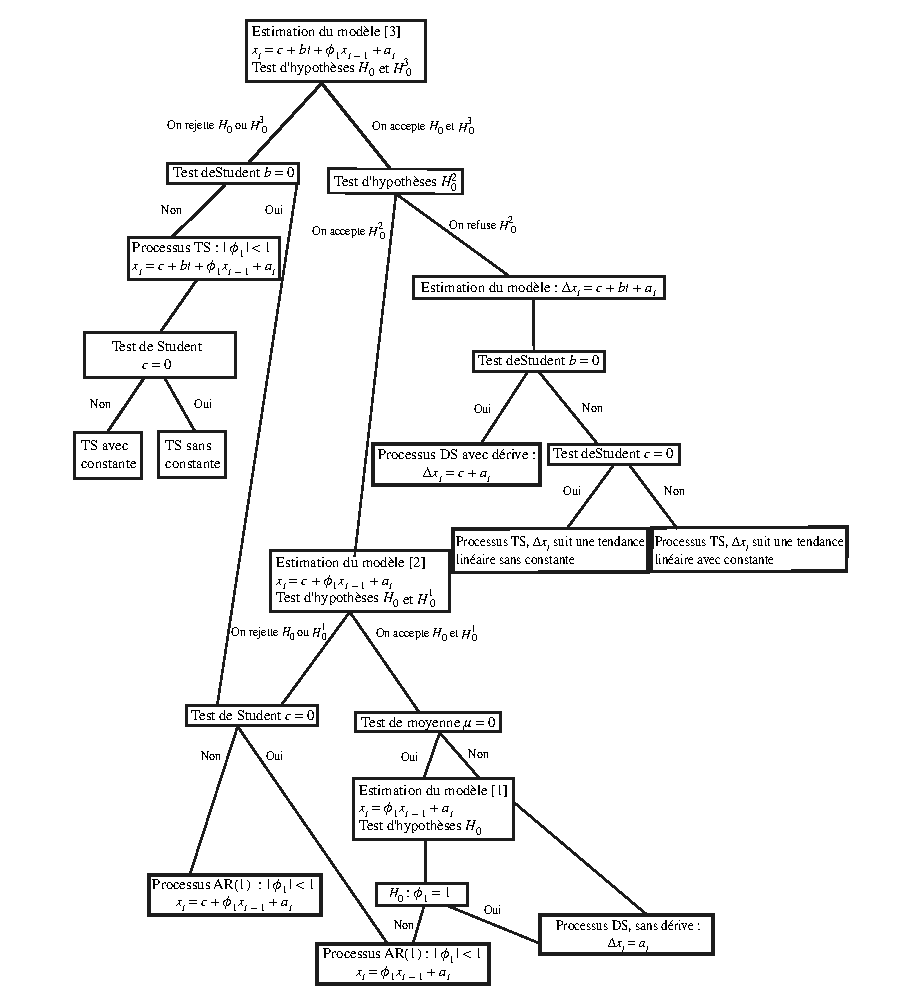
\includegraphics[scale=1.2]{annexes/df_test.pdf}
    \label{fig:strategie}
\end{figure}

\begin{figure}[H]
    \centering
    \caption{Distribution empirique de $\Phi_1$ pour $H_0^1$ (modèle 2).}
    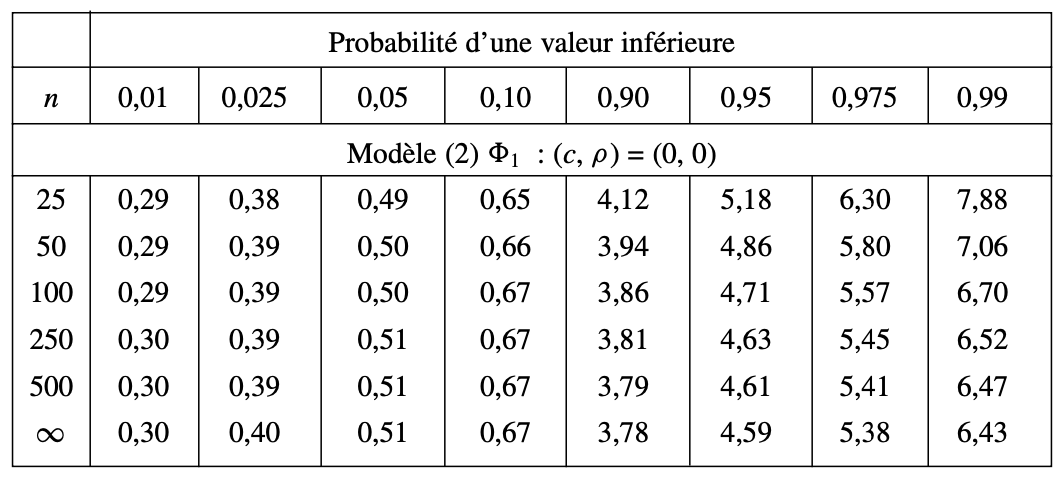
\includegraphics[scale=0.8]{annexes/dfvalues1.png}
    \label{fig:tabledf1}
\end{figure}

\begin{figure}[H]
    \centering
    \caption{Distribution empirique de $\Phi_2$ pour $H_0^2$ (modèle 3).}
    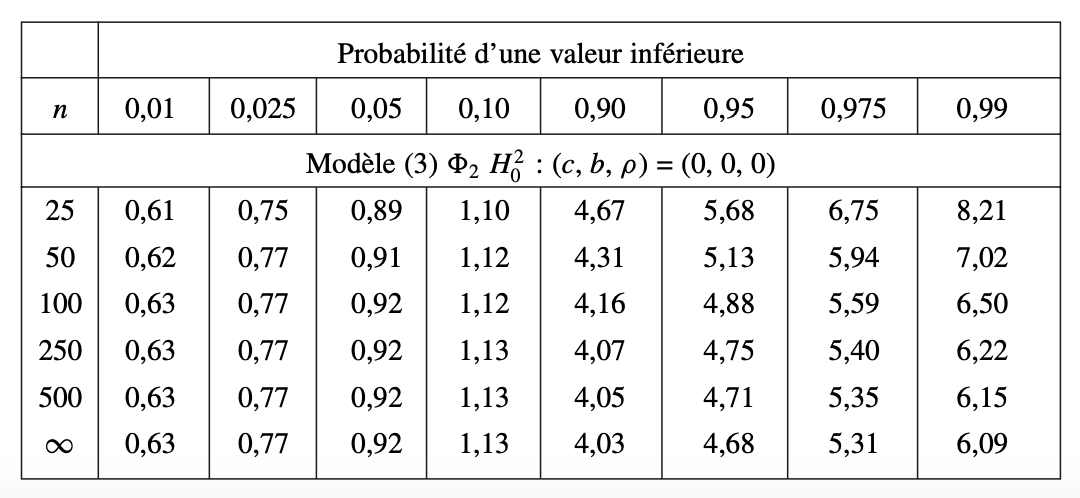
\includegraphics[scale=0.8]{annexes/dfvalues2.png}
    \label{fig:tabledf2}
\end{figure}

\begin{figure}[H]
    \centering
    \caption{Distribution empirique de $\Phi_3$ pour $H_0^3$ (modèle 3).}
    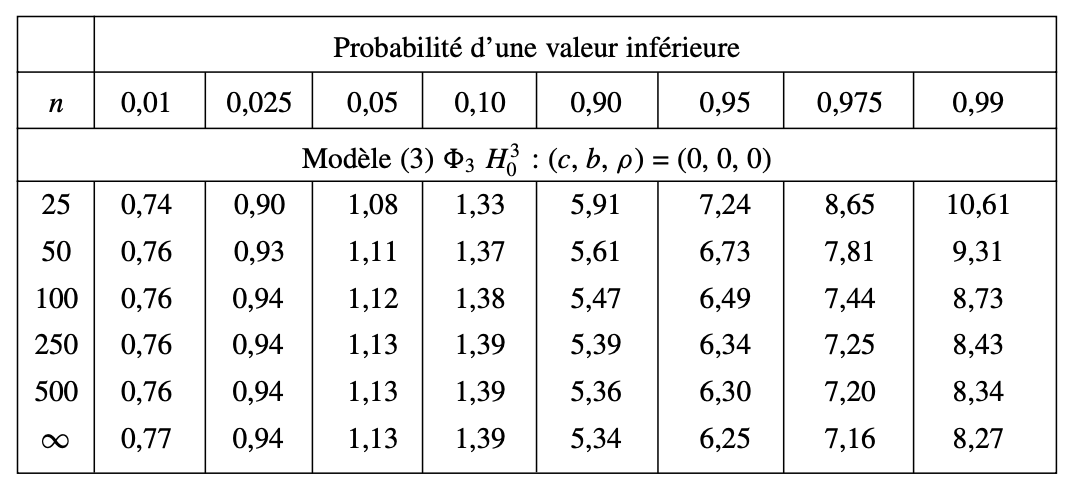
\includegraphics[scale=0.8]{annexes/dfvalues3.png}
    \label{fig:tabledf3}
\end{figure}

\begin{table}[H]
    \centering
    \caption{Estimation du modèle 3 du marché actions (equity).}
    \sffamily
    \resizebox{0.8\textwidth}{!}{\begin{tabular}{lrrrr}
\multicolumn{4}{l}{Null Hypothesis: LOGEQUITY has a unit root}&\multicolumn{1}{c}{}\\
\multicolumn{3}{l}{Exogenous: Constant, Linear Trend}&\multicolumn{1}{c}{}&\multicolumn{1}{c}{}\\
\multicolumn{5}{l}{Bandwidth: 1 (Newey-West automatic) using Bartlett kernel}\\
[4.5pt] \hline \\ [-4.5pt]
\multicolumn{1}{c}{}&\multicolumn{1}{c}{}&\multicolumn{1}{c}{}&\multicolumn{1}{c}{Adj. t-Stat}&\multicolumn{1}{c}{Prob.*}\\
[4.5pt] \hline \\ [-4.5pt]
\multicolumn{2}{l}{Phillips-Perron test statistic}&\multicolumn{1}{l}{}&\multicolumn{1}{c}{$-4.778553$}&\multicolumn{1}{c}{$0.0007$}\\
\multicolumn{1}{l}{Test critical values:}&\multicolumn{1}{c}{1\% level}&\multicolumn{1}{c}{}&\multicolumn{1}{c}{$-3.998997$}&\multicolumn{1}{c}{}\\
\multicolumn{1}{c}{}&\multicolumn{1}{c}{5\% level}&\multicolumn{1}{c}{}&\multicolumn{1}{c}{$-3.429745$}&\multicolumn{1}{c}{}\\
\multicolumn{1}{c}{}&\multicolumn{1}{c}{10\% level}&\multicolumn{1}{c}{}&\multicolumn{1}{c}{$-3.138397$}&\multicolumn{1}{c}{}\\
[4.5pt] \hline \\ [-4.5pt]
\multicolumn{2}{l}{Phillips-Perron Test Equation}&\multicolumn{1}{c}{}&\multicolumn{1}{c}{}&\multicolumn{1}{c}{}\\
\multicolumn{3}{l}{Dependent Variable: D(LOGEQUITY)}&\multicolumn{1}{c}{}&\multicolumn{1}{c}{}\\
\multicolumn{2}{l}{Method: Least Squares}&\multicolumn{1}{c}{}&\multicolumn{1}{c}{}&\multicolumn{1}{c}{}\\
\multicolumn{3}{l}{Sample (adjusted): 2005M02 2023M12}&\multicolumn{1}{c}{}&\multicolumn{1}{c}{}\\
\multicolumn{4}{l}{Included observations: 227 after adjustments}&\multicolumn{1}{c}{}\\
[4.5pt] \hline \\ [-4.5pt]
\multicolumn{1}{c}{Variable}&\multicolumn{1}{r}{Coefficient}&\multicolumn{1}{r}{Std. Error}&\multicolumn{1}{r}{t-Statistic}&\multicolumn{1}{r}{Prob.}\\
[4.5pt] \hline \\ [-4.5pt]
\multicolumn{1}{c}{LOGEQUITY(-1)}&\multicolumn{1}{r}{$-0.195158$}&\multicolumn{1}{r}{$0.038469$}&\multicolumn{1}{r}{$-5.073123$}&\multicolumn{1}{r}{$0.0000$}\\
\multicolumn{1}{c}{C}&\multicolumn{1}{r}{$0.390611$}&\multicolumn{1}{r}{$0.085740$}&\multicolumn{1}{r}{$4.555756$}&\multicolumn{1}{r}{$0.0000$}\\
\multicolumn{1}{c}{@TREND("2005M01")}&\multicolumn{1}{r}{$-0.000121$}&\multicolumn{1}{r}{$0.000364$}&\multicolumn{1}{r}{$-0.331994$}&\multicolumn{1}{r}{$0.7402$}\\
[4.5pt] \hline \\ [-4.5pt]
\multicolumn{1}{l}{R-squared}&\multicolumn{1}{r}{$0.104353$}&\multicolumn{2}{l}{Mean dependent var}&\multicolumn{1}{r}{$0.004628$}\\
\multicolumn{1}{l}{Adjusted R-squared}&\multicolumn{1}{r}{$0.096356$}&\multicolumn{2}{l}{S.D. dependent var}&\multicolumn{1}{r}{$0.377699$}\\
\multicolumn{1}{l}{S.E. of regression}&\multicolumn{1}{r}{$0.359041$}&\multicolumn{2}{l}{Akaike info criterion}&\multicolumn{1}{r}{$0.802367$}\\
\multicolumn{1}{l}{Sum squared resid}&\multicolumn{1}{r}{$28.87593$}&\multicolumn{2}{l}{Schwarz criterion}&\multicolumn{1}{r}{$0.847631$}\\
\multicolumn{1}{l}{Log likelihood}&\multicolumn{1}{r}{$-88.06867$}&\multicolumn{2}{l}{Hannan-Quinn criter.}&\multicolumn{1}{r}{$0.820632$}\\
\multicolumn{1}{l}{F-statistic}&\multicolumn{1}{r}{$13.04930$}&\multicolumn{2}{l}{Durbin-Watson stat}&\multicolumn{1}{r}{$2.312016$}\\
\multicolumn{1}{l}{Prob(F-statistic)}&\multicolumn{1}{r}{$0.000004$}&\multicolumn{1}{c}{}&\multicolumn{1}{c}{}&\multicolumn{1}{c}{}\\
[4.5pt] \hline \\ [-4.5pt]
\end{tabular}}
    \label{tab:modele3equity}
\end{table}

\begin{table}[H]
    \centering
    \caption{Estimation du modèle 3 du marché des changes (forex).}
    \sffamily
    \resizebox{0.8\textwidth}{!}{\begin{tabular}{lrrrr}
\multicolumn{4}{l}{Null Hypothesis: LOGFOREX has a unit root}&\multicolumn{1}{c}{}\\
\multicolumn{3}{l}{Exogenous: Constant, Linear Trend}&\multicolumn{1}{c}{}&\multicolumn{1}{c}{}\\
\multicolumn{5}{l}{Bandwidth: 4 (Newey-West automatic) using Bartlett kernel}\\
[4.5pt] \hline \\ [-4.5pt]
\multicolumn{1}{c}{}&\multicolumn{1}{c}{}&\multicolumn{1}{c}{}&\multicolumn{1}{c}{Adj. t-Stat}&\multicolumn{1}{c}{Prob.*}\\
[4.5pt] \hline \\ [-4.5pt]
\multicolumn{2}{l}{Phillips-Perron test statistic}&\multicolumn{1}{l}{}&\multicolumn{1}{c}{$-4.454248$}&\multicolumn{1}{c}{$0.0022$}\\
\multicolumn{1}{l}{Test critical values:}&\multicolumn{1}{c}{1\% level}&\multicolumn{1}{c}{}&\multicolumn{1}{c}{$-3.998997$}&\multicolumn{1}{c}{}\\
\multicolumn{1}{c}{}&\multicolumn{1}{c}{5\% level}&\multicolumn{1}{c}{}&\multicolumn{1}{c}{$-3.429745$}&\multicolumn{1}{c}{}\\
\multicolumn{1}{c}{}&\multicolumn{1}{c}{10\% level}&\multicolumn{1}{c}{}&\multicolumn{1}{c}{$-3.138397$}&\multicolumn{1}{c}{}\\
[4.5pt] \hline \\ [-4.5pt]
\multicolumn{2}{l}{Phillips-Perron Test Equation}&\multicolumn{1}{c}{}&\multicolumn{1}{c}{}&\multicolumn{1}{c}{}\\
\multicolumn{3}{l}{Dependent Variable: D(LOGFOREX)}&\multicolumn{1}{c}{}&\multicolumn{1}{c}{}\\
\multicolumn{2}{l}{Method: Least Squares}&\multicolumn{1}{c}{}&\multicolumn{1}{c}{}&\multicolumn{1}{c}{}\\
\multicolumn{3}{l}{Sample (adjusted): 2005M02 2023M12}&\multicolumn{1}{c}{}&\multicolumn{1}{c}{}\\
\multicolumn{4}{l}{Included observations: 227 after adjustments}&\multicolumn{1}{c}{}\\
[4.5pt] \hline \\ [-4.5pt]
\multicolumn{1}{c}{Variable}&\multicolumn{1}{r}{Coefficient}&\multicolumn{1}{r}{Std. Error}&\multicolumn{1}{r}{t-Statistic}&\multicolumn{1}{r}{Prob.}\\
[4.5pt] \hline \\ [-4.5pt]
\multicolumn{1}{c}{LOGFOREX(-1)}&\multicolumn{1}{r}{$-0.183168$}&\multicolumn{1}{r}{$0.038310$}&\multicolumn{1}{r}{$-4.781184$}&\multicolumn{1}{r}{$0.0000$}\\
\multicolumn{1}{c}{C}&\multicolumn{1}{r}{$0.255576$}&\multicolumn{1}{r}{$0.073272$}&\multicolumn{1}{r}{$3.488049$}&\multicolumn{1}{r}{$0.0006$}\\
\multicolumn{1}{c}{@TREND("2005M01")}&\multicolumn{1}{r}{$-0.000259$}&\multicolumn{1}{r}{$0.000400$}&\multicolumn{1}{r}{$-0.647636$}&\multicolumn{1}{r}{$0.5179$}\\
[4.5pt] \hline \\ [-4.5pt]
\multicolumn{1}{l}{R-squared}&\multicolumn{1}{r}{$0.092720$}&\multicolumn{2}{l}{Mean dependent var}&\multicolumn{1}{r}{$0.001984$}\\
\multicolumn{1}{l}{Adjusted R-squared}&\multicolumn{1}{r}{$0.084620$}&\multicolumn{2}{l}{S.D. dependent var}&\multicolumn{1}{r}{$0.410266$}\\
\multicolumn{1}{l}{S.E. of regression}&\multicolumn{1}{r}{$0.392524$}&\multicolumn{2}{l}{Akaike info criterion}&\multicolumn{1}{r}{$0.980692$}\\
\multicolumn{1}{l}{Sum squared resid}&\multicolumn{1}{r}{$34.51289$}&\multicolumn{2}{l}{Schwarz criterion}&\multicolumn{1}{r}{$1.025955$}\\
\multicolumn{1}{l}{Log likelihood}&\multicolumn{1}{r}{$-108.3085$}&\multicolumn{2}{l}{Hannan-Quinn criter.}&\multicolumn{1}{r}{$0.998956$}\\
\multicolumn{1}{l}{F-statistic}&\multicolumn{1}{r}{$11.44594$}&\multicolumn{2}{l}{Durbin-Watson stat}&\multicolumn{1}{r}{$2.300682$}\\
\multicolumn{1}{l}{Prob(F-statistic)}&\multicolumn{1}{r}{$0.000018$}&\multicolumn{1}{c}{}&\multicolumn{1}{c}{}&\multicolumn{1}{c}{}\\
[4.5pt] \hline \\ [-4.5pt]
\end{tabular}}
    \label{tab:modele3forex}
\end{table}

\begin{table}[H]
    \centering
    \caption{Estimation du modèle 3 du marché interbancaire (imm).}
    \sffamily
    \resizebox{0.8\textwidth}{!}{\begin{tabular}{lrrrr}
\multicolumn{3}{l}{Null Hypothesis: LOGIMM has a unit root}&\multicolumn{1}{c}{}&\multicolumn{1}{c}{}\\
\multicolumn{3}{l}{Exogenous: Constant, Linear Trend}&\multicolumn{1}{c}{}&\multicolumn{1}{c}{}\\
\multicolumn{5}{l}{Bandwidth: 4 (Newey-West automatic) using Bartlett kernel}\\
[4.5pt] \hline \\ [-4.5pt]
\multicolumn{1}{c}{}&\multicolumn{1}{c}{}&\multicolumn{1}{c}{}&\multicolumn{1}{c}{Adj. t-Stat}&\multicolumn{1}{c}{Prob.*}\\
[4.5pt] \hline \\ [-4.5pt]
\multicolumn{2}{l}{Phillips-Perron test statistic}&\multicolumn{1}{l}{}&\multicolumn{1}{c}{$-3.503584$}&\multicolumn{1}{c}{$0.0414$}\\
\multicolumn{1}{l}{Test critical values:}&\multicolumn{1}{c}{1\% level}&\multicolumn{1}{c}{}&\multicolumn{1}{c}{$-3.998997$}&\multicolumn{1}{c}{}\\
\multicolumn{1}{c}{}&\multicolumn{1}{c}{5\% level}&\multicolumn{1}{c}{}&\multicolumn{1}{c}{$-3.429745$}&\multicolumn{1}{c}{}\\
\multicolumn{1}{c}{}&\multicolumn{1}{c}{10\% level}&\multicolumn{1}{c}{}&\multicolumn{1}{c}{$-3.138397$}&\multicolumn{1}{c}{}\\
[4.5pt] \hline \\ [-4.5pt]
\multicolumn{2}{l}{Phillips-Perron Test Equation}&\multicolumn{1}{c}{}&\multicolumn{1}{c}{}&\multicolumn{1}{c}{}\\
\multicolumn{3}{l}{Dependent Variable: D(LOGIMM)}&\multicolumn{1}{c}{}&\multicolumn{1}{c}{}\\
\multicolumn{2}{l}{Method: Least Squares}&\multicolumn{1}{c}{}&\multicolumn{1}{c}{}&\multicolumn{1}{c}{}\\
\multicolumn{3}{l}{Sample (adjusted): 2005M02 2023M12}&\multicolumn{1}{c}{}&\multicolumn{1}{c}{}\\
\multicolumn{4}{l}{Included observations: 227 after adjustments}&\multicolumn{1}{c}{}\\
[4.5pt] \hline \\ [-4.5pt]
\multicolumn{1}{c}{Variable}&\multicolumn{1}{r}{Coefficient}&\multicolumn{1}{r}{Std. Error}&\multicolumn{1}{r}{t-Statistic}&\multicolumn{1}{r}{Prob.}\\
[4.5pt] \hline \\ [-4.5pt]
\multicolumn{1}{c}{LOGIMM(-1)}&\multicolumn{1}{r}{$-0.089788$}&\multicolumn{1}{r}{$0.024944$}&\multicolumn{1}{r}{$-3.599590$}&\multicolumn{1}{r}{$0.0004$}\\
\multicolumn{1}{c}{C}&\multicolumn{1}{r}{$0.144106$}&\multicolumn{1}{r}{$0.042312$}&\multicolumn{1}{r}{$3.405797$}&\multicolumn{1}{r}{$0.0008$}\\
\multicolumn{1}{c}{@TREND("2005M01")}&\multicolumn{1}{r}{$4.74E-05$}&\multicolumn{1}{r}{$0.000219$}&\multicolumn{1}{r}{$0.216505$}&\multicolumn{1}{r}{$0.8288$}\\
[4.5pt] \hline \\ [-4.5pt]
\multicolumn{1}{l}{R-squared}&\multicolumn{1}{r}{$0.057418$}&\multicolumn{2}{l}{Mean dependent var}&\multicolumn{1}{r}{$0.008931$}\\
\multicolumn{1}{l}{Adjusted R-squared}&\multicolumn{1}{r}{$0.049002$}&\multicolumn{2}{l}{S.D. dependent var}&\multicolumn{1}{r}{$0.212872$}\\
\multicolumn{1}{l}{S.E. of regression}&\multicolumn{1}{r}{$0.207591$}&\multicolumn{2}{l}{Akaike info criterion}&\multicolumn{1}{r}{$-0.293364$}\\
\multicolumn{1}{l}{Sum squared resid}&\multicolumn{1}{r}{$9.653077$}&\multicolumn{2}{l}{Schwarz criterion}&\multicolumn{1}{r}{$-0.248101$}\\
\multicolumn{1}{l}{Log likelihood}&\multicolumn{1}{r}{$36.29687$}&\multicolumn{2}{l}{Hannan-Quinn criter.}&\multicolumn{1}{r}{$-0.275100$}\\
\multicolumn{1}{l}{F-statistic}&\multicolumn{1}{r}{$6.822506$}&\multicolumn{2}{l}{Durbin-Watson stat}&\multicolumn{1}{r}{$2.196933$}\\
\multicolumn{1}{l}{Prob(F-statistic)}&\multicolumn{1}{r}{$0.001330$}&\multicolumn{1}{c}{}&\multicolumn{1}{c}{}&\multicolumn{1}{c}{}\\
[4.5pt] \hline \\ [-4.5pt]
\end{tabular}}
    \label{tab:modele3imm}
\end{table}

\subsection{Estimation du modèle MS-VAR}

\subsubsection{Choix de la forme du modèle optimale}

\begin{table}[H]
    \centering
    \sffamily
    \caption{Estimation du modèle VAR(1) linéaire standard.}
    \label{tab:modele_ms_var_lineaire}
    \resizebox{0.8\textwidth}{!}{\begin{tabular}{lrrr}
\multicolumn{2}{l}{Vector Autoregression Estimates}&\multicolumn{1}{c}{}&\multicolumn{1}{c}{}\\
\multicolumn{3}{l}{Sample (adjusted): 2005M02 2023M12}&\multicolumn{1}{c}{}\\
\multicolumn{3}{l}{Included observations: 227 after adjustments}&\multicolumn{1}{c}{}\\
\multicolumn{3}{l}{Standard errors in ( ) \& t-statistics in [ ]}&\multicolumn{1}{c}{}\\
[4.5pt] \hline \\ [-4.5pt]
\multicolumn{1}{c}{}&\multicolumn{1}{c}{LOGIMM}&\multicolumn{1}{c}{LOGFOREX}&\multicolumn{1}{c}{LOGEQUITY}\\
[4.5pt] \hline \\ [-4.5pt]
\multicolumn{1}{c}{LOGIMM(-1)}&\multicolumn{1}{c}{$0.879708$}&\multicolumn{1}{c}{$0.152680$}&\multicolumn{1}{c}{$0.131701$}\\
\multicolumn{1}{c}{}&\multicolumn{1}{c}{$(0.04897)$}&\multicolumn{1}{c}{$(0.09426)$}&\multicolumn{1}{c}{$(0.08481)$}\\
\multicolumn{1}{c}{}&\multicolumn{1}{c}{[ 17.9656]}&\multicolumn{1}{c}{[ 1.61983]}&\multicolumn{1}{c}{[ 1.55284]}\\
\multicolumn{1}{c}{}&\multicolumn{1}{c}{}&\multicolumn{1}{c}{}&\multicolumn{1}{c}{}\\
\multicolumn{1}{c}{LOGFOREX(-1)}&\multicolumn{1}{c}{$0.036506$}&\multicolumn{1}{c}{$0.699607$}&\multicolumn{1}{c}{$0.135807$}\\
\multicolumn{1}{c}{}&\multicolumn{1}{c}{$(0.03539)$}&\multicolumn{1}{c}{$(0.06812)$}&\multicolumn{1}{c}{$(0.06129)$}\\
\multicolumn{1}{c}{}&\multicolumn{1}{c}{[ 1.03159]}&\multicolumn{1}{c}{[ 10.2702]}&\multicolumn{1}{c}{[ 2.21563]}\\
\multicolumn{1}{c}{}&\multicolumn{1}{c}{}&\multicolumn{1}{c}{}&\multicolumn{1}{c}{}\\
\multicolumn{1}{c}{LOGEQUITY(-1)}&\multicolumn{1}{c}{$-0.010466$}&\multicolumn{1}{c}{$0.046203$}&\multicolumn{1}{c}{$0.602090$}\\
\multicolumn{1}{c}{}&\multicolumn{1}{c}{$(0.04001)$}&\multicolumn{1}{c}{$(0.07701)$}&\multicolumn{1}{c}{$(0.06930)$}\\
\multicolumn{1}{c}{}&\multicolumn{1}{c}{[-0.26159]}&\multicolumn{1}{c}{[ 0.59993]}&\multicolumn{1}{c}{[ 8.68842]}\\
\multicolumn{1}{c}{}&\multicolumn{1}{c}{}&\multicolumn{1}{c}{}&\multicolumn{1}{c}{}\\
\multicolumn{1}{c}{C}&\multicolumn{1}{c}{$0.141685$}&\multicolumn{1}{c}{$0.074771$}&\multicolumn{1}{c}{$0.419139$}\\
\multicolumn{1}{c}{}&\multicolumn{1}{c}{$(0.04768)$}&\multicolumn{1}{c}{$(0.09179)$}&\multicolumn{1}{c}{$(0.08259)$}\\
\multicolumn{1}{c}{}&\multicolumn{1}{c}{[ 2.97142]}&\multicolumn{1}{c}{[ 0.81463]}&\multicolumn{1}{c}{[ 5.07500]}\\
[4.5pt] \hline \\ [-4.5pt]
\multicolumn{1}{l}{R-squared}&\multicolumn{1}{c}{$0.834127$}&\multicolumn{1}{c}{$0.679987$}&\multicolumn{1}{c}{$0.679165$}\\
\multicolumn{1}{l}{Adj. R-squared}&\multicolumn{1}{c}{$0.831895$}&\multicolumn{1}{c}{$0.675682$}&\multicolumn{1}{c}{$0.674849$}\\
\multicolumn{1}{l}{Sum sq. resids}&\multicolumn{1}{c}{$9.130951$}&\multicolumn{1}{c}{$33.83337$}&\multicolumn{1}{c}{$27.39324$}\\
\multicolumn{1}{l}{S.E. equation}&\multicolumn{1}{c}{$0.202351$}&\multicolumn{1}{c}{$0.389511$}&\multicolumn{1}{c}{$0.350485$}\\
\multicolumn{1}{l}{F-statistic}&\multicolumn{1}{c}{$373.8004$}&\multicolumn{1}{c}{$157.9491$}&\multicolumn{1}{c}{$157.3536$}\\
\multicolumn{1}{l}{Log likelihood}&\multicolumn{1}{c}{$42.60825$}&\multicolumn{1}{c}{$-106.0515$}&\multicolumn{1}{c}{$-82.08586$}\\
\multicolumn{1}{l}{Akaike AIC}&\multicolumn{1}{c}{$-0.340161$}&\multicolumn{1}{c}{$0.969617$}&\multicolumn{1}{c}{$0.758466$}\\
\multicolumn{1}{l}{Schwarz SC}&\multicolumn{1}{c}{$-0.279809$}&\multicolumn{1}{c}{$1.029969$}&\multicolumn{1}{c}{$0.818817$}\\
\multicolumn{1}{l}{Mean dependent}&\multicolumn{1}{c}{$1.356830$}&\multicolumn{1}{c}{$1.225433$}&\multicolumn{1}{c}{$1.911804$}\\
\multicolumn{1}{l}{S.D. dependent}&\multicolumn{1}{c}{$0.493533$}&\multicolumn{1}{c}{$0.683967$}&\multicolumn{1}{c}{$0.614648$}\\
[4.5pt] \hline \\ [-4.5pt]
\multicolumn{2}{l}{Determinant resid covariance (dof adj.)}&\multicolumn{1}{c}{$0.000280$}&\multicolumn{1}{c}{}\\
\multicolumn{2}{l}{Determinant resid covariance}&\multicolumn{1}{c}{$0.000266$}&\multicolumn{1}{c}{}\\
\multicolumn{1}{l}{Log likelihood}&\multicolumn{1}{c}{}&\multicolumn{1}{c}{$-31.90854$}&\multicolumn{1}{c}{}\\
\multicolumn{2}{l}{Akaike information criterion}&\multicolumn{1}{c}{$0.386859$}&\multicolumn{1}{c}{}\\
\multicolumn{1}{l}{Schwarz criterion}&\multicolumn{1}{c}{}&\multicolumn{1}{c}{$0.567914$}&\multicolumn{1}{c}{}\\
\multicolumn{1}{l}{Number of coefficients}&\multicolumn{1}{c}{}&\multicolumn{1}{c}{$12$}&\multicolumn{1}{c}{}\\
[4.5pt] \hline \\ [-4.5pt]
\end{tabular}
}
\end{table}

\begin{table}[H]
    \centering
    \sffamily
    \caption{Estimation du modèle MS-VAR.}
    \label{tab:modele_ms_var}
    \resizebox{0.8\textwidth}{!}{\begin{tabular}{lrrrr}
\multicolumn{5}{l}{Markov Switching Intercepts VAR Estimates (BFGS / Marquardt steps)}\\
\multicolumn{3}{l}{Sample (adjusted): 2005M02 2023M12}&\multicolumn{1}{c}{}&\multicolumn{1}{c}{}\\
\multicolumn{3}{l}{Included observations: 227 after adjustments}&\multicolumn{1}{c}{}&\multicolumn{1}{c}{}\\
\multicolumn{1}{l}{Number of states: 2}&\multicolumn{1}{c}{}&\multicolumn{1}{c}{}&\multicolumn{1}{c}{}&\multicolumn{1}{c}{}\\
\multicolumn{4}{l}{Initial probabilities obtained from ergodic solution}&\multicolumn{1}{c}{}\\
\multicolumn{4}{l}{Huber-White robust standard errors \& covariance}&\multicolumn{1}{c}{}\\
\multicolumn{6}{l}{Random search: 25 starting values with 10 iterations using 1 standard deviation}\\
\multicolumn{2}{l}{(rng=kn, seed=1307615851)}&\multicolumn{1}{c}{}&\multicolumn{1}{c}{}&\multicolumn{1}{c}{}\\
\multicolumn{3}{l}{Convergence achieved after 85 iterations}&\multicolumn{1}{c}{}&\multicolumn{1}{c}{}\\
\multicolumn{3}{l}{Standard errors in ( ) \& z-statistics in [ ]}&\multicolumn{1}{c}{}&\multicolumn{1}{c}{}\\
[4.5pt] \hline \\ [-4.5pt]
\multicolumn{1}{c}{}&\multicolumn{1}{c}{LOGFOREX}&\multicolumn{1}{c}{LOGIMM}&\multicolumn{1}{c}{LOGEQUITY}&\multicolumn{1}{c}{}\\
[4.5pt] \hline \\ [-4.5pt]
\multicolumn{1}{c}{}&\multicolumn{3}{c}{Regime 1}&\multicolumn{1}{c}{}\\
[4.5pt] \hline \\ [-4.5pt]
\multicolumn{1}{c}{LOGFOREX(-1)}&\multicolumn{1}{c}{$0.670980$}&\multicolumn{1}{c}{$0.108421$}&\multicolumn{1}{c}{$0.369011$}&\multicolumn{1}{c}{}\\
\multicolumn{1}{c}{}&\multicolumn{1}{c}{$(0.09454)$}&\multicolumn{1}{c}{$(0.11770)$}&\multicolumn{1}{c}{$(0.12907)$}&\multicolumn{1}{c}{}\\
\multicolumn{1}{c}{}&\multicolumn{1}{c}{[ 7.09711]}&\multicolumn{1}{c}{[ 0.92115]}&\multicolumn{1}{c}{[ 2.85904]}&\multicolumn{1}{c}{}\\
\multicolumn{1}{c}{}&\multicolumn{1}{c}{}&\multicolumn{1}{c}{}&\multicolumn{1}{c}{}&\multicolumn{1}{c}{}\\
\multicolumn{1}{c}{LOGIMM(-1)}&\multicolumn{1}{c}{$-0.057819$}&\multicolumn{1}{c}{$0.980738$}&\multicolumn{1}{c}{$0.010375$}&\multicolumn{1}{c}{}\\
\multicolumn{1}{c}{}&\multicolumn{1}{c}{$(0.13362)$}&\multicolumn{1}{c}{$(0.10492)$}&\multicolumn{1}{c}{$(0.20802)$}&\multicolumn{1}{c}{}\\
\multicolumn{1}{c}{}&\multicolumn{1}{c}{[-0.43272]}&\multicolumn{1}{c}{[ 9.34717]}&\multicolumn{1}{c}{[ 0.04988]}&\multicolumn{1}{c}{}\\
\multicolumn{1}{c}{}&\multicolumn{1}{c}{}&\multicolumn{1}{c}{}&\multicolumn{1}{c}{}&\multicolumn{1}{c}{}\\
\multicolumn{1}{c}{LOGEQUITY(-1)}&\multicolumn{1}{c}{$-0.409654$}&\multicolumn{1}{c}{$-0.199209$}&\multicolumn{1}{c}{$0.328507$}&\multicolumn{1}{c}{}\\
\multicolumn{1}{c}{}&\multicolumn{1}{c}{$(0.10474)$}&\multicolumn{1}{c}{$(0.09217)$}&\multicolumn{1}{c}{$(0.15871)$}&\multicolumn{1}{c}{}\\
\multicolumn{1}{c}{}&\multicolumn{1}{c}{[-3.91127]}&\multicolumn{1}{c}{[-2.16143]}&\multicolumn{1}{c}{[ 2.06991]}&\multicolumn{1}{c}{}\\
[4.5pt] \hline \\ [-4.5pt]
\multicolumn{1}{c}{}&\multicolumn{3}{c}{Regime 2}&\multicolumn{1}{c}{}\\
[4.5pt] \hline \\ [-4.5pt]
\multicolumn{1}{c}{LOGFOREX(-1)}&\multicolumn{1}{c}{$0.589368$}&\multicolumn{1}{c}{$0.015266$}&\multicolumn{1}{c}{$0.063535$}&\multicolumn{1}{c}{}\\
\multicolumn{1}{c}{}&\multicolumn{1}{c}{$(0.06161)$}&\multicolumn{1}{c}{$(0.03387)$}&\multicolumn{1}{c}{$(0.06456)$}&\multicolumn{1}{c}{}\\
\multicolumn{1}{c}{}&\multicolumn{1}{c}{[ 9.56612]}&\multicolumn{1}{c}{[ 0.45076]}&\multicolumn{1}{c}{[ 0.98408]}&\multicolumn{1}{c}{}\\
\multicolumn{1}{c}{}&\multicolumn{1}{c}{}&\multicolumn{1}{c}{}&\multicolumn{1}{c}{}&\multicolumn{1}{c}{}\\
\multicolumn{1}{c}{LOGIMM(-1)}&\multicolumn{1}{c}{$0.150407$}&\multicolumn{1}{c}{$0.874485$}&\multicolumn{1}{c}{$0.151132$}&\multicolumn{1}{c}{}\\
\multicolumn{1}{c}{}&\multicolumn{1}{c}{$(0.08320)$}&\multicolumn{1}{c}{$(0.05171)$}&\multicolumn{1}{c}{$(0.08005)$}&\multicolumn{1}{c}{}\\
\multicolumn{1}{c}{}&\multicolumn{1}{c}{[ 1.80787]}&\multicolumn{1}{c}{[ 16.9113]}&\multicolumn{1}{c}{[ 1.88801]}&\multicolumn{1}{c}{}\\
\multicolumn{1}{c}{}&\multicolumn{1}{c}{}&\multicolumn{1}{c}{}&\multicolumn{1}{c}{}&\multicolumn{1}{c}{}\\
\multicolumn{1}{c}{LOGEQUITY(-1)}&\multicolumn{1}{c}{$0.103621$}&\multicolumn{1}{c}{$0.005814$}&\multicolumn{1}{c}{$0.630707$}&\multicolumn{1}{c}{}\\
\multicolumn{1}{c}{}&\multicolumn{1}{c}{$(0.06571)$}&\multicolumn{1}{c}{$(0.03946)$}&\multicolumn{1}{c}{$(0.06945)$}&\multicolumn{1}{c}{}\\
\multicolumn{1}{c}{}&\multicolumn{1}{c}{[ 1.57695]}&\multicolumn{1}{c}{[ 0.14733]}&\multicolumn{1}{c}{[ 9.08210]}&\multicolumn{1}{c}{}\\
[4.5pt] \hline \\ [-4.5pt]
\multicolumn{1}{c}{}&\multicolumn{3}{c}{Common}&\multicolumn{1}{c}{}\\
[4.5pt] \hline \\ [-4.5pt]
\multicolumn{1}{c}{C}&\multicolumn{1}{c}{$0.159623$}&\multicolumn{1}{c}{$0.152555$}&\multicolumn{1}{c}{$0.452237$}&\multicolumn{1}{c}{}\\
\multicolumn{1}{c}{}&\multicolumn{1}{c}{$(0.07793)$}&\multicolumn{1}{c}{$(0.04875)$}&\multicolumn{1}{c}{$(0.09200)$}&\multicolumn{1}{c}{}\\
\multicolumn{1}{c}{}&\multicolumn{1}{c}{[ 2.04830]}&\multicolumn{1}{c}{[ 3.12926]}&\multicolumn{1}{c}{[ 4.91547]}&\multicolumn{1}{c}{}\\
\multicolumn{1}{c}{}&\multicolumn{1}{c}{}&\multicolumn{1}{c}{}&\multicolumn{1}{c}{}&\multicolumn{1}{c}{}\\
\multicolumn{1}{c}{SIGMA-LOGFOREX}&\multicolumn{1}{c}{$0.098064$}&\multicolumn{1}{c}{$0.038156$}&\multicolumn{1}{c}{$0.053320$}&\multicolumn{1}{c}{}\\
\multicolumn{1}{c}{}&\multicolumn{1}{c}{$(0.00999)$}&\multicolumn{1}{c}{$(0.00525)$}&\multicolumn{1}{c}{$(0.00891)$}&\multicolumn{1}{c}{}\\
\multicolumn{1}{c}{}&\multicolumn{1}{c}{[ 9.81263]}&\multicolumn{1}{c}{[ 7.27133]}&\multicolumn{1}{c}{[ 5.98120]}&\multicolumn{1}{c}{}\\
\multicolumn{1}{c}{}&\multicolumn{1}{c}{}&\multicolumn{1}{c}{}&\multicolumn{1}{c}{}&\multicolumn{1}{c}{}\\
\multicolumn{1}{c}{SIGMA-LOGIMM}&\multicolumn{1}{c}{$0.038156$}&\multicolumn{1}{c}{$0.038814$}&\multicolumn{1}{c}{$0.038473$}&\multicolumn{1}{c}{}\\
\multicolumn{1}{c}{}&\multicolumn{1}{c}{$(0.00525)$}&\multicolumn{1}{c}{$(0.00418)$}&\multicolumn{1}{c}{$(0.00522)$}&\multicolumn{1}{c}{}\\
\multicolumn{1}{c}{}&\multicolumn{1}{c}{[ 7.27133]}&\multicolumn{1}{c}{[ 9.28662]}&\multicolumn{1}{c}{[ 7.36365]}&\multicolumn{1}{c}{}\\
\multicolumn{1}{c}{}&\multicolumn{1}{c}{}&\multicolumn{1}{c}{}&\multicolumn{1}{c}{}&\multicolumn{1}{c}{}\\
\multicolumn{1}{c}{SIGMA-LOGEQUITY}&\multicolumn{1}{c}{$0.053320$}&\multicolumn{1}{c}{$0.038473$}&\multicolumn{1}{c}{$0.110090$}&\multicolumn{1}{c}{}\\
\multicolumn{1}{c}{}&\multicolumn{1}{c}{$(0.00891)$}&\multicolumn{1}{c}{$(0.00522)$}&\multicolumn{1}{c}{$(0.01189)$}&\multicolumn{1}{c}{}\\
\multicolumn{1}{c}{}&\multicolumn{1}{c}{[ 5.98120]}&\multicolumn{1}{c}{[ 7.36365]}&\multicolumn{1}{c}{[ 9.25745]}&\multicolumn{1}{c}{}\\
[4.5pt] \hline \\ [-4.5pt]
\multicolumn{5}{c}{Transition Matrix Parameters}\\
\multicolumn{1}{c}{Variable}&\multicolumn{1}{r}{Coefficient}&\multicolumn{1}{r}{Std. Error}&\multicolumn{1}{r}{z-Statistic}&\multicolumn{1}{c}{Prob.}\\
[4.5pt] \hline \\ [-4.5pt]
\multicolumn{1}{c}{P11-C}&\multicolumn{1}{r}{$-1.179722$}&\multicolumn{1}{r}{$0.744786$}&\multicolumn{1}{r}{$-1.583974$}&\multicolumn{1}{c}{$0.1132$}\\
\multicolumn{1}{c}{P21-C}&\multicolumn{1}{r}{$-2.979102$}&\multicolumn{1}{r}{$0.401306$}&\multicolumn{1}{r}{$-7.423515$}&\multicolumn{1}{c}{$0.0000$}\\
[4.5pt] \hline \\ [-4.5pt]
\multicolumn{2}{l}{Determinant resid covariance}&\multicolumn{1}{c}{$0.000276$}&\multicolumn{1}{c}{}&\multicolumn{1}{c}{}\\
\multicolumn{1}{l}{Log likelihood}&\multicolumn{1}{c}{}&\multicolumn{1}{c}{$-14.48092$}&\multicolumn{1}{c}{}&\multicolumn{1}{c}{}\\
\multicolumn{1}{l}{Akaike info criterion}&\multicolumn{1}{c}{}&\multicolumn{1}{c}{$0.383092$}&\multicolumn{1}{c}{}&\multicolumn{1}{c}{}\\
\multicolumn{1}{l}{Schwarz criterion}&\multicolumn{1}{c}{}&\multicolumn{1}{c}{$0.820641$}&\multicolumn{1}{c}{}&\multicolumn{1}{c}{}\\
\multicolumn{1}{l}{Number of coefficients}&\multicolumn{1}{c}{}&\multicolumn{1}{c}{$29$}&\multicolumn{1}{c}{}&\multicolumn{1}{c}{}\\
[4.5pt] \hline \\ [-4.5pt]
\end{tabular}}
\end{table}

\begin{table}[H]
    \centering
    \sffamily
    \caption{Estimation du modèle MSAH-VAR.}
    \label{tab:modele_msah_var}
    \resizebox{0.8\textwidth}{!}{\begin{tabular}{lrrrr}
\multicolumn{5}{l}{Markov Switching Intercepts VAR Estimates (BFGS / Marquardt steps)}\\
\multicolumn{3}{l}{Sample (adjusted): 2005M02 2023M12}&\multicolumn{1}{c}{}&\multicolumn{1}{c}{}\\
\multicolumn{3}{l}{Included observations: 227 after adjustments}&\multicolumn{1}{c}{}&\multicolumn{1}{c}{}\\
\multicolumn{1}{l}{Number of states: 2}&\multicolumn{1}{c}{}&\multicolumn{1}{c}{}&\multicolumn{1}{c}{}&\multicolumn{1}{c}{}\\
\multicolumn{4}{l}{Initial probabilities obtained from ergodic solution}&\multicolumn{1}{c}{}\\
\multicolumn{4}{l}{Huber-White robust standard errors \& covariance}&\multicolumn{1}{c}{}\\
\multicolumn{6}{l}{Random search: 25 starting values with 10 iterations using 1 standard deviation}\\
\multicolumn{2}{l}{(rng=kn, seed=1307615851)}&\multicolumn{1}{c}{}&\multicolumn{1}{c}{}&\multicolumn{1}{c}{}\\
\multicolumn{3}{l}{Convergence achieved after 94 iterations}&\multicolumn{1}{c}{}&\multicolumn{1}{c}{}\\
\multicolumn{3}{l}{Standard errors in ( ) \& z-statistics in [ ]}&\multicolumn{1}{c}{}&\multicolumn{1}{c}{}\\
[4.5pt] \hline \\ [-4.5pt]
\multicolumn{1}{c}{}&\multicolumn{1}{c}{LOGFOREX}&\multicolumn{1}{c}{LOGIMM}&\multicolumn{1}{c}{LOGEQUITY}&\multicolumn{1}{c}{}\\
[4.5pt] \hline \\ [-4.5pt]
\multicolumn{1}{c}{}&\multicolumn{3}{c}{Regime 1}&\multicolumn{1}{c}{}\\
[4.5pt] \hline \\ [-4.5pt]
\multicolumn{1}{c}{LOGFOREX(-1)}&\multicolumn{1}{c}{$0.743669$}&\multicolumn{1}{c}{$0.029205$}&\multicolumn{1}{c}{$0.183865$}&\multicolumn{1}{c}{}\\
\multicolumn{1}{c}{}&\multicolumn{1}{c}{$(0.09396)$}&\multicolumn{1}{c}{$(0.03871)$}&\multicolumn{1}{c}{$(0.08423)$}&\multicolumn{1}{c}{}\\
\multicolumn{1}{c}{}&\multicolumn{1}{c}{[ 7.91448]}&\multicolumn{1}{c}{[ 0.75456]}&\multicolumn{1}{c}{[ 2.18289]}&\multicolumn{1}{c}{}\\
\multicolumn{1}{c}{}&\multicolumn{1}{c}{}&\multicolumn{1}{c}{}&\multicolumn{1}{c}{}&\multicolumn{1}{c}{}\\
\multicolumn{1}{c}{LOGIMM(-1)}&\multicolumn{1}{c}{$0.092634$}&\multicolumn{1}{c}{$0.837078$}&\multicolumn{1}{c}{$0.018926$}&\multicolumn{1}{c}{}\\
\multicolumn{1}{c}{}&\multicolumn{1}{c}{$(0.16104)$}&\multicolumn{1}{c}{$(0.08040)$}&\multicolumn{1}{c}{$(0.14597)$}&\multicolumn{1}{c}{}\\
\multicolumn{1}{c}{}&\multicolumn{1}{c}{[ 0.57521]}&\multicolumn{1}{c}{[ 10.4113]}&\multicolumn{1}{c}{[ 0.12966]}&\multicolumn{1}{c}{}\\
\multicolumn{1}{c}{}&\multicolumn{1}{c}{}&\multicolumn{1}{c}{}&\multicolumn{1}{c}{}&\multicolumn{1}{c}{}\\
\multicolumn{1}{c}{LOGEQUITY(-1)}&\multicolumn{1}{c}{$-0.160321$}&\multicolumn{1}{c}{$-0.101383$}&\multicolumn{1}{c}{$0.279151$}&\multicolumn{1}{c}{}\\
\multicolumn{1}{c}{}&\multicolumn{1}{c}{$(0.10971)$}&\multicolumn{1}{c}{$(0.04927)$}&\multicolumn{1}{c}{$(0.09638)$}&\multicolumn{1}{c}{}\\
\multicolumn{1}{c}{}&\multicolumn{1}{c}{[-1.46129]}&\multicolumn{1}{c}{[-2.05760]}&\multicolumn{1}{c}{[ 2.89623]}&\multicolumn{1}{c}{}\\
\multicolumn{1}{c}{}&\multicolumn{1}{c}{}&\multicolumn{1}{c}{}&\multicolumn{1}{c}{}&\multicolumn{1}{c}{}\\
\multicolumn{1}{c}{SIGMA-LOGFOREX}&\multicolumn{1}{c}{$0.176326$}&\multicolumn{1}{c}{$0.037850$}&\multicolumn{1}{c}{$0.061690$}&\multicolumn{1}{c}{}\\
\multicolumn{1}{c}{}&\multicolumn{1}{c}{$(0.02609)$}&\multicolumn{1}{c}{$(0.00879)$}&\multicolumn{1}{c}{$(0.01473)$}&\multicolumn{1}{c}{}\\
\multicolumn{1}{c}{}&\multicolumn{1}{c}{[ 6.75737]}&\multicolumn{1}{c}{[ 4.30399]}&\multicolumn{1}{c}{[ 4.18675]}&\multicolumn{1}{c}{}\\
\multicolumn{1}{c}{}&\multicolumn{1}{c}{}&\multicolumn{1}{c}{}&\multicolumn{1}{c}{}&\multicolumn{1}{c}{}\\
\multicolumn{1}{c}{SIGMA-LOGIMM}&\multicolumn{1}{c}{$0.037850$}&\multicolumn{1}{c}{$0.035743$}&\multicolumn{1}{c}{$0.037145$}&\multicolumn{1}{c}{}\\
\multicolumn{1}{c}{}&\multicolumn{1}{c}{$(0.00879)$}&\multicolumn{1}{c}{$(0.00547)$}&\multicolumn{1}{c}{$(0.00659)$}&\multicolumn{1}{c}{}\\
\multicolumn{1}{c}{}&\multicolumn{1}{c}{[ 4.30399]}&\multicolumn{1}{c}{[ 6.53560]}&\multicolumn{1}{c}{[ 5.63597]}&\multicolumn{1}{c}{}\\
\multicolumn{1}{c}{}&\multicolumn{1}{c}{}&\multicolumn{1}{c}{}&\multicolumn{1}{c}{}&\multicolumn{1}{c}{}\\
\multicolumn{1}{c}{SIGMA-LOGEQUITY}&\multicolumn{1}{c}{$0.061690$}&\multicolumn{1}{c}{$0.037145$}&\multicolumn{1}{c}{$0.132296$}&\multicolumn{1}{c}{}\\
\multicolumn{1}{c}{}&\multicolumn{1}{c}{$(0.01473)$}&\multicolumn{1}{c}{$(0.00659)$}&\multicolumn{1}{c}{$(0.01719)$}&\multicolumn{1}{c}{}\\
\multicolumn{1}{c}{}&\multicolumn{1}{c}{[ 4.18675]}&\multicolumn{1}{c}{[ 5.63597]}&\multicolumn{1}{c}{[ 7.69672]}&\multicolumn{1}{c}{}\\
[4.5pt] \hline \\ [-4.5pt]
\multicolumn{1}{c}{}&\multicolumn{3}{c}{Regime 2}&\multicolumn{1}{c}{}\\
[4.5pt] \hline \\ [-4.5pt]
\multicolumn{1}{c}{LOGFOREX(-1)}&\multicolumn{1}{c}{$0.573189$}&\multicolumn{1}{c}{$0.057758$}&\multicolumn{1}{c}{$0.008146$}&\multicolumn{1}{c}{}\\
\multicolumn{1}{c}{}&\multicolumn{1}{c}{$(0.10369)$}&\multicolumn{1}{c}{$(0.06495)$}&\multicolumn{1}{c}{$(0.09674)$}&\multicolumn{1}{c}{}\\
\multicolumn{1}{c}{}&\multicolumn{1}{c}{[ 5.52782]}&\multicolumn{1}{c}{[ 0.88931]}&\multicolumn{1}{c}{[ 0.08420]}&\multicolumn{1}{c}{}\\
\multicolumn{1}{c}{}&\multicolumn{1}{c}{}&\multicolumn{1}{c}{}&\multicolumn{1}{c}{}&\multicolumn{1}{c}{}\\
\multicolumn{1}{c}{LOGIMM(-1)}&\multicolumn{1}{c}{$0.135146$}&\multicolumn{1}{c}{$0.866049$}&\multicolumn{1}{c}{$0.100147$}&\multicolumn{1}{c}{}\\
\multicolumn{1}{c}{}&\multicolumn{1}{c}{$(0.11856)$}&\multicolumn{1}{c}{$(0.06860)$}&\multicolumn{1}{c}{$(0.09762)$}&\multicolumn{1}{c}{}\\
\multicolumn{1}{c}{}&\multicolumn{1}{c}{[ 1.13994]}&\multicolumn{1}{c}{[ 12.6239]}&\multicolumn{1}{c}{[ 1.02586]}&\multicolumn{1}{c}{}\\
\multicolumn{1}{c}{}&\multicolumn{1}{c}{}&\multicolumn{1}{c}{}&\multicolumn{1}{c}{}&\multicolumn{1}{c}{}\\
\multicolumn{1}{c}{LOGEQUITY(-1)}&\multicolumn{1}{c}{$0.063743$}&\multicolumn{1}{c}{$-0.064380$}&\multicolumn{1}{c}{$0.569974$}&\multicolumn{1}{c}{}\\
\multicolumn{1}{c}{}&\multicolumn{1}{c}{$(0.12281)$}&\multicolumn{1}{c}{$(0.06845)$}&\multicolumn{1}{c}{$(0.10396)$}&\multicolumn{1}{c}{}\\
\multicolumn{1}{c}{}&\multicolumn{1}{c}{[ 0.51905]}&\multicolumn{1}{c}{[-0.94052]}&\multicolumn{1}{c}{[ 5.48261]}&\multicolumn{1}{c}{}\\
\multicolumn{1}{c}{}&\multicolumn{1}{c}{}&\multicolumn{1}{c}{}&\multicolumn{1}{c}{}&\multicolumn{1}{c}{}\\
\multicolumn{1}{c}{SIGMA-LOGFOREX}&\multicolumn{1}{c}{$0.096453$}&\multicolumn{1}{c}{$0.044396$}&\multicolumn{1}{c}{$0.054452$}&\multicolumn{1}{c}{}\\
\multicolumn{1}{c}{}&\multicolumn{1}{c}{$(0.01517)$}&\multicolumn{1}{c}{$(0.00829)$}&\multicolumn{1}{c}{$(0.00960)$}&\multicolumn{1}{c}{}\\
\multicolumn{1}{c}{}&\multicolumn{1}{c}{[ 6.35724]}&\multicolumn{1}{c}{[ 5.35418]}&\multicolumn{1}{c}{[ 5.67180]}&\multicolumn{1}{c}{}\\
\multicolumn{1}{c}{}&\multicolumn{1}{c}{}&\multicolumn{1}{c}{}&\multicolumn{1}{c}{}&\multicolumn{1}{c}{}\\
\multicolumn{1}{c}{SIGMA-LOGIMM}&\multicolumn{1}{c}{$0.044396$}&\multicolumn{1}{c}{$0.039006$}&\multicolumn{1}{c}{$0.029822$}&\multicolumn{1}{c}{}\\
\multicolumn{1}{c}{}&\multicolumn{1}{c}{$(0.00829)$}&\multicolumn{1}{c}{$(0.00630)$}&\multicolumn{1}{c}{$(0.00591)$}&\multicolumn{1}{c}{}\\
\multicolumn{1}{c}{}&\multicolumn{1}{c}{[ 5.35418]}&\multicolumn{1}{c}{[ 6.19390]}&\multicolumn{1}{c}{[ 5.04510]}&\multicolumn{1}{c}{}\\
\multicolumn{1}{c}{}&\multicolumn{1}{c}{}&\multicolumn{1}{c}{}&\multicolumn{1}{c}{}&\multicolumn{1}{c}{}\\
\multicolumn{1}{c}{SIGMA-LOGEQUITY}&\multicolumn{1}{c}{$0.054452$}&\multicolumn{1}{c}{$0.029822$}&\multicolumn{1}{c}{$0.051028$}&\multicolumn{1}{c}{}\\
\multicolumn{1}{c}{}&\multicolumn{1}{c}{$(0.00960)$}&\multicolumn{1}{c}{$(0.00591)$}&\multicolumn{1}{c}{$(0.00841)$}&\multicolumn{1}{c}{}\\
\multicolumn{1}{c}{}&\multicolumn{1}{c}{[ 5.67180]}&\multicolumn{1}{c}{[ 5.04510]}&\multicolumn{1}{c}{[ 6.06940]}&\multicolumn{1}{c}{}\\
[4.5pt] \hline \\ [-4.5pt]
\multicolumn{1}{c}{}&\multicolumn{3}{c}{Common}&\multicolumn{1}{c}{}\\
[4.5pt] \hline \\ [-4.5pt]
\multicolumn{1}{c}{C}&\multicolumn{1}{c}{$0.341588$}&\multicolumn{1}{c}{$0.294099$}&\multicolumn{1}{c}{$0.872432$}&\multicolumn{1}{c}{}\\
\multicolumn{1}{c}{}&\multicolumn{1}{c}{$(0.12651)$}&\multicolumn{1}{c}{$(0.06676)$}&\multicolumn{1}{c}{$(0.13313)$}&\multicolumn{1}{c}{}\\
\multicolumn{1}{c}{}&\multicolumn{1}{c}{[ 2.70005]}&\multicolumn{1}{c}{[ 4.40560]}&\multicolumn{1}{c}{[ 6.55343]}&\multicolumn{1}{c}{}\\
[4.5pt] \hline \\ [-4.5pt]
\multicolumn{5}{c}{Transition Matrix Parameters}\\
\multicolumn{1}{c}{Variable}&\multicolumn{1}{r}{Coefficient}&\multicolumn{1}{r}{Std. Error}&\multicolumn{1}{r}{z-Statistic}&\multicolumn{1}{c}{Prob.}\\
[4.5pt] \hline \\ [-4.5pt]
\multicolumn{1}{c}{P11-C}&\multicolumn{1}{r}{$2.826740$}&\multicolumn{1}{r}{$0.368999$}&\multicolumn{1}{r}{$7.660558$}&\multicolumn{1}{c}{$0.0000$}\\
\multicolumn{1}{c}{P21-C}&\multicolumn{1}{r}{$-2.630371$}&\multicolumn{1}{r}{$0.422228$}&\multicolumn{1}{r}{$-6.229747$}&\multicolumn{1}{c}{$0.0000$}\\
[4.5pt] \hline \\ [-4.5pt]
\multicolumn{2}{l}{Determinant resid covariance}&\multicolumn{1}{c}{$0.000249$}&\multicolumn{1}{c}{}&\multicolumn{1}{c}{}\\
\multicolumn{1}{l}{Log likelihood}&\multicolumn{1}{c}{}&\multicolumn{1}{c}{$14.49038$}&\multicolumn{1}{c}{}&\multicolumn{1}{c}{}\\
\multicolumn{1}{l}{Akaike info criterion}&\multicolumn{1}{c}{}&\multicolumn{1}{c}{$0.180702$}&\multicolumn{1}{c}{}&\multicolumn{1}{c}{}\\
\multicolumn{1}{l}{Schwarz criterion}&\multicolumn{1}{c}{}&\multicolumn{1}{c}{$0.708778$}&\multicolumn{1}{c}{}&\multicolumn{1}{c}{}\\
\multicolumn{1}{l}{Number of coefficients}&\multicolumn{1}{c}{}&\multicolumn{1}{c}{$35$}&\multicolumn{1}{c}{}&\multicolumn{1}{c}{}\\
[4.5pt] \hline \\ [-4.5pt]
\end{tabular}}
\end{table}

\begin{table}[H]
    \centering
    \sffamily
    \caption{Estimation du modèle MSH-VAR.}
    \label{tab:modele_msh_var}
    \resizebox{0.8\textwidth}{!}{\begin{tabular}{lrrrr}
\multicolumn{5}{l}{Markov Switching Intercepts VAR Estimates (BFGS / Marquardt steps)}\\
\multicolumn{3}{l}{Sample (adjusted): 2005M02 2023M12}&\multicolumn{1}{c}{}&\multicolumn{1}{c}{}\\
\multicolumn{3}{l}{Included observations: 227 after adjustments}&\multicolumn{1}{c}{}&\multicolumn{1}{c}{}\\
\multicolumn{1}{l}{Number of states: 2}&\multicolumn{1}{c}{}&\multicolumn{1}{c}{}&\multicolumn{1}{c}{}&\multicolumn{1}{c}{}\\
\multicolumn{4}{l}{Initial probabilities obtained from ergodic solution}&\multicolumn{1}{c}{}\\
\multicolumn{4}{l}{Huber-White robust standard errors \& covariance}&\multicolumn{1}{c}{}\\
\multicolumn{6}{l}{Random search: 25 starting values with 10 iterations using 1 standard deviation}\\
\multicolumn{2}{l}{(rng=kn, seed=1307615851)}&\multicolumn{1}{c}{}&\multicolumn{1}{c}{}&\multicolumn{1}{c}{}\\
\multicolumn{3}{l}{Convergence achieved after 67 iterations}&\multicolumn{1}{c}{}&\multicolumn{1}{c}{}\\
\multicolumn{3}{l}{Standard errors in ( ) \& z-statistics in [ ]}&\multicolumn{1}{c}{}&\multicolumn{1}{c}{}\\
[4.5pt] \hline \\ [-4.5pt]
\multicolumn{1}{c}{}&\multicolumn{1}{c}{LOGFOREX}&\multicolumn{1}{c}{LOGIMM}&\multicolumn{1}{c}{LOGEQUITY}&\multicolumn{1}{c}{}\\
[4.5pt] \hline \\ [-4.5pt]
\multicolumn{1}{c}{}&\multicolumn{3}{c}{Regime 1}&\multicolumn{1}{c}{}\\
[4.5pt] \hline \\ [-4.5pt]
\multicolumn{1}{c}{SIGMA-LOGFOREX}&\multicolumn{1}{c}{$0.076102$}&\multicolumn{1}{c}{$0.033113$}&\multicolumn{1}{c}{$0.044765$}&\multicolumn{1}{c}{}\\
\multicolumn{1}{c}{}&\multicolumn{1}{c}{$(0.01102)$}&\multicolumn{1}{c}{$(0.00788)$}&\multicolumn{1}{c}{$(0.01014)$}&\multicolumn{1}{c}{}\\
\multicolumn{1}{c}{}&\multicolumn{1}{c}{[ 6.90806]}&\multicolumn{1}{c}{[ 4.20073]}&\multicolumn{1}{c}{[ 4.41509]}&\multicolumn{1}{c}{}\\
\multicolumn{1}{c}{}&\multicolumn{1}{c}{}&\multicolumn{1}{c}{}&\multicolumn{1}{c}{}&\multicolumn{1}{c}{}\\
\multicolumn{1}{c}{SIGMA-LOGIMM}&\multicolumn{1}{c}{$0.033113$}&\multicolumn{1}{c}{$0.034898$}&\multicolumn{1}{c}{$0.028975$}&\multicolumn{1}{c}{}\\
\multicolumn{1}{c}{}&\multicolumn{1}{c}{$(0.00788)$}&\multicolumn{1}{c}{$(0.00644)$}&\multicolumn{1}{c}{$(0.00717)$}&\multicolumn{1}{c}{}\\
\multicolumn{1}{c}{}&\multicolumn{1}{c}{[ 4.20073]}&\multicolumn{1}{c}{[ 5.42062]}&\multicolumn{1}{c}{[ 4.04028]}&\multicolumn{1}{c}{}\\
\multicolumn{1}{c}{}&\multicolumn{1}{c}{}&\multicolumn{1}{c}{}&\multicolumn{1}{c}{}&\multicolumn{1}{c}{}\\
\multicolumn{1}{c}{SIGMA-LOGEQUITY}&\multicolumn{1}{c}{$0.044765$}&\multicolumn{1}{c}{$0.028975$}&\multicolumn{1}{c}{$0.060530$}&\multicolumn{1}{c}{}\\
\multicolumn{1}{c}{}&\multicolumn{1}{c}{$(0.01014)$}&\multicolumn{1}{c}{$(0.00717)$}&\multicolumn{1}{c}{$(0.00987)$}&\multicolumn{1}{c}{}\\
\multicolumn{1}{c}{}&\multicolumn{1}{c}{[ 4.41509]}&\multicolumn{1}{c}{[ 4.04028]}&\multicolumn{1}{c}{[ 6.13434]}&\multicolumn{1}{c}{}\\
[4.5pt] \hline \\ [-4.5pt]
\multicolumn{1}{c}{}&\multicolumn{3}{c}{Regime 2}&\multicolumn{1}{c}{}\\
[4.5pt] \hline \\ [-4.5pt]
\multicolumn{1}{c}{SIGMA-LOGFOREX}&\multicolumn{1}{c}{$0.240166$}&\multicolumn{1}{c}{$0.062612$}&\multicolumn{1}{c}{$0.114890$}&\multicolumn{1}{c}{}\\
\multicolumn{1}{c}{}&\multicolumn{1}{c}{$(0.04004)$}&\multicolumn{1}{c}{$(0.01563)$}&\multicolumn{1}{c}{$(0.02708)$}&\multicolumn{1}{c}{}\\
\multicolumn{1}{c}{}&\multicolumn{1}{c}{[ 5.99831]}&\multicolumn{1}{c}{[ 4.00529]}&\multicolumn{1}{c}{[ 4.24232]}&\multicolumn{1}{c}{}\\
\multicolumn{1}{c}{}&\multicolumn{1}{c}{}&\multicolumn{1}{c}{}&\multicolumn{1}{c}{}&\multicolumn{1}{c}{}\\
\multicolumn{1}{c}{SIGMA-LOGIMM}&\multicolumn{1}{c}{$0.062612$}&\multicolumn{1}{c}{$0.046874$}&\multicolumn{1}{c}{$0.058812$}&\multicolumn{1}{c}{}\\
\multicolumn{1}{c}{}&\multicolumn{1}{c}{$(0.01563)$}&\multicolumn{1}{c}{$(0.00907)$}&\multicolumn{1}{c}{$(0.01205)$}&\multicolumn{1}{c}{}\\
\multicolumn{1}{c}{}&\multicolumn{1}{c}{[ 4.00529]}&\multicolumn{1}{c}{[ 5.16741]}&\multicolumn{1}{c}{[ 4.88157]}&\multicolumn{1}{c}{}\\
\multicolumn{1}{c}{}&\multicolumn{1}{c}{}&\multicolumn{1}{c}{}&\multicolumn{1}{c}{}&\multicolumn{1}{c}{}\\
\multicolumn{1}{c}{SIGMA-LOGEQUITY}&\multicolumn{1}{c}{$0.114890$}&\multicolumn{1}{c}{$0.058812$}&\multicolumn{1}{c}{$0.196969$}&\multicolumn{1}{c}{}\\
\multicolumn{1}{c}{}&\multicolumn{1}{c}{$(0.02708)$}&\multicolumn{1}{c}{$(0.01205)$}&\multicolumn{1}{c}{$(0.02898)$}&\multicolumn{1}{c}{}\\
\multicolumn{1}{c}{}&\multicolumn{1}{c}{[ 4.24232]}&\multicolumn{1}{c}{[ 4.88157]}&\multicolumn{1}{c}{[ 6.79569]}&\multicolumn{1}{c}{}\\
[4.5pt] \hline \\ [-4.5pt]
\multicolumn{1}{c}{}&\multicolumn{3}{c}{Common}&\multicolumn{1}{c}{}\\
[4.5pt] \hline \\ [-4.5pt]
\multicolumn{1}{c}{LOGFOREX(-1)}&\multicolumn{1}{c}{$0.144892$}&\multicolumn{1}{c}{$0.876989$}&\multicolumn{1}{c}{$0.101726$}&\multicolumn{1}{c}{}\\
\multicolumn{1}{c}{}&\multicolumn{1}{c}{$(0.08186)$}&\multicolumn{1}{c}{$(0.04794)$}&\multicolumn{1}{c}{$(0.07823)$}&\multicolumn{1}{c}{}\\
\multicolumn{1}{c}{}&\multicolumn{1}{c}{[ 1.77009]}&\multicolumn{1}{c}{[ 18.2917]}&\multicolumn{1}{c}{[ 1.30032]}&\multicolumn{1}{c}{}\\
\multicolumn{1}{c}{}&\multicolumn{1}{c}{}&\multicolumn{1}{c}{}&\multicolumn{1}{c}{}&\multicolumn{1}{c}{}\\
\multicolumn{1}{c}{LOGIMM(-1)}&\multicolumn{1}{c}{$0.060644$}&\multicolumn{1}{c}{$0.000577$}&\multicolumn{1}{c}{$0.673098$}&\multicolumn{1}{c}{}\\
\multicolumn{1}{c}{}&\multicolumn{1}{c}{$(0.07662)$}&\multicolumn{1}{c}{$(0.03895)$}&\multicolumn{1}{c}{$(0.07126)$}&\multicolumn{1}{c}{}\\
\multicolumn{1}{c}{}&\multicolumn{1}{c}{[ 0.79146]}&\multicolumn{1}{c}{[ 0.01482]}&\multicolumn{1}{c}{[ 9.44601]}&\multicolumn{1}{c}{}\\
\multicolumn{1}{c}{}&\multicolumn{1}{c}{}&\multicolumn{1}{c}{}&\multicolumn{1}{c}{}&\multicolumn{1}{c}{}\\
\multicolumn{1}{c}{LOGEQUITY(-1)}&\multicolumn{1}{c}{$0.092975$}&\multicolumn{1}{c}{$0.137998$}&\multicolumn{1}{c}{$0.397099$}&\multicolumn{1}{c}{}\\
\multicolumn{1}{c}{}&\multicolumn{1}{c}{$(0.09168)$}&\multicolumn{1}{c}{$(0.04932)$}&\multicolumn{1}{c}{$(0.09088)$}&\multicolumn{1}{c}{}\\
\multicolumn{1}{c}{}&\multicolumn{1}{c}{[ 1.01417]}&\multicolumn{1}{c}{[ 2.79794]}&\multicolumn{1}{c}{[ 4.36932]}&\multicolumn{1}{c}{}\\
\multicolumn{1}{c}{}&\multicolumn{1}{c}{}&\multicolumn{1}{c}{}&\multicolumn{1}{c}{}&\multicolumn{1}{c}{}\\
\multicolumn{1}{c}{C}&\multicolumn{1}{c}{$0.692031$}&\multicolumn{1}{c}{$0.030089$}&\multicolumn{1}{c}{$0.094471$}&\multicolumn{1}{c}{}\\
\multicolumn{1}{c}{}&\multicolumn{1}{c}{$(0.06955)$}&\multicolumn{1}{c}{$(0.03294)$}&\multicolumn{1}{c}{$(0.06580)$}&\multicolumn{1}{c}{}\\
\multicolumn{1}{c}{}&\multicolumn{1}{c}{[ 9.95058]}&\multicolumn{1}{c}{[ 0.91345]}&\multicolumn{1}{c}{[ 1.43574]}&\multicolumn{1}{c}{}\\
[4.5pt] \hline \\ [-4.5pt]
\multicolumn{5}{c}{Transition Matrix Parameters}\\
\multicolumn{1}{c}{Variable}&\multicolumn{1}{r}{Coefficient}&\multicolumn{1}{r}{Std. Error}&\multicolumn{1}{r}{z-Statistic}&\multicolumn{1}{c}{Prob.}\\
[4.5pt] \hline \\ [-4.5pt]
\multicolumn{1}{c}{P11-C}&\multicolumn{1}{r}{$3.078396$}&\multicolumn{1}{r}{$0.601339$}&\multicolumn{1}{r}{$5.119235$}&\multicolumn{1}{c}{$0.0000$}\\
\multicolumn{1}{c}{P21-C}&\multicolumn{1}{r}{$-2.822409$}&\multicolumn{1}{r}{$0.641114$}&\multicolumn{1}{r}{$-4.402353$}&\multicolumn{1}{c}{$0.0000$}\\
[4.5pt] \hline \\ [-4.5pt]
\multicolumn{2}{l}{Determinant resid covariance}&\multicolumn{1}{c}{$0.000269$}&\multicolumn{1}{c}{}&\multicolumn{1}{c}{}\\
\multicolumn{1}{l}{Log likelihood}&\multicolumn{1}{c}{}&\multicolumn{1}{c}{$-2.493761$}&\multicolumn{1}{c}{}&\multicolumn{1}{c}{}\\
\multicolumn{1}{l}{Akaike info criterion}&\multicolumn{1}{c}{}&\multicolumn{1}{c}{$0.251046$}&\multicolumn{1}{c}{}&\multicolumn{1}{c}{}\\
\multicolumn{1}{l}{Schwarz criterion}&\multicolumn{1}{c}{}&\multicolumn{1}{c}{$0.643331$}&\multicolumn{1}{c}{}&\multicolumn{1}{c}{}\\
\multicolumn{1}{l}{Number of coefficients}&\multicolumn{1}{c}{}&\multicolumn{1}{c}{$26$}&\multicolumn{1}{c}{}&\multicolumn{1}{c}{}\\
[4.5pt] \hline \\ [-4.5pt]
\end{tabular}
}
\end{table}

\begin{table}[H]
    \centering
    \sffamily
    \caption{Estimation du modèle MSI-VAR.}
    \label{tab:modele_msi_var}
    \resizebox{0.8\textwidth}{!}{\begin{tabular}{lrrrr}
\multicolumn{5}{l}{Markov Switching Intercepts VAR Estimates (BFGS / Marquardt steps)}\\
\multicolumn{3}{l}{Sample (adjusted): 2005M02 2023M12}&\multicolumn{1}{c}{}&\multicolumn{1}{c}{}\\
\multicolumn{3}{l}{Included observations: 227 after adjustments}&\multicolumn{1}{c}{}&\multicolumn{1}{c}{}\\
\multicolumn{1}{l}{Number of states: 2}&\multicolumn{1}{c}{}&\multicolumn{1}{c}{}&\multicolumn{1}{c}{}&\multicolumn{1}{c}{}\\
\multicolumn{4}{l}{Initial probabilities obtained from ergodic solution}&\multicolumn{1}{c}{}\\
\multicolumn{4}{l}{Huber-White robust standard errors \& covariance}&\multicolumn{1}{c}{}\\
\multicolumn{6}{l}{Random search: 25 starting values with 10 iterations using 1 standard deviation}\\
\multicolumn{2}{l}{(rng=kn, seed=1307615851)}&\multicolumn{1}{c}{}&\multicolumn{1}{c}{}&\multicolumn{1}{c}{}\\
\multicolumn{3}{l}{Convergence achieved after 63 iterations}&\multicolumn{1}{c}{}&\multicolumn{1}{c}{}\\
\multicolumn{3}{l}{Standard errors in ( ) \& z-statistics in [ ]}&\multicolumn{1}{c}{}&\multicolumn{1}{c}{}\\
[4.5pt] \hline \\ [-4.5pt]
\multicolumn{1}{c}{}&\multicolumn{1}{c}{LOGFOREX}&\multicolumn{1}{c}{LOGIMM}&\multicolumn{1}{c}{LOGEQUITY}&\multicolumn{1}{c}{}\\
[4.5pt] \hline \\ [-4.5pt]
\multicolumn{1}{c}{}&\multicolumn{3}{c}{Regime 1}&\multicolumn{1}{c}{}\\
[4.5pt] \hline \\ [-4.5pt]
\multicolumn{1}{c}{C}&\multicolumn{1}{c}{$-0.697170$}&\multicolumn{1}{c}{$0.046230$}&\multicolumn{1}{c}{$0.167457$}&\multicolumn{1}{c}{}\\
\multicolumn{1}{c}{}&\multicolumn{1}{c}{$(0.18010)$}&\multicolumn{1}{c}{$(0.07830)$}&\multicolumn{1}{c}{$(0.19482)$}&\multicolumn{1}{c}{}\\
\multicolumn{1}{c}{}&\multicolumn{1}{c}{[-3.87092]}&\multicolumn{1}{c}{[ 0.59041]}&\multicolumn{1}{c}{[ 0.85957]}&\multicolumn{1}{c}{}\\
[4.5pt] \hline \\ [-4.5pt]
\multicolumn{1}{c}{}&\multicolumn{3}{c}{Regime 2}&\multicolumn{1}{c}{}\\
[4.5pt] \hline \\ [-4.5pt]
\multicolumn{1}{c}{C}&\multicolumn{1}{c}{$0.176304$}&\multicolumn{1}{c}{$0.154240$}&\multicolumn{1}{c}{$0.452243$}&\multicolumn{1}{c}{}\\
\multicolumn{1}{c}{}&\multicolumn{1}{c}{$(0.08489)$}&\multicolumn{1}{c}{$(0.04922)$}&\multicolumn{1}{c}{$(0.09398)$}&\multicolumn{1}{c}{}\\
\multicolumn{1}{c}{}&\multicolumn{1}{c}{[ 2.07681]}&\multicolumn{1}{c}{[ 3.13364]}&\multicolumn{1}{c}{[ 4.81206]}&\multicolumn{1}{c}{}\\
[4.5pt] \hline \\ [-4.5pt]
\multicolumn{1}{c}{}&\multicolumn{3}{c}{Common}&\multicolumn{1}{c}{}\\
[4.5pt] \hline \\ [-4.5pt]
\multicolumn{1}{c}{LOGFOREX(-1)}&\multicolumn{1}{c}{$0.547895$}&\multicolumn{1}{c}{$0.017746$}&\multicolumn{1}{c}{$0.086343$}&\multicolumn{1}{c}{}\\
\multicolumn{1}{c}{}&\multicolumn{1}{c}{$(0.07482)$}&\multicolumn{1}{c}{$(0.03410)$}&\multicolumn{1}{c}{$(0.06217)$}&\multicolumn{1}{c}{}\\
\multicolumn{1}{c}{}&\multicolumn{1}{c}{[ 7.32237]}&\multicolumn{1}{c}{[ 0.52035]}&\multicolumn{1}{c}{[ 1.38877]}&\multicolumn{1}{c}{}\\
\multicolumn{1}{c}{}&\multicolumn{1}{c}{}&\multicolumn{1}{c}{}&\multicolumn{1}{c}{}&\multicolumn{1}{c}{}\\
\multicolumn{1}{c}{LOGIMM(-1)}&\multicolumn{1}{c}{$0.220960$}&\multicolumn{1}{c}{$0.888151$}&\multicolumn{1}{c}{$0.153963$}&\multicolumn{1}{c}{}\\
\multicolumn{1}{c}{}&\multicolumn{1}{c}{$(0.09065)$}&\multicolumn{1}{c}{$(0.05012)$}&\multicolumn{1}{c}{$(0.07815)$}&\multicolumn{1}{c}{}\\
\multicolumn{1}{c}{}&\multicolumn{1}{c}{[ 2.43759]}&\multicolumn{1}{c}{[ 17.7218]}&\multicolumn{1}{c}{[ 1.97004]}&\multicolumn{1}{c}{}\\
\multicolumn{1}{c}{}&\multicolumn{1}{c}{}&\multicolumn{1}{c}{}&\multicolumn{1}{c}{}&\multicolumn{1}{c}{}\\
\multicolumn{1}{c}{LOGEQUITY(-1)}&\multicolumn{1}{c}{$0.078779$}&\multicolumn{1}{c}{$-0.006438$}&\multicolumn{1}{c}{$0.612711$}&\multicolumn{1}{c}{}\\
\multicolumn{1}{c}{}&\multicolumn{1}{c}{$(0.06982)$}&\multicolumn{1}{c}{$(0.03917)$}&\multicolumn{1}{c}{$(0.07216)$}&\multicolumn{1}{c}{}\\
\multicolumn{1}{c}{}&\multicolumn{1}{c}{[ 1.12827]}&\multicolumn{1}{c}{[-0.16436]}&\multicolumn{1}{c}{[ 8.49050]}&\multicolumn{1}{c}{}\\
\multicolumn{1}{c}{}&\multicolumn{1}{c}{}&\multicolumn{1}{c}{}&\multicolumn{1}{c}{}&\multicolumn{1}{c}{}\\
\multicolumn{1}{c}{SIGMA-LOGFOREX}&\multicolumn{1}{c}{$0.097059$}&\multicolumn{1}{c}{$0.039756$}&\multicolumn{1}{c}{$0.058593$}&\multicolumn{1}{c}{}\\
\multicolumn{1}{c}{}&\multicolumn{1}{c}{$(0.00963)$}&\multicolumn{1}{c}{$(0.00553)$}&\multicolumn{1}{c}{$(0.01061)$}&\multicolumn{1}{c}{}\\
\multicolumn{1}{c}{}&\multicolumn{1}{c}{[ 10.0837]}&\multicolumn{1}{c}{[ 7.19158]}&\multicolumn{1}{c}{[ 5.52179]}&\multicolumn{1}{c}{}\\
\multicolumn{1}{c}{}&\multicolumn{1}{c}{}&\multicolumn{1}{c}{}&\multicolumn{1}{c}{}&\multicolumn{1}{c}{}\\
\multicolumn{1}{c}{SIGMA-LOGIMM}&\multicolumn{1}{c}{$0.039756$}&\multicolumn{1}{c}{$0.039430$}&\multicolumn{1}{c}{$0.040050$}&\multicolumn{1}{c}{}\\
\multicolumn{1}{c}{}&\multicolumn{1}{c}{$(0.00553)$}&\multicolumn{1}{c}{$(0.00423)$}&\multicolumn{1}{c}{$(0.00562)$}&\multicolumn{1}{c}{}\\
\multicolumn{1}{c}{}&\multicolumn{1}{c}{[ 7.19158]}&\multicolumn{1}{c}{[ 9.32849]}&\multicolumn{1}{c}{[ 7.12747]}&\multicolumn{1}{c}{}\\
\multicolumn{1}{c}{}&\multicolumn{1}{c}{}&\multicolumn{1}{c}{}&\multicolumn{1}{c}{}&\multicolumn{1}{c}{}\\
\multicolumn{1}{c}{SIGMA-LOGEQUITY}&\multicolumn{1}{c}{$0.058593$}&\multicolumn{1}{c}{$0.040050$}&\multicolumn{1}{c}{$0.115149$}&\multicolumn{1}{c}{}\\
\multicolumn{1}{c}{}&\multicolumn{1}{c}{$(0.01061)$}&\multicolumn{1}{c}{$(0.00562)$}&\multicolumn{1}{c}{$(0.01357)$}&\multicolumn{1}{c}{}\\
\multicolumn{1}{c}{}&\multicolumn{1}{c}{[ 5.52179]}&\multicolumn{1}{c}{[ 7.12747]}&\multicolumn{1}{c}{[ 8.48701]}&\multicolumn{1}{c}{}\\
[4.5pt] \hline \\ [-4.5pt]
\multicolumn{5}{c}{Transition Matrix Parameters}\\
\multicolumn{1}{c}{Variable}&\multicolumn{1}{r}{Coefficient}&\multicolumn{1}{r}{Std. Error}&\multicolumn{1}{r}{z-Statistic}&\multicolumn{1}{c}{Prob.}\\
[4.5pt] \hline \\ [-4.5pt]
\multicolumn{1}{c}{P11-C}&\multicolumn{1}{r}{$-0.902662$}&\multicolumn{1}{r}{$0.988837$}&\multicolumn{1}{r}{$-0.912852$}&\multicolumn{1}{c}{$0.3613$}\\
\multicolumn{1}{c}{P21-C}&\multicolumn{1}{r}{$-2.711536$}&\multicolumn{1}{r}{$0.416508$}&\multicolumn{1}{r}{$-6.510173$}&\multicolumn{1}{c}{$0.0000$}\\
[4.5pt] \hline \\ [-4.5pt]
\multicolumn{2}{l}{Determinant resid covariance}&\multicolumn{1}{c}{$0.000277$}&\multicolumn{1}{c}{}&\multicolumn{1}{c}{}\\
\multicolumn{1}{l}{Log likelihood}&\multicolumn{1}{c}{}&\multicolumn{1}{c}{$-16.99991$}&\multicolumn{1}{c}{}&\multicolumn{1}{c}{}\\
\multicolumn{1}{l}{Akaike info criterion}&\multicolumn{1}{c}{}&\multicolumn{1}{c}{$0.352422$}&\multicolumn{1}{c}{}&\multicolumn{1}{c}{}\\
\multicolumn{1}{l}{Schwarz criterion}&\multicolumn{1}{c}{}&\multicolumn{1}{c}{$0.699444$}&\multicolumn{1}{c}{}&\multicolumn{1}{c}{}\\
\multicolumn{1}{l}{Number of coefficients}&\multicolumn{1}{c}{}&\multicolumn{1}{c}{$23$}&\multicolumn{1}{c}{}&\multicolumn{1}{c}{}\\
[4.5pt] \hline \\ [-4.5pt]
\end{tabular}

}
\end{table}

\begin{table}[H]
    \centering
    \sffamily
    \caption{Estimation du modèle MSIA-VAR.}
    \label{tab:modele_msia_var}
    \resizebox{0.8\textwidth}{!}{\begin{tabular}{lrrrr}
\multicolumn{5}{l}{Markov Switching Intercepts VAR Estimates (BFGS / Marquardt steps)}\\
\multicolumn{3}{l}{Sample (adjusted): 2005M02 2023M12}&\multicolumn{1}{c}{}&\multicolumn{1}{c}{}\\
\multicolumn{3}{l}{Included observations: 227 after adjustments}&\multicolumn{1}{c}{}&\multicolumn{1}{c}{}\\
\multicolumn{1}{l}{Number of states: 2}&\multicolumn{1}{c}{}&\multicolumn{1}{c}{}&\multicolumn{1}{c}{}&\multicolumn{1}{c}{}\\
\multicolumn{4}{l}{Initial probabilities obtained from ergodic solution}&\multicolumn{1}{c}{}\\
\multicolumn{4}{l}{Huber-White robust standard errors \& covariance}&\multicolumn{1}{c}{}\\
\multicolumn{6}{l}{Random search: 25 starting values with 10 iterations using 1 standard deviation}\\
\multicolumn{2}{l}{(rng=kn, seed=1307615851)}&\multicolumn{1}{c}{}&\multicolumn{1}{c}{}&\multicolumn{1}{c}{}\\
\multicolumn{3}{l}{Convergence achieved after 112 iterations}&\multicolumn{1}{c}{}&\multicolumn{1}{c}{}\\
\multicolumn{3}{l}{Standard errors in ( ) \& z-statistics in [ ]}&\multicolumn{1}{c}{}&\multicolumn{1}{c}{}\\
[4.5pt] \hline \\ [-4.5pt]
\multicolumn{1}{c}{}&\multicolumn{1}{c}{LOGFOREX}&\multicolumn{1}{c}{LOGIMM}&\multicolumn{1}{c}{LOGEQUITY}&\multicolumn{1}{c}{}\\
[4.5pt] \hline \\ [-4.5pt]
\multicolumn{1}{c}{}&\multicolumn{3}{c}{Regime 1}&\multicolumn{1}{c}{}\\
[4.5pt] \hline \\ [-4.5pt]
\multicolumn{1}{c}{LOGFOREX(-1)}&\multicolumn{1}{c}{$0.454441$}&\multicolumn{1}{c}{$1.014918$}&\multicolumn{1}{c}{$0.311873$}&\multicolumn{1}{c}{}\\
\multicolumn{1}{c}{}&\multicolumn{1}{c}{$(0.18025)$}&\multicolumn{1}{c}{$(0.06566)$}&\multicolumn{1}{c}{$(0.10598)$}&\multicolumn{1}{c}{}\\
\multicolumn{1}{c}{}&\multicolumn{1}{c}{[ 2.52111]}&\multicolumn{1}{c}{[ 15.4581]}&\multicolumn{1}{c}{[ 2.94264]}&\multicolumn{1}{c}{}\\
\multicolumn{1}{c}{}&\multicolumn{1}{c}{}&\multicolumn{1}{c}{}&\multicolumn{1}{c}{}&\multicolumn{1}{c}{}\\
\multicolumn{1}{c}{LOGIMM(-1)}&\multicolumn{1}{c}{$-0.193552$}&\multicolumn{1}{c}{$-0.193727$}&\multicolumn{1}{c}{$0.338592$}&\multicolumn{1}{c}{}\\
\multicolumn{1}{c}{}&\multicolumn{1}{c}{$(0.15253)$}&\multicolumn{1}{c}{$(0.07836)$}&\multicolumn{1}{c}{$(0.13866)$}&\multicolumn{1}{c}{}\\
\multicolumn{1}{c}{}&\multicolumn{1}{c}{[-1.26896]}&\multicolumn{1}{c}{[-2.47212]}&\multicolumn{1}{c}{[ 2.44181]}&\multicolumn{1}{c}{}\\
\multicolumn{1}{c}{}&\multicolumn{1}{c}{}&\multicolumn{1}{c}{}&\multicolumn{1}{c}{}&\multicolumn{1}{c}{}\\
\multicolumn{1}{c}{LOGEQUITY(-1)}&\multicolumn{1}{c}{$0.058791$}&\multicolumn{1}{c}{$0.250551$}&\multicolumn{1}{c}{$0.855802$}&\multicolumn{1}{c}{}\\
\multicolumn{1}{c}{}&\multicolumn{1}{c}{$(0.12328)$}&\multicolumn{1}{c}{$(0.10505)$}&\multicolumn{1}{c}{$(0.19474)$}&\multicolumn{1}{c}{}\\
\multicolumn{1}{c}{}&\multicolumn{1}{c}{[ 0.47690]}&\multicolumn{1}{c}{[ 2.38496]}&\multicolumn{1}{c}{[ 4.39465]}&\multicolumn{1}{c}{}\\
\multicolumn{1}{c}{}&\multicolumn{1}{c}{}&\multicolumn{1}{c}{}&\multicolumn{1}{c}{}&\multicolumn{1}{c}{}\\
\multicolumn{1}{c}{C}&\multicolumn{1}{c}{$0.712034$}&\multicolumn{1}{c}{$0.075576$}&\multicolumn{1}{c}{$0.095500$}&\multicolumn{1}{c}{}\\
\multicolumn{1}{c}{}&\multicolumn{1}{c}{$(0.17128)$}&\multicolumn{1}{c}{$(0.07438)$}&\multicolumn{1}{c}{$(0.13320)$}&\multicolumn{1}{c}{}\\
\multicolumn{1}{c}{}&\multicolumn{1}{c}{[ 4.15709]}&\multicolumn{1}{c}{[ 1.01611]}&\multicolumn{1}{c}{[ 0.71696]}&\multicolumn{1}{c}{}\\
[4.5pt] \hline \\ [-4.5pt]
\multicolumn{1}{c}{}&\multicolumn{3}{c}{Regime 2}&\multicolumn{1}{c}{}\\
[4.5pt] \hline \\ [-4.5pt]
\multicolumn{1}{c}{LOGFOREX(-1)}&\multicolumn{1}{c}{$-0.172351$}&\multicolumn{1}{c}{$0.713436$}&\multicolumn{1}{c}{$-0.178672$}&\multicolumn{1}{c}{}\\
\multicolumn{1}{c}{}&\multicolumn{1}{c}{$(0.18536)$}&\multicolumn{1}{c}{$(0.13312)$}&\multicolumn{1}{c}{$(0.12458)$}&\multicolumn{1}{c}{}\\
\multicolumn{1}{c}{}&\multicolumn{1}{c}{[-0.92982]}&\multicolumn{1}{c}{[ 5.35916]}&\multicolumn{1}{c}{[-1.43424]}&\multicolumn{1}{c}{}\\
\multicolumn{1}{c}{}&\multicolumn{1}{c}{}&\multicolumn{1}{c}{}&\multicolumn{1}{c}{}&\multicolumn{1}{c}{}\\
\multicolumn{1}{c}{LOGIMM(-1)}&\multicolumn{1}{c}{$0.303883$}&\multicolumn{1}{c}{$0.207014$}&\multicolumn{1}{c}{$1.030933$}&\multicolumn{1}{c}{}\\
\multicolumn{1}{c}{}&\multicolumn{1}{c}{$(0.13834)$}&\multicolumn{1}{c}{$(0.10183)$}&\multicolumn{1}{c}{$(0.12884)$}&\multicolumn{1}{c}{}\\
\multicolumn{1}{c}{}&\multicolumn{1}{c}{[ 2.19666]}&\multicolumn{1}{c}{[ 2.03290]}&\multicolumn{1}{c}{[ 8.00159]}&\multicolumn{1}{c}{}\\
\multicolumn{1}{c}{}&\multicolumn{1}{c}{}&\multicolumn{1}{c}{}&\multicolumn{1}{c}{}&\multicolumn{1}{c}{}\\
\multicolumn{1}{c}{LOGEQUITY(-1)}&\multicolumn{1}{c}{$0.036273$}&\multicolumn{1}{c}{$-0.022540$}&\multicolumn{1}{c}{$-0.178315$}&\multicolumn{1}{c}{}\\
\multicolumn{1}{c}{}&\multicolumn{1}{c}{$(0.13462)$}&\multicolumn{1}{c}{$(0.10806)$}&\multicolumn{1}{c}{$(0.11528)$}&\multicolumn{1}{c}{}\\
\multicolumn{1}{c}{}&\multicolumn{1}{c}{[ 0.26944]}&\multicolumn{1}{c}{[-0.20859]}&\multicolumn{1}{c}{[-1.54678]}&\multicolumn{1}{c}{}\\
\multicolumn{1}{c}{}&\multicolumn{1}{c}{}&\multicolumn{1}{c}{}&\multicolumn{1}{c}{}&\multicolumn{1}{c}{}\\
\multicolumn{1}{c}{C}&\multicolumn{1}{c}{$0.717775$}&\multicolumn{1}{c}{$0.015674$}&\multicolumn{1}{c}{$0.184484$}&\multicolumn{1}{c}{}\\
\multicolumn{1}{c}{}&\multicolumn{1}{c}{$(0.14830)$}&\multicolumn{1}{c}{$(0.06479)$}&\multicolumn{1}{c}{$(0.08241)$}&\multicolumn{1}{c}{}\\
\multicolumn{1}{c}{}&\multicolumn{1}{c}{[ 4.84011]}&\multicolumn{1}{c}{[ 0.24191]}&\multicolumn{1}{c}{[ 2.23862]}&\multicolumn{1}{c}{}\\
[4.5pt] \hline \\ [-4.5pt]
\multicolumn{1}{c}{}&\multicolumn{3}{c}{Common}&\multicolumn{1}{c}{}\\
[4.5pt] \hline \\ [-4.5pt]
\multicolumn{1}{c}{SIGMA-LOGFOREX}&\multicolumn{1}{c}{$0.137550$}&\multicolumn{1}{c}{$0.039805$}&\multicolumn{1}{c}{$0.070693$}&\multicolumn{1}{c}{}\\
\multicolumn{1}{c}{}&\multicolumn{1}{c}{$(0.01611)$}&\multicolumn{1}{c}{$(0.00685)$}&\multicolumn{1}{c}{$(0.01117)$}&\multicolumn{1}{c}{}\\
\multicolumn{1}{c}{}&\multicolumn{1}{c}{[ 8.54033]}&\multicolumn{1}{c}{[ 5.80957]}&\multicolumn{1}{c}{[ 6.32888]}&\multicolumn{1}{c}{}\\
\multicolumn{1}{c}{}&\multicolumn{1}{c}{}&\multicolumn{1}{c}{}&\multicolumn{1}{c}{}&\multicolumn{1}{c}{}\\
\multicolumn{1}{c}{SIGMA-LOGIMM}&\multicolumn{1}{c}{$0.039805$}&\multicolumn{1}{c}{$0.035276$}&\multicolumn{1}{c}{$0.033064$}&\multicolumn{1}{c}{}\\
\multicolumn{1}{c}{}&\multicolumn{1}{c}{$(0.00685)$}&\multicolumn{1}{c}{$(0.00476)$}&\multicolumn{1}{c}{$(0.00611)$}&\multicolumn{1}{c}{}\\
\multicolumn{1}{c}{}&\multicolumn{1}{c}{[ 5.80957]}&\multicolumn{1}{c}{[ 7.41376]}&\multicolumn{1}{c}{[ 5.40895]}&\multicolumn{1}{c}{}\\
\multicolumn{1}{c}{}&\multicolumn{1}{c}{}&\multicolumn{1}{c}{}&\multicolumn{1}{c}{}&\multicolumn{1}{c}{}\\
\multicolumn{1}{c}{SIGMA-LOGEQUITY}&\multicolumn{1}{c}{$0.070693$}&\multicolumn{1}{c}{$0.033064$}&\multicolumn{1}{c}{$0.078833$}&\multicolumn{1}{c}{}\\
\multicolumn{1}{c}{}&\multicolumn{1}{c}{$(0.01117)$}&\multicolumn{1}{c}{$(0.00611)$}&\multicolumn{1}{c}{$(0.01438)$}&\multicolumn{1}{c}{}\\
\multicolumn{1}{c}{}&\multicolumn{1}{c}{[ 6.32888]}&\multicolumn{1}{c}{[ 5.40895]}&\multicolumn{1}{c}{[ 5.48374]}&\multicolumn{1}{c}{}\\
[4.5pt] \hline \\ [-4.5pt]
\multicolumn{5}{c}{Transition Matrix Parameters}\\
\multicolumn{1}{c}{Variable}&\multicolumn{1}{r}{Coefficient}&\multicolumn{1}{r}{Std. Error}&\multicolumn{1}{r}{z-Statistic}&\multicolumn{1}{c}{Prob.}\\
[4.5pt] \hline \\ [-4.5pt]
\multicolumn{1}{c}{P11-C}&\multicolumn{1}{r}{$-0.368035$}&\multicolumn{1}{r}{$0.664290$}&\multicolumn{1}{r}{$-0.554027$}&\multicolumn{1}{c}{$0.5796$}\\
\multicolumn{1}{c}{P21-C}&\multicolumn{1}{r}{$0.209067$}&\multicolumn{1}{r}{$0.567655$}&\multicolumn{1}{r}{$0.368300$}&\multicolumn{1}{c}{$0.7126$}\\
[4.5pt] \hline \\ [-4.5pt]
\multicolumn{2}{l}{Determinant resid covariance}&\multicolumn{1}{c}{$0.000262$}&\multicolumn{1}{c}{}&\multicolumn{1}{c}{}\\
\multicolumn{1}{l}{Log likelihood}&\multicolumn{1}{c}{}&\multicolumn{1}{c}{$-3.098430$}&\multicolumn{1}{c}{}&\multicolumn{1}{c}{}\\
\multicolumn{1}{l}{Akaike info criterion}&\multicolumn{1}{c}{}&\multicolumn{1}{c}{$0.309237$}&\multicolumn{1}{c}{}&\multicolumn{1}{c}{}\\
\multicolumn{1}{l}{Schwarz criterion}&\multicolumn{1}{c}{}&\multicolumn{1}{c}{$0.792050$}&\multicolumn{1}{c}{}&\multicolumn{1}{c}{}\\
\multicolumn{1}{l}{Number of coefficients}&\multicolumn{1}{c}{}&\multicolumn{1}{c}{$32$}&\multicolumn{1}{c}{}&\multicolumn{1}{c}{}\\
[4.5pt] \hline \\ [-4.5pt]
\end{tabular}
}
\end{table}

\begin{table}[H]
    \centering
    \sffamily
    \caption{Estimation du modèle MSIAH-VAR.}
    \label{tab:modele_msiah_var}
    \resizebox{0.8\textwidth}{!}{\begin{tabular}{lrrrr}
\multicolumn{5}{l}{Markov Switching Intercepts VAR Estimates (BFGS / Marquardt steps)}\\
\multicolumn{3}{l}{Sample (adjusted): 2005M02 2023M12}&\multicolumn{1}{c}{}&\multicolumn{1}{c}{}\\
\multicolumn{3}{l}{Included observations: 227 after adjustments}&\multicolumn{1}{c}{}&\multicolumn{1}{c}{}\\
\multicolumn{1}{l}{Number of states: 2}&\multicolumn{1}{c}{}&\multicolumn{1}{c}{}&\multicolumn{1}{c}{}&\multicolumn{1}{c}{}\\
\multicolumn{4}{l}{Initial probabilities obtained from ergodic solution}&\multicolumn{1}{c}{}\\
\multicolumn{4}{l}{Huber-White robust standard errors \& covariance}&\multicolumn{1}{c}{}\\
\multicolumn{6}{l}{Random search: 25 starting values with 10 iterations using 1 standard deviation}\\
\multicolumn{2}{l}{(rng=kn, seed=1307615851)}&\multicolumn{1}{c}{}&\multicolumn{1}{c}{}&\multicolumn{1}{c}{}\\
\multicolumn{3}{l}{Convergence achieved after 117 iterations}&\multicolumn{1}{c}{}&\multicolumn{1}{c}{}\\
\multicolumn{3}{l}{Standard errors in ( ) \& z-statistics in [ ]}&\multicolumn{1}{c}{}&\multicolumn{1}{c}{}\\
[4.5pt] \hline \\ [-4.5pt]
\multicolumn{1}{c}{}&\multicolumn{1}{c}{LOGFOREX}&\multicolumn{1}{c}{LOGIMM}&\multicolumn{1}{c}{LOGEQUITY}&\multicolumn{1}{c}{}\\
[4.5pt] \hline \\ [-4.5pt]
\multicolumn{1}{c}{}&\multicolumn{3}{c}{Regime 1}&\multicolumn{1}{c}{}\\
[4.5pt] \hline \\ [-4.5pt]
\multicolumn{1}{c}{LOGFOREX(-1)}&\multicolumn{1}{c}{$0.167444$}&\multicolumn{1}{c}{$0.849814$}&\multicolumn{1}{c}{$0.133498$}&\multicolumn{1}{c}{}\\
\multicolumn{1}{c}{}&\multicolumn{1}{c}{$(0.10706)$}&\multicolumn{1}{c}{$(0.06480)$}&\multicolumn{1}{c}{$(0.08344)$}&\multicolumn{1}{c}{}\\
\multicolumn{1}{c}{}&\multicolumn{1}{c}{[ 1.56409]}&\multicolumn{1}{c}{[ 13.1136]}&\multicolumn{1}{c}{[ 1.59999]}&\multicolumn{1}{c}{}\\
\multicolumn{1}{c}{}&\multicolumn{1}{c}{}&\multicolumn{1}{c}{}&\multicolumn{1}{c}{}&\multicolumn{1}{c}{}\\
\multicolumn{1}{c}{LOGIMM(-1)}&\multicolumn{1}{c}{$-0.063424$}&\multicolumn{1}{c}{$0.024230$}&\multicolumn{1}{c}{$0.762291$}&\multicolumn{1}{c}{}\\
\multicolumn{1}{c}{}&\multicolumn{1}{c}{$(0.09351)$}&\multicolumn{1}{c}{$(0.07162)$}&\multicolumn{1}{c}{$(0.08663)$}&\multicolumn{1}{c}{}\\
\multicolumn{1}{c}{}&\multicolumn{1}{c}{[-0.67825]}&\multicolumn{1}{c}{[ 0.33829]}&\multicolumn{1}{c}{[ 8.79902]}&\multicolumn{1}{c}{}\\
\multicolumn{1}{c}{}&\multicolumn{1}{c}{}&\multicolumn{1}{c}{}&\multicolumn{1}{c}{}&\multicolumn{1}{c}{}\\
\multicolumn{1}{c}{LOGEQUITY(-1)}&\multicolumn{1}{c}{$0.689865$}&\multicolumn{1}{c}{$0.233499$}&\multicolumn{1}{c}{$0.657356$}&\multicolumn{1}{c}{}\\
\multicolumn{1}{c}{}&\multicolumn{1}{c}{$(0.15523)$}&\multicolumn{1}{c}{$(0.09886)$}&\multicolumn{1}{c}{$(0.13989)$}&\multicolumn{1}{c}{}\\
\multicolumn{1}{c}{}&\multicolumn{1}{c}{[ 4.44412]}&\multicolumn{1}{c}{[ 2.36181]}&\multicolumn{1}{c}{[ 4.69920]}&\multicolumn{1}{c}{}\\
\multicolumn{1}{c}{}&\multicolumn{1}{c}{}&\multicolumn{1}{c}{}&\multicolumn{1}{c}{}&\multicolumn{1}{c}{}\\
\multicolumn{1}{c}{C}&\multicolumn{1}{c}{$0.531734$}&\multicolumn{1}{c}{$-0.016897$}&\multicolumn{1}{c}{$-0.182076$}&\multicolumn{1}{c}{}\\
\multicolumn{1}{c}{}&\multicolumn{1}{c}{$(0.09193)$}&\multicolumn{1}{c}{$(0.06262)$}&\multicolumn{1}{c}{$(0.08541)$}&\multicolumn{1}{c}{}\\
\multicolumn{1}{c}{}&\multicolumn{1}{c}{[ 5.78390]}&\multicolumn{1}{c}{[-0.26985]}&\multicolumn{1}{c}{[-2.13190]}&\multicolumn{1}{c}{}\\
\multicolumn{1}{c}{}&\multicolumn{1}{c}{}&\multicolumn{1}{c}{}&\multicolumn{1}{c}{}&\multicolumn{1}{c}{}\\
\multicolumn{1}{c}{SIGMA-LOGFOREX}&\multicolumn{1}{c}{$0.082025$}&\multicolumn{1}{c}{$0.040098$}&\multicolumn{1}{c}{$0.049608$}&\multicolumn{1}{c}{}\\
\multicolumn{1}{c}{}&\multicolumn{1}{c}{$(0.01138)$}&\multicolumn{1}{c}{$(0.00733)$}&\multicolumn{1}{c}{$(0.00835)$}&\multicolumn{1}{c}{}\\
\multicolumn{1}{c}{}&\multicolumn{1}{c}{[ 7.20938]}&\multicolumn{1}{c}{[ 5.46958]}&\multicolumn{1}{c}{[ 5.94349]}&\multicolumn{1}{c}{}\\
\multicolumn{1}{c}{}&\multicolumn{1}{c}{}&\multicolumn{1}{c}{}&\multicolumn{1}{c}{}&\multicolumn{1}{c}{}\\
\multicolumn{1}{c}{SIGMA-LOGIMM}&\multicolumn{1}{c}{$0.040098$}&\multicolumn{1}{c}{$0.043272$}&\multicolumn{1}{c}{$0.032399$}&\multicolumn{1}{c}{}\\
\multicolumn{1}{c}{}&\multicolumn{1}{c}{$(0.00733)$}&\multicolumn{1}{c}{$(0.00686)$}&\multicolumn{1}{c}{$(0.00582)$}&\multicolumn{1}{c}{}\\
\multicolumn{1}{c}{}&\multicolumn{1}{c}{[ 5.46958]}&\multicolumn{1}{c}{[ 6.31204]}&\multicolumn{1}{c}{[ 5.57019]}&\multicolumn{1}{c}{}\\
\multicolumn{1}{c}{}&\multicolumn{1}{c}{}&\multicolumn{1}{c}{}&\multicolumn{1}{c}{}&\multicolumn{1}{c}{}\\
\multicolumn{1}{c}{SIGMA-LOGEQUITY}&\multicolumn{1}{c}{$0.049608$}&\multicolumn{1}{c}{$0.032399$}&\multicolumn{1}{c}{$0.060756$}&\multicolumn{1}{c}{}\\
\multicolumn{1}{c}{}&\multicolumn{1}{c}{$(0.00835)$}&\multicolumn{1}{c}{$(0.00582)$}&\multicolumn{1}{c}{$(0.00818)$}&\multicolumn{1}{c}{}\\
\multicolumn{1}{c}{}&\multicolumn{1}{c}{[ 5.94349]}&\multicolumn{1}{c}{[ 5.57019]}&\multicolumn{1}{c}{[ 7.42379]}&\multicolumn{1}{c}{}\\
[4.5pt] \hline \\ [-4.5pt]
\multicolumn{1}{c}{}&\multicolumn{3}{c}{Regime 2}&\multicolumn{1}{c}{}\\
[4.5pt] \hline \\ [-4.5pt]
\multicolumn{1}{c}{LOGFOREX(-1)}&\multicolumn{1}{c}{$0.058146$}&\multicolumn{1}{c}{$0.863536$}&\multicolumn{1}{c}{$0.064400$}&\multicolumn{1}{c}{}\\
\multicolumn{1}{c}{}&\multicolumn{1}{c}{$(0.19442)$}&\multicolumn{1}{c}{$(0.08467)$}&\multicolumn{1}{c}{$(0.18977)$}&\multicolumn{1}{c}{}\\
\multicolumn{1}{c}{}&\multicolumn{1}{c}{[ 0.29907]}&\multicolumn{1}{c}{[ 10.1983]}&\multicolumn{1}{c}{[ 0.33936]}&\multicolumn{1}{c}{}\\
\multicolumn{1}{c}{}&\multicolumn{1}{c}{}&\multicolumn{1}{c}{}&\multicolumn{1}{c}{}&\multicolumn{1}{c}{}\\
\multicolumn{1}{c}{LOGIMM(-1)}&\multicolumn{1}{c}{$-0.047817$}&\multicolumn{1}{c}{$-0.079358$}&\multicolumn{1}{c}{$0.406602$}&\multicolumn{1}{c}{}\\
\multicolumn{1}{c}{}&\multicolumn{1}{c}{$(0.10768)$}&\multicolumn{1}{c}{$(0.04915)$}&\multicolumn{1}{c}{$(0.12544)$}&\multicolumn{1}{c}{}\\
\multicolumn{1}{c}{}&\multicolumn{1}{c}{[-0.44405]}&\multicolumn{1}{c}{[-1.61450]}&\multicolumn{1}{c}{[ 3.24150]}&\multicolumn{1}{c}{}\\
\multicolumn{1}{c}{}&\multicolumn{1}{c}{}&\multicolumn{1}{c}{}&\multicolumn{1}{c}{}&\multicolumn{1}{c}{}\\
\multicolumn{1}{c}{LOGEQUITY(-1)}&\multicolumn{1}{c}{$0.282166$}&\multicolumn{1}{c}{$0.254476$}&\multicolumn{1}{c}{$0.681547$}&\multicolumn{1}{c}{}\\
\multicolumn{1}{c}{}&\multicolumn{1}{c}{$(0.14184)$}&\multicolumn{1}{c}{$(0.08098)$}&\multicolumn{1}{c}{$(0.17798)$}&\multicolumn{1}{c}{}\\
\multicolumn{1}{c}{}&\multicolumn{1}{c}{[ 1.98939]}&\multicolumn{1}{c}{[ 3.14251]}&\multicolumn{1}{c}{[ 3.82932]}&\multicolumn{1}{c}{}\\
\multicolumn{1}{c}{}&\multicolumn{1}{c}{}&\multicolumn{1}{c}{}&\multicolumn{1}{c}{}&\multicolumn{1}{c}{}\\
\multicolumn{1}{c}{C}&\multicolumn{1}{c}{$0.589259$}&\multicolumn{1}{c}{$-0.003139$}&\multicolumn{1}{c}{$0.156002$}&\multicolumn{1}{c}{}\\
\multicolumn{1}{c}{}&\multicolumn{1}{c}{$(0.10635)$}&\multicolumn{1}{c}{$(0.03548)$}&\multicolumn{1}{c}{$(0.09285)$}&\multicolumn{1}{c}{}\\
\multicolumn{1}{c}{}&\multicolumn{1}{c}{[ 5.54097]}&\multicolumn{1}{c}{[-0.08848]}&\multicolumn{1}{c}{[ 1.68016]}&\multicolumn{1}{c}{}\\
\multicolumn{1}{c}{}&\multicolumn{1}{c}{}&\multicolumn{1}{c}{}&\multicolumn{1}{c}{}&\multicolumn{1}{c}{}\\
\multicolumn{1}{c}{SIGMA-LOGFOREX}&\multicolumn{1}{c}{$0.170451$}&\multicolumn{1}{c}{$0.037017$}&\multicolumn{1}{c}{$0.065727$}&\multicolumn{1}{c}{}\\
\multicolumn{1}{c}{}&\multicolumn{1}{c}{$(0.02619)$}&\multicolumn{1}{c}{$(0.00820)$}&\multicolumn{1}{c}{$(0.01693)$}&\multicolumn{1}{c}{}\\
\multicolumn{1}{c}{}&\multicolumn{1}{c}{[ 6.50924]}&\multicolumn{1}{c}{[ 4.51218]}&\multicolumn{1}{c}{[ 3.88310]}&\multicolumn{1}{c}{}\\
\multicolumn{1}{c}{}&\multicolumn{1}{c}{}&\multicolumn{1}{c}{}&\multicolumn{1}{c}{}&\multicolumn{1}{c}{}\\
\multicolumn{1}{c}{SIGMA-LOGIMM}&\multicolumn{1}{c}{$0.037017$}&\multicolumn{1}{c}{$0.031243$}&\multicolumn{1}{c}{$0.039194$}&\multicolumn{1}{c}{}\\
\multicolumn{1}{c}{}&\multicolumn{1}{c}{$(0.00820)$}&\multicolumn{1}{c}{$(0.00429)$}&\multicolumn{1}{c}{$(0.00705)$}&\multicolumn{1}{c}{}\\
\multicolumn{1}{c}{}&\multicolumn{1}{c}{[ 4.51218]}&\multicolumn{1}{c}{[ 7.27512]}&\multicolumn{1}{c}{[ 5.55709]}&\multicolumn{1}{c}{}\\
\multicolumn{1}{c}{}&\multicolumn{1}{c}{}&\multicolumn{1}{c}{}&\multicolumn{1}{c}{}&\multicolumn{1}{c}{}\\
\multicolumn{1}{c}{SIGMA-LOGEQUITY}&\multicolumn{1}{c}{$0.065727$}&\multicolumn{1}{c}{$0.039194$}&\multicolumn{1}{c}{$0.147448$}&\multicolumn{1}{c}{}\\
\multicolumn{1}{c}{}&\multicolumn{1}{c}{$(0.01693)$}&\multicolumn{1}{c}{$(0.00705)$}&\multicolumn{1}{c}{$(0.01913)$}&\multicolumn{1}{c}{}\\
\multicolumn{1}{c}{}&\multicolumn{1}{c}{[ 3.88310]}&\multicolumn{1}{c}{[ 5.55709]}&\multicolumn{1}{c}{[ 7.70744]}&\multicolumn{1}{c}{}\\
[4.5pt] \hline \\ [-4.5pt]
\multicolumn{5}{c}{Transition Matrix Parameters}\\
\multicolumn{1}{c}{Variable}&\multicolumn{1}{r}{Coefficient}&\multicolumn{1}{r}{Std. Error}&\multicolumn{1}{r}{z-Statistic}&\multicolumn{1}{c}{Prob.}\\
[4.5pt] \hline \\ [-4.5pt]
\multicolumn{1}{c}{P11-C}&\multicolumn{1}{r}{$3.038356$}&\multicolumn{1}{r}{$0.357736$}&\multicolumn{1}{r}{$8.493292$}&\multicolumn{1}{c}{$0.0000$}\\
\multicolumn{1}{c}{P21-C}&\multicolumn{1}{r}{$-3.154369$}&\multicolumn{1}{r}{$0.554367$}&\multicolumn{1}{r}{$-5.690042$}&\multicolumn{1}{c}{$0.0000$}\\
[4.5pt] \hline \\ [-4.5pt]
\multicolumn{2}{l}{Determinant resid covariance}&\multicolumn{1}{c}{$0.000241$}&\multicolumn{1}{c}{}&\multicolumn{1}{c}{}\\
\multicolumn{1}{l}{Log likelihood}&\multicolumn{1}{c}{}&\multicolumn{1}{c}{$14.86577$}&\multicolumn{1}{c}{}&\multicolumn{1}{c}{}\\
\multicolumn{1}{l}{Akaike info criterion}&\multicolumn{1}{c}{}&\multicolumn{1}{c}{$0.203826$}&\multicolumn{1}{c}{}&\multicolumn{1}{c}{}\\
\multicolumn{1}{l}{Schwarz criterion}&\multicolumn{1}{c}{}&\multicolumn{1}{c}{$0.777165$}&\multicolumn{1}{c}{}&\multicolumn{1}{c}{}\\
\multicolumn{1}{l}{Number of coefficients}&\multicolumn{1}{c}{}&\multicolumn{1}{c}{$38$}&\multicolumn{1}{c}{}&\multicolumn{1}{c}{}\\
[4.5pt] \hline \\ [-4.5pt]
\end{tabular}}
\end{table}

\begin{table}[H]
    \centering
    \sffamily
    \caption{Estimation du modèle MSIH-VAR.}
    \label{tab:modele_msih_var}
    \resizebox{0.8\textwidth}{!}{\begin{tabular}{lrrrr}
\multicolumn{5}{l}{Markov Switching Intercepts VAR Estimates (BFGS / Marquardt steps)}\\
\multicolumn{3}{l}{Sample (adjusted): 2005M02 2023M12}&\multicolumn{1}{c}{}&\multicolumn{1}{c}{}\\
\multicolumn{3}{l}{Included observations: 227 after adjustments}&\multicolumn{1}{c}{}&\multicolumn{1}{c}{}\\
\multicolumn{1}{l}{Number of states: 2}&\multicolumn{1}{c}{}&\multicolumn{1}{c}{}&\multicolumn{1}{c}{}&\multicolumn{1}{c}{}\\
\multicolumn{4}{l}{Initial probabilities obtained from ergodic solution}&\multicolumn{1}{c}{}\\
\multicolumn{4}{l}{Huber-White robust standard errors \& covariance}&\multicolumn{1}{c}{}\\
\multicolumn{6}{l}{Random search: 25 starting values with 10 iterations using 1 standard deviation}\\
\multicolumn{2}{l}{(rng=kn, seed=1307615851)}&\multicolumn{1}{c}{}&\multicolumn{1}{c}{}&\multicolumn{1}{c}{}\\
\multicolumn{3}{l}{Convergence achieved after 72 iterations}&\multicolumn{1}{c}{}&\multicolumn{1}{c}{}\\
\multicolumn{3}{l}{Standard errors in ( ) \& z-statistics in [ ]}&\multicolumn{1}{c}{}&\multicolumn{1}{c}{}\\
[4.5pt] \hline \\ [-4.5pt]
\multicolumn{1}{c}{}&\multicolumn{1}{c}{LOGFOREX}&\multicolumn{1}{c}{LOGIMM}&\multicolumn{1}{c}{LOGEQUITY}&\multicolumn{1}{c}{}\\
[4.5pt] \hline \\ [-4.5pt]
\multicolumn{1}{c}{}&\multicolumn{3}{c}{Regime 1}&\multicolumn{1}{c}{}\\
[4.5pt] \hline \\ [-4.5pt]
\multicolumn{1}{c}{C}&\multicolumn{1}{c}{$0.665124$}&\multicolumn{1}{c}{$0.405459$}&\multicolumn{1}{c}{$1.188954$}&\multicolumn{1}{c}{}\\
\multicolumn{1}{c}{}&\multicolumn{1}{c}{$(0.16646)$}&\multicolumn{1}{c}{$(0.08851)$}&\multicolumn{1}{c}{$(0.15971)$}&\multicolumn{1}{c}{}\\
\multicolumn{1}{c}{}&\multicolumn{1}{c}{[ 3.99571]}&\multicolumn{1}{c}{[ 4.58105]}&\multicolumn{1}{c}{[ 7.44459]}&\multicolumn{1}{c}{}\\
\multicolumn{1}{c}{}&\multicolumn{1}{c}{}&\multicolumn{1}{c}{}&\multicolumn{1}{c}{}&\multicolumn{1}{c}{}\\
\multicolumn{1}{c}{SIGMA-LOGFOREX}&\multicolumn{1}{c}{$0.092492$}&\multicolumn{1}{c}{$0.043034$}&\multicolumn{1}{c}{$0.051666$}&\multicolumn{1}{c}{}\\
\multicolumn{1}{c}{}&\multicolumn{1}{c}{$(0.01576)$}&\multicolumn{1}{c}{$(0.00836)$}&\multicolumn{1}{c}{$(0.01009)$}&\multicolumn{1}{c}{}\\
\multicolumn{1}{c}{}&\multicolumn{1}{c}{[ 5.86931]}&\multicolumn{1}{c}{[ 5.14708]}&\multicolumn{1}{c}{[ 5.12065]}&\multicolumn{1}{c}{}\\
\multicolumn{1}{c}{}&\multicolumn{1}{c}{}&\multicolumn{1}{c}{}&\multicolumn{1}{c}{}&\multicolumn{1}{c}{}\\
\multicolumn{1}{c}{SIGMA-LOGIMM}&\multicolumn{1}{c}{$0.043034$}&\multicolumn{1}{c}{$0.039148$}&\multicolumn{1}{c}{$0.028340$}&\multicolumn{1}{c}{}\\
\multicolumn{1}{c}{}&\multicolumn{1}{c}{$(0.00836)$}&\multicolumn{1}{c}{$(0.00674)$}&\multicolumn{1}{c}{$(0.00644)$}&\multicolumn{1}{c}{}\\
\multicolumn{1}{c}{}&\multicolumn{1}{c}{[ 5.14708]}&\multicolumn{1}{c}{[ 5.81050]}&\multicolumn{1}{c}{[ 4.40297]}&\multicolumn{1}{c}{}\\
\multicolumn{1}{c}{}&\multicolumn{1}{c}{}&\multicolumn{1}{c}{}&\multicolumn{1}{c}{}&\multicolumn{1}{c}{}\\
\multicolumn{1}{c}{SIGMA-LOGEQUITY}&\multicolumn{1}{c}{$0.051666$}&\multicolumn{1}{c}{$0.028340$}&\multicolumn{1}{c}{$0.047881$}&\multicolumn{1}{c}{}\\
\multicolumn{1}{c}{}&\multicolumn{1}{c}{$(0.01009)$}&\multicolumn{1}{c}{$(0.00644)$}&\multicolumn{1}{c}{$(0.00997)$}&\multicolumn{1}{c}{}\\
\multicolumn{1}{c}{}&\multicolumn{1}{c}{[ 5.12065]}&\multicolumn{1}{c}{[ 4.40297]}&\multicolumn{1}{c}{[ 4.80120]}&\multicolumn{1}{c}{}\\
[4.5pt] \hline \\ [-4.5pt]
\multicolumn{1}{c}{}&\multicolumn{3}{c}{Regime 2}&\multicolumn{1}{c}{}\\
[4.5pt] \hline \\ [-4.5pt]
\multicolumn{1}{c}{C}&\multicolumn{1}{c}{$0.312958$}&\multicolumn{1}{c}{$0.243907$}&\multicolumn{1}{c}{$0.711619$}&\multicolumn{1}{c}{}\\
\multicolumn{1}{c}{}&\multicolumn{1}{c}{$(0.09865)$}&\multicolumn{1}{c}{$(0.05768)$}&\multicolumn{1}{c}{$(0.10695)$}&\multicolumn{1}{c}{}\\
\multicolumn{1}{c}{}&\multicolumn{1}{c}{[ 3.17243]}&\multicolumn{1}{c}{[ 4.22842]}&\multicolumn{1}{c}{[ 6.65358]}&\multicolumn{1}{c}{}\\
\multicolumn{1}{c}{}&\multicolumn{1}{c}{}&\multicolumn{1}{c}{}&\multicolumn{1}{c}{}&\multicolumn{1}{c}{}\\
\multicolumn{1}{c}{SIGMA-LOGFOREX}&\multicolumn{1}{c}{$0.172256$}&\multicolumn{1}{c}{$0.037097$}&\multicolumn{1}{c}{$0.060672$}&\multicolumn{1}{c}{}\\
\multicolumn{1}{c}{}&\multicolumn{1}{c}{$(0.02512)$}&\multicolumn{1}{c}{$(0.00857)$}&\multicolumn{1}{c}{$(0.01424)$}&\multicolumn{1}{c}{}\\
\multicolumn{1}{c}{}&\multicolumn{1}{c}{[ 6.85685]}&\multicolumn{1}{c}{[ 4.32636]}&\multicolumn{1}{c}{[ 4.26121]}&\multicolumn{1}{c}{}\\
\multicolumn{1}{c}{}&\multicolumn{1}{c}{}&\multicolumn{1}{c}{}&\multicolumn{1}{c}{}&\multicolumn{1}{c}{}\\
\multicolumn{1}{c}{SIGMA-LOGIMM}&\multicolumn{1}{c}{$0.037097$}&\multicolumn{1}{c}{$0.035350$}&\multicolumn{1}{c}{$0.036449$}&\multicolumn{1}{c}{}\\
\multicolumn{1}{c}{}&\multicolumn{1}{c}{$(0.00857)$}&\multicolumn{1}{c}{$(0.00537)$}&\multicolumn{1}{c}{$(0.00634)$}&\multicolumn{1}{c}{}\\
\multicolumn{1}{c}{}&\multicolumn{1}{c}{[ 4.32636]}&\multicolumn{1}{c}{[ 6.58799]}&\multicolumn{1}{c}{[ 5.75157]}&\multicolumn{1}{c}{}\\
\multicolumn{1}{c}{}&\multicolumn{1}{c}{}&\multicolumn{1}{c}{}&\multicolumn{1}{c}{}&\multicolumn{1}{c}{}\\
\multicolumn{1}{c}{SIGMA-LOGEQUITY}&\multicolumn{1}{c}{$0.060672$}&\multicolumn{1}{c}{$0.036449$}&\multicolumn{1}{c}{$0.130131$}&\multicolumn{1}{c}{}\\
\multicolumn{1}{c}{}&\multicolumn{1}{c}{$(0.01424)$}&\multicolumn{1}{c}{$(0.00634)$}&\multicolumn{1}{c}{$(0.01652)$}&\multicolumn{1}{c}{}\\
\multicolumn{1}{c}{}&\multicolumn{1}{c}{[ 4.26121]}&\multicolumn{1}{c}{[ 5.75157]}&\multicolumn{1}{c}{[ 7.87602]}&\multicolumn{1}{c}{}\\
[4.5pt] \hline \\ [-4.5pt]
\multicolumn{1}{c}{}&\multicolumn{3}{c}{Common}&\multicolumn{1}{c}{}\\
[4.5pt] \hline \\ [-4.5pt]
\multicolumn{1}{c}{LOGFOREX(-1)}&\multicolumn{1}{c}{$0.667195$}&\multicolumn{1}{c}{$0.030369$}&\multicolumn{1}{c}{$0.102365$}&\multicolumn{1}{c}{}\\
\multicolumn{1}{c}{}&\multicolumn{1}{c}{$(0.07598)$}&\multicolumn{1}{c}{$(0.01459)$}&\multicolumn{1}{c}{$(0.04871)$}&\multicolumn{1}{c}{}\\
\multicolumn{1}{c}{}&\multicolumn{1}{c}{[ 8.78164]}&\multicolumn{1}{c}{[ 2.08149]}&\multicolumn{1}{c}{[ 2.10152]}&\multicolumn{1}{c}{}\\
\multicolumn{1}{c}{}&\multicolumn{1}{c}{}&\multicolumn{1}{c}{}&\multicolumn{1}{c}{}&\multicolumn{1}{c}{}\\
\multicolumn{1}{c}{LOGIMM(-1)}&\multicolumn{1}{c}{$0.126045$}&\multicolumn{1}{c}{$0.865274$}&\multicolumn{1}{c}{$0.091922$}&\multicolumn{1}{c}{}\\
\multicolumn{1}{c}{}&\multicolumn{1}{c}{$(0.06187)$}&\multicolumn{1}{c}{$(0.05668)$}&\multicolumn{1}{c}{$(0.05018)$}&\multicolumn{1}{c}{}\\
\multicolumn{1}{c}{}&\multicolumn{1}{c}{[ 2.03726]}&\multicolumn{1}{c}{[ 15.2666]}&\multicolumn{1}{c}{[ 1.83185]}&\multicolumn{1}{c}{}\\
\multicolumn{1}{c}{}&\multicolumn{1}{c}{}&\multicolumn{1}{c}{}&\multicolumn{1}{c}{}&\multicolumn{1}{c}{}\\
\multicolumn{1}{c}{LOGEQUITY(-1)}&\multicolumn{1}{c}{$-0.122352$}&\multicolumn{1}{c}{$-0.088125$}&\multicolumn{1}{c}{$0.385427$}&\multicolumn{1}{c}{}\\
\multicolumn{1}{c}{}&\multicolumn{1}{c}{$(0.05443)$}&\multicolumn{1}{c}{$(0.04249)$}&\multicolumn{1}{c}{$(0.07330)$}&\multicolumn{1}{c}{}\\
\multicolumn{1}{c}{}&\multicolumn{1}{c}{[-2.24788]}&\multicolumn{1}{c}{[-2.07396]}&\multicolumn{1}{c}{[ 5.25806]}&\multicolumn{1}{c}{}\\
[4.5pt] \hline \\ [-4.5pt]
\multicolumn{5}{c}{Transition Matrix Parameters}\\
\multicolumn{1}{c}{Variable}&\multicolumn{1}{r}{Coefficient}&\multicolumn{1}{r}{Std. Error}&\multicolumn{1}{r}{z-Statistic}&\multicolumn{1}{c}{Prob.}\\
[4.5pt] \hline \\ [-4.5pt]
\multicolumn{1}{c}{P11-C}&\multicolumn{1}{r}{$2.525814$}&\multicolumn{1}{r}{$0.481899$}&\multicolumn{1}{r}{$5.241378$}&\multicolumn{1}{c}{$0.0000$}\\
\multicolumn{1}{c}{P21-C}&\multicolumn{1}{r}{$-2.843867$}&\multicolumn{1}{r}{$0.418545$}&\multicolumn{1}{r}{$-6.794656$}&\multicolumn{1}{c}{$0.0000$}\\
[4.5pt] \hline \\ [-4.5pt]
\multicolumn{2}{l}{Determinant resid covariance}&\multicolumn{1}{c}{$0.000257$}&\multicolumn{1}{c}{}&\multicolumn{1}{c}{}\\
\multicolumn{1}{l}{Log likelihood}&\multicolumn{1}{c}{}&\multicolumn{1}{c}{$12.98104$}&\multicolumn{1}{c}{}&\multicolumn{1}{c}{}\\
\multicolumn{1}{l}{Akaike info criterion}&\multicolumn{1}{c}{}&\multicolumn{1}{c}{$0.141136$}&\multicolumn{1}{c}{}&\multicolumn{1}{c}{}\\
\multicolumn{1}{l}{Schwarz criterion}&\multicolumn{1}{c}{}&\multicolumn{1}{c}{$0.578685$}&\multicolumn{1}{c}{}&\multicolumn{1}{c}{}\\
\multicolumn{1}{l}{Number of coefficients}&\multicolumn{1}{c}{}&\multicolumn{1}{c}{$29$}&\multicolumn{1}{c}{}&\multicolumn{1}{c}{}\\
[4.5pt] \hline \\ [-4.5pt]
\end{tabular}
}
\end{table}

\subsubsection{Sélection du nombre de retards}

\begin{table}[H]
    \centering
    \sffamily
    \caption{Estimation du modèle MSIH-VAR(2).}
    \label{tab:msih_var(2)}
    \resizebox{0.75\textwidth}{!}{\begin{tabular}{lrrrr}
\multicolumn{5}{l}{Markov Switching Intercepts VAR Estimates (BFGS / Marquardt steps)}\\
{}&\multicolumn{1}{c}{}\\
\multicolumn{3}{l}{Sample (adjusted): 2005M03 2023M12}&\multicolumn{1}{c}{}&\multicolumn{1}{c}{}\\
\multicolumn{3}{l}{Included observations: 226 after adjustments}&\multicolumn{1}{c}{}&\multicolumn{1}{c}{}\\
\multicolumn{1}{l}{Number of states: 2}&\multicolumn{1}{c}{}&\multicolumn{1}{c}{}&\multicolumn{1}{c}{}&\multicolumn{1}{c}{}\\
\multicolumn{4}{l}{Initial probabilities obtained from ergodic solution}&\multicolumn{1}{c}{}\\
\multicolumn{4}{l}{Huber-White robust standard errors \& covariance}&\multicolumn{1}{c}{}\\
\multicolumn{6}{l}{Random search: 25 starting values with 10 iterations using 1 standard deviation}\\
\multicolumn{2}{l}{(rng=kn, seed=1307615851)}&\multicolumn{1}{c}{}&\multicolumn{1}{c}{}&\multicolumn{1}{c}{}\\
\multicolumn{3}{l}{Convergence achieved after 126 iterations}&\multicolumn{1}{c}{}&\multicolumn{1}{c}{}\\
\multicolumn{3}{l}{Standard errors in ( ) \& z-statistics in [ ]}&\multicolumn{1}{c}{}&\multicolumn{1}{c}{}\\
[4.5pt] \hline \\ [-4.5pt]
\multicolumn{1}{c}{}&\multicolumn{1}{c}{LOGFOREX}&\multicolumn{1}{c}{LOGIMM}&\multicolumn{1}{c}{LOGEQUITY}&\multicolumn{1}{c}{}\\
[4.5pt] \hline \\ [-4.5pt]
\multicolumn{1}{c}{}&\multicolumn{3}{c}{Regime 1}&\multicolumn{1}{c}{}\\
[4.5pt] \hline \\ [-4.5pt]
\multicolumn{1}{c}{C}&\multicolumn{1}{c}{$0.285142$}&\multicolumn{1}{c}{$0.206912$}&\multicolumn{1}{c}{$0.656213$}&\multicolumn{1}{c}{}\\
\multicolumn{1}{c}{}&\multicolumn{1}{c}{$(0.12501)$}&\multicolumn{1}{c}{$(0.11021)$}&\multicolumn{1}{c}{$(0.22897)$}&\multicolumn{1}{c}{}\\
\multicolumn{1}{c}{}&\multicolumn{1}{c}{[ 2.28090]}&\multicolumn{1}{c}{[ 1.87743]}&\multicolumn{1}{c}{[ 2.86593]}&\multicolumn{1}{c}{}\\
\multicolumn{1}{c}{}&\multicolumn{1}{c}{}&\multicolumn{1}{c}{}&\multicolumn{1}{c}{}&\multicolumn{1}{c}{}\\
\multicolumn{1}{c}{SIGMA-LOGFOREX}&\multicolumn{1}{c}{$0.160318$}&\multicolumn{1}{c}{$0.036521$}&\multicolumn{1}{c}{$0.056259$}&\multicolumn{1}{c}{}\\
\multicolumn{1}{c}{}&\multicolumn{1}{c}{$(0.02427)$}&\multicolumn{1}{c}{$(0.00805)$}&\multicolumn{1}{c}{$(0.01336)$}&\multicolumn{1}{c}{}\\
\multicolumn{1}{c}{}&\multicolumn{1}{c}{[ 6.60617]}&\multicolumn{1}{c}{[ 4.53611]}&\multicolumn{1}{c}{[ 4.20962]}&\multicolumn{1}{c}{}\\
\multicolumn{1}{c}{}&\multicolumn{1}{c}{}&\multicolumn{1}{c}{}&\multicolumn{1}{c}{}&\multicolumn{1}{c}{}\\
\multicolumn{1}{c}{SIGMA-LOGIMM}&\multicolumn{1}{c}{$0.036521$}&\multicolumn{1}{c}{$0.035437$}&\multicolumn{1}{c}{$0.036804$}&\multicolumn{1}{c}{}\\
\multicolumn{1}{c}{}&\multicolumn{1}{c}{$(0.00805)$}&\multicolumn{1}{c}{$(0.00512)$}&\multicolumn{1}{c}{$(0.00658)$}&\multicolumn{1}{c}{}\\
\multicolumn{1}{c}{}&\multicolumn{1}{c}{[ 4.53611]}&\multicolumn{1}{c}{[ 6.91952]}&\multicolumn{1}{c}{[ 5.59711]}&\multicolumn{1}{c}{}\\
\multicolumn{1}{c}{}&\multicolumn{1}{c}{}&\multicolumn{1}{c}{}&\multicolumn{1}{c}{}&\multicolumn{1}{c}{}\\
\multicolumn{1}{c}{SIGMA-LOGEQUITY}&\multicolumn{1}{c}{$0.056259$}&\multicolumn{1}{c}{$0.036804$}&\multicolumn{1}{c}{$0.128200$}&\multicolumn{1}{c}{}\\
\multicolumn{1}{c}{}&\multicolumn{1}{c}{$(0.01336)$}&\multicolumn{1}{c}{$(0.00658)$}&\multicolumn{1}{c}{$(0.01631)$}&\multicolumn{1}{c}{}\\
\multicolumn{1}{c}{}&\multicolumn{1}{c}{[ 4.20962]}&\multicolumn{1}{c}{[ 5.59711]}&\multicolumn{1}{c}{[ 7.86020]}&\multicolumn{1}{c}{}\\
[4.5pt] \hline \\ [-4.5pt]
\multicolumn{1}{c}{}&\multicolumn{3}{c}{Regime 2}&\multicolumn{1}{c}{}\\
[4.5pt] \hline \\ [-4.5pt]
\multicolumn{1}{c}{C}&\multicolumn{1}{c}{$0.625839$}&\multicolumn{1}{c}{$0.343982$}&\multicolumn{1}{c}{$1.111735$}&\multicolumn{1}{c}{}\\
\multicolumn{1}{c}{}&\multicolumn{1}{c}{$(0.15853)$}&\multicolumn{1}{c}{$(0.18512)$}&\multicolumn{1}{c}{$(0.33943)$}&\multicolumn{1}{c}{}\\
\multicolumn{1}{c}{}&\multicolumn{1}{c}{[ 3.94776]}&\multicolumn{1}{c}{[ 1.85815]}&\multicolumn{1}{c}{[ 3.27529]}&\multicolumn{1}{c}{}\\
\multicolumn{1}{c}{}&\multicolumn{1}{c}{}&\multicolumn{1}{c}{}&\multicolumn{1}{c}{}&\multicolumn{1}{c}{}\\
\multicolumn{1}{c}{SIGMA-LOGFOREX}&\multicolumn{1}{c}{$0.092032$}&\multicolumn{1}{c}{$0.045220$}&\multicolumn{1}{c}{$0.053047$}&\multicolumn{1}{c}{}\\
\multicolumn{1}{c}{}&\multicolumn{1}{c}{$(0.02138)$}&\multicolumn{1}{c}{$(0.00983)$}&\multicolumn{1}{c}{$(0.01060)$}&\multicolumn{1}{c}{}\\
\multicolumn{1}{c}{}&\multicolumn{1}{c}{[ 4.30388]}&\multicolumn{1}{c}{[ 4.59867]}&\multicolumn{1}{c}{[ 5.00522]}&\multicolumn{1}{c}{}\\
\multicolumn{1}{c}{}&\multicolumn{1}{c}{}&\multicolumn{1}{c}{}&\multicolumn{1}{c}{}&\multicolumn{1}{c}{}\\
\multicolumn{1}{c}{SIGMA-LOGIMM}&\multicolumn{1}{c}{$0.045220$}&\multicolumn{1}{c}{$0.040185$}&\multicolumn{1}{c}{$0.029146$}&\multicolumn{1}{c}{}\\
\multicolumn{1}{c}{}&\multicolumn{1}{c}{$(0.00983)$}&\multicolumn{1}{c}{$(0.00866)$}&\multicolumn{1}{c}{$(0.00820)$}&\multicolumn{1}{c}{}\\
\multicolumn{1}{c}{}&\multicolumn{1}{c}{[ 4.59867]}&\multicolumn{1}{c}{[ 4.64208]}&\multicolumn{1}{c}{[ 3.55426]}&\multicolumn{1}{c}{}\\
\multicolumn{1}{c}{}&\multicolumn{1}{c}{}&\multicolumn{1}{c}{}&\multicolumn{1}{c}{}&\multicolumn{1}{c}{}\\
\multicolumn{1}{c}{SIGMA-LOGEQUITY}&\multicolumn{1}{c}{$0.053047$}&\multicolumn{1}{c}{$0.029146$}&\multicolumn{1}{c}{$0.047567$}&\multicolumn{1}{c}{}\\
\multicolumn{1}{c}{}&\multicolumn{1}{c}{$(0.01060)$}&\multicolumn{1}{c}{$(0.00820)$}&\multicolumn{1}{c}{$(0.00967)$}&\multicolumn{1}{c}{}\\
\multicolumn{1}{c}{}&\multicolumn{1}{c}{[ 5.00522]}&\multicolumn{1}{c}{[ 3.55426]}&\multicolumn{1}{c}{[ 4.91863]}&\multicolumn{1}{c}{}\\
[4.5pt] \hline \\ [-4.5pt]
\multicolumn{1}{c}{}&\multicolumn{3}{c}{Common}&\multicolumn{1}{c}{}\\
[4.5pt] \hline \\ [-4.5pt]
\multicolumn{1}{c}{LOGFOREX(-1)}&\multicolumn{1}{c}{$0.624307$}&\multicolumn{1}{c}{$0.053095$}&\multicolumn{1}{c}{$0.097560$}&\multicolumn{1}{c}{}\\
\multicolumn{1}{c}{}&\multicolumn{1}{c}{$(0.11796)$}&\multicolumn{1}{c}{$(0.04871)$}&\multicolumn{1}{c}{$(0.10151)$}&\multicolumn{1}{c}{}\\
\multicolumn{1}{c}{}&\multicolumn{1}{c}{[ 5.29256]}&\multicolumn{1}{c}{[ 1.09010]}&\multicolumn{1}{c}{[ 0.96105]}&\multicolumn{1}{c}{}\\
\multicolumn{1}{c}{}&\multicolumn{1}{c}{}&\multicolumn{1}{c}{}&\multicolumn{1}{c}{}&\multicolumn{1}{c}{}\\
\multicolumn{1}{c}{LOGFOREX(-2)}&\multicolumn{1}{c}{$0.075625$}&\multicolumn{1}{c}{$-0.047575$}&\multicolumn{1}{c}{$-0.038245$}&\multicolumn{1}{c}{}\\
\multicolumn{1}{c}{}&\multicolumn{1}{c}{$(0.08725)$}&\multicolumn{1}{c}{$(0.04397)$}&\multicolumn{1}{c}{$(0.09746)$}&\multicolumn{1}{c}{}\\
\multicolumn{1}{c}{}&\multicolumn{1}{c}{[ 0.86675]}&\multicolumn{1}{c}{[-1.08191]}&\multicolumn{1}{c}{[-0.39240]}&\multicolumn{1}{c}{}\\
\multicolumn{1}{c}{}&\multicolumn{1}{c}{}&\multicolumn{1}{c}{}&\multicolumn{1}{c}{}&\multicolumn{1}{c}{}\\
\multicolumn{1}{c}{LOGIMM(-1)}&\multicolumn{1}{c}{$0.021337$}&\multicolumn{1}{c}{$0.868972$}&\multicolumn{1}{c}{$0.162058$}&\multicolumn{1}{c}{}\\
\multicolumn{1}{c}{}&\multicolumn{1}{c}{$(0.26739)$}&\multicolumn{1}{c}{$(0.10471)$}&\multicolumn{1}{c}{$(0.20307)$}&\multicolumn{1}{c}{}\\
\multicolumn{1}{c}{}&\multicolumn{1}{c}{[ 0.07980]}&\multicolumn{1}{c}{[ 8.29922]}&\multicolumn{1}{c}{[ 0.79804]}&\multicolumn{1}{c}{}\\
\multicolumn{1}{c}{}&\multicolumn{1}{c}{}&\multicolumn{1}{c}{}&\multicolumn{1}{c}{}&\multicolumn{1}{c}{}\\
\multicolumn{1}{c}{LOGIMM(-2)}&\multicolumn{1}{c}{$0.129138$}&\multicolumn{1}{c}{$0.021774$}&\multicolumn{1}{c}{$-0.017277$}&\multicolumn{1}{c}{}\\
\multicolumn{1}{c}{}&\multicolumn{1}{c}{$(0.15524)$}&\multicolumn{1}{c}{$(0.09443)$}&\multicolumn{1}{c}{$(0.12531)$}&\multicolumn{1}{c}{}\\
\multicolumn{1}{c}{}&\multicolumn{1}{c}{[ 0.83187]}&\multicolumn{1}{c}{[ 0.23058]}&\multicolumn{1}{c}{[-0.13788]}&\multicolumn{1}{c}{}\\
\multicolumn{1}{c}{}&\multicolumn{1}{c}{}&\multicolumn{1}{c}{}&\multicolumn{1}{c}{}&\multicolumn{1}{c}{}\\
\multicolumn{1}{c}{LOGEQUITY(-1)}&\multicolumn{1}{c}{$-0.171732$}&\multicolumn{1}{c}{$-0.097392$}&\multicolumn{1}{c}{$0.344587$}&\multicolumn{1}{c}{}\\
\multicolumn{1}{c}{}&\multicolumn{1}{c}{$(0.11809)$}&\multicolumn{1}{c}{$(0.06289)$}&\multicolumn{1}{c}{$(0.09751)$}&\multicolumn{1}{c}{}\\
\multicolumn{1}{c}{}&\multicolumn{1}{c}{[-1.45424]}&\multicolumn{1}{c}{[-1.54867]}&\multicolumn{1}{c}{[ 3.53372]}&\multicolumn{1}{c}{}\\
\multicolumn{1}{c}{}&\multicolumn{1}{c}{}&\multicolumn{1}{c}{}&\multicolumn{1}{c}{}&\multicolumn{1}{c}{}\\
\multicolumn{1}{c}{LOGEQUITY(-2)}&\multicolumn{1}{c}{$0.032958$}&\multicolumn{1}{c}{$0.033881$}&\multicolumn{1}{c}{$0.069902$}&\multicolumn{1}{c}{}\\
\multicolumn{1}{c}{}&\multicolumn{1}{c}{$(0.10186)$}&\multicolumn{1}{c}{$(0.05529)$}&\multicolumn{1}{c}{$(0.11639)$}&\multicolumn{1}{c}{}\\
\multicolumn{1}{c}{}&\multicolumn{1}{c}{[ 0.32355]}&\multicolumn{1}{c}{[ 0.61274]}&\multicolumn{1}{c}{[ 0.60057]}&\multicolumn{1}{c}{}\\
[4.5pt] \hline \\ [-4.5pt]
\multicolumn{5}{c}{Transition Matrix Parameters}\\
\multicolumn{1}{c}{Variable}&\multicolumn{1}{r}{Coefficient}&\multicolumn{1}{r}{Std. Error}&\multicolumn{1}{r}{z-Statistic}&\multicolumn{1}{c}{Prob.}\\
[4.5pt] \hline \\ [-4.5pt]
\multicolumn{1}{c}{P11-C}&\multicolumn{1}{r}{$2.748422$}&\multicolumn{1}{r}{$0.435620$}&\multicolumn{1}{r}{$6.309216$}&\multicolumn{1}{c}{$0.0000$}\\
\multicolumn{1}{c}{P21-C}&\multicolumn{1}{r}{$-2.376981$}&\multicolumn{1}{r}{$0.690819$}&\multicolumn{1}{r}{$-3.440814$}&\multicolumn{1}{c}{$0.0006$}\\
[4.5pt] \hline \\ [-4.5pt]
\multicolumn{2}{l}{Determinant resid covariance}&\multicolumn{1}{c}{$0.000243$}&\multicolumn{1}{c}{}&\multicolumn{1}{c}{}\\
\multicolumn{1}{l}{Log likelihood}&\multicolumn{1}{c}{}&\multicolumn{1}{c}{$20.63666$}&\multicolumn{1}{c}{}&\multicolumn{1}{c}{}\\
\multicolumn{1}{l}{Akaike info criterion}&\multicolumn{1}{c}{}&\multicolumn{1}{c}{$0.153658$}&\multicolumn{1}{c}{}&\multicolumn{1}{c}{}\\
\multicolumn{1}{l}{Schwarz criterion}&\multicolumn{1}{c}{}&\multicolumn{1}{c}{$0.728792$}&\multicolumn{1}{c}{}&\multicolumn{1}{c}{}\\
\multicolumn{1}{l}{Number of coefficients}&\multicolumn{1}{c}{}&\multicolumn{1}{c}{$38$}&\multicolumn{1}{c}{}&\multicolumn{1}{c}{}\\
[4.5pt] \hline \\ [-4.5pt]
\end{tabular}}
\end{table}

\subsubsection{Estimation}

\begin{figure}[H]
    \centering
    \caption{Résidus du modèle MSIH-VAR.}
    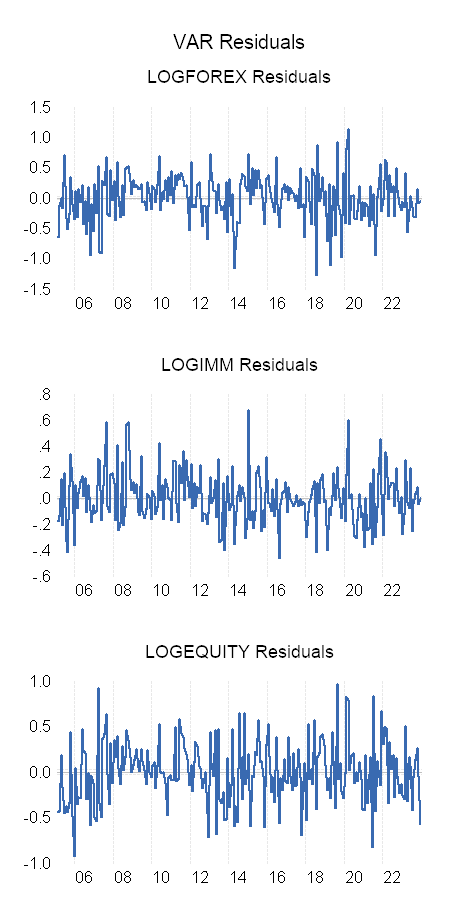
\includegraphics[scale=0.9]{annexes/msih_residuals.png}
    \label{fig:msih_resids}
\end{figure}

\begin{figure}[H]
    \centering
    \caption{Graphique des probabilités de transitions brutes du MSIH-VAR.}
    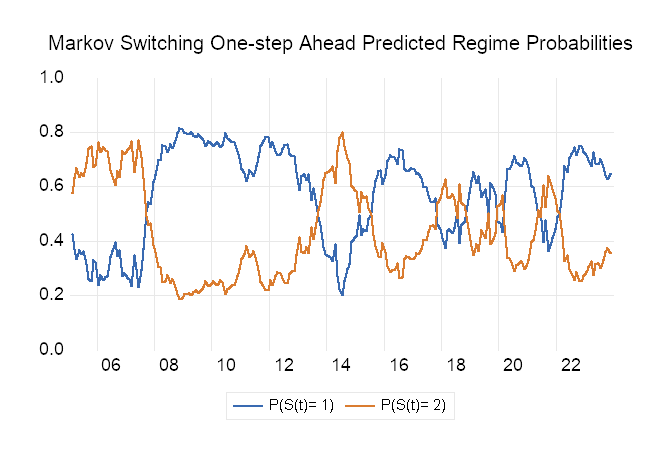
\includegraphics[scale=0.8]{annexes/msih_onestep.png}
    \label{fig:graph_prob_brutes}
\end{figure}

\begin{figure}[H]
    \centering
    \caption{Graphique des probabilités de transitions lisées du MSIH-VAR.}
    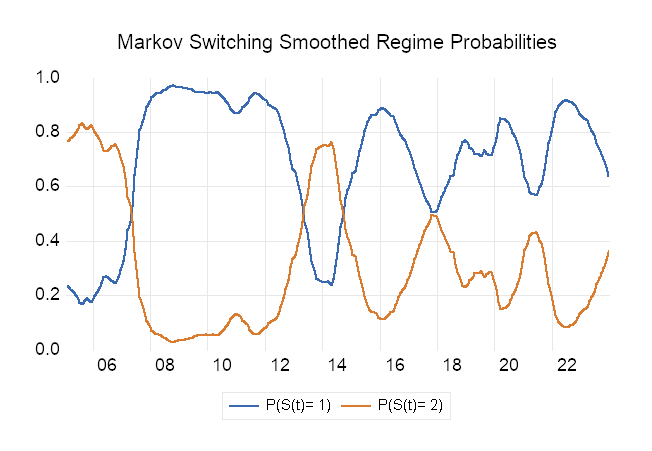
\includegraphics[scale=0.8]{annexes/msih_smoothed.png}
    \label{fig:graph_prob_lissees}
\end{figure}

\begin{table}[H]
    \centering
    \sffamily
    \caption{Test du portmanteau du modèle MISH-VAR.}
    \label{tab:test_portmanteau_var)}
    \resizebox{1\textwidth}{!}{\begin{tabular}{lrrrrr}
\multicolumn{6}{l}{VAR Residual Portmanteau Tests for Autocorrelations}\\
\multicolumn{6}{l}{Null Hypothesis: No residual autocorrelations up to lag h}\\
\multicolumn{3}{l}{Sample: 2005M01 2023M12}&\multicolumn{1}{c}{}&\multicolumn{1}{c}{}&\multicolumn{1}{c}{}\\
\multicolumn{3}{l}{Included observations: 227}&\multicolumn{1}{c}{}&\multicolumn{1}{c}{}&\multicolumn{1}{c}{}\\
[4.5pt] \hline \\ [-4.5pt]
\multicolumn{1}{c}{Lags}&\multicolumn{1}{c}{Q-Stat}&\multicolumn{1}{c}{Prob.*}&\multicolumn{1}{c}{Adj Q-Stat}&\multicolumn{1}{c}{Prob.*}&\multicolumn{1}{c}{df}\\
[4.5pt] \hline \\ [-4.5pt]
\multicolumn{1}{c}{1}&\multicolumn{1}{c}{$6.458256$}&\multicolumn{1}{c}{---}&\multicolumn{1}{c}{$6.486832$}&\multicolumn{1}{c}{---}&\multicolumn{1}{c}{---}\\
\multicolumn{1}{c}{2}&\multicolumn{1}{c}{$18.73100$}&\multicolumn{1}{c}{$0.0276$}&\multicolumn{1}{c}{$18.86867$}&\multicolumn{1}{c}{$0.0263$}&\multicolumn{1}{c}{9}\\
[4.5pt] \hline \\ [-4.5pt]
\multicolumn{6}{l}{*Test is valid only for lags larger than the VAR lag order.}\\
\multicolumn{7}{l}{df is degrees of freedom for (approximate) chi-square distribution}\\
\multicolumn{1}{c}{}&\multicolumn{1}{c}{}&\multicolumn{1}{c}{}&\multicolumn{1}{c}{}&\multicolumn{1}{c}{}&\multicolumn{1}{c}{}\\
\end{tabular}}
\end{table}

\begin{table}[H]
    \centering
    \sffamily
    \caption{Test de normalité du modèle MISH-VAR.}
    \label{tab:test_normalite_var}
    \resizebox{1\textwidth}{!}{\begin{tabular}{lrrrr}
\multicolumn{3}{l}{VAR Residual Normality Tests}&\multicolumn{1}{c}{}&\multicolumn{1}{c}{}\\
\multicolumn{4}{l}{Orthogonalization: Cholesky (Lutkepohl)}&\multicolumn{1}{c}{}\\
\multicolumn{5}{l}{Null Hypothesis: Residuals are multivariate normal}\\
\multicolumn{3}{l}{Sample: 2005M01 2023M12}&\multicolumn{1}{c}{}&\multicolumn{1}{c}{}\\
\multicolumn{3}{l}{Included observations: 227}&\multicolumn{1}{c}{}&\multicolumn{1}{c}{}\\
[4.5pt] \hline \\ [-4.5pt]
\multicolumn{1}{c}{}&\multicolumn{1}{c}{}&\multicolumn{1}{c}{}&\multicolumn{1}{c}{}&\multicolumn{1}{c}{}\\
\multicolumn{1}{c}{Component}&\multicolumn{1}{c}{Jarque-Bera}&\multicolumn{1}{c}{df}&\multicolumn{1}{c}{Prob.}&\multicolumn{1}{c}{}\\
[4.5pt] \hline \\ [-4.5pt]
\multicolumn{1}{c}{1}&\multicolumn{1}{c}{$5.760644$}&\multicolumn{1}{c}{2}&\multicolumn{1}{c}{$0.056117$}&\multicolumn{1}{c}{}\\
\multicolumn{1}{c}{2}&\multicolumn{1}{c}{$1.54375$}&\multicolumn{1}{c}{2}&\multicolumn{1}{c}{$0.4627$}&\multicolumn{1}{c}{}\\
\multicolumn{1}{c}{3}&\multicolumn{1}{c}{$4.746199$}&\multicolumn{1}{c}{2}&\multicolumn{1}{c}{$0.093191$}&\multicolumn{1}{c}{}\\
[4.5pt] \hline \\ [-4.5pt]
\multicolumn{1}{c}{Joint}&\multicolumn{1}{c}{$12.050593$}&\multicolumn{1}{c}{6}&\multicolumn{1}{c}{$0.049$}&\multicolumn{1}{c}{}\\
[4.5pt] \hline \\ [-4.5pt]
\multicolumn{6}{l}{*Approximate p-values do not account for coefficient}\\
\multicolumn{2}{l}{estimation}&\multicolumn{1}{c}{}&\multicolumn{1}{c}{}&\multicolumn{1}{c}{}\\
\multicolumn{1}{c}{}&\multicolumn{1}{c}{}&\multicolumn{1}{c}{}&\multicolumn{1}{c}{}&\multicolumn{1}{c}{}\\
\end{tabular}}
\end{table}

\subsubsection{Décomposition de la variance}

\begin{figure}[H]
    \centering
    \caption{Histogramme de décomposition de la variance du régime 1.}
    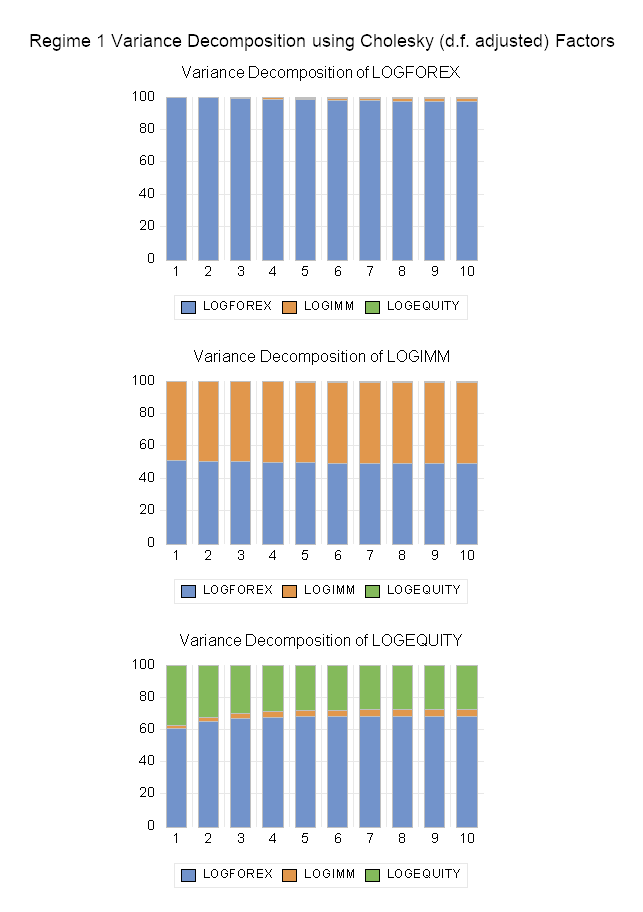
\includegraphics[scale=0.9]{annexes/regime_1.png}
    \label{fig:hist_variance_r1}
\end{figure}

\begin{figure}[H]
    \centering
    \caption{Histogramme de décomposition de la variance du régime 2.}
    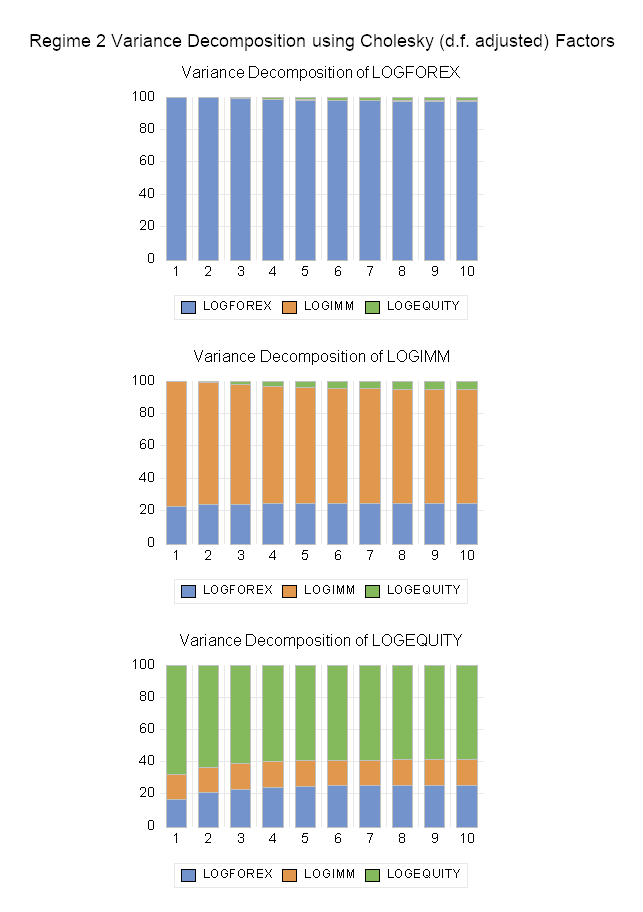
\includegraphics[scale=0.9]{annexes/regime_2.png}
    \label{fig:hist_variance_r2}
\end{figure}

\begin{table}[H]
    \centering
    \sffamily
    \caption{Tableau de décomposition de la variance du modèle 1.}
    \label{tab:tab_variance_r1}
    \resizebox{1\textwidth}{!}{\begin{tabular}{lrrrr}
\multicolumn{1}{c}{Variance Decomposition of LOGFOREX:}&\multicolumn{1}{c}{}&\multicolumn{1}{c}{}&\multicolumn{1}{c}{}&\multicolumn{1}{c}{}\\
\multicolumn{1}{l}{Period}&\multicolumn{1}{c}{S.E.}&\multicolumn{1}{c}{LOGFOREX}&\multicolumn{1}{c}{LOGIMM}&\multicolumn{1}{c}{LOGEQUITY}\\
[4.5pt] \hline \\ [-4.5pt]
\multicolumn{1}{c}{$1$}&\multicolumn{1}{c}{$0.304125$}&\multicolumn{1}{c}{$100.0000$}&\multicolumn{1}{c}{$0.000000$}&\multicolumn{1}{c}{$0.000000$}\\
\multicolumn{1}{c}{$2$}&\multicolumn{1}{c}{$0.364599$}&\multicolumn{1}{c}{$99.65702$}&\multicolumn{1}{c}{$0.139675$}&\multicolumn{1}{c}{$0.203303$}\\
\multicolumn{1}{c}{$3$}&\multicolumn{1}{c}{$0.389700$}&\multicolumn{1}{c}{$99.18205$}&\multicolumn{1}{c}{$0.407331$}&\multicolumn{1}{c}{$0.410614$}\\
\multicolumn{1}{c}{$4$}&\multicolumn{1}{c}{$0.401728$}&\multicolumn{1}{c}{$98.71024$}&\multicolumn{1}{c}{$0.733157$}&\multicolumn{1}{c}{$0.556603$}\\
\multicolumn{1}{c}{$5$}&\multicolumn{1}{c}{$0.408087$}&\multicolumn{1}{c}{$98.29265$}&\multicolumn{1}{c}{$1.060239$}&\multicolumn{1}{c}{$0.647109$}\\
\multicolumn{1}{c}{$6$}&\multicolumn{1}{c}{$0.411728$}&\multicolumn{1}{c}{$97.94471$}&\multicolumn{1}{c}{$1.354747$}&\multicolumn{1}{c}{$0.700546$}\\
\multicolumn{1}{c}{$7$}&\multicolumn{1}{c}{$0.413953$}&\multicolumn{1}{c}{$97.66572$}&\multicolumn{1}{c}{$1.602514$}&\multicolumn{1}{c}{$0.731762$}\\
\multicolumn{1}{c}{$8$}&\multicolumn{1}{c}{$0.415384$}&\multicolumn{1}{c}{$97.44793$}&\multicolumn{1}{c}{$1.801883$}&\multicolumn{1}{c}{$0.750185$}\\
\multicolumn{1}{c}{$9$}&\multicolumn{1}{c}{$0.416338$}&\multicolumn{1}{c}{$97.28114$}&\multicolumn{1}{c}{$1.957564$}&\multicolumn{1}{c}{$0.761296$}\\
\multicolumn{1}{c}{$10$}&\multicolumn{1}{c}{$0.416992$}&\multicolumn{1}{c}{$97.15517$}&\multicolumn{1}{c}{$2.076650$}&\multicolumn{1}{c}{$0.768178$}\\
[4.5pt] \hline \\ [-4.5pt]
\multicolumn{1}{c}{Variance Decomposition of LOGIMM:}&\multicolumn{1}{c}{}&\multicolumn{1}{c}{}&\multicolumn{1}{c}{}&\multicolumn{1}{c}{}\\
\multicolumn{1}{l}{Period}&\multicolumn{1}{c}{S.E.}&\multicolumn{1}{c}{LOGFOREX}&\multicolumn{1}{c}{LOGIMM}&\multicolumn{1}{c}{LOGEQUITY}\\
[4.5pt] \hline \\ [-4.5pt]
\multicolumn{1}{c}{$1$}&\multicolumn{1}{c}{$0.197859$}&\multicolumn{1}{c}{$51.14572$}&\multicolumn{1}{c}{$48.85428$}&\multicolumn{1}{c}{$0.000000$}\\
\multicolumn{1}{c}{$2$}&\multicolumn{1}{c}{$0.258028$}&\multicolumn{1}{c}{$50.52979$}&\multicolumn{1}{c}{$49.25963$}&\multicolumn{1}{c}{$0.210582$}\\
\multicolumn{1}{c}{$3$}&\multicolumn{1}{c}{$0.293564$}&\multicolumn{1}{c}{$50.04328$}&\multicolumn{1}{c}{$49.52211$}&\multicolumn{1}{c}{$0.434615$}\\
\multicolumn{1}{c}{$4$}&\multicolumn{1}{c}{$0.316703$}&\multicolumn{1}{c}{$49.68348$}&\multicolumn{1}{c}{$49.70874$}&\multicolumn{1}{c}{$0.607778$}\\
\multicolumn{1}{c}{$5$}&\multicolumn{1}{c}{$0.332438$}&\multicolumn{1}{c}{$49.42317$}&\multicolumn{1}{c}{$49.84636$}&\multicolumn{1}{c}{$0.730472$}\\
\multicolumn{1}{c}{$6$}&\multicolumn{1}{c}{$0.343393$}&\multicolumn{1}{c}{$49.23600$}&\multicolumn{1}{c}{$49.94878$}&\multicolumn{1}{c}{$0.815218$}\\
\multicolumn{1}{c}{$7$}&\multicolumn{1}{c}{$0.351132$}&\multicolumn{1}{c}{$49.10148$}&\multicolumn{1}{c}{$50.02494$}&\multicolumn{1}{c}{$0.873578$}\\
\multicolumn{1}{c}{$8$}&\multicolumn{1}{c}{$0.356650$}&\multicolumn{1}{c}{$49.00465$}&\multicolumn{1}{c}{$50.08136$}&\multicolumn{1}{c}{$0.913993$}\\
\multicolumn{1}{c}{$9$}&\multicolumn{1}{c}{$0.360608$}&\multicolumn{1}{c}{$48.93479$}&\multicolumn{1}{c}{$50.12299$}&\multicolumn{1}{c}{$0.942215$}\\
\multicolumn{1}{c}{$10$}&\multicolumn{1}{c}{$0.363460$}&\multicolumn{1}{c}{$48.88431$}&\multicolumn{1}{c}{$50.15360$}&\multicolumn{1}{c}{$0.962090$}\\
[4.5pt] \hline \\ [-4.5pt]
\multicolumn{1}{c}{Variance Decomposition of LOGEQUITY:}&\multicolumn{1}{c}{}&\multicolumn{1}{c}{}&\multicolumn{1}{c}{}&\multicolumn{1}{c}{}\\
\multicolumn{1}{l}{Period}&\multicolumn{1}{c}{S.E.}&\multicolumn{1}{c}{LOGFOREX}&\multicolumn{1}{c}{LOGIMM}&\multicolumn{1}{c}{LOGEQUITY}\\
[4.5pt] \hline \\ [-4.5pt]
\multicolumn{1}{c}{$1$}&\multicolumn{1}{c}{$0.218817$}&\multicolumn{1}{c}{$60.27540$}&\multicolumn{1}{c}{$2.020076$}&\multicolumn{1}{c}{$37.70453$}\\
\multicolumn{1}{c}{$2$}&\multicolumn{1}{c}{$0.251373$}&\multicolumn{1}{c}{$64.68915$}&\multicolumn{1}{c}{$2.496150$}&\multicolumn{1}{c}{$32.81470$}\\
\multicolumn{1}{c}{$3$}&\multicolumn{1}{c}{$0.263339$}&\multicolumn{1}{c}{$66.72249$}&\multicolumn{1}{c}{$2.951131$}&\multicolumn{1}{c}{$30.32638$}\\
\multicolumn{1}{c}{$4$}&\multicolumn{1}{c}{$0.268978$}&\multicolumn{1}{c}{$67.55629$}&\multicolumn{1}{c}{$3.360578$}&\multicolumn{1}{c}{$29.08313$}\\
\multicolumn{1}{c}{$5$}&\multicolumn{1}{c}{$0.272064$}&\multicolumn{1}{c}{$67.85628$}&\multicolumn{1}{c}{$3.711987$}&\multicolumn{1}{c}{$28.43173$}\\
\multicolumn{1}{c}{$6$}&\multicolumn{1}{c}{$0.273917$}&\multicolumn{1}{c}{$67.93461$}&\multicolumn{1}{c}{$4.001910$}&\multicolumn{1}{c}{$28.06347$}\\
\multicolumn{1}{c}{$7$}&\multicolumn{1}{c}{$0.275099$}&\multicolumn{1}{c}{$67.92733$}&\multicolumn{1}{c}{$4.233623$}&\multicolumn{1}{c}{$27.83905$}\\
\multicolumn{1}{c}{$8$}&\multicolumn{1}{c}{$0.275885$}&\multicolumn{1}{c}{$67.89177$}&\multicolumn{1}{c}{$4.414314$}&\multicolumn{1}{c}{$27.69391$}\\
\multicolumn{1}{c}{$9$}&\multicolumn{1}{c}{$0.276423$}&\multicolumn{1}{c}{$67.85126$}&\multicolumn{1}{c}{$4.552636$}&\multicolumn{1}{c}{$27.59610$}\\
\multicolumn{1}{c}{$10$}&\multicolumn{1}{c}{$0.276797$}&\multicolumn{1}{c}{$67.81454$}&\multicolumn{1}{c}{$4.657083$}&\multicolumn{1}{c}{$27.52837$}\\
[4.5pt] \hline \\ [-4.5pt]
\multicolumn{3}{l}{Cholesky One S.D. (d.f. adjusted)}&\multicolumn{1}{c}{}&\multicolumn{1}{c}{}\\
\multicolumn{5}{l}{Cholesky ordering:  LOGFOREX LOGIMM LOGEQUITY}\\
[4.5pt] \hline \\ [-4.5pt]
\end{tabular}}
\end{table}

\begin{table}[H]
    \centering
    \sffamily
    \caption{Tableau de décomposition de la variance du modèle 2.}
    \label{tab:tab_variance_r2}
    \resizebox{1\textwidth}{!}{\begin{tabular}{lrrrr}
\multicolumn{1}{c}{Variance Decomposition of LOGFOREX:}&\multicolumn{1}{c}{}&\multicolumn{1}{c}{}&\multicolumn{1}{c}{}&\multicolumn{1}{c}{}\\
\multicolumn{1}{l}{Period}&\multicolumn{1}{c}{S.E.}&\multicolumn{1}{c}{LOGFOREX}&\multicolumn{1}{c}{LOGIMM}&\multicolumn{1}{c}{LOGEQUITY}\\
[4.5pt] \hline \\ [-4.5pt]
\multicolumn{1}{c}{$1$}&\multicolumn{1}{c}{$0.415038$}&\multicolumn{1}{c}{$100.0000$}&\multicolumn{1}{c}{$0.000000$}&\multicolumn{1}{c}{$0.000000$}\\
\multicolumn{1}{c}{$2$}&\multicolumn{1}{c}{$0.496644$}&\multicolumn{1}{c}{$99.45607$}&\multicolumn{1}{c}{$0.005119$}&\multicolumn{1}{c}{$0.538808$}\\
\multicolumn{1}{c}{$3$}&\multicolumn{1}{c}{$0.528972$}&\multicolumn{1}{c}{$98.86155$}&\multicolumn{1}{c}{$0.042531$}&\multicolumn{1}{c}{$1.095918$}\\
\multicolumn{1}{c}{$4$}&\multicolumn{1}{c}{$0.543228$}&\multicolumn{1}{c}{$98.38060$}&\multicolumn{1}{c}{$0.122495$}&\multicolumn{1}{c}{$1.496909$}\\
\multicolumn{1}{c}{$5$}&\multicolumn{1}{c}{$0.549985$}&\multicolumn{1}{c}{$98.01558$}&\multicolumn{1}{c}{$0.232440$}&\multicolumn{1}{c}{$1.751985$}\\
\multicolumn{1}{c}{$6$}&\multicolumn{1}{c}{$0.553427$}&\multicolumn{1}{c}{$97.74044$}&\multicolumn{1}{c}{$0.352838$}&\multicolumn{1}{c}{$1.906723$}\\
\multicolumn{1}{c}{$7$}&\multicolumn{1}{c}{$0.555316$}&\multicolumn{1}{c}{$97.53238$}&\multicolumn{1}{c}{$0.468022$}&\multicolumn{1}{c}{$1.999598$}\\
\multicolumn{1}{c}{$8$}&\multicolumn{1}{c}{$0.556430$}&\multicolumn{1}{c}{$97.37499$}&\multicolumn{1}{c}{$0.569136$}&\multicolumn{1}{c}{$2.055876$}\\
\multicolumn{1}{c}{$9$}&\multicolumn{1}{c}{$0.557128$}&\multicolumn{1}{c}{$97.25634$}&\multicolumn{1}{c}{$0.652985$}&\multicolumn{1}{c}{$2.090672$}\\
\multicolumn{1}{c}{$10$}&\multicolumn{1}{c}{$0.557587$}&\multicolumn{1}{c}{$97.16740$}&\multicolumn{1}{c}{$0.719881$}&\multicolumn{1}{c}{$2.112723$}\\
[4.5pt] \hline \\ [-4.5pt]
\multicolumn{1}{c}{Variance Decomposition of LOGIMM:}&\multicolumn{1}{c}{}&\multicolumn{1}{c}{}&\multicolumn{1}{c}{}&\multicolumn{1}{c}{}\\
\multicolumn{1}{l}{Period}&\multicolumn{1}{c}{S.E.}&\multicolumn{1}{c}{LOGFOREX}&\multicolumn{1}{c}{LOGIMM}&\multicolumn{1}{c}{LOGEQUITY}\\
[4.5pt] \hline \\ [-4.5pt]
\multicolumn{1}{c}{$1$}&\multicolumn{1}{c}{$0.188015$}&\multicolumn{1}{c}{$22.60091$}&\multicolumn{1}{c}{$77.39909$}&\multicolumn{1}{c}{$0.000000$}\\
\multicolumn{1}{c}{$2$}&\multicolumn{1}{c}{$0.243005$}&\multicolumn{1}{c}{$23.58616$}&\multicolumn{1}{c}{$75.24629$}&\multicolumn{1}{c}{$1.167544$}\\
\multicolumn{1}{c}{$3$}&\multicolumn{1}{c}{$0.275579$}&\multicolumn{1}{c}{$23.98151$}&\multicolumn{1}{c}{$73.59318$}&\multicolumn{1}{c}{$2.425316$}\\
\multicolumn{1}{c}{$4$}&\multicolumn{1}{c}{$0.296923$}&\multicolumn{1}{c}{$24.12792$}&\multicolumn{1}{c}{$72.47180$}&\multicolumn{1}{c}{$3.400274$}\\
\multicolumn{1}{c}{$5$}&\multicolumn{1}{c}{$0.311498$}&\multicolumn{1}{c}{$24.17106$}&\multicolumn{1}{c}{$71.73760$}&\multicolumn{1}{c}{$4.091338$}\\
\multicolumn{1}{c}{$6$}&\multicolumn{1}{c}{$0.321669$}&\multicolumn{1}{c}{$24.17293$}&\multicolumn{1}{c}{$71.25840$}&\multicolumn{1}{c}{$4.568664$}\\
\multicolumn{1}{c}{$7$}&\multicolumn{1}{c}{$0.328862$}&\multicolumn{1}{c}{$24.16008$}&\multicolumn{1}{c}{$70.94251$}&\multicolumn{1}{c}{$4.897402$}\\
\multicolumn{1}{c}{$8$}&\multicolumn{1}{c}{$0.333993$}&\multicolumn{1}{c}{$24.14372$}&\multicolumn{1}{c}{$70.73118$}&\multicolumn{1}{c}{$5.125106$}\\
\multicolumn{1}{c}{$9$}&\multicolumn{1}{c}{$0.337674$}&\multicolumn{1}{c}{$24.12827$}&\multicolumn{1}{c}{$70.58757$}&\multicolumn{1}{c}{$5.284153$}\\
\multicolumn{1}{c}{$10$}&\multicolumn{1}{c}{$0.340327$}&\multicolumn{1}{c}{$24.11524$}&\multicolumn{1}{c}{$70.48858$}&\multicolumn{1}{c}{$5.396184$}\\
[4.5pt] \hline \\ [-4.5pt]
\multicolumn{1}{c}{Variance Decomposition of LOGEQUITY:}&\multicolumn{1}{c}{}&\multicolumn{1}{c}{}&\multicolumn{1}{c}{}&\multicolumn{1}{c}{}\\
\multicolumn{1}{l}{Period}&\multicolumn{1}{c}{S.E.}&\multicolumn{1}{c}{LOGFOREX}&\multicolumn{1}{c}{LOGIMM}&\multicolumn{1}{c}{LOGEQUITY}\\
[4.5pt] \hline \\ [-4.5pt]
\multicolumn{1}{c}{$1$}&\multicolumn{1}{c}{$0.360736$}&\multicolumn{1}{c}{$16.42181$}&\multicolumn{1}{c}{$15.35604$}&\multicolumn{1}{c}{$68.22215$}\\
\multicolumn{1}{c}{$2$}&\multicolumn{1}{c}{$0.399543$}&\multicolumn{1}{c}{$20.56477$}&\multicolumn{1}{c}{$15.56026$}&\multicolumn{1}{c}{$63.87498$}\\
\multicolumn{1}{c}{$3$}&\multicolumn{1}{c}{$0.410371$}&\multicolumn{1}{c}{$22.92458$}&\multicolumn{1}{c}{$15.66404$}&\multicolumn{1}{c}{$61.41138$}\\
\multicolumn{1}{c}{$4$}&\multicolumn{1}{c}{$0.414715$}&\multicolumn{1}{c}{$24.10645$}&\multicolumn{1}{c}{$15.73111$}&\multicolumn{1}{c}{$60.16245$}\\
\multicolumn{1}{c}{$5$}&\multicolumn{1}{c}{$0.416914$}&\multicolumn{1}{c}{$24.66861$}&\multicolumn{1}{c}{$15.79222$}&\multicolumn{1}{c}{$59.53917$}\\
\multicolumn{1}{c}{$6$}&\multicolumn{1}{c}{$0.418169$}&\multicolumn{1}{c}{$24.93277$}&\multicolumn{1}{c}{$15.85304$}&\multicolumn{1}{c}{$59.21420$}\\
\multicolumn{1}{c}{$7$}&\multicolumn{1}{c}{$0.418937$}&\multicolumn{1}{c}{$25.05740$}&\multicolumn{1}{c}{$15.91065$}&\multicolumn{1}{c}{$59.03195$}\\
\multicolumn{1}{c}{$8$}&\multicolumn{1}{c}{$0.419429$}&\multicolumn{1}{c}{$25.11669$}&\multicolumn{1}{c}{$15.96169$}&\multicolumn{1}{c}{$58.92162$}\\
\multicolumn{1}{c}{$9$}&\multicolumn{1}{c}{$0.419757$}&\multicolumn{1}{c}{$25.14505$}&\multicolumn{1}{c}{$16.00450$}&\multicolumn{1}{c}{$58.85045$}\\
\multicolumn{1}{c}{$10$}&\multicolumn{1}{c}{$0.419981$}&\multicolumn{1}{c}{$25.15861$}&\multicolumn{1}{c}{$16.03900$}&\multicolumn{1}{c}{$58.80239$}\\
[4.5pt] \hline \\ [-4.5pt]
\multicolumn{3}{l}{Cholesky One S.D. (d.f. adjusted)}&\multicolumn{1}{c}{}&\multicolumn{1}{c}{}\\
\multicolumn{5}{l}{Cholesky ordering:  LOGFOREX LOGIMM LOGEQUITY}\\
[4.5pt] \hline \\ [-4.5pt]
\end{tabular}}
\end{table}

\begin{figure}[H]
    \centering
    \caption{Décomposition historique du régime 2.}
    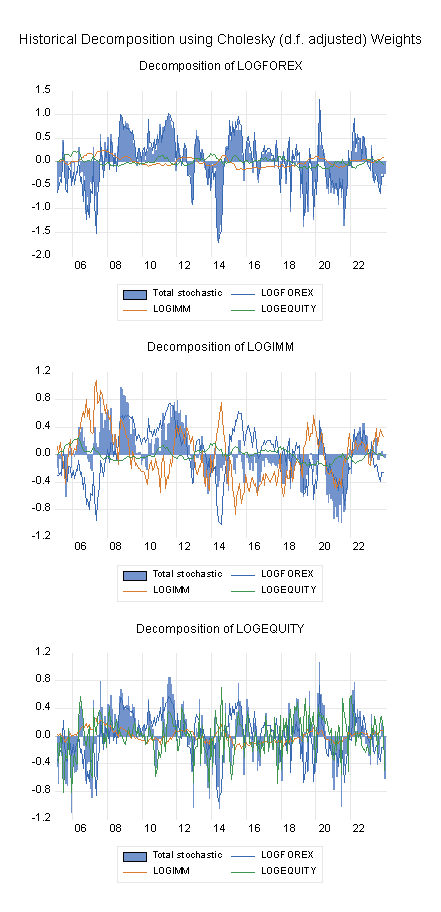
\includegraphics[scale=1]{annexes/regime_1_historcal_decomposition.png}
    \label{fig:msih_resids}
\end{figure}

\begin{figure}[H]
    \centering
    \caption{Décomposition historique du régime 2.}
    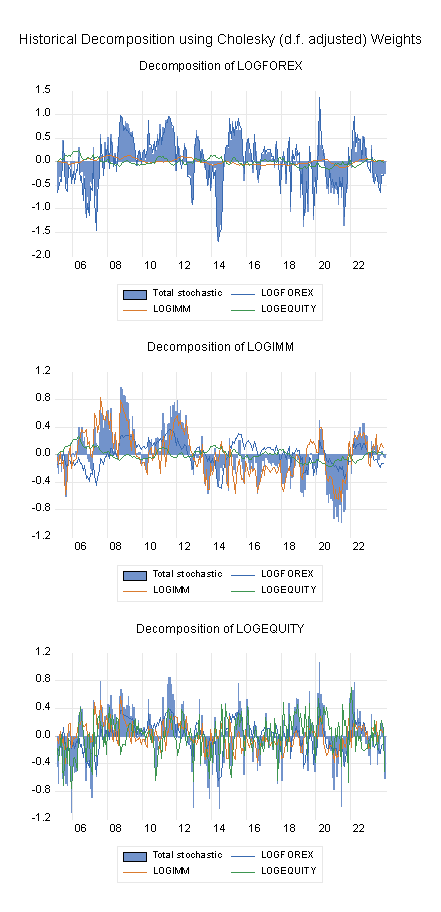
\includegraphics[scale=1]{annexes/regime_2_historical_decomposition.png}
    \label{fig:msih_resids}
\end{figure}

\subsubsection{Fonctions de réponses impulsionnelles}

\begin{figure}[H]
    \centering
    \caption{Réponses impulsionnelles du régime 1.}
    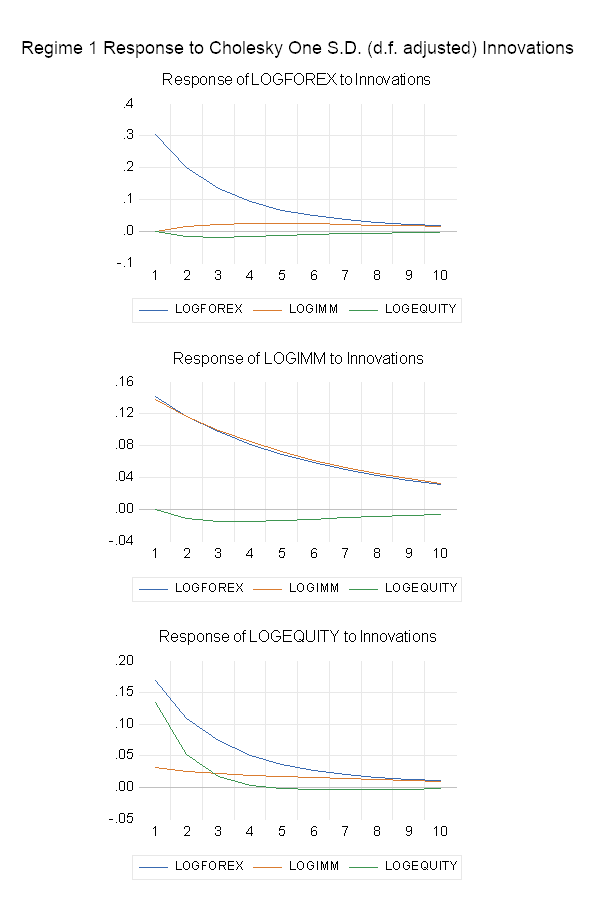
\includegraphics[scale=0.9]{annexes/regime_1_implusereponse.png}
    \label{fig:impulse_reponse_r1}
\end{figure}

\begin{figure}[H]
    \centering
    \caption{Réponses impulsionnelles du régime 2.}
    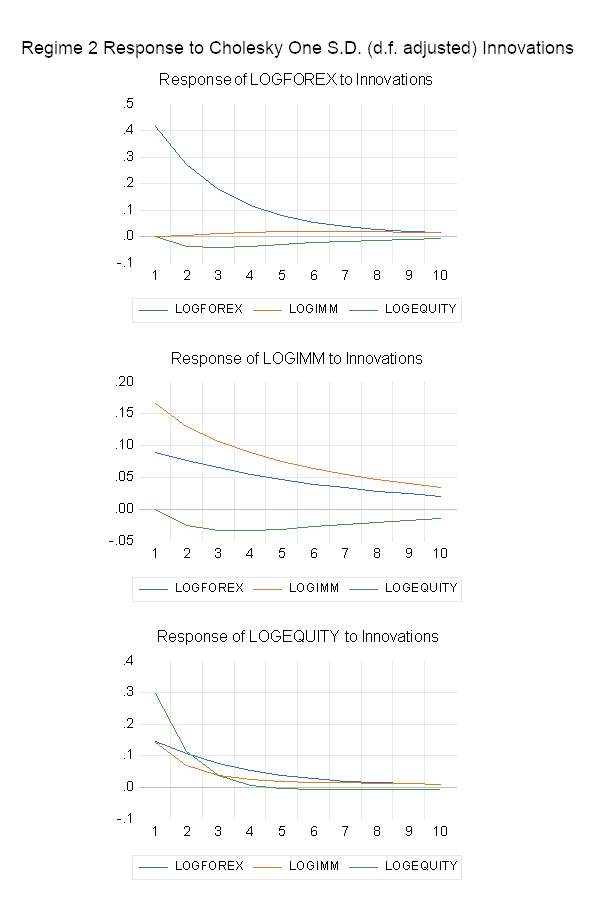
\includegraphics[scale=1]{annexes/regime_2_impulsereponse.png}
    \label{fig:impulse_reponse_r2}
\end{figure}

\begin{figure}[H]
    \centering
    \caption{Réponse impulsionnelle détaillées du régime 1.}
    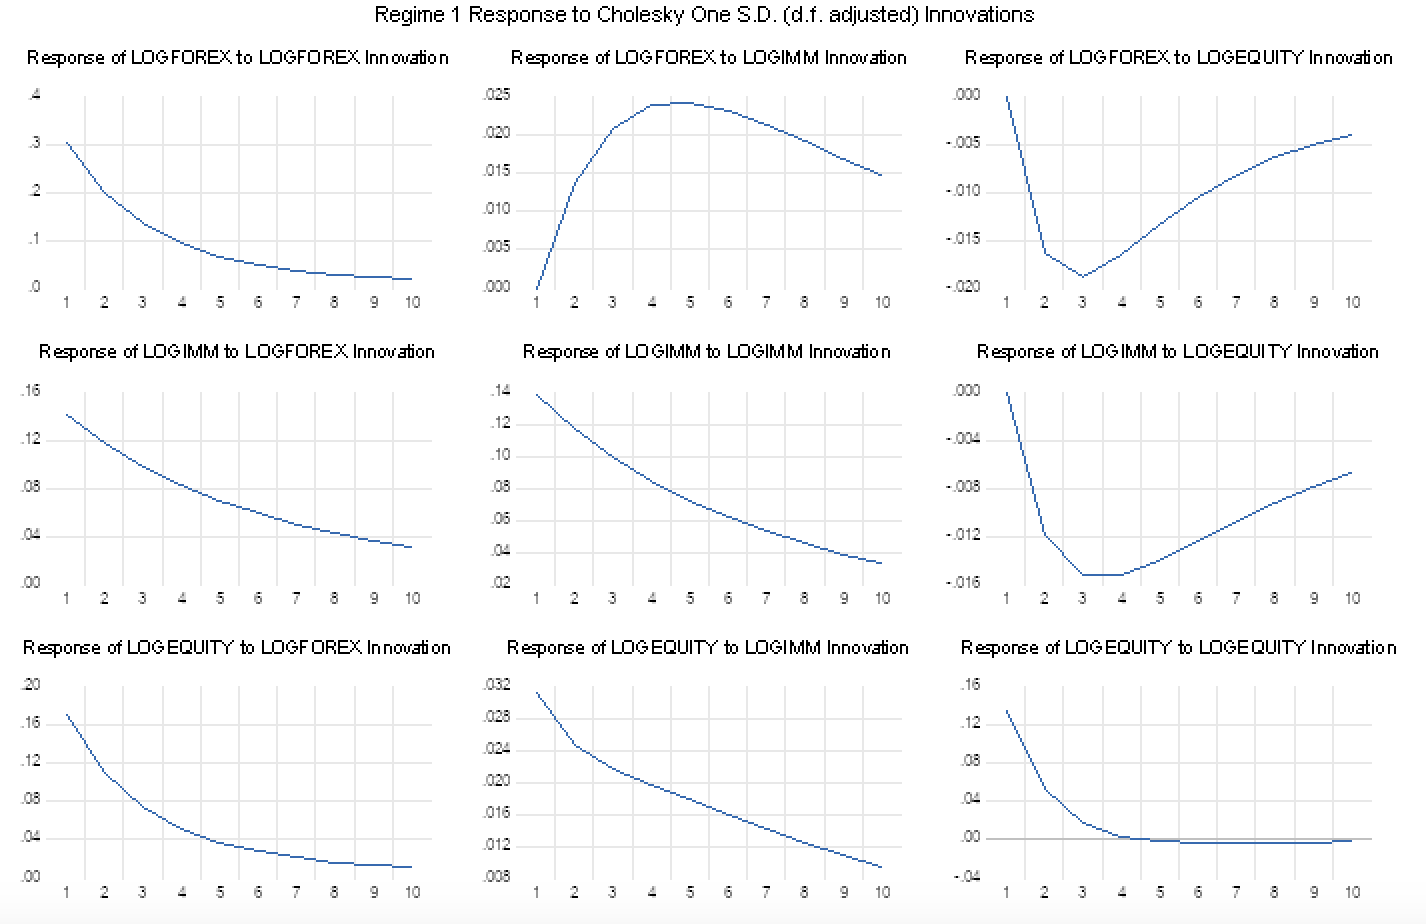
\includegraphics[scale=0.65]{annexes/regime1_mutiple_reponses.png}
    \label{fig:msih_resids}
\end{figure}

\begin{figure}[H]
    \centering
    \caption{Réponse impulsionnelle détaillées du régime 2.}
    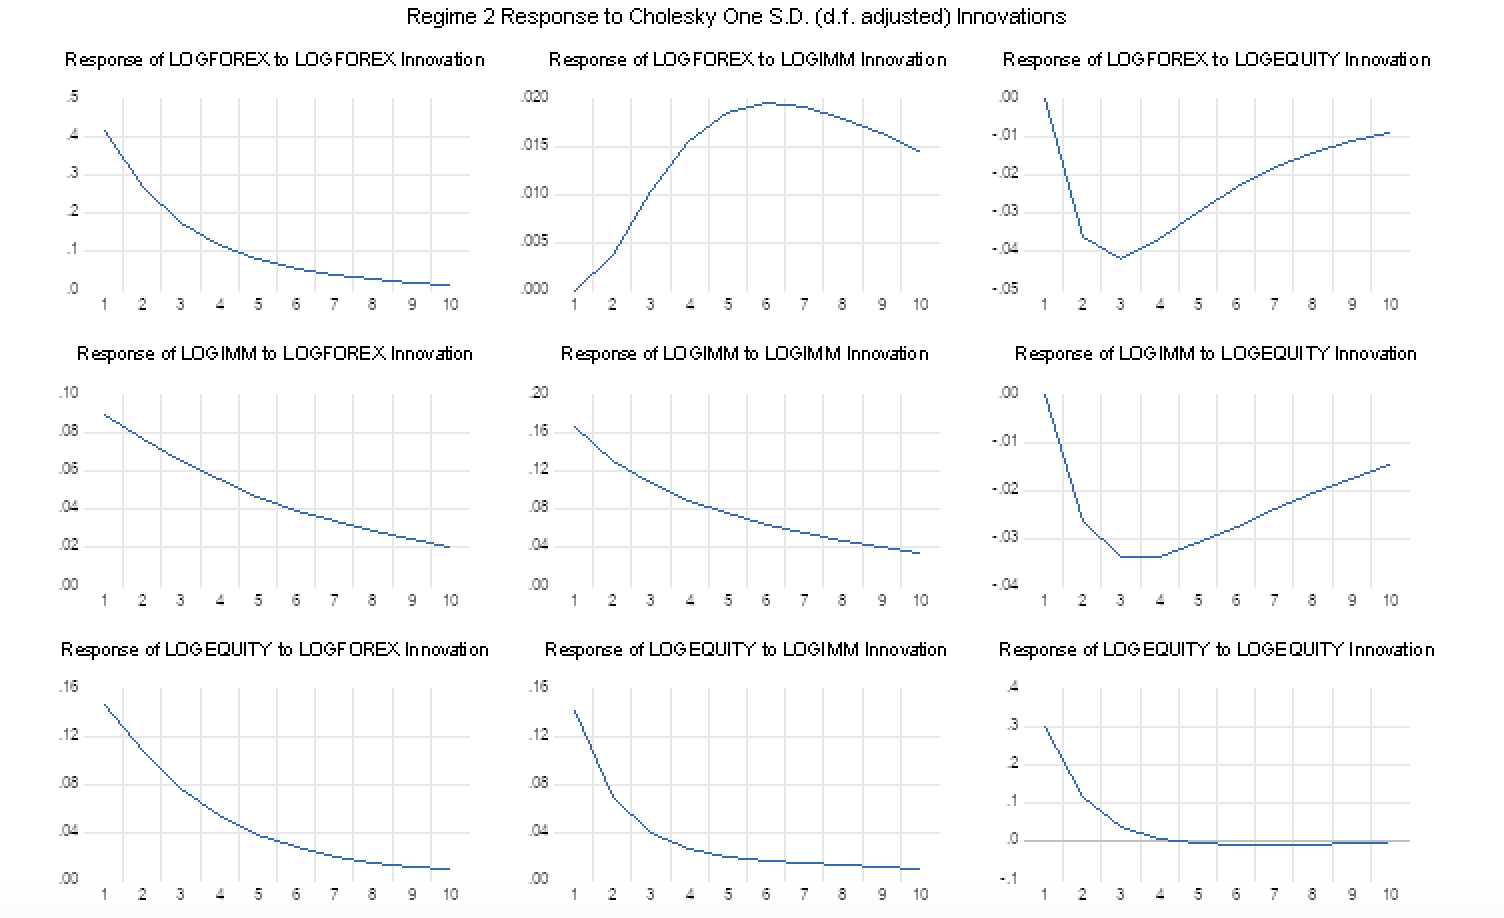
\includegraphics[scale=0.65]{annexes/regime2_multiples_reponses.png}
    \label{fig:msih_resids}
\end{figure}

\subsection{Estimation du modèle NARDL}

\subsubsection{Estimation du modèle NARDL sur le marché interbancaire}

\begin{table}[H]
    \centering
    \sffamily
    \caption{Estimation du modèle NARDL sur le LOGIMM.}
    \label{tab:nardl_logimm}
    \resizebox{1\textwidth}{!}{\begin{tabular}{lrrrr}
\multicolumn{2}{l}{Dependent Variable: LOGIMM}&\multicolumn{1}{c}{}&\multicolumn{1}{c}{}&\multicolumn{1}{c}{}\\
\multicolumn{1}{l}{Method: ARDL}&\multicolumn{1}{c}{}&\multicolumn{1}{c}{}&\multicolumn{1}{c}{}&\multicolumn{1}{c}{}\\
\multicolumn{3}{l}{Sample (adjusted): 2005M04 2023M12}&\multicolumn{1}{c}{}&\multicolumn{1}{c}{}\\
\multicolumn{4}{l}{Included observations: 225 after adjustments}&\multicolumn{1}{c}{}\\
\multicolumn{4}{l}{Maximum dependent lags: 4 (Automatic selection)}&\multicolumn{1}{c}{}\\
\multicolumn{4}{l}{Model selection method: Akaike info criterion (AIC)}&\multicolumn{1}{c}{}\\
\multicolumn{5}{l}{Dynamic regressors : LOGFOREX\_POS}\\
\multicolumn{5}{l}{LOGFOREX\_NEG  LOGEQUITY\_POS LOGEQUITY\_NEG}\\
\multicolumn{1}{l}{Fixed regressors: C}&\multicolumn{1}{c}{}&\multicolumn{1}{c}{}&\multicolumn{1}{c}{}&\multicolumn{1}{c}{}\\
\multicolumn{3}{l}{Number of models evaluated: 2500}&\multicolumn{1}{c}{}&\multicolumn{1}{c}{}\\
\multicolumn{3}{l}{Selected Model: ARDL(3, 1, 0, 1, 1)}&\multicolumn{1}{c}{}&\multicolumn{1}{c}{}\\
\multicolumn{6}{l}{HAC standard errors \& covariance} \\{}&\multicolumn{1}{c}{}&\multicolumn{1}{c}{} \\
[4.5pt] \hline \\ [-4.5pt]
\multicolumn{1}{c}{Variable}&\multicolumn{1}{r}{Coefficient}&\multicolumn{1}{r}{Std. Error}&\multicolumn{1}{r}{t-Statistic}&\multicolumn{1}{r}{Prob.*}\\
[4.5pt] \hline \\ [-4.5pt]
\multicolumn{1}{c}{LOGIMM(-1)}&\multicolumn{1}{r}{$0.838641$}&\multicolumn{1}{r}{$0.059959$}&\multicolumn{1}{r}{$13.98694$}&\multicolumn{1}{r}{$0.0000$}\\
\multicolumn{1}{c}{LOGIMM(-2)}&\multicolumn{1}{r}{$-0.161290$}&\multicolumn{1}{r}{$0.064646$}&\multicolumn{1}{r}{$-2.494978$}&\multicolumn{1}{r}{$0.0134$}\\
\multicolumn{1}{c}{LOGIMM(-3)}&\multicolumn{1}{r}{$0.097142$}&\multicolumn{1}{r}{$0.039186$}&\multicolumn{1}{r}{$2.479022$}&\multicolumn{1}{r}{$0.0139$}\\
\multicolumn{1}{c}{LOGFOREX\_POS}&\multicolumn{1}{r}{$0.313457$}&\multicolumn{1}{r}{$0.052513$}&\multicolumn{1}{r}{$5.969120$}&\multicolumn{1}{r}{$0.0000$}\\
\multicolumn{1}{c}{LOGFOREX\_POS(-1)}&\multicolumn{1}{r}{$-0.216963$}&\multicolumn{1}{r}{$0.046805$}&\multicolumn{1}{r}{$-4.635433$}&\multicolumn{1}{r}{$0.0000$}\\
\multicolumn{1}{c}{LOGFOREX\_NEG}&\multicolumn{1}{r}{$0.072413$}&\multicolumn{1}{r}{$0.024569$}&\multicolumn{1}{r}{$2.947298$}&\multicolumn{1}{r}{$0.0036$}\\
\multicolumn{1}{c}{LOGEQUITY\_POS}&\multicolumn{1}{r}{$0.190579$}&\multicolumn{1}{r}{$0.051848$}&\multicolumn{1}{r}{$3.675710$}&\multicolumn{1}{r}{$0.0003$}\\
\multicolumn{1}{c}{LOGEQUITY\_POS(-1)}&\multicolumn{1}{r}{$-0.127202$}&\multicolumn{1}{r}{$0.044382$}&\multicolumn{1}{r}{$-2.866090$}&\multicolumn{1}{r}{$0.0046$}\\
\multicolumn{1}{c}{LOGEQUITY\_NEG}&\multicolumn{1}{r}{$0.277842$}&\multicolumn{1}{r}{$0.056744$}&\multicolumn{1}{r}{$4.896384$}&\multicolumn{1}{r}{$0.0000$}\\
\multicolumn{1}{c}{LOGEQUITY\_NEG(-1)}&\multicolumn{1}{r}{$-0.185179$}&\multicolumn{1}{r}{$0.067938$}&\multicolumn{1}{r}{$-2.725690$}&\multicolumn{1}{r}{$0.0069$}\\
\multicolumn{1}{c}{C}&\multicolumn{1}{r}{$0.163384$}&\multicolumn{1}{r}{$0.058793$}&\multicolumn{1}{r}{$2.778979$}&\multicolumn{1}{r}{$0.0059$}\\
[4.5pt] \hline \\ [-4.5pt]
\multicolumn{1}{l}{R-squared}&\multicolumn{1}{r}{$0.916264$}&\multicolumn{2}{l}{Mean dependent var}&\multicolumn{1}{r}{$1.363154$}\\
\multicolumn{1}{l}{Adjusted R-squared}&\multicolumn{1}{r}{$0.912351$}&\multicolumn{2}{l}{S.D. dependent var}&\multicolumn{1}{r}{$0.491108$}\\
\multicolumn{1}{l}{S.E. of regression}&\multicolumn{1}{r}{$0.145395$}&\multicolumn{2}{l}{Akaike info criterion}&\multicolumn{1}{r}{$-0.971070$}\\
\multicolumn{1}{l}{Sum squared resid}&\multicolumn{1}{r}{$4.523904$}&\multicolumn{2}{l}{Schwarz criterion}&\multicolumn{1}{r}{$-0.804061$}\\
\multicolumn{1}{l}{Log likelihood}&\multicolumn{1}{r}{$120.2454$}&\multicolumn{2}{l}{Hannan-Quinn criter.}&\multicolumn{1}{r}{$-0.903665$}\\
\multicolumn{1}{l}{F-statistic}&\multicolumn{1}{r}{$234.1656$}&\multicolumn{2}{l}{Durbin-Watson stat}&\multicolumn{1}{r}{$2.019332$}\\
\multicolumn{1}{l}{Prob(F-statistic)}&\multicolumn{1}{r}{$0.000000$}&\multicolumn{1}{c}{}&\multicolumn{1}{c}{}&\multicolumn{1}{c}{}\\
[4.5pt] \hline \\ [-4.5pt]
\multicolumn{1}{l}{selection.}&\multicolumn{1}{c}{}&\multicolumn{1}{c}{}&\multicolumn{1}{c}{}&\multicolumn{1}{c}{}\\
\end{tabular}
}
\end{table}

\begin{table}[H]
    \centering
    \sffamily
    \caption{Test d'existence des asymétries sur le modèle NARDL LOGIMM.}
    \label{tab:asymetrie_nardl_logimm}
    \resizebox{0.8\textwidth}{!}{\begin{tabular}{lrrr}
\multicolumn{1}{l}{Wald Test:}&\multicolumn{1}{c}{}&\multicolumn{1}{c}{}&\multicolumn{1}{c}{}\\
\multicolumn{2}{l}{Equation: NARDL03}&\multicolumn{1}{c}{}&\multicolumn{1}{c}{}\\
[4.5pt] \hline \\ [-4.5pt]
\multicolumn{1}{l}{Test Statistic}&\multicolumn{1}{c}{Value}&\multicolumn{1}{c}{df}&\multicolumn{1}{c}{Probability}\\
[4.5pt] \hline \\ [-4.5pt]
\multicolumn{1}{l}{F-statistic}&\multicolumn{1}{c}{$8.856966$}&\multicolumn{1}{c}{(4, 214)}&\multicolumn{1}{c}{$0.0000$}\\
\multicolumn{1}{l}{Chi-square}&\multicolumn{1}{c}{$35.42787$}&\multicolumn{1}{c}{$4$}&\multicolumn{1}{c}{$0.0000$}\\
[4.5pt] \hline \\ [-4.5pt]
\multicolumn{1}{c}{}&\multicolumn{1}{c}{}&\multicolumn{1}{c}{}&\multicolumn{1}{c}{}\\
\multicolumn{5}{l}{Null Hypothesis: C(4) = C(6), C(5) = 0,}\\
\multicolumn{1}{l}{C(7) = C(9), C(8) =C(10)}&\multicolumn{1}{c}{}&\multicolumn{1}{c}{}&\multicolumn{1}{c}{}\\
\multicolumn{2}{l}{Null Hypothesis Summary:}&\multicolumn{1}{c}{}&\multicolumn{1}{c}{}\\
[4.5pt] \hline \\ [-4.5pt]
\multicolumn{2}{l}{Normalized Restriction (= 0)}&\multicolumn{1}{c}{Value}&\multicolumn{1}{c}{Std. Err.}\\
[4.5pt] \hline \\ [-4.5pt]
\multicolumn{1}{l}{C(4) - C(6)}&\multicolumn{1}{c}{}&\multicolumn{1}{c}{$0.241045$}&\multicolumn{1}{c}{$0.047354$}\\
\multicolumn{1}{l}{C(5)}&\multicolumn{1}{c}{}&\multicolumn{1}{c}{$-0.216963$}&\multicolumn{1}{c}{$0.046805$}\\
\multicolumn{1}{l}{C(7) - C(9)}&\multicolumn{1}{c}{}&\multicolumn{1}{c}{$-0.087263$}&\multicolumn{1}{c}{$0.090034$}\\
\multicolumn{1}{l}{C(8) - C(10)}&\multicolumn{1}{c}{}&\multicolumn{1}{c}{$0.057977$}&\multicolumn{1}{c}{$0.083753$}\\
[4.5pt] \hline \\ [-4.5pt]
\multicolumn{3}{l}{Restrictions are linear in coefficients.}&\multicolumn{1}{c}{}\\
\end{tabular}}
\end{table}

\begin{table}[H]
    \centering
    \sffamily
    \caption{Test de multicolinéarité (VIF) sur le modèle NARDL LOGIMM.}
    \label{tab:vif_nardl_logimm}
    \resizebox{0.8\textwidth}{!}{\begin{tabular}{lrrr}
\multicolumn{2}{l}{Variance Inflation Factors}&\multicolumn{1}{c}{}&\multicolumn{1}{c}{}\\
\multicolumn{2}{l}{Sample: 2005M01 2023M12}&\multicolumn{1}{c}{}&\multicolumn{1}{c}{}\\
\multicolumn{2}{l}{Included observations: 225}&\multicolumn{1}{c}{}&\multicolumn{1}{c}{}\\
[4.5pt] \hline \\ [-4.5pt]
\multicolumn{1}{c}{}&\multicolumn{1}{c}{Coefficient}&\multicolumn{1}{c}{Uncentered}&\multicolumn{1}{c}{Centered}\\
\multicolumn{1}{c}{Variable}&\multicolumn{1}{c}{Variance}&\multicolumn{1}{c}{VIF}&\multicolumn{1}{c}{VIF}\\
[4.5pt] \hline \\ [-4.5pt]
\multicolumn{1}{c}{LOGIMM(-1)}&\multicolumn{1}{c}{$0.003595$}&\multicolumn{1}{c}{$88.95157$}&\multicolumn{1}{c}{$11.45420$}\\
\multicolumn{1}{c}{LOGIMM(-2)}&\multicolumn{1}{c}{$0.004179$}&\multicolumn{1}{c}{$109.1952$}&\multicolumn{1}{c}{$15.65318$}\\
\multicolumn{1}{c}{LOGIMM(-3)}&\multicolumn{1}{c}{$0.001536$}&\multicolumn{1}{c}{$40.86455$}&\multicolumn{1}{c}{$6.780867$}\\
\multicolumn{1}{c}{LOGFOREX\_POS}&\multicolumn{1}{c}{$0.002758$}&\multicolumn{1}{c}{$15347.74$}&\multicolumn{1}{c}{$3607.471$}\\
\multicolumn{1}{c}{LOGFOREX\_POS(-1)}&\multicolumn{1}{c}{$0.002191$}&\multicolumn{1}{c}{$11972.51$}&\multicolumn{1}{c}{$2871.852$}\\
\multicolumn{1}{c}{LOGFOREX\_NEG}&\multicolumn{1}{c}{$0.000604$}&\multicolumn{1}{c}{$3249.708$}&\multicolumn{1}{c}{$807.2229$}\\
\multicolumn{1}{c}{LOGEQUITY\_POS}&\multicolumn{1}{c}{$0.002688$}&\multicolumn{1}{c}{$13237.66$}&\multicolumn{1}{c}{$3119.525$}\\
\multicolumn{1}{c}{LOGEQUITY\_POS(-1)}&\multicolumn{1}{c}{$0.001970$}&\multicolumn{1}{c}{$9509.601$}&\multicolumn{1}{c}{$2272.356$}\\
\multicolumn{1}{c}{LOGEQUITY\_NEG}&\multicolumn{1}{c}{$0.003220$}&\multicolumn{1}{c}{$13849.75$}&\multicolumn{1}{c}{$3687.246$}\\
\multicolumn{1}{c}{LOGEQUITY\_NEG(-1)}&\multicolumn{1}{c}{$0.004616$}&\multicolumn{1}{c}{$19669.81$}&\multicolumn{1}{c}{$5329.415$}\\
\multicolumn{1}{c}{C}&\multicolumn{1}{c}{$0.003457$}&\multicolumn{1}{c}{$47.52094$}&\multicolumn{1}{c}{$NA$}\\
[4.5pt] \hline \\ [-4.5pt]
\end{tabular}}
\end{table}

\begin{table}[H]
    \centering
    \sffamily
    \caption{Test de redondance des variables asymétriques dans le modèle NARDL LOGIMM.}
    \label{tab:redondance_nardl_logimm}
    \resizebox{1\textwidth}{!}{\begin{tabular}{lrrrr}
\multicolumn{2}{l}{Redundant Variables Test}&\multicolumn{1}{c}{}&\multicolumn{1}{c}{}&\multicolumn{1}{c}{}\\
\multicolumn{1}{l}{Equation: NARDL03}&\multicolumn{1}{c}{}&\multicolumn{1}{c}{}&\multicolumn{1}{c}{}&\multicolumn{1}{c}{}\\
\multicolumn{5}{l}{Redundant variables: LOGFOREX\_NEG LOGFOREX\_POS}\\
\multicolumn{5}{l}{LOGEQUITY\_POS LOGEQUITY\_NEG LOGFOREX\_POS(-1)}\\
\multicolumn{4}{l}{LOGEQUITY\_POS(-1) LOGEQUITY\_NEG(-1)}&\multicolumn{1}{c}{}\\
\multicolumn{5}{l}{Specification: LOGIMM LOGIMM(-1) LOGIMM(-2) LOGIMM(-3)}\\
\multicolumn{5}{l}{LOGFOREX\_POS LOGFOREX\_POS(-1) LOGFOREX\_NEG}\\
\multicolumn{5}{l}{LOGEQUITY\_POS LOGEQUITY\_POS(-1) LOGEQUITY\_NEG}\\
\multicolumn{2}{l}{LOGEQUITY\_NEG(-1) C}&\multicolumn{1}{c}{}&\multicolumn{1}{c}{}&\multicolumn{1}{c}{}\\
\multicolumn{6}{l}{Null hypothesis: LOGFOREX\_NEG LOGFOREX\_POS LOGEQUITY\_POS}\\
\multicolumn{6}{l}{LOGEQUITY\_NEG LOGFOREX\_POS(-1) LOGEQUITY\_POS(-1)}\\
\multicolumn{4}{l}{LOGEQUITY\_NEG(-1) are jointly insignificant}&\multicolumn{1}{c}{}\\
[4.5pt] \hline \\ [-4.5pt]
\multicolumn{1}{c}{}&\multicolumn{1}{c}{Value}&\multicolumn{1}{c}{df}&\multicolumn{1}{c}{Probability}&\multicolumn{1}{c}{}\\
\multicolumn{1}{l}{F-statistic}&\multicolumn{1}{c}{$29.94530$}&\multicolumn{1}{c}{(7, 214)}&\multicolumn{1}{c}{$0.0000$}&\multicolumn{1}{c}{}\\
[4.5pt] \hline \\ [-4.5pt]
\multicolumn{1}{l}{F-test summary:}&\multicolumn{1}{c}{}&\multicolumn{1}{c}{}&\multicolumn{1}{c}{}&\multicolumn{1}{c}{}\\
\multicolumn{1}{c}{}&\multicolumn{1}{c}{Sum of Sq.}&\multicolumn{1}{c}{df}&\multicolumn{1}{c}{Mean Squares}&\multicolumn{1}{c}{}\\
\multicolumn{1}{l}{Test SSR}&\multicolumn{1}{c}{$4.431250$}&\multicolumn{1}{c}{$7$}&\multicolumn{1}{c}{$0.633036$}&\multicolumn{1}{c}{}\\
\multicolumn{1}{l}{Restricted SSR}&\multicolumn{1}{c}{$8.955154$}&\multicolumn{1}{c}{$221$}&\multicolumn{1}{c}{$0.040521$}&\multicolumn{1}{c}{}\\
\multicolumn{1}{l}{Unrestricted SSR}&\multicolumn{1}{c}{$4.523904$}&\multicolumn{1}{c}{$214$}&\multicolumn{1}{c}{$0.021140$}&\multicolumn{1}{c}{}\\
[4.5pt] \hline \\ [-4.5pt]
\multicolumn{1}{c}{}&\multicolumn{1}{c}{}&\multicolumn{1}{c}{}&\multicolumn{1}{c}{}&\multicolumn{1}{c}{}\\
\multicolumn{2}{l}{Restricted Test Equation:}&\multicolumn{1}{c}{}&\multicolumn{1}{c}{}&\multicolumn{1}{c}{}\\
\multicolumn{2}{l}{Dependent Variable: LOGIMM}&\multicolumn{1}{c}{}&\multicolumn{1}{c}{}&\multicolumn{1}{c}{}\\
\multicolumn{2}{l}{Method: Least Squares}&\multicolumn{1}{c}{}&\multicolumn{1}{c}{}&\multicolumn{1}{c}{}\\
\multicolumn{2}{l}{Date: 11/12/24   Time: 22:07}&\multicolumn{1}{c}{}&\multicolumn{1}{c}{}&\multicolumn{1}{c}{}\\
\multicolumn{2}{l}{Sample: 2005M04 2023M12}&\multicolumn{1}{c}{}&\multicolumn{1}{c}{}&\multicolumn{1}{c}{}\\
\multicolumn{2}{l}{Included observations: 225}&\multicolumn{1}{c}{}&\multicolumn{1}{c}{}&\multicolumn{1}{c}{}\\
\multicolumn{6}{l}{HAC standard errors \& covariance}\\
\multicolumn{2}{l}{bandwidth = 5.0000)}&\multicolumn{1}{c}{}&\multicolumn{1}{c}{}&\multicolumn{1}{c}{}\\
[4.5pt] \hline \\ [-4.5pt]
\multicolumn{1}{c}{Variable}&\multicolumn{1}{r}{Coefficient}&\multicolumn{1}{r}{Std. Error}&\multicolumn{1}{r}{t-Statistic}&\multicolumn{1}{r}{Prob.}\\
[4.5pt] \hline \\ [-4.5pt]
\multicolumn{1}{c}{LOGIMM(-1)}&\multicolumn{1}{r}{$0.873466$}&\multicolumn{1}{r}{$0.071216$}&\multicolumn{1}{r}{$12.26504$}&\multicolumn{1}{r}{$0.0000$}\\
\multicolumn{1}{c}{LOGIMM(-2)}&\multicolumn{1}{r}{$-0.099342$}&\multicolumn{1}{r}{$0.093865$}&\multicolumn{1}{r}{$-1.058342$}&\multicolumn{1}{r}{$0.2911$}\\
\multicolumn{1}{c}{LOGIMM(-3)}&\multicolumn{1}{r}{$0.147103$}&\multicolumn{1}{r}{$0.057355$}&\multicolumn{1}{r}{$2.564778$}&\multicolumn{1}{r}{$0.0110$}\\
\multicolumn{1}{c}{C}&\multicolumn{1}{r}{$0.111491$}&\multicolumn{1}{r}{$0.036443$}&\multicolumn{1}{r}{$3.059348$}&\multicolumn{1}{r}{$0.0025$}\\
[4.5pt] \hline \\ [-4.5pt]
\multicolumn{1}{l}{R-squared}&\multicolumn{1}{r}{$0.834243$}&\multicolumn{2}{l}{Mean dependent var}&\multicolumn{1}{r}{$1.363154$}\\
\multicolumn{1}{l}{Adjusted R-squared}&\multicolumn{1}{r}{$0.831993$}&\multicolumn{2}{l}{S.D. dependent var}&\multicolumn{1}{r}{$0.491108$}\\
\multicolumn{1}{l}{S.E. of regression}&\multicolumn{1}{r}{$0.201298$}&\multicolumn{2}{l}{Akaike info criterion}&\multicolumn{1}{r}{$-0.350439$}\\
\multicolumn{1}{l}{Sum squared resid}&\multicolumn{1}{r}{$8.955154$}&\multicolumn{2}{l}{Schwarz criterion}&\multicolumn{1}{r}{$-0.289708$}\\
\multicolumn{1}{l}{Log likelihood}&\multicolumn{1}{r}{$43.42434$}&\multicolumn{2}{l}{Hannan-Quinn criter.}&\multicolumn{1}{r}{$-0.325927$}\\
\multicolumn{1}{l}{F-statistic}&\multicolumn{1}{r}{$370.7599$}&\multicolumn{2}{l}{Durbin-Watson stat}&\multicolumn{1}{r}{$1.992899$}\\
\multicolumn{1}{l}{Prob(F-statistic)}&\multicolumn{1}{r}{$0.000000$}&\multicolumn{2}{l}{Wald F-statistic}&\multicolumn{1}{r}{$432.8447$}\\
\multicolumn{1}{l}{Prob(Wald F-statistic)}&\multicolumn{1}{r}{$0.000000$}&\multicolumn{1}{c}{}&\multicolumn{1}{c}{}&\multicolumn{1}{c}{}\\
[4.5pt] \hline \\ [-4.5pt]
\end{tabular}
}
\end{table}

\begin{table}[H]
    \centering
    \sffamily
    \caption{Test RESET de Ramsey dans le modèle NARDL LOGIMM.}
    \label{tab:reset_nardl_logimm}
    \resizebox{1\textwidth}{!}{\begin{tabular}{lrrrr}
\multicolumn{1}{l}{Ramsey RESET Test}&\multicolumn{1}{c}{}&\multicolumn{1}{c}{}&\multicolumn{1}{c}{}&\multicolumn{1}{c}{}\\
\multicolumn{1}{l}{Equation: NARDL03}&\multicolumn{1}{c}{}&\multicolumn{1}{c}{}&\multicolumn{1}{c}{}&\multicolumn{1}{c}{}\\
\multicolumn{3}{l}{Omitted Variables: Squares of fitted values}&\multicolumn{1}{c}{}&\multicolumn{1}{c}{}\\
\multicolumn{5}{l}{Specification: LOGIMM LOGIMM(-1) LOGIMM(-2) LOGIMM(-3)}\\
\multicolumn{5}{l}{LOGFOREX\_POS LOGFOREX\_POS(-1) LOGFOREX\_NEG}\\
\multicolumn{5}{l}{LOGEQUITY\_POS LOGEQUITY\_POS(-1) LOGEQUITY\_NEG}\\
\multicolumn{2}{l}{LOGEQUITY\_NEG(-1) C}&\multicolumn{1}{c}{}&\multicolumn{1}{c}{}&\multicolumn{1}{c}{}\\
[4.5pt] \hline \\ [-4.5pt]
\multicolumn{1}{c}{}&\multicolumn{1}{c}{Value}&\multicolumn{1}{c}{df}&\multicolumn{1}{c}{Probability}&\multicolumn{1}{c}{}\\
\multicolumn{1}{l}{t-statistic}&\multicolumn{1}{c}{$0.816548$}&\multicolumn{1}{c}{$213$}&\multicolumn{1}{c}{$0.4151$}&\multicolumn{1}{c}{}\\
\multicolumn{1}{l}{F-statistic}&\multicolumn{1}{c}{$0.666751$}&\multicolumn{1}{c}{(1, 213)}&\multicolumn{1}{c}{$0.4151$}&\multicolumn{1}{c}{}\\
\multicolumn{1}{l}{Likelihood ratio}&\multicolumn{1}{c}{$0.703214$}&\multicolumn{1}{c}{$1$}&\multicolumn{1}{c}{$0.4017$}&\multicolumn{1}{c}{}\\
[4.5pt] \hline \\ [-4.5pt]
\multicolumn{1}{l}{F-test summary:}&\multicolumn{1}{c}{}&\multicolumn{1}{c}{}&\multicolumn{1}{c}{}&\multicolumn{1}{c}{}\\
\multicolumn{1}{c}{}&\multicolumn{1}{c}{Sum of Sq.}&\multicolumn{1}{c}{df}&\multicolumn{1}{c}{Mean Squares}&\multicolumn{1}{c}{}\\
\multicolumn{1}{l}{Test SSR}&\multicolumn{1}{c}{$0.014117$}&\multicolumn{1}{c}{$1$}&\multicolumn{1}{c}{$0.014117$}&\multicolumn{1}{c}{}\\
\multicolumn{1}{l}{Restricted SSR}&\multicolumn{1}{c}{$4.523904$}&\multicolumn{1}{c}{$214$}&\multicolumn{1}{c}{$0.021140$}&\multicolumn{1}{c}{}\\
\multicolumn{1}{l}{Unrestricted SSR}&\multicolumn{1}{c}{$4.509787$}&\multicolumn{1}{c}{$213$}&\multicolumn{1}{c}{$0.021173$}&\multicolumn{1}{c}{}\\
[4.5pt] \hline \\ [-4.5pt]
\multicolumn{1}{l}{LR test summary:}&\multicolumn{1}{c}{}&\multicolumn{1}{c}{}&\multicolumn{1}{c}{}&\multicolumn{1}{c}{}\\
\multicolumn{1}{c}{}&\multicolumn{1}{c}{Value}&\multicolumn{1}{c}{}&\multicolumn{1}{c}{}&\multicolumn{1}{c}{}\\
\multicolumn{1}{l}{Restricted LogL}&\multicolumn{1}{c}{$120.2454$}&\multicolumn{1}{c}{}&\multicolumn{1}{c}{}&\multicolumn{1}{c}{}\\
\multicolumn{1}{l}{Unrestricted LogL}&\multicolumn{1}{c}{$120.5970$}&\multicolumn{1}{c}{}&\multicolumn{1}{c}{}&\multicolumn{1}{c}{}\\
[4.5pt] \hline \\ [-4.5pt]
\multicolumn{1}{c}{}&\multicolumn{1}{c}{}&\multicolumn{1}{c}{}&\multicolumn{1}{c}{}&\multicolumn{1}{c}{}\\
\multicolumn{2}{l}{Unrestricted Test Equation:}&\multicolumn{1}{c}{}&\multicolumn{1}{c}{}&\multicolumn{1}{c}{}\\
\multicolumn{2}{l}{Dependent Variable: LOGIMM}&\multicolumn{1}{c}{}&\multicolumn{1}{c}{}&\multicolumn{1}{c}{}\\
\multicolumn{2}{l}{Method: Least Squares}&\multicolumn{1}{c}{}&\multicolumn{1}{c}{}&\multicolumn{1}{c}{}\\
\multicolumn{2}{l}{Sample: 2005M04 2023M12}&\multicolumn{1}{c}{}&\multicolumn{1}{c}{}&\multicolumn{1}{c}{}\\
\multicolumn{2}{l}{Included observations: 225}&\multicolumn{1}{c}{}&\multicolumn{1}{c}{}&\multicolumn{1}{c}{}\\
\multicolumn{6}{l}{HAC standard errors \& covariance (Bartlett kernel, Newey-West fixed}\\
\multicolumn{2}{l}{bandwidth = 5.0000)}&\multicolumn{1}{c}{}&\multicolumn{1}{c}{}&\multicolumn{1}{c}{}\\
[4.5pt] \hline \\ [-4.5pt]
\multicolumn{1}{c}{Variable}&\multicolumn{1}{r}{Coefficient}&\multicolumn{1}{r}{Std. Error}&\multicolumn{1}{r}{t-Statistic}&\multicolumn{1}{r}{Prob.}\\
[4.5pt] \hline \\ [-4.5pt]
\multicolumn{1}{c}{LOGIMM(-1)}&\multicolumn{1}{r}{$0.760707$}&\multicolumn{1}{r}{$0.108843$}&\multicolumn{1}{r}{$6.989038$}&\multicolumn{1}{r}{$0.0000$}\\
\multicolumn{1}{c}{LOGIMM(-2)}&\multicolumn{1}{r}{$-0.144983$}&\multicolumn{1}{r}{$0.063447$}&\multicolumn{1}{r}{$-2.285118$}&\multicolumn{1}{r}{$0.0233$}\\
\multicolumn{1}{c}{LOGIMM(-3)}&\multicolumn{1}{r}{$0.086958$}&\multicolumn{1}{r}{$0.039457$}&\multicolumn{1}{r}{$2.203869$}&\multicolumn{1}{r}{$0.0286$}\\
\multicolumn{1}{c}{LOGFOREX\_POS}&\multicolumn{1}{r}{$0.285451$}&\multicolumn{1}{r}{$0.059340$}&\multicolumn{1}{r}{$4.810386$}&\multicolumn{1}{r}{$0.0000$}\\
\multicolumn{1}{c}{LOGFOREX\_POS(-1)}&\multicolumn{1}{r}{$-0.197645$}&\multicolumn{1}{r}{$0.052296$}&\multicolumn{1}{r}{$-3.779336$}&\multicolumn{1}{r}{$0.0002$}\\
\multicolumn{1}{c}{LOGFOREX\_NEG}&\multicolumn{1}{r}{$0.068130$}&\multicolumn{1}{r}{$0.024451$}&\multicolumn{1}{r}{$2.786429$}&\multicolumn{1}{r}{$0.0058$}\\
\multicolumn{1}{c}{LOGEQUITY\_POS}&\multicolumn{1}{r}{$0.177361$}&\multicolumn{1}{r}{$0.053660$}&\multicolumn{1}{r}{$3.305252$}&\multicolumn{1}{r}{$0.0011$}\\
\multicolumn{1}{c}{LOGEQUITY\_POS(-1)}&\multicolumn{1}{r}{$-0.118945$}&\multicolumn{1}{r}{$0.044203$}&\multicolumn{1}{r}{$-2.690908$}&\multicolumn{1}{r}{$0.0077$}\\
\multicolumn{1}{c}{LOGEQUITY\_NEG}&\multicolumn{1}{r}{$0.249173$}&\multicolumn{1}{r}{$0.072024$}&\multicolumn{1}{r}{$3.459598$}&\multicolumn{1}{r}{$0.0007$}\\
\multicolumn{1}{c}{LOGEQUITY\_NEG(-1)}&\multicolumn{1}{r}{$-0.166697$}&\multicolumn{1}{r}{$0.075755$}&\multicolumn{1}{r}{$-2.200471$}&\multicolumn{1}{r}{$0.0288$}\\
\multicolumn{1}{c}{C}&\multicolumn{1}{r}{$0.203650$}&\multicolumn{1}{r}{$0.079829$}&\multicolumn{1}{r}{$2.551081$}&\multicolumn{1}{r}{$0.0114$}\\
\multicolumn{1}{c}{FITTED\textasciicircum 2}&\multicolumn{1}{r}{$0.032891$}&\multicolumn{1}{r}{$0.040964$}&\multicolumn{1}{r}{$0.802917$}&\multicolumn{1}{r}{$0.4229$}\\
[4.5pt] \hline \\ [-4.5pt]
\multicolumn{1}{l}{R-squared}&\multicolumn{1}{r}{$0.916525$}&\multicolumn{2}{l}{Mean dependent var}&\multicolumn{1}{r}{$1.363154$}\\
\multicolumn{1}{l}{Adjusted R-squared}&\multicolumn{1}{r}{$0.912215$}&\multicolumn{2}{l}{S.D. dependent var}&\multicolumn{1}{r}{$0.491108$}\\
\multicolumn{1}{l}{S.E. of regression}&\multicolumn{1}{r}{$0.145508$}&\multicolumn{2}{l}{Akaike info criterion}&\multicolumn{1}{r}{$-0.965307$}\\
\multicolumn{1}{l}{Sum squared resid}&\multicolumn{1}{r}{$4.509787$}&\multicolumn{2}{l}{Schwarz criterion}&\multicolumn{1}{r}{$-0.783115$}\\
\multicolumn{1}{l}{Log likelihood}&\multicolumn{1}{r}{$120.5970$}&\multicolumn{2}{l}{Hannan-Quinn criter.}&\multicolumn{1}{r}{$-0.891773$}\\
\multicolumn{1}{l}{F-statistic}&\multicolumn{1}{r}{$212.6069$}&\multicolumn{2}{l}{Durbin-Watson stat}&\multicolumn{1}{r}{$2.026747$}\\
\multicolumn{1}{l}{Prob(F-statistic)}&\multicolumn{1}{r}{$0.000000$}&\multicolumn{2}{l}{Wald F-statistic}&\multicolumn{1}{r}{$246.3661$}\\
\multicolumn{1}{l}{Prob(Wald F-statistic)}&\multicolumn{1}{r}{$0.000000$}&\multicolumn{1}{c}{}&\multicolumn{1}{c}{}&\multicolumn{1}{c}{}\\
[4.5pt] \hline \\ [-4.5pt]
\end{tabular}
}
\end{table}

\begin{figure}[H]
    \centering
    \caption{Test de CUSUM du modèle NARDL sur le LOGIMM.}
    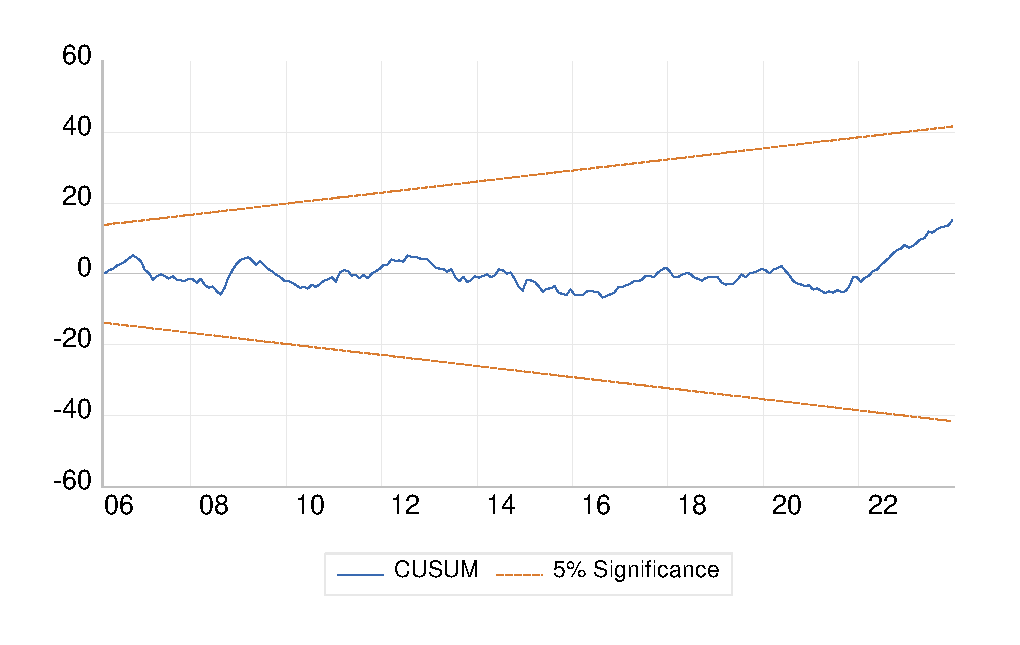
\includegraphics[scale=0.9]{annexes/cusum_nardl_logimm.pdf}
    \label{fig:msih_resids}
\end{figure}

\begin{figure}[H]
    \centering
    \caption{Test de normalité sur les résidus du modèle NARDL sur le LOGIMM.}
    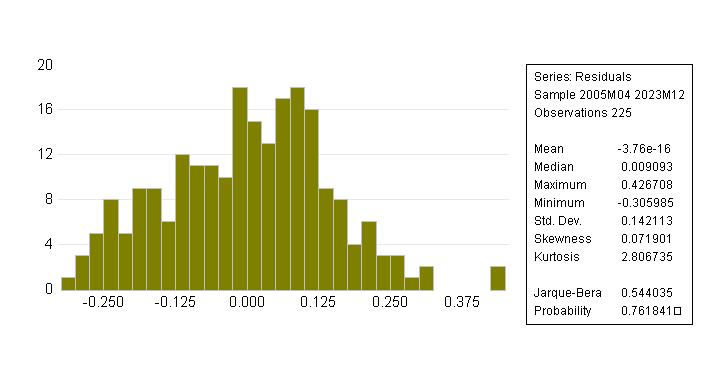
\includegraphics[scale=0.8]{annexes/normality_nardl_logimm.png}
    \label{fig:normalite_nardl_logimm}
\end{figure}

\begin{figure}[H]
    \centering
    \caption{Test d'autorrélation sur les résidus du modèle NARDL sur le LOGIMM.}
    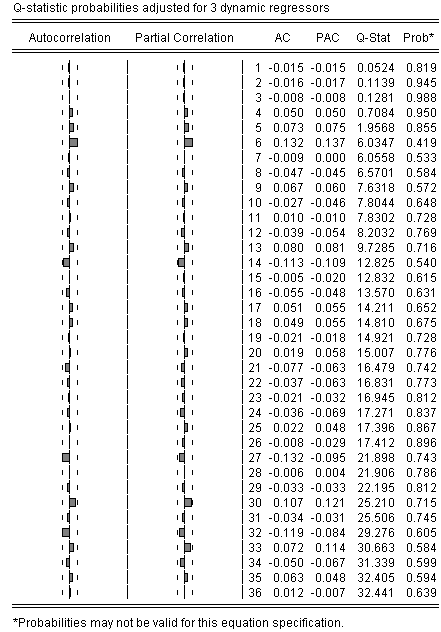
\includegraphics[scale=0.8]{annexes/correlogram_nardl_logimm.png}
    \label{fig:correlo_nardl_imm}
\end{figure}

\begin{table}[H]
    \centering
    \sffamily
    \caption{Test ARCH sur les résidus du modèle NARDL sur le LOGIMM.}
    \label{tab:arch_nardl_logimm}
    \resizebox{0.8\textwidth}{!}{\begin{tabular}{lrrrr}
\multicolumn{2}{l}{Heteroskedasticity Test: ARCH}&\multicolumn{1}{c}{}&\multicolumn{1}{c}{}&\multicolumn{1}{c}{}\\
[4.5pt] \hline \\ [-4.5pt]
\multicolumn{1}{l}{F-statistic}&\multicolumn{1}{r}{$0.398801$}&\multicolumn{2}{l}{Prob. F(10,204)}&\multicolumn{1}{r}{$0.9461$}\\
\multicolumn{1}{l}{Obs*R-squared}&\multicolumn{1}{r}{$4.122461$}&\multicolumn{2}{l}{Prob. Chi-Square(10)}&\multicolumn{1}{r}{$0.9417$}\\
[4.5pt] \hline \\ [-4.5pt]
\multicolumn{1}{c}{}&\multicolumn{1}{c}{}&\multicolumn{1}{c}{}&\multicolumn{1}{c}{}&\multicolumn{1}{c}{}\\
\multicolumn{1}{l}{Test Equation:}&\multicolumn{1}{c}{}&\multicolumn{1}{c}{}&\multicolumn{1}{c}{}&\multicolumn{1}{c}{}\\
\multicolumn{2}{l}{Dependent Variable: RESID\textasciicircum 2}&\multicolumn{1}{c}{}&\multicolumn{1}{c}{}&\multicolumn{1}{c}{}\\
\multicolumn{2}{l}{Method: Least Squares}&\multicolumn{1}{c}{}&\multicolumn{1}{c}{}&\multicolumn{1}{c}{}\\
\multicolumn{3}{l}{Sample (adjusted): 2006M02 2023M12}&\multicolumn{1}{c}{}&\multicolumn{1}{c}{}\\
\multicolumn{4}{l}{Included observations: 215 after adjustments}&\multicolumn{1}{c}{}\\
\multicolumn{6}{l}{HAC standard errors \& covariance}\\
{}&\multicolumn{1}{c}{}&\multicolumn{1}{c}{}\\
[4.5pt] \hline \\ [-4.5pt]
\multicolumn{1}{c}{Variable}&\multicolumn{1}{r}{Coefficient}&\multicolumn{1}{r}{Std. Error}&\multicolumn{1}{r}{t-Statistic}&\multicolumn{1}{r}{Prob.}\\
[4.5pt] \hline \\ [-4.5pt]
\multicolumn{1}{c}{C}&\multicolumn{1}{r}{$0.018258$}&\multicolumn{1}{r}{$0.004048$}&\multicolumn{1}{r}{$4.510838$}&\multicolumn{1}{r}{$0.0000$}\\
\multicolumn{1}{c}{RESID\textasciicircum 2(-1)}&\multicolumn{1}{r}{$0.030943$}&\multicolumn{1}{r}{$0.065730$}&\multicolumn{1}{r}{$0.470754$}&\multicolumn{1}{r}{$0.6383$}\\
\multicolumn{1}{c}{RESID\textasciicircum 2(-2)}&\multicolumn{1}{r}{$0.044582$}&\multicolumn{1}{r}{$0.071457$}&\multicolumn{1}{r}{$0.623905$}&\multicolumn{1}{r}{$0.5334$}\\
\multicolumn{1}{c}{RESID\textasciicircum 2(-3)}&\multicolumn{1}{r}{$0.030183$}&\multicolumn{1}{r}{$0.056093$}&\multicolumn{1}{r}{$0.538087$}&\multicolumn{1}{r}{$0.5911$}\\
\multicolumn{1}{c}{RESID\textasciicircum 2(-4)}&\multicolumn{1}{r}{$0.018190$}&\multicolumn{1}{r}{$0.070288$}&\multicolumn{1}{r}{$0.258790$}&\multicolumn{1}{r}{$0.7961$}\\
\multicolumn{1}{c}{RESID\textasciicircum 2(-5)}&\multicolumn{1}{r}{$0.012319$}&\multicolumn{1}{r}{$0.056729$}&\multicolumn{1}{r}{$0.217151$}&\multicolumn{1}{r}{$0.8283$}\\
\multicolumn{1}{c}{RESID\textasciicircum 2(-6)}&\multicolumn{1}{r}{$-0.009711$}&\multicolumn{1}{r}{$0.060427$}&\multicolumn{1}{r}{$-0.160709$}&\multicolumn{1}{r}{$0.8725$}\\
\multicolumn{1}{c}{RESID\textasciicircum 2(-7)}&\multicolumn{1}{r}{$-0.025220$}&\multicolumn{1}{r}{$0.050909$}&\multicolumn{1}{r}{$-0.495387$}&\multicolumn{1}{r}{$0.6209$}\\
\multicolumn{1}{c}{RESID\textasciicircum 2(-8)}&\multicolumn{1}{r}{$0.079311$}&\multicolumn{1}{r}{$0.071075$}&\multicolumn{1}{r}{$1.115873$}&\multicolumn{1}{r}{$0.2658$}\\
\multicolumn{1}{c}{RESID\textasciicircum 2(-9)}&\multicolumn{1}{r}{$-0.084982$}&\multicolumn{1}{r}{$0.046664$}&\multicolumn{1}{r}{$-1.821152$}&\multicolumn{1}{r}{$0.0700$}\\
\multicolumn{1}{c}{RESID\textasciicircum 2(-10)}&\multicolumn{1}{r}{$-0.023029$}&\multicolumn{1}{r}{$0.049464$}&\multicolumn{1}{r}{$-0.465568$}&\multicolumn{1}{r}{$0.6420$}\\
[4.5pt] \hline \\ [-4.5pt]
\multicolumn{1}{l}{R-squared}&\multicolumn{1}{r}{$0.019174$}&\multicolumn{2}{l}{Mean dependent var}&\multicolumn{1}{r}{$0.019635$}\\
\multicolumn{1}{l}{Adjusted R-squared}&\multicolumn{1}{r}{$-0.028905$}&\multicolumn{2}{l}{S.D. dependent var}&\multicolumn{1}{r}{$0.026870$}\\
\multicolumn{1}{l}{S.E. of regression}&\multicolumn{1}{r}{$0.027255$}&\multicolumn{2}{l}{Akaike info criterion}&\multicolumn{1}{r}{$-4.317326$}\\
\multicolumn{1}{l}{Sum squared resid}&\multicolumn{1}{r}{$0.151542$}&\multicolumn{2}{l}{Schwarz criterion}&\multicolumn{1}{r}{$-4.144874$}\\
\multicolumn{1}{l}{Log likelihood}&\multicolumn{1}{r}{$475.1125$}&\multicolumn{2}{l}{Hannan-Quinn criter.}&\multicolumn{1}{r}{$-4.247647$}\\
\multicolumn{1}{l}{F-statistic}&\multicolumn{1}{r}{$0.398801$}&\multicolumn{2}{l}{Durbin-Watson stat}&\multicolumn{1}{r}{$1.997920$}\\
\multicolumn{1}{l}{Prob(F-statistic)}&\multicolumn{1}{r}{$0.946145$}&\multicolumn{1}{c}{}&\multicolumn{1}{c}{}&\multicolumn{1}{c}{}\\
[4.5pt] \hline \\ [-4.5pt]
\end{tabular}}
\end{table}

\subsubsection{Estimation du modèle NARDL sur le marché actions}

\begin{table}[H]
    \centering
    \sffamily
    \caption{Estimation du modèle NARDL sur le LOGEQUITY.}
    \label{tab:nardl_logequity}
    \resizebox{0.8\textwidth}{!}{\begin{tabular}{lrrrr}
\multicolumn{3}{l}{Dependent Variable: LOGEQUITY}&\multicolumn{1}{c}{}&\multicolumn{1}{c}{}\\
\multicolumn{1}{l}{Method: ARDL}&\multicolumn{1}{c}{}&\multicolumn{1}{c}{}&\multicolumn{1}{c}{}&\multicolumn{1}{c}{}\\
\multicolumn{3}{l}{Sample (adjusted): 2005M06 2023M12}&\multicolumn{1}{c}{}&\multicolumn{1}{c}{}\\
\multicolumn{4}{l}{Included observations: 223 after adjustments}&\multicolumn{1}{c}{}\\
\multicolumn{4}{l}{Maximum dependent lags: 4 (Automatic selection)}&\multicolumn{1}{c}{}\\
\multicolumn{4}{l}{Model selection method: Akaike info criterion (AIC)}&\multicolumn{1}{c}{}\\
\multicolumn{4}{l}{Dynamic regressors : LOGIMM\_POS LOGIMM\_NEG}\\
\multicolumn{3}{l}{LOGFOREX\_POS LOGFOREX\_NEG}&\multicolumn{1}{c}{}&\multicolumn{1}{c}{}\\
\multicolumn{1}{l}{Fixed regressors: C}&\multicolumn{1}{c}{}&\multicolumn{1}{c}{}&\multicolumn{1}{c}{}&\multicolumn{1}{c}{}\\
\multicolumn{3}{l}{Number of models evaluated: 2500}&\multicolumn{1}{c}{}&\multicolumn{1}{c}{}\\
\multicolumn{3}{l}{Selected Model: ARDL(3, 1, 1, 4, 0)}&\multicolumn{1}{c}{}&\multicolumn{1}{c}{}\\
\multicolumn{6}{l}{HAC standard errors \& covariance}\\
\multicolumn{2}{l}{bandwidth = 5.0000)}&\multicolumn{1}{c}{}&\multicolumn{1}{c}{}&\multicolumn{1}{c}{}\\
[4.5pt] \hline \\ [-4.5pt]
\multicolumn{1}{c}{Variable}&\multicolumn{1}{r}{Coefficient}&\multicolumn{1}{r}{Std. Error}&\multicolumn{1}{r}{t-Statistic}&\multicolumn{1}{r}{Prob.*}\\
[4.5pt] \hline \\ [-4.5pt]
\multicolumn{1}{c}{LOGEQUITY(-1)}&\multicolumn{1}{r}{$0.463576$}&\multicolumn{1}{r}{$0.070888$}&\multicolumn{1}{r}{$6.539588$}&\multicolumn{1}{r}{$0.0000$}\\
\multicolumn{1}{c}{LOGEQUITY(-2)}&\multicolumn{1}{r}{$-0.025110$}&\multicolumn{1}{r}{$0.0064991$}&\multicolumn{1}{r}{$-3.86356$}&\multicolumn{1}{r}{$0.0002$}\\
\multicolumn{1}{c}{LOGEQUITY(-3)}&\multicolumn{1}{r}{$0.176925$}&\multicolumn{1}{r}{$0.060576$}&\multicolumn{1}{r}{$2.920687$}&\multicolumn{1}{r}{$0.0039$}\\
\multicolumn{1}{c}{LOGIMM\_POS}&\multicolumn{1}{r}{$0.653087$}&\multicolumn{1}{r}{$0.221923$}&\multicolumn{1}{r}{$2.942849$}&\multicolumn{1}{r}{$0.0036$}\\
\multicolumn{1}{c}{LOGIMM\_POS(-1)}&\multicolumn{1}{r}{$-0.474638$}&\multicolumn{1}{r}{$0.210703$}&\multicolumn{1}{r}{$-2.252646$}&\multicolumn{1}{r}{$0.0253$}\\
\multicolumn{1}{c}{LOGIMM\_NEG}&\multicolumn{1}{r}{$0.809071$}&\multicolumn{1}{r}{$0.175485$}&\multicolumn{1}{r}{$4.610485$}&\multicolumn{1}{r}{$0.0000$}\\
\multicolumn{1}{c}{LOGIMM\_NEG(-1)}&\multicolumn{1}{r}{$-0.617908$}&\multicolumn{1}{r}{$0.168148$}&\multicolumn{1}{r}{$-3.674793$}&\multicolumn{1}{r}{$0.0003$}\\
\multicolumn{1}{c}{LOGFOREX\_POS}&\multicolumn{1}{r}{$0.332573$}&\multicolumn{1}{r}{$0.098151$}&\multicolumn{1}{r}{$3.388394$}&\multicolumn{1}{r}{$0.0008$}\\
\multicolumn{1}{c}{LOGFOREX\_POS(-1)}&\multicolumn{1}{r}{$-0.075632$}&\multicolumn{1}{r}{$0.020755$}&\multicolumn{1}{r}{$-3.644038$}&\multicolumn{1}{r}{$0.0004$}\\
\multicolumn{1}{c}{LOGFOREX\_POS(-2)}&\multicolumn{1}{r}{$0.193545$}&\multicolumn{1}{r}{$0.096894$}&\multicolumn{1}{r}{$1.997487$}&\multicolumn{1}{r}{$0.0471$}\\
\multicolumn{1}{c}{LOGFOREX\_POS(-3)}&\multicolumn{1}{r}{$-0.133520$}&\multicolumn{1}{r}{$0.082747$}&\multicolumn{1}{r}{$-1.613595$}&\multicolumn{1}{r}{$0.1081$}\\
\multicolumn{1}{c}{LOGFOREX\_POS(-4)}&\multicolumn{1}{r}{$-0.099465$}&\multicolumn{1}{r}{$0.049839$}&\multicolumn{1}{r}{$-1.995742$}&\multicolumn{1}{r}{$0.0473$}\\
\multicolumn{1}{c}{LOGFOREX\_NEG}&\multicolumn{1}{r}{$0.207261$}&\multicolumn{1}{r}{$0.044550$}&\multicolumn{1}{r}{$4.652283$}&\multicolumn{1}{r}{$0.0000$}\\
\multicolumn{1}{c}{C}&\multicolumn{1}{r}{$0.364372$}&\multicolumn{1}{r}{$0.126090$}&\multicolumn{1}{r}{$2.889768$}&\multicolumn{1}{r}{$0.0043$}\\
[4.5pt] \hline \\ [-4.5pt]
\multicolumn{1}{l}{R-squared}&\multicolumn{1}{r}{$0.829592$}&\multicolumn{2}{l}{Mean dependent var}&\multicolumn{1}{r}{$1.928245$}\\
\multicolumn{1}{l}{Adjusted R-squared}&\multicolumn{1}{r}{$0.818993$}&\multicolumn{2}{l}{S.D. dependent var}&\multicolumn{1}{r}{$0.606578$}\\
\multicolumn{1}{l}{S.E. of regression}&\multicolumn{1}{r}{$0.258068$}&\multicolumn{2}{l}{Akaike info criterion}&\multicolumn{1}{r}{$0.189539$}\\
\multicolumn{1}{l}{Sum squared resid}&\multicolumn{1}{r}{$13.91925$}&\multicolumn{2}{l}{Schwarz criterion}&\multicolumn{1}{r}{$0.403442$}\\
\multicolumn{1}{l}{Log likelihood}&\multicolumn{1}{r}{$-7.133575$}&\multicolumn{2}{l}{Hannan-Quinn criter.}&\multicolumn{1}{r}{$0.275890$}\\
\multicolumn{1}{l}{F-statistic}&\multicolumn{1}{r}{$78.26701$}&\multicolumn{2}{l}{Durbin-Watson stat}&\multicolumn{1}{r}{$1.910624$}\\
\multicolumn{1}{l}{Prob(F-statistic)}&\multicolumn{1}{r}{$0.000000$}&\multicolumn{1}{c}{}&\multicolumn{1}{c}{}&\multicolumn{1}{c}{}\\
[4.5pt] \hline \\ [-4.5pt]
\multicolumn{1}{l}{selection.}&\multicolumn{1}{c}{}&\multicolumn{1}{c}{}&\multicolumn{1}{c}{}&\multicolumn{1}{c}{}\\
\end{tabular}}
\end{table}

\begin{table}[H]
    \centering
    \sffamily
    \caption{Test d'existence des asymétries sur le modèle NARDL LOGEQUITY.}
    \label{tab:asymetrie_nardl_logequity}
    \resizebox{0.8\textwidth}{!}{\begin{tabular}{lrrr}
\multicolumn{1}{l}{Wald Test:}&\multicolumn{1}{c}{}&\multicolumn{1}{c}{}&\multicolumn{1}{c}{}\\
\multicolumn{2}{l}{Equation: NARDL03}&\multicolumn{1}{c}{}&\multicolumn{1}{c}{}\\
[4.5pt] \hline \\ [-4.5pt]
\multicolumn{1}{l}{Test Statistic}&\multicolumn{1}{c}{Value}&\multicolumn{1}{c}{df}&\multicolumn{1}{c}{Probability}\\
[4.5pt] \hline \\ [-4.5pt]
\multicolumn{1}{l}{F-statistic}&\multicolumn{1}{c}{$3.150231$}&\multicolumn{1}{c}{(7, 209)}&\multicolumn{1}{c}{$0.0035$}\\
\multicolumn{1}{l}{Chi-square}&\multicolumn{1}{c}{$22.05162$}&\multicolumn{1}{c}{$7$}&\multicolumn{1}{c}{$0.0025$}\\
[4.5pt] \hline \\ [-4.5pt]
\multicolumn{1}{c}{}&\multicolumn{1}{c}{}&\multicolumn{1}{c}{}&\multicolumn{1}{c}{}\\
\multicolumn{5}{l}{Null Hypothesis: C(4) = C(9), C(5) = 0, C(6) = 0, C(7) = 0,}\\
\multicolumn{3}{l}{C(8) =0, C(10) = C(12), C(11) = C(13)}&\multicolumn{1}{c}{}\\
\multicolumn{2}{l}{Null Hypothesis Summary:}&\multicolumn{1}{c}{}&\multicolumn{1}{c}{}\\
[4.5pt] \hline \\ [-4.5pt]
\multicolumn{2}{l}{Normalized Restriction (= 0)}&\multicolumn{1}{c}{Value}&\multicolumn{1}{c}{Std. Err.}\\
[4.5pt] \hline \\ [-4.5pt]
\multicolumn{1}{l}{C(4) - C(9)}&\multicolumn{1}{c}{}&\multicolumn{1}{c}{$0.125312$}&\multicolumn{1}{c}{$0.094158$}\\
\multicolumn{1}{l}{C(5)}&\multicolumn{1}{c}{}&\multicolumn{1}{c}{$-0.075632$}&\multicolumn{1}{c}{$0.120755$}\\
\multicolumn{1}{l}{C(6)}&\multicolumn{1}{c}{}&\multicolumn{1}{c}{$0.193545$}&\multicolumn{1}{c}{$0.096894$}\\
\multicolumn{1}{l}{C(7)}&\multicolumn{1}{c}{}&\multicolumn{1}{c}{$-0.133520$}&\multicolumn{1}{c}{$0.082747$}\\
\multicolumn{1}{l}{C(8)}&\multicolumn{1}{c}{}&\multicolumn{1}{c}{$-0.099465$}&\multicolumn{1}{c}{$0.049839$}\\
\multicolumn{1}{l}{C(10) - C(12)}&\multicolumn{1}{c}{}&\multicolumn{1}{c}{$-0.155984$}&\multicolumn{1}{c}{$0.328076$}\\
\multicolumn{1}{l}{C(11) - C(13)}&\multicolumn{1}{c}{}&\multicolumn{1}{c}{$0.143270$}&\multicolumn{1}{c}{$0.318155$}\\
[4.5pt] \hline \\ [-4.5pt]
\multicolumn{3}{l}{Restrictions are linear in coefficients.}&\multicolumn{1}{c}{}\\
\end{tabular}
}
\end{table}

\begin{table}[H]
    \centering
    \sffamily
    \caption{Test de multicolinéarité (VIF) sur le modèle NARDL LOGEQUITY.}
    \label{tab:vif_nardl_logequity}
    \resizebox{0.8\textwidth}{!}{\begin{tabular}{lrrr}
\multicolumn{2}{l}{Variance Inflation Factors}&\multicolumn{1}{c}{}&\multicolumn{1}{c}{}\\
\multicolumn{2}{l}{Sample: 2005M01 2023M12}&\multicolumn{1}{c}{}&\multicolumn{1}{c}{}\\
\multicolumn{2}{l}{Included observations: 223}&\multicolumn{1}{c}{}&\multicolumn{1}{c}{}\\
[4.5pt] \hline \\ [-4.5pt]
\multicolumn{1}{c}{}&\multicolumn{1}{c}{Coefficient}&\multicolumn{1}{c}{Uncentered}&\multicolumn{1}{c}{Centered}\\
\multicolumn{1}{c}{Variable}&\multicolumn{1}{c}{Variance}&\multicolumn{1}{c}{VIF}&\multicolumn{1}{c}{VIF}\\
[4.5pt] \hline \\ [-4.5pt]
\multicolumn{1}{c}{LOGEQUITY(-1)}&\multicolumn{1}{c}{$0.005025$}&\multicolumn{1}{c}{$89.62473$}&\multicolumn{1}{c}{$6.766383$}\\
\multicolumn{1}{c}{LOGEQUITY(-2)}&\multicolumn{1}{c}{$0.004224$}&\multicolumn{1}{c}{$76.78250$}&\multicolumn{1}{c}{$6.779116$}\\
\multicolumn{1}{c}{LOGEQUITY(-3)}&\multicolumn{1}{c}{$0.003669$}&\multicolumn{1}{c}{$62.46960$}&\multicolumn{1}{c}{$4.618255$}\\
\multicolumn{1}{c}{LOGFOREX\_POS}&\multicolumn{1}{c}{$0.009634$}&\multicolumn{1}{c}{$18212.75$}&\multicolumn{1}{c}{$3696.508$}\\
\multicolumn{1}{c}{LOGFOREX\_POS(-1)}&\multicolumn{1}{c}{$0.014582$}&\multicolumn{1}{c}{$27125.81$}&\multicolumn{1}{c}{$5558.469$}\\
\multicolumn{1}{c}{LOGFOREX\_POS(-2)}&\multicolumn{1}{c}{$0.009389$}&\multicolumn{1}{c}{$17230.83$}&\multicolumn{1}{c}{$3570.633$}\\
\multicolumn{1}{c}{LOGFOREX\_POS(-3)}&\multicolumn{1}{c}{$0.006847$}&\multicolumn{1}{c}{$12286.82$}&\multicolumn{1}{c}{$2598.632$}\\
\multicolumn{1}{c}{LOGFOREX\_POS(-4)}&\multicolumn{1}{c}{$0.002484$}&\multicolumn{1}{c}{$4373.763$}&\multicolumn{1}{c}{$954.6576$}\\
\multicolumn{1}{c}{LOGFOREX\_NEG}&\multicolumn{1}{c}{$0.001985$}&\multicolumn{1}{c}{$3632.116$}&\multicolumn{1}{c}{$781.0605$}\\
\multicolumn{1}{c}{LOGIMM\_POS}&\multicolumn{1}{c}{$0.049250$}&\multicolumn{1}{c}{$26700.66$}&\multicolumn{1}{c}{$4457.927$}\\
\multicolumn{1}{c}{LOGIMM\_POS(-1)}&\multicolumn{1}{c}{$0.044396$}&\multicolumn{1}{c}{$23771.50$}&\multicolumn{1}{c}{$4033.966$}\\
\multicolumn{1}{c}{LOGIMM\_NEG}&\multicolumn{1}{c}{$0.030795$}&\multicolumn{1}{c}{$15092.43$}&\multicolumn{1}{c}{$3026.259$}\\
\multicolumn{1}{c}{LOGIMM\_NEG(-1)}&\multicolumn{1}{c}{$0.028274$}&\multicolumn{1}{c}{$13698.95$}&\multicolumn{1}{c}{$2775.918$}\\
\multicolumn{1}{c}{C}&\multicolumn{1}{c}{$0.015899$}&\multicolumn{1}{c}{$67.19360$}&\multicolumn{1}{c}{$NA$}\\
[4.5pt] \hline \\ [-4.5pt]
\end{tabular}}
\end{table}

\begin{table}[H]
    \centering
    \sffamily
    \caption{Test de redondance des variables asymétriques dans le modèle NARDL LOGEQUITY.}
    \label{tab:redondance_nardl_logequity}
    \resizebox{1\textwidth}{!}{\begin{tabular}{lrrrr}
\multicolumn{2}{l}{Redundant Variables Test}&\multicolumn{1}{c}{}&\multicolumn{1}{c}{}&\multicolumn{1}{c}{}\\
\multicolumn{1}{l}{Equation: NARDL03}&\multicolumn{1}{c}{}&\multicolumn{1}{c}{}&\multicolumn{1}{c}{}&\multicolumn{1}{c}{}\\
\multicolumn{5}{l}{Redundant variables: LOGFOREX\_POS LOGFOREX\_POS(-1)}\\
\multicolumn{6}{l}{LOGFOREX\_POS(-2) LOGFOREX\_POS(-3) LOGFOREX\_POS(-4)}\\
\multicolumn{6}{l}{LOGFOREX\_NEG LOGIMM\_POS LOGIMM\_POS(-1) LOGIMM\_NEG}\\
\multicolumn{2}{l}{LOGIMM\_NEG(-1)}&\multicolumn{1}{c}{}&\multicolumn{1}{c}{}&\multicolumn{1}{c}{}\\
\multicolumn{6}{l}{Specification: LOGEQUITY LOGEQUITY(-1) LOGEQUITY(-2) LOGEQUITY(}\\
\multicolumn{6}{l}{-3) LOGFOREX\_POS LOGFOREX\_POS(-1) LOGFOREX\_POS(-2)}\\
\multicolumn{5}{l}{LOGFOREX\_POS(-3) LOGFOREX\_POS(-4) LOGFOREX\_NEG}\\
\multicolumn{6}{l}{LOGIMM\_POS LOGIMM\_POS(-1) LOGIMM\_NEG LOGIMM\_NEG(-1) C}\\
\multicolumn{5}{l}{Null hypothesis: LOGFOREX\_POS LOGFOREX\_POS(-1)}\\
\multicolumn{6}{l}{LOGFOREX\_POS(-2) LOGFOREX\_POS(-3) LOGFOREX\_POS(-4)}\\
\multicolumn{6}{l}{LOGFOREX\_NEG LOGIMM\_POS LOGIMM\_POS(-1) LOGIMM\_NEG}\\
\multicolumn{4}{l}{LOGIMM\_NEG(-1)   are jointly insignificant}&\multicolumn{1}{c}{}\\
[4.5pt] \hline \\ [-4.5pt]
\multicolumn{1}{c}{}&\multicolumn{1}{c}{Value}&\multicolumn{1}{c}{df}&\multicolumn{1}{c}{Probability}&\multicolumn{1}{c}{}\\
\multicolumn{1}{l}{F-statistic}&\multicolumn{1}{c}{$19.49109$}&\multicolumn{1}{c}{(10, 209)}&\multicolumn{1}{c}{$0.0000$}&\multicolumn{1}{c}{}\\
[4.5pt] \hline \\ [-4.5pt]
\multicolumn{1}{l}{F-test summary:}&\multicolumn{1}{c}{}&\multicolumn{1}{c}{}&\multicolumn{1}{c}{}&\multicolumn{1}{c}{}\\
\multicolumn{1}{c}{}&\multicolumn{1}{c}{Sum of Sq.}&\multicolumn{1}{c}{df}&\multicolumn{1}{c}{Mean Squares}&\multicolumn{1}{c}{}\\
\multicolumn{1}{l}{Test SSR}&\multicolumn{1}{c}{$12.98093$}&\multicolumn{1}{c}{$10$}&\multicolumn{1}{c}{$1.298093$}&\multicolumn{1}{c}{}\\
\multicolumn{1}{l}{Restricted SSR}&\multicolumn{1}{c}{$26.90018$}&\multicolumn{1}{c}{$219$}&\multicolumn{1}{c}{$0.122832$}&\multicolumn{1}{c}{}\\
\multicolumn{1}{l}{Unrestricted SSR}&\multicolumn{1}{c}{$13.91925$}&\multicolumn{1}{c}{$209$}&\multicolumn{1}{c}{$0.066599$}&\multicolumn{1}{c}{}\\
[4.5pt] \hline \\ [-4.5pt]
\multicolumn{1}{c}{}&\multicolumn{1}{c}{}&\multicolumn{1}{c}{}&\multicolumn{1}{c}{}&\multicolumn{1}{c}{}\\
\multicolumn{2}{l}{Restricted Test Equation:}&\multicolumn{1}{c}{}&\multicolumn{1}{c}{}&\multicolumn{1}{c}{}\\
\multicolumn{3}{l}{Dependent Variable: LOGEQUITY}&\multicolumn{1}{c}{}&\multicolumn{1}{c}{}\\
\multicolumn{2}{l}{Method: Least Squares}&\multicolumn{1}{c}{}&\multicolumn{1}{c}{}&\multicolumn{1}{c}{}\\
\multicolumn{2}{l}{Sample: 2005M06 2023M12}&\multicolumn{1}{c}{}&\multicolumn{1}{c}{}&\multicolumn{1}{c}{}\\
\multicolumn{2}{l}{Included observations: 223}&\multicolumn{1}{c}{}&\multicolumn{1}{c}{}&\multicolumn{1}{c}{}\\
\multicolumn{6}{l}{HAC standard errors \& covariance (Bartlett kernel, Newey-West fixed}\\
\multicolumn{2}{l}{bandwidth = 5.0000)}&\multicolumn{1}{c}{}&\multicolumn{1}{c}{}&\multicolumn{1}{c}{}\\
[4.5pt] \hline \\ [-4.5pt]
\multicolumn{1}{c}{Variable}&\multicolumn{1}{r}{Coefficient}&\multicolumn{1}{r}{Std. Error}&\multicolumn{1}{r}{t-Statistic}&\multicolumn{1}{r}{Prob.}\\
[4.5pt] \hline \\ [-4.5pt]
\multicolumn{1}{c}{LOGEQUITY(-1)}&\multicolumn{1}{r}{$0.617751$}&\multicolumn{1}{r}{$0.085943$}&\multicolumn{1}{r}{$7.187926$}&\multicolumn{1}{r}{$0.0000$}\\
\multicolumn{1}{c}{LOGEQUITY(-2)}&\multicolumn{1}{r}{$0.088479$}&\multicolumn{1}{r}{$0.087108$}&\multicolumn{1}{r}{$1.015741$}&\multicolumn{1}{r}{$0.3109$}\\
\multicolumn{1}{c}{LOGEQUITY(-3)}&\multicolumn{1}{r}{$0.157484$}&\multicolumn{1}{r}{$0.066559$}&\multicolumn{1}{r}{$2.366097$}&\multicolumn{1}{r}{$0.0188$}\\
\multicolumn{1}{c}{C}&\multicolumn{1}{r}{$0.265545$}&\multicolumn{1}{r}{$0.078284$}&\multicolumn{1}{r}{$3.392089$}&\multicolumn{1}{r}{$0.0008$}\\
[4.5pt] \hline \\ [-4.5pt]
\multicolumn{1}{l}{R-squared}&\multicolumn{1}{r}{$0.670672$}&\multicolumn{2}{l}{Mean dependent var}&\multicolumn{1}{r}{$1.928245$}\\
\multicolumn{1}{l}{Adjusted R-squared}&\multicolumn{1}{r}{$0.666161$}&\multicolumn{2}{l}{S.D. dependent var}&\multicolumn{1}{r}{$0.606578$}\\
\multicolumn{1}{l}{S.E. of regression}&\multicolumn{1}{r}{$0.350474$}&\multicolumn{2}{l}{Akaike info criterion}&\multicolumn{1}{r}{$0.758713$}\\
\multicolumn{1}{l}{Sum squared resid}&\multicolumn{1}{r}{$26.90018$}&\multicolumn{2}{l}{Schwarz criterion}&\multicolumn{1}{r}{$0.819828$}\\
\multicolumn{1}{l}{Log likelihood}&\multicolumn{1}{r}{$-80.59648$}&\multicolumn{2}{l}{Hannan-Quinn criter.}&\multicolumn{1}{r}{$0.783385$}\\
\multicolumn{1}{l}{F-statistic}&\multicolumn{1}{r}{$148.6637$}&\multicolumn{2}{l}{Durbin-Watson stat}&\multicolumn{1}{r}{$1.964152$}\\
\multicolumn{1}{l}{Prob(F-statistic)}&\multicolumn{1}{r}{$0.000000$}&\multicolumn{2}{l}{Wald F-statistic}&\multicolumn{1}{r}{$203.4881$}\\
\multicolumn{1}{l}{Prob(Wald F-statistic)}&\multicolumn{1}{r}{$0.000000$}&\multicolumn{1}{c}{}&\multicolumn{1}{c}{}&\multicolumn{1}{c}{}\\
[4.5pt] \hline \\ [-4.5pt]
\end{tabular}
}
\end{table}

\begin{table}[H]
    \centering
    \sffamily
    \caption{Test RESET de Ramsey dans le modèle NARDL LOGEQUITY.}
    \label{tab:reset_nardl_logequity}
    \resizebox{1\textwidth}{!}{\begin{tabular}{lrrrr}
\multicolumn{1}{l}{Ramsey RESET Test}&\multicolumn{1}{c}{}&\multicolumn{1}{c}{}&\multicolumn{1}{c}{}&\multicolumn{1}{c}{}\\
\multicolumn{1}{l}{Equation: NARDL03}&\multicolumn{1}{c}{}&\multicolumn{1}{c}{}&\multicolumn{1}{c}{}&\multicolumn{1}{c}{}\\
\multicolumn{3}{l}{Omitted Variables: Squares of fitted values}&\multicolumn{1}{c}{}&\multicolumn{1}{c}{}\\
\multicolumn{6}{l}{Specification: LOGEQUITY LOGEQUITY(-1) LOGEQUITY(-2) LOGEQUITY(}\\
\multicolumn{6}{l}{-3) LOGFOREX\_POS LOGFOREX\_POS(-1) LOGFOREX\_POS(-2)}\\
\multicolumn{5}{l}{LOGFOREX\_POS(-3) LOGFOREX\_POS(-4) LOGFOREX\_NEG}\\
\multicolumn{6}{l}{LOGIMM\_POS LOGIMM\_POS(-1) LOGIMM\_NEG LOGIMM\_NEG(-1) C}\\
[4.5pt] \hline \\ [-4.5pt]
\multicolumn{1}{c}{}&\multicolumn{1}{c}{Value}&\multicolumn{1}{c}{df}&\multicolumn{1}{c}{Probability}&\multicolumn{1}{c}{}\\
\multicolumn{1}{l}{t-statistic}&\multicolumn{1}{c}{$0.727348$}&\multicolumn{1}{c}{$208$}&\multicolumn{1}{c}{$0.4678$}&\multicolumn{1}{c}{}\\
\multicolumn{1}{l}{F-statistic}&\multicolumn{1}{c}{$0.529035$}&\multicolumn{1}{c}{(1, 208)}&\multicolumn{1}{c}{$0.4678$}&\multicolumn{1}{c}{}\\
\multicolumn{1}{l}{Likelihood ratio}&\multicolumn{1}{c}{$0.566466$}&\multicolumn{1}{c}{$1$}&\multicolumn{1}{c}{$0.4517$}&\multicolumn{1}{c}{}\\
[4.5pt] \hline \\ [-4.5pt]
\multicolumn{1}{l}{F-test summary:}&\multicolumn{1}{c}{}&\multicolumn{1}{c}{}&\multicolumn{1}{c}{}&\multicolumn{1}{c}{}\\
\multicolumn{1}{c}{}&\multicolumn{1}{c}{Sum of Sq.}&\multicolumn{1}{c}{df}&\multicolumn{1}{c}{Mean Squares}&\multicolumn{1}{c}{}\\
\multicolumn{1}{l}{Test SSR}&\multicolumn{1}{c}{$0.035313$}&\multicolumn{1}{c}{$1$}&\multicolumn{1}{c}{$0.035313$}&\multicolumn{1}{c}{}\\
\multicolumn{1}{l}{Restricted SSR}&\multicolumn{1}{c}{$13.91925$}&\multicolumn{1}{c}{$209$}&\multicolumn{1}{c}{$0.066599$}&\multicolumn{1}{c}{}\\
\multicolumn{1}{l}{Unrestricted SSR}&\multicolumn{1}{c}{$13.88394$}&\multicolumn{1}{c}{$208$}&\multicolumn{1}{c}{$0.066750$}&\multicolumn{1}{c}{}\\
[4.5pt] \hline \\ [-4.5pt]
\multicolumn{1}{l}{LR test summary:}&\multicolumn{1}{c}{}&\multicolumn{1}{c}{}&\multicolumn{1}{c}{}&\multicolumn{1}{c}{}\\
\multicolumn{1}{c}{}&\multicolumn{1}{c}{Value}&\multicolumn{1}{c}{}&\multicolumn{1}{c}{}&\multicolumn{1}{c}{}\\
\multicolumn{1}{l}{Restricted LogL}&\multicolumn{1}{c}{$-7.133575$}&\multicolumn{1}{c}{}&\multicolumn{1}{c}{}&\multicolumn{1}{c}{}\\
\multicolumn{1}{l}{Unrestricted LogL}&\multicolumn{1}{c}{$-6.850342$}&\multicolumn{1}{c}{}&\multicolumn{1}{c}{}&\multicolumn{1}{c}{}\\
[4.5pt] \hline \\ [-4.5pt]
\multicolumn{1}{c}{}&\multicolumn{1}{c}{}&\multicolumn{1}{c}{}&\multicolumn{1}{c}{}&\multicolumn{1}{c}{}\\
\multicolumn{2}{l}{Unrestricted Test Equation:}&\multicolumn{1}{c}{}&\multicolumn{1}{c}{}&\multicolumn{1}{c}{}\\
\multicolumn{3}{l}{Dependent Variable: LOGEQUITY}&\multicolumn{1}{c}{}&\multicolumn{1}{c}{}\\
\multicolumn{2}{l}{Method: Least Squares}&\multicolumn{1}{c}{}&\multicolumn{1}{c}{}&\multicolumn{1}{c}{}\\
\multicolumn{2}{l}{Sample: 2005M06 2023M12}&\multicolumn{1}{c}{}&\multicolumn{1}{c}{}&\multicolumn{1}{c}{}\\
\multicolumn{2}{l}{Included observations: 223}&\multicolumn{1}{c}{}&\multicolumn{1}{c}{}&\multicolumn{1}{c}{}\\
\multicolumn{6}{l}{HAC standard errors \& covariance (Bartlett kernel, Newey-West fixed}\\
\multicolumn{2}{l}{bandwidth = 5.0000)}&\multicolumn{1}{c}{}&\multicolumn{1}{c}{}&\multicolumn{1}{c}{}\\
[4.5pt] \hline \\ [-4.5pt]
\multicolumn{1}{c}{Variable}&\multicolumn{1}{r}{Coefficient}&\multicolumn{1}{r}{Std. Error}&\multicolumn{1}{r}{t-Statistic}&\multicolumn{1}{r}{Prob.}\\
[4.5pt] \hline \\ [-4.5pt]
\multicolumn{1}{c}{LOGEQUITY(-1)}&\multicolumn{1}{r}{$0.529799$}&\multicolumn{1}{r}{$0.135150$}&\multicolumn{1}{r}{$3.920087$}&\multicolumn{1}{r}{$0.0001$}\\
\multicolumn{1}{c}{LOGEQUITY(-2)}&\multicolumn{1}{r}{$-0.021647$}&\multicolumn{1}{r}{$0.065149$}&\multicolumn{1}{r}{$-0.332273$}&\multicolumn{1}{r}{$0.7400$}\\
\multicolumn{1}{c}{LOGEQUITY(-3)}&\multicolumn{1}{r}{$0.201077$}&\multicolumn{1}{r}{$0.073221$}&\multicolumn{1}{r}{$2.746183$}&\multicolumn{1}{r}{$0.0066$}\\
\multicolumn{1}{c}{LOGFOREX\_POS}&\multicolumn{1}{r}{$0.374842$}&\multicolumn{1}{r}{$0.129600$}&\multicolumn{1}{r}{$2.892291$}&\multicolumn{1}{r}{$0.0042$}\\
\multicolumn{1}{c}{LOGFOREX\_POS(-1)}&\multicolumn{1}{r}{$-0.076820$}&\multicolumn{1}{r}{$0.120696$}&\multicolumn{1}{r}{$-0.636479$}&\multicolumn{1}{r}{$0.5252$}\\
\multicolumn{1}{c}{LOGFOREX\_POS(-2)}&\multicolumn{1}{r}{$0.218708$}&\multicolumn{1}{r}{$0.103135$}&\multicolumn{1}{r}{$2.120597$}&\multicolumn{1}{r}{$0.0351$}\\
\multicolumn{1}{c}{LOGFOREX\_POS(-3)}&\multicolumn{1}{r}{$-0.154715$}&\multicolumn{1}{r}{$0.084917$}&\multicolumn{1}{r}{$-1.821954$}&\multicolumn{1}{r}{$0.0699$}\\
\multicolumn{1}{c}{LOGFOREX\_POS(-4)}&\multicolumn{1}{r}{$-0.114218$}&\multicolumn{1}{r}{$0.054508$}&\multicolumn{1}{r}{$-2.095447$}&\multicolumn{1}{r}{$0.0373$}\\
\multicolumn{1}{c}{LOGFOREX\_NEG}&\multicolumn{1}{r}{$0.234729$}&\multicolumn{1}{r}{$0.072677$}&\multicolumn{1}{r}{$3.229769$}&\multicolumn{1}{r}{$0.0014$}\\
\multicolumn{1}{c}{LOGIMM\_POS}&\multicolumn{1}{r}{$0.785374$}&\multicolumn{1}{r}{$0.299047$}&\multicolumn{1}{r}{$2.626258$}&\multicolumn{1}{r}{$0.0093$}\\
\multicolumn{1}{c}{LOGIMM\_POS(-1)}&\multicolumn{1}{r}{$-0.569314$}&\multicolumn{1}{r}{$0.274158$}&\multicolumn{1}{r}{$-2.076589$}&\multicolumn{1}{r}{$0.0391$}\\
\multicolumn{1}{c}{LOGIMM\_NEG}&\multicolumn{1}{r}{$0.934707$}&\multicolumn{1}{r}{$0.225839$}&\multicolumn{1}{r}{$4.138816$}&\multicolumn{1}{r}{$0.0001$}\\
\multicolumn{1}{c}{LOGIMM\_NEG(-1)}&\multicolumn{1}{r}{$-0.700899$}&\multicolumn{1}{r}{$0.202031$}&\multicolumn{1}{r}{$-3.469275$}&\multicolumn{1}{r}{$0.0006$}\\
\multicolumn{1}{c}{C}&\multicolumn{1}{r}{$0.290914$}&\multicolumn{1}{r}{$0.168282$}&\multicolumn{1}{r}{$1.728729$}&\multicolumn{1}{r}{$0.0853$}\\
\multicolumn{1}{c}{FITTED\textasciicircum 2}&\multicolumn{1}{r}{$-0.041553$}&\multicolumn{1}{r}{$0.064154$}&\multicolumn{1}{r}{$-0.647702$}&\multicolumn{1}{r}{$0.5179$}\\
[4.5pt] \hline \\ [-4.5pt]
\multicolumn{1}{l}{R-squared}&\multicolumn{1}{r}{$0.830025$}&\multicolumn{2}{l}{Mean dependent var}&\multicolumn{1}{r}{$1.928245$}\\
\multicolumn{1}{l}{Adjusted R-squared}&\multicolumn{1}{r}{$0.818584$}&\multicolumn{2}{l}{S.D. dependent var}&\multicolumn{1}{r}{$0.606578$}\\
\multicolumn{1}{l}{S.E. of regression}&\multicolumn{1}{r}{$0.258360$}&\multicolumn{2}{l}{Akaike info criterion}&\multicolumn{1}{r}{$0.195967$}\\
\multicolumn{1}{l}{Sum squared resid}&\multicolumn{1}{r}{$13.88394$}&\multicolumn{2}{l}{Schwarz criterion}&\multicolumn{1}{r}{$0.425149$}\\
\multicolumn{1}{l}{Log likelihood}&\multicolumn{1}{r}{$-6.850342$}&\multicolumn{2}{l}{Hannan-Quinn criter.}&\multicolumn{1}{r}{$0.288486$}\\
\multicolumn{1}{l}{F-statistic}&\multicolumn{1}{r}{$72.55053$}&\multicolumn{2}{l}{Durbin-Watson stat}&\multicolumn{1}{r}{$1.905886$}\\
\multicolumn{1}{l}{Prob(F-statistic)}&\multicolumn{1}{r}{$0.000000$}&\multicolumn{2}{l}{Wald F-statistic}&\multicolumn{1}{r}{$97.23107$}\\
\multicolumn{1}{l}{Prob(Wald F-statistic)}&\multicolumn{1}{r}{$0.000000$}&\multicolumn{1}{c}{}&\multicolumn{1}{c}{}&\multicolumn{1}{c}{}\\
[4.5pt] \hline \\ [-4.5pt]
\end{tabular}
}
\end{table}

\begin{figure}[H]
    \centering
    \caption{Test de CUSUM du modèle NARDL sur le LOGEQUITY.}
    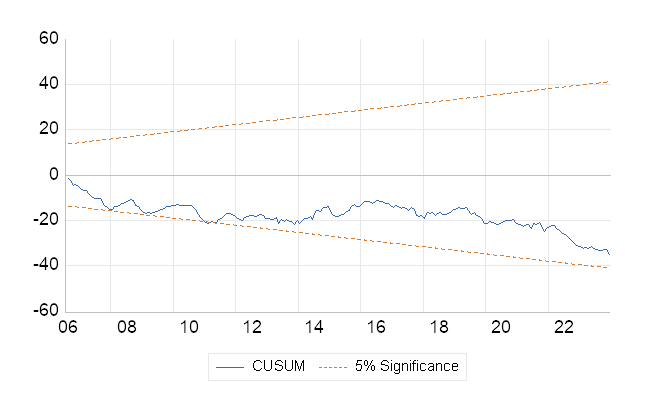
\includegraphics[scale=0.9]{annexes/cusum_nardl_logequity.png}
    \label{fig:msih_resids}
\end{figure}

\begin{figure}[H]
    \centering
    \caption{Test de normalité sur les résidus du modèle NARDL sur le LOGEQUITY.}
    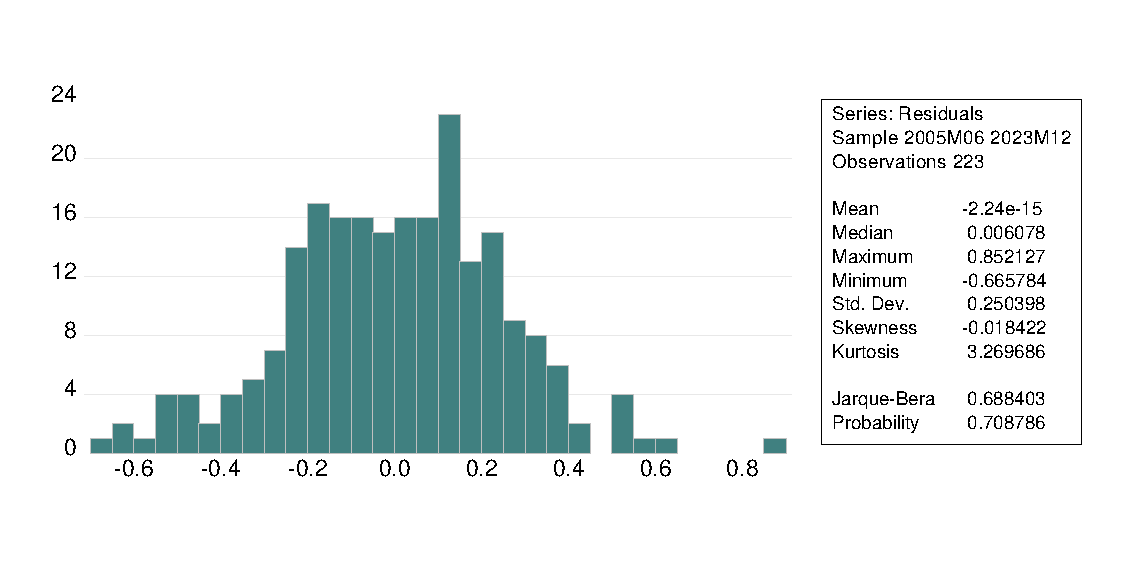
\includegraphics[scale=0.8]{annexes/normalite_nardl_logequity.pdf}
    \label{fig:normalite_nardl_logequity}
\end{figure}

\begin{figure}[H]
    \centering
    \caption{Test d'autorrélation sur les résidus du modèle NARDL sur le LOGEQUITY.}
    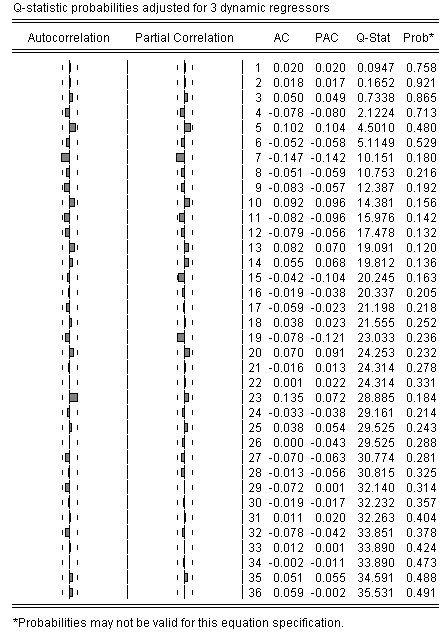
\includegraphics[scale=0.8]{annexes/autorrelation_nardl_logequity.png}
    \label{fig:correlo_nardl_equity}
\end{figure}

\begin{table}[H]
    \centering
    \sffamily
    \caption{Test ARCH sur les résidus du modèle NARDL sur le LOGEQUITY.}
    \label{tab:arch_nardl_logequity}
    \resizebox{0.8\textwidth}{!}{\begin{tabular}{lrrrr}
\multicolumn{2}{l}{Heteroskedasticity Test: ARCH}&\multicolumn{1}{c}{}&\multicolumn{1}{c}{}&\multicolumn{1}{c}{}\\
[4.5pt] \hline \\ [-4.5pt]
\multicolumn{1}{l}{F-statistic}&\multicolumn{1}{r}{$1.520254$}&\multicolumn{2}{l}{Prob. F(10,202)}&\multicolumn{1}{r}{$0.1341$}\\
\multicolumn{1}{l}{Obs*R-squared}&\multicolumn{1}{r}{$14.90839$}&\multicolumn{2}{l}{Prob. Chi-Square(10)}&\multicolumn{1}{r}{$0.1354$}\\
[4.5pt] \hline \\ [-4.5pt]
\multicolumn{1}{c}{}&\multicolumn{1}{c}{}&\multicolumn{1}{c}{}&\multicolumn{1}{c}{}&\multicolumn{1}{c}{}\\
\multicolumn{1}{l}{Test Equation:}&\multicolumn{1}{c}{}&\multicolumn{1}{c}{}&\multicolumn{1}{c}{}&\multicolumn{1}{c}{}\\
\multicolumn{2}{l}{Dependent Variable: RESID\textasciicircum 2}&\multicolumn{1}{c}{}&\multicolumn{1}{c}{}&\multicolumn{1}{c}{}\\
\multicolumn{2}{l}{Method: Least Squares}&\multicolumn{1}{c}{}&\multicolumn{1}{c}{}&\multicolumn{1}{c}{}\\
\multicolumn{3}{l}{Sample (adjusted): 2006M04 2023M12}&\multicolumn{1}{c}{}&\multicolumn{1}{c}{}\\
\multicolumn{4}{l}{Included observations: 213 after adjustments}&\multicolumn{1}{c}{}\\
\multicolumn{6}{l}{HAC standard errors \& covariance}\\
\multicolumn{2}{l}{bandwidth = 5.0000)}&\multicolumn{1}{c}{}&\multicolumn{1}{c}{}&\multicolumn{1}{c}{}\\
[4.5pt] \hline \\ [-4.5pt]
\multicolumn{1}{c}{Variable}&\multicolumn{1}{r}{Coefficient}&\multicolumn{1}{r}{Std. Error}&\multicolumn{1}{r}{t-Statistic}&\multicolumn{1}{r}{Prob.}\\
[4.5pt] \hline \\ [-4.5pt]
\multicolumn{1}{c}{C}&\multicolumn{1}{r}{$0.042386$}&\multicolumn{1}{r}{$0.010532$}&\multicolumn{1}{r}{$4.024389$}&\multicolumn{1}{r}{$0.0001$}\\
\multicolumn{1}{c}{RESID\textasciicircum 2(-1)}&\multicolumn{1}{r}{$0.111010$}&\multicolumn{1}{r}{$0.057992$}&\multicolumn{1}{r}{$1.914230$}&\multicolumn{1}{r}{$0.0570$}\\
\multicolumn{1}{c}{RESID\textasciicircum 2(-2)}&\multicolumn{1}{r}{$-0.035793$}&\multicolumn{1}{r}{$0.047757$}&\multicolumn{1}{r}{$-0.749473$}&\multicolumn{1}{r}{$0.4544$}\\
\multicolumn{1}{c}{RESID\textasciicircum 2(-3)}&\multicolumn{1}{r}{$-0.058386$}&\multicolumn{1}{r}{$0.061871$}&\multicolumn{1}{r}{$-0.943674$}&\multicolumn{1}{r}{$0.3465$}\\
\multicolumn{1}{c}{RESID\textasciicircum 2(-4)}&\multicolumn{1}{r}{$0.131238$}&\multicolumn{1}{r}{$0.096583$}&\multicolumn{1}{r}{$1.358814$}&\multicolumn{1}{r}{$0.1757$}\\
\multicolumn{1}{c}{RESID\textasciicircum 2(-5)}&\multicolumn{1}{r}{$-0.027346$}&\multicolumn{1}{r}{$0.077849$}&\multicolumn{1}{r}{$-0.351272$}&\multicolumn{1}{r}{$0.7258$}\\
\multicolumn{1}{c}{RESID\textasciicircum 2(-6)}&\multicolumn{1}{r}{$0.143302$}&\multicolumn{1}{r}{$0.085976$}&\multicolumn{1}{r}{$1.666764$}&\multicolumn{1}{r}{$0.0971$}\\
\multicolumn{1}{c}{RESID\textasciicircum 2(-7)}&\multicolumn{1}{r}{$0.093158$}&\multicolumn{1}{r}{$0.051755$}&\multicolumn{1}{r}{$1.799959$}&\multicolumn{1}{r}{$0.0734$}\\
\multicolumn{1}{c}{RESID\textasciicircum 2(-8)}&\multicolumn{1}{r}{$0.038932$}&\multicolumn{1}{r}{$0.078221$}&\multicolumn{1}{r}{$0.497717$}&\multicolumn{1}{r}{$0.6192$}\\
\multicolumn{1}{c}{RESID\textasciicircum 2(-9)}&\multicolumn{1}{r}{$-0.065832$}&\multicolumn{1}{r}{$0.053711$}&\multicolumn{1}{r}{$-1.225672$}&\multicolumn{1}{r}{$0.2217$}\\
\multicolumn{1}{c}{RESID\textasciicircum 2(-10)}&\multicolumn{1}{r}{$-0.021592$}&\multicolumn{1}{r}{$0.054195$}&\multicolumn{1}{r}{$-0.398420$}&\multicolumn{1}{r}{$0.6907$}\\
[4.5pt] \hline \\ [-4.5pt]
\multicolumn{1}{l}{R-squared}&\multicolumn{1}{r}{$0.069992$}&\multicolumn{2}{l}{Mean dependent var}&\multicolumn{1}{r}{$0.061331$}\\
\multicolumn{1}{l}{Adjusted R-squared}&\multicolumn{1}{r}{$0.023952$}&\multicolumn{2}{l}{S.D. dependent var}&\multicolumn{1}{r}{$0.092965$}\\
\multicolumn{1}{l}{S.E. of regression}&\multicolumn{1}{r}{$0.091845$}&\multicolumn{2}{l}{Akaike info criterion}&\multicolumn{1}{r}{$-1.887173$}\\
\multicolumn{1}{l}{Sum squared resid}&\multicolumn{1}{r}{$1.703961$}&\multicolumn{2}{l}{Schwarz criterion}&\multicolumn{1}{r}{$-1.713586$}\\
\multicolumn{1}{l}{Log likelihood}&\multicolumn{1}{r}{$211.9840$}&\multicolumn{2}{l}{Hannan-Quinn criter.}&\multicolumn{1}{r}{$-1.817021$}\\
\multicolumn{1}{l}{F-statistic}&\multicolumn{1}{r}{$1.520254$}&\multicolumn{2}{l}{Durbin-Watson stat}&\multicolumn{1}{r}{$1.965907$}\\
\multicolumn{1}{l}{Prob(F-statistic)}&\multicolumn{1}{r}{$0.134090$}&\multicolumn{1}{c}{}&\multicolumn{1}{c}{}&\multicolumn{1}{c}{}\\
[4.5pt] \hline \\ [-4.5pt]
\end{tabular}

}
\end{table}

\addtocontents{toc}{\protect\setcounter{tocdepth}{3}}

\restoregeometry

% Listes des figures et tables
\newpage

\addcontentsline{toc}{section}{Liste des figures}
\listoffigures

\newpage

\addcontentsline{toc}{section}{Liste des tables}
\listoftables

\newpage

\addcontentsline{toc}{section}{Bibliographie}
\begin{thebibliography}{MMM99}

\bibitem[Adam et Hendry]{Aglietta}
Adam C., et Hendry S., 
\textit{Le modèle vectoriel à correction d'erreur basé sur M1 : quelques extensions et applications},
Banque du Canada Working Paper, 2010.

\bibitem[Aglietta et Valla]{Aglietta}
Aglietta M. et Valla N., 
\textit{Macroéconomie financière}, 6e édition,
La Découverte, 2017.

\bibitem[Allen et McAleer]{Allen et McAleer}
Allen D. et McAleer M., 
\textit{A Nonlinear Autoregressive Distributed Lag (NARDL) Analysis of West Texas Intermediate Oil Prices and the DOW JONES Index}, Erasmus University Digital Repository,
2020.

\bibitem[Allen et al.]{Allen}
Allen F., Covi G., Gu X., Kowalewski O., Montagna M.,
\textit{The Interbank Market Puzzle}, 
2019.

\bibitem[Ang et Timmermann]{Ang et Timmermann}
Ang A. et Timmermann A., 
\textit{Regime Changes and Financial Markets}, Annual Review of Financial Economics, vol. 4, no. 1, pp. 313-337, 2012.

\bibitem[Arrata et al.]{Arrata}
Arrata W., Nguyen B., Rhamoun-Rousseau I. et Vari M.,
\textit{Eurosystem's asset purchases and money market rates}, 
Banque de France Working paper, 2017.

\bibitem[Balcilar et Ozdemir]{Balcilar et Ozdemir}
Balcilar M. et Ozdemir Z. A., 
\textit{Asymmetric and Nonlinear Adjustment in House Prices: Evidence from Threshold Autoregressive and Markov-Switching Models}, 
Economic Modelling, vol. 35, pp. 536-544, 2013.

\bibitem[Bech et Monnet]{Bech et Monnet}
Bech M., Monnet C., 
\textit{A search-based model of the interbank money market and monetary policy implementation}, No 529, BRI Working Paper, 2015.

\bibitem[Bech et Hobijn]{Bech et Hobijn}
Bech M. et Hobijn B.,
\textit{Technology Diffusion within Central Banking: The Case of Real-Time Gross Settlement},
International Journal of Central Banking, 2007.

\bibitem[Bennani et al.]{Clerc}
Bennani T., Clerc L., Coudert V., Dujardin M., Idier J.,
\textit{Politiques macroprudentielles},
Pearson, 2017.

\bibitem[Bianchi et Civelli]{Bianchi et Civelli}
Bianchi F. et Civelli A, 
\textit{Globalization and Inflation: Structural Evidence from a Time Varying VAR Approach}, 
Working Paper 13-20, Duke University, Department of Economics, 2013.

\bibitem[Bianchi]{Bianchi}
Bianchi F., 
\textit{The Great Depression and the Great Recession: A View from Financial Markets}, 
NBER Working Papers 21056, National Bureau of Economic Research, Inc., 2015.

\bibitem[Binder et Gross]{Binder et Gross}
Binder M. et Gross M., 
\textit{Regime Switching Global Vector AutoRegressive Model}, 
ECB Working Paper, n°1569, 2013.

\bibitem[Bismans et Damette]{Bismans}
Bismans F. et Damette O., 
\textit{Économétrie dynamique : modèles et applications}, 
Ellipses, 2023.

\bibitem[Bourbonnais et Terraza]{Terraza}
Bourbonnais R., Terraza M.,
\textit{Analyse des séries temporelles}, 3e édition,
Dunod, 2010.

\bibitem[Brunnermeier et Pedersen]{Brunnermeier et Pedersen}
Brunnermeier M. K. et Pedersen L. H., 
\textit{Market Liquidity and Funding Liquidity},
The Review of Financial Studies, vol. 22, no. 6, pp. 2201-2238, 2009.

\bibitem[Colletaz]{Colletaz}
Colletaz G.,
\textit{Introduction à la cointégration}, 2020.

\bibitem[Dameron]{Dameron}
Dameron P.,
\textit{Mathématiques des modèles dynamiques : analyse dynamique}, 
Economica, 2001.

\bibitem[Duca et Peltonen]{Duca et Peltonen}
Duca M. L. et Peltonen T. A.,
\textit{Assessing Systemic Risks and Predicting Systemic Events}, Journal of Banking \& Finance, vol. 37, no. 7, pp. 2183-2195, 2013.

\bibitem[Engle et Granger]{Engle et Granger}
Engle R. F. et Granger C. W. J., \textit{Co-integration and error correction: representation estimation and testing}, 
Econometrica, vol.55, n°2, mars 1987.

\bibitem[Engle et Yoo]{Engle et Yoo}
Engle R. F. et Yoo B. S., \textit{Forecasting and testing in co-integrated systems}, 
Journal of Econometrics, p.143-159, 1987.

\bibitem[Francq et Zakoian]{Francq et Zakoian}
Francq C., et Zakoian J-M.,
\textit{Modèles GARCH : structure, inférence statistique et applications financières},
Economica, 2009.

\bibitem[Gourieroux et Monfort]{Gourieroux et Monfort}
Gourieroux C. et Monfort A., 
\textit{Séries temporelles et modèles dynamiques},
2e édition, Economica, 1999.

\bibitem[Hamilton]{Hamilton} 
Hamilton, J. D.,
\textit{A New Approach to the Economic Analysis of Nonstationary Time Series and the Business Cycle}, Econometrica, vol. 57, no. 2, pp. 357-384, 1989.

\bibitem[Holló et al.]{Hollo} 
Holló D., Kremer M., et Lo Duca M., 
\textit{CISS - A Composite Indicator of Systemic Stress in the Financial System},
European Central Bank Working Paper Series, no. 1426, Mars, 2012.

\bibitem[Hubrich et Tetlow]{Hubrich et Tetlow}
Hubrich K. et Tetlow R., 
\textit{Financial Stress and Economic Dynamics : the Transmission of Crises},
ECB Working Paper, N°1728, 2O14.

\bibitem[Hurlin]{Hurlin}
Hurlin C., 
\textit{Modèle à retards distribués et modèles ARDL},
Université d'Orléans, Avril, 2O19.

\bibitem[Kole et Van Dijk]{Kole et Van Dijk}
Kole E. et Van Dijk D., 
\textit{Moments, Shocks and Spillovers in
Markov-Switching VAR Models},
Tinbergen Institute Discussion Paper, 2023.

\bibitem[Greene]{Greene}
Greene W.,
\textit{Économétrie},
5e édition,
Pearson, 2005.

\bibitem[Johansen et Juselius]{Johansen}
Johansen S. et Juselius K.,
\textit{ Maximum likelihood estimation and
inference on cointegration – with applications to the demand for money},
Oxford Bulletin of Economics and Statistics,
1990.

\bibitem[Kibala Kuma]{Kibala}
Kibala Kuma J., 
\textit{Modélisation ARDL, Test de cointégration aux bornes et Approche de Toda-Yamamoto: éléments de théorie et pratiques sur logiciels},
Licence, Congo-Kinshasa, 2018.

\bibitem[Kibala Kuma]{Kibala}
Kibala Kuma J., 
\textit{Cointégration et modèle à correction d'erreur : pratique sur Eviews},
Licence, Congo-Kinshasa, 2018.

\bibitem[Kibala Kuma]{Kibala}
Kibala Kuma J., 
\textit{Le modèle VAR structurel : élements de théorie et pratiques sur logiciel},
Licence, Congo-Kinshasa, 2018.

\bibitem[Krolzig]{Krolzig}
Krolzig H. M., 
\textit{Markov-Switching Vector Autoregressions: Modelling, Statistical Inference, and Application to Business Cycle Analysis},
Berlin: Springer-Verlag, 1997.

\bibitem[Ruch et Chabanol]{Ruch et Chabanol}
Ruch J.J. et Chabanol M.L., 
\textit{Chaînes de Markov},
Préparation à l'agrégation Bordeaux 1, 2013.

\bibitem[Mignon]{Mignon}
Mignon V.,
\textit{Économétrie : théorie et applications},
2e édition,
Economica, 2022.

\bibitem[Mills]{Mills}
Mills T.C.,
\textit{The Econometric Modelling of Financial Time Series},
2nd edition, Cambridge University Press.

\bibitem[Narayan]{Narayan}
Narayan P.K.,
\textit{Reformulating Critical Values for the Bounds F-Statistics
Approach to Cointegration : An Application to the Tourism Demand Model for Fiji}, 
Department of Economics, Discussion Papers, No.02/04, Monash University, 2004.

\bibitem[Perez et al.]{Perez}
Pérez S., Yasmina, Lozoya C., García Ramos L. et Arregui Gil J-M.,
\textit{Spread between the euro short-term rate (€STR) and the deposit facility rate}, Economic Bulletin - Banco de España, 2023.

\bibitem[Pesaran et Shin]{Pesaran et Shin}
Pesaran M.H., et Shin Y.,
\textit{An Autoregressive Distributed-Lag Modelling
Approach to Cointegration Analysis},
Econometrics and Economic Theory, p. 371-413, 1998.

\bibitem[Pesaran et al.]{Pesaran}
Pesaran M.H., Shin Y., Smith R.,
\textit{Bounds testing approaches to the analysis of level relationships},
Journal Applied of Econometrics, 2001.

\bibitem[Phillips Perron]{Phillips Perron}
Phillips, P. et Perron, P.,
\textit{ Time Series Regression with a Unit Root},
Econometrica, vol.55, No.2, Mars, pp. 277-301, 1987.

\bibitem[Phillips Perron]{Phillips Perron}
Phillips, P. et Perron, P.,
\textit{Testing for a Unit Root in Time Series Regression},
Biometrica, Vol.75, pp. 335-46, 1988.

\bibitem[Pinshi]{Pinshi}
Pinshi C., 
\textit{Repenser le modèle à correction d’erreurs dans l’analyse macroéconométrique}, 
Une revue. 2021

\bibitem[Schrimpf et Sushko]{Schrimpf et Sushko}
Schrimpf A., Sushko V.,
\textit{Après le LIBOR : une introduction aux nouveaux taux
de référence}, Rapport trimestriel BRI, 2019.

\bibitem[Schorderet]{Schorderet}
Schorderet Y., 
\textit{Asymmetric Cointegration},
University of Geneva, 2003

\bibitem[Shin et al.]{Shin}
Shin Y., Yu B., et Greenwood-Nimmo M.,
\textit{Modelling asymmetric cointegration and dynamic multipliers in a nonlinear ARDL framework}, 
The Festschrift in Honor of Peter Schmidt.: Econometric Methods and Applications, p. 281–314, 2014.

\bibitem[Vari]{Vari}
Vari M., 
\textit{Monetary policy transmission with interbank market fragmentation}, 
2016.

\newblock

\bibitem[BCE]{BCE}
Banque Centrale Européenne : \texttt{www.ecb.europa.eu}

\bibitem[BDF]{BDF}
Banque de France : \texttt{www.banque-france.fr}

\end{thebibliography}


% Table des matières complète à la fin
\clearpage
\etocsetnexttocdepth{3} % Inclut les sous-sections
\etocarticlestyle
\addcontentsline{toc}{section}{Table des matières}
\tableofcontents

\newpage
    % Page avec l'arrière-plan
    \AddToShipoutPictureBG*{\BackgroundPicBackPage}
    \thispagestyle{empty}
    % Ajoutez votre contenu ici si nécessaire
    \null % Placeholder si aucun contenu n'est nécessaire
\end{document}

